\chapter{GPU architecture}
\label{chap:gpu-architectures}


%\section{GPU vs. CPU}
\label{sec:gpu-vs.-cpu}

% \section{GPU as a general-purpose computing processor}
% \label{sec:gpu-as-computational}

GPUs are conventionally utilized for video accelerator. The programs running on
GPU are often written using some special programming languages
(Sect.\ref{sec:programming-with-gpu}), and such programs are called shaders
(Sect.\ref{sec:shader}).


The nature of image/video processing requires handling a large amount of data of
the same type (pixel, voxel). Also, precision is not important for theses types
of data for displaying purpose. Because of that, we will learn the main
differences between the two architectures between CPU and GPU in this section.


\section{Cores}
\label{sec:cores}

\textcolor{red}{The concept of ``cores'' are two different things between  CPU
vs. GPU}. 


\subsection{CPU core}

A CPU core, e.g. Intel Core-2, has a vector unit, that can do multiply/add
several operands at once. Intel Itanium Tukwila CPU core,
Fig.\ref{fig:Intel_Itanium_Tukwila_core}, has
\begin{enumerate}
  \item 6-wide instruction fetch, issue and execution: 6 integer units, 2 FP
  units, 4 memory units, 3 branch units
  \item 1 cycle L1 data cache
  \item separate  L1I, L1D, L2I, and L2D caches (I=instruction, D=data)
  \item short 8 state pipeline
  \item 4k/8k/16k page size support in first level data TLB
\end{enumerate}

A more equivalent comparison would be between CPU core and GPU streaming
multiprocessor (SM) which is a group of SPs - to be discussed later -
Sect.\ref{sec:stre-mult-sm}). A CPU core uses a lot more resources/gates on
control structures, leaving a much higher ratio of control-gate to
calculation-gate in CPU than found in GPU.

\subsection{GPU core}

GPU cores are simpler and are more speciallized than CPU cores
In general, a GPU core is a scaled down version of a CPU core and is more likely
an ALU (arithmetic logic unit) - a functional unit in CPU core,
Fig.\ref{fig:gpu.cpu_core}. 

GPU cores are put into different types, depending on their specialized
functions, e.g. some are designed to handle shading (or coloring) pixels, some
to handle shading vertex, etc. Thus, there are different names to call a GPU
core
\begin{itemize}
  \item a shader (in computer graphics field) 
  
  \item a streaming processor (SP) (GPUs with universal shader architecture)
  
  \item CUDA core (Nvidia CUDA architecture) - special name given to SP in Nvidia's GPUs.
\end{itemize}

\begin{figure}[hbt]
  \centerline{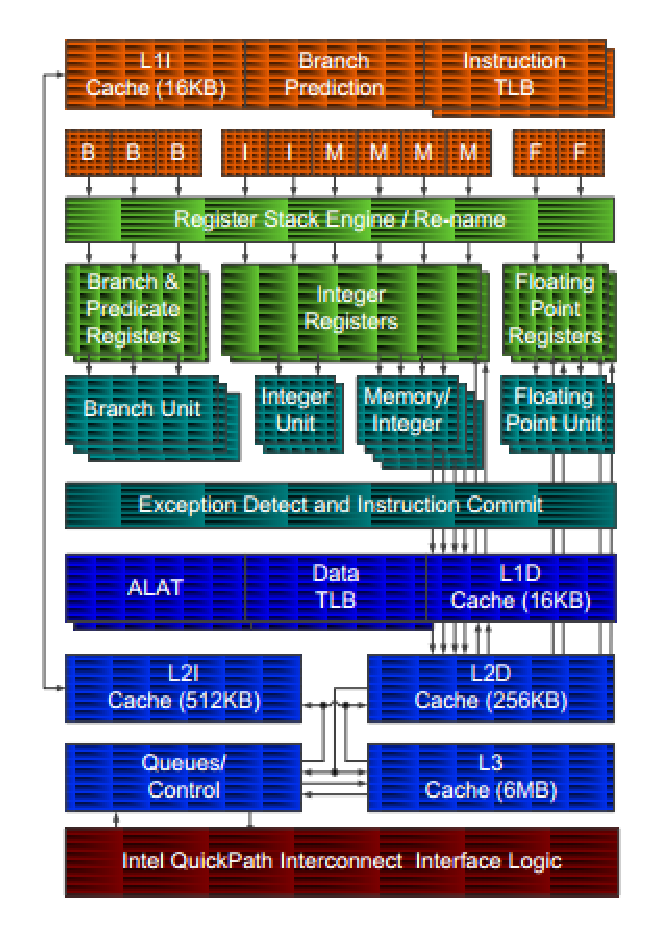
\includegraphics[height=5cm,
    angle=0]{./images/Intel_Itanium_Tukwila_core.eps}}
  \caption{Intel Itanium Tukwila CPU core}
  \label{fig:Intel_Itanium_Tukwila_core}
\end{figure}

With many more number of cores in GPU than in CPU, the GPU cores are much
simpler and smaller. A major fraction of GPU is occupied by the transistors
(higher density than that in CPU), i.e. CPU run a lot hotter than the average
CPU, especially when playing games.

  
Both Nvidia and ATI's AMD manufacture GPUs with a slightly difference in
hardware design
\begin{itemize}
  \item Nvidia GPU: fewer cores but the cores are capable of more complex tasks
  than AMD cores
  
  \item AMD GPU: more cores that can significantly speedup the calculations
  (but less flexible)
\end{itemize}


In terms of speed (Sect.\ref{sec:clock-cycles-speeds}),  ATI's SP is different
from Nvidia's SP (CUDA core): ATI's SP run at core speed, while Nvidia's SP  run
well beyond core speed. ATI's SP can't do texture and shading at the same time;
while Nvidia's SP can. In recent CUDA architecture, all Nvidia CUDA core are
identical (unified); while some of ATI's core are missing some capabilities,
e.g. one out of every 4 ATI's core is missing the dot-product hardwares. To make
it easier, we will focus on the comparison between Intel CPU core and Nvidia GPU
cores (if not mention explicitly).
  
\begin{framed}
  When comparing CPU core vs. GPU core, we look into 
  \begin{enumerate}
    \item CPU complete: more complicated, with cache, registers. In GPU,
    cache only available at streaming multiprocessor (SM) level from 2nd
    generation. Also, registers are not part of GPU core.
    \item instruction set: CPU core can handle complicated operations, but CPU
    core only does simple arrhithmetic operation, and a separate special
    functional unit is required to do complicated operations like square-root,
    exponential function.
  \end{enumerate}
\end{framed}
  
Cores\footnote{\url{http://en.wikipedia.org/wiki/Multi-core_processor}}:
 
  \begin{itemize}
  \item CPU: Intel Nehalem (2,4,6,8,10, 12), AMD Opteron
    (1,2,4,6,8,12), UltraSPARC T2 ({\it codename: Niagra 2}) (8 CPU cores),
    UltraSPARC T3 (16 CPU cores).
    
    NOTE: Intel's Tera-scale Research Program introduced many-core CPU Polaris
    (80-core processor in 2007) with cores here are simpler than CPU cores used
    in multi-core CPUs. Each core has 2 floating-point engines.
    
    IntellaSys introduced SEAforth 40C18 (40-core processor) embeded processor
    in 2008. Each core is a complete computer with
    its own RAM and ROM (64-word each) and can operate asynchronously with other
    cores
    \footnote{\url{http://dbaspot.com/arch/419828-intellasys-seaforth-40c18-40-core-processor-guy-macon.html}}.
    To program on it, we use  VentureForth, a Forth-based IDE in both Windows and Linux.
    
\begin{framed}
  Until May, 2010, the fastest CPU chip of Intel,
  {\it codename ``Knights Ferry''}, has 32 CPU cores and is being used
  for development purpose. The first commercial product will
  include more than 50 cores and to be called ``Knights Corner''
  (Sect.\ref{sec:Intel_GPGPU}).
\end{framed}
    
  \item GPU G80 (e.g. GeForce 8800 GTX) - Nov, 2006: the first generation of
  Tesla architecture GPU, with 128 CUDA cores (shaders), use 90nm technology
  (Sect.\ref{sec:g80g92-architecture}). G80 has 690M transistors.
  
   
  \item[*] Tesla 1st gen (chip G80, no VGA/DVI output) - C870
  
  \item GPU G92 (e.g. GeForce 8800 GT): use 65nm technology, with 754M
  transistors.
  
  \item GPU GT200 (e.g. GeForce GTX 280): the second generation of Tesla
  architecture that uses 65nm (GT200A) and 55nm (GT200B), with 240 cores and
  1.4B transistors.
  
  NOTE: GT = Graphics Tesla, GF = Graphics Fermi, GK =  Graphics Kepler
  
  \item [*]Tesla 2nd gen (chip GT200a/b, no VGA/DVI output) -
    C1060/S1070
    \item [NOTE] Project G200b/GTX285 use 55nm technology
    \item [NOTE] Project G212/G214 failed to use 45nm technology
    
  \item GPU GF100 - theory 512 cores, yet due to 40nm architecture
    restrictions, some of them are disabled (e.g. GeForce GTX 480 has
    480 cores, GeForce GTX 470 has 448 cores). 
    
  \item [*] Tesla 3rd gen (codename: {\it Fermi}): C2050/C2070 with 512 cores
  grouped into 16 SMs.
  \item [*] chip GTX 470, with DVI output - use GF100; GTX 475 use GF104.
  \item 
    \textcolor{blue}{GPU GF104/GF106/GF108: a remake of
      GF100 by making a smaller verion of Fermi architecture rather than taking
      larger GPU. So, they have less cores, less
      memory, lower bandwidth} (Jul, 2010). 
      
      \item [*] GTX 460, GTS 455 use GF104 with 336 cores, 675MHz graphics clock
      (i.e. 1350 processor clock) and 1GB 1.8GHz memory. GTS 455 is, however,
      slower than GTX 460.
%      \item [*] GTX

   \item GPU GK110 - uses 28nm technology features 1024 CUDA cores, with 7.1 billion transistors.
   
    
   \item [*] Tesla 4th gen (codename: {\it Kepler}): use GK110 
   
   \item \textcolor{blue}{GPU GK100/GK102/: lower level of GK110 targetting to
   computer graphics}. GeForce GTX 680 has 10.0'' long; GeForce GTX 690 has
   11.0'' long while GeForce GTX Titan is 10.5'' long (AMD Radeon HD 7970 is
   11.5'' long).
   
   \item Tesla Maxwell GM200 uses 28-nm FFN with 8 billion transistors.
   
   \item Tesla P100 GPU - uses 16nm FinFET, with 15.3 billion transistor GPU
   
   \item  GV100 GPU - use new TSMC 12 nm FFN (FinFET NVIDIA) with 21.1 billion transistors with a die size of 815 mm$^2$.
  
  
  \end{itemize}


\begin{figure}[hbt]
  \centerline{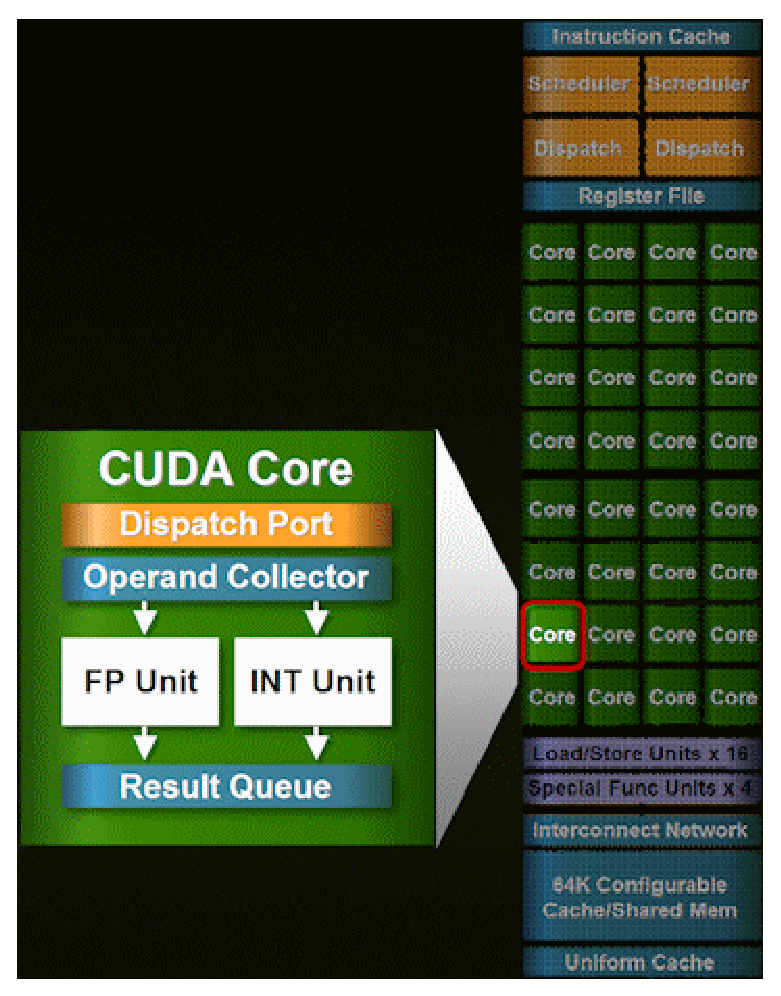
\includegraphics[height=7cm,
    angle=0]{./images/gpu_core.eps},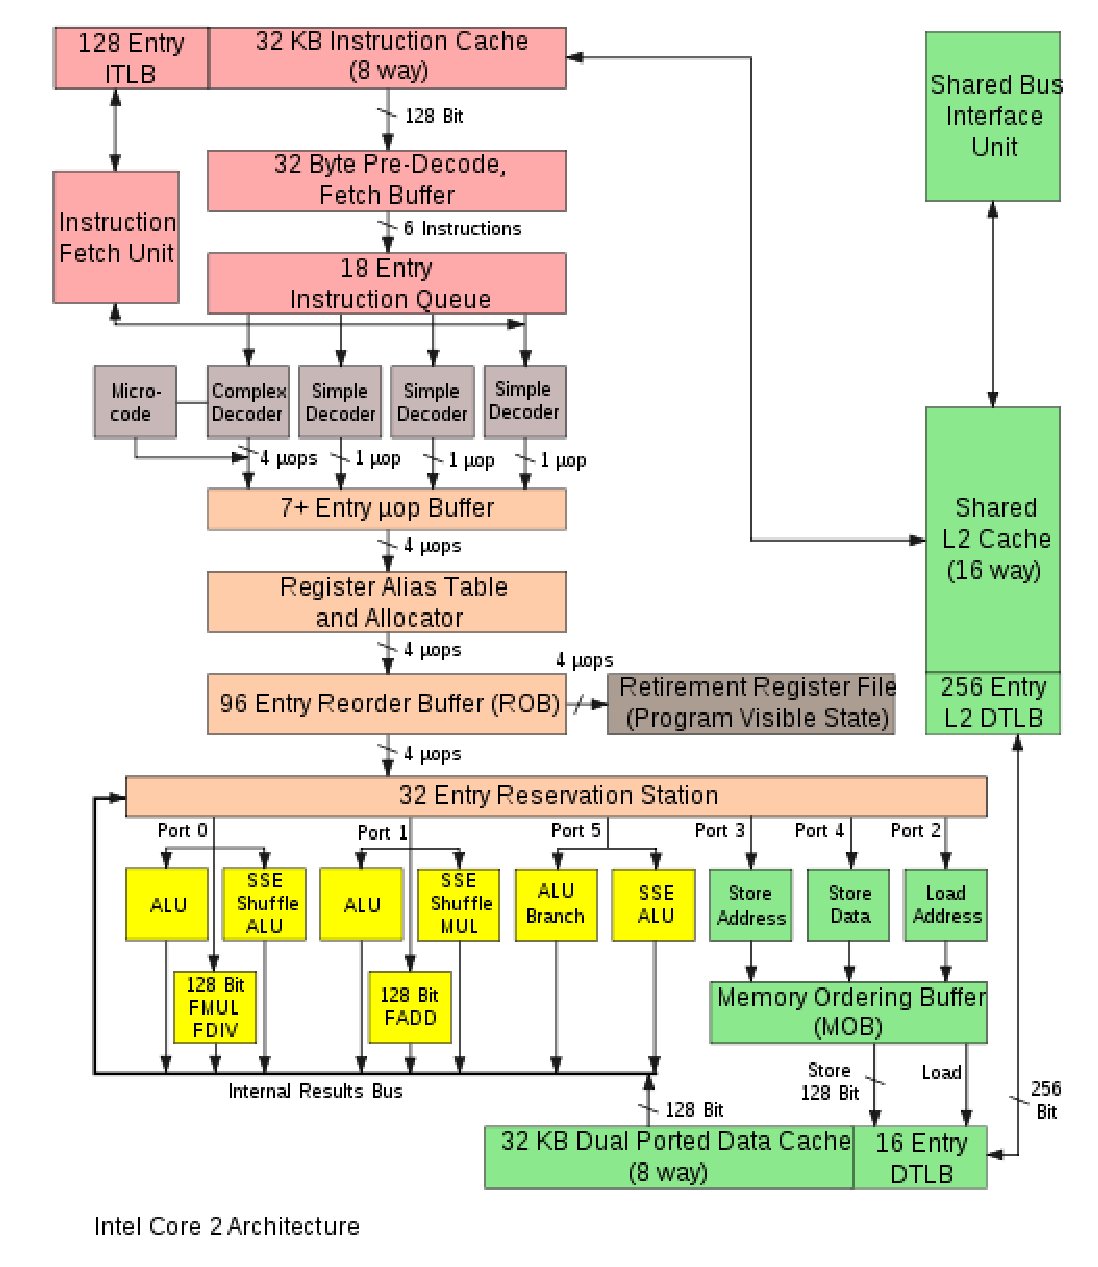
\includegraphics[height=7cm,
    angle=0]{./images/core2_intel.eps}}
 \caption{(A) GTX280 GPU core, (B) Intel Core2
 \footnote{\url{http://blog.langly.org/2009/11/17/gpu-vs-cpu-cores/}}}
\label{fig:gpu.cpu_core}
\end{figure}

A CPU core can execute four 32-bit instruction per clock (using 128-bit SSE) or
eight 32-bit instructions (using AVX 256-bit registers). A GPU like Radeon HD
5970 can execute 32000 32-bit instructions per clock (using 32000 ALUs or
shaders). Even a typical multi-core CPU has more core (upto 6, 8 or 12) and
higher frequency clock (2000-3000 MHz vs. 735MHz in Radeon HD 5970), a Radeon
GPU still runs more than 5x faster, yet with a cheaper cost (350\$ vs. a
12-core CPU 4700\$). Recently, Intel have introduced a GPU-like platform called
Xeon Phi, with 86 cores that can deliver 1 TFLOPS double-precision.

References:
\begin{itemize}
\item \url{http://blog.langly.org/2009/11/17/gpu-vs-cpu-cores/}
\end{itemize}



\section{Memory hierarchy in GPU}

\subsection{Register files}
\label{sec:register-files}

A {\bf register} (or register file) refers to the kind of storage with smallest
access latency (extremely fast memory space, with access time is almost zero).
Accessing data in registers just take a few bits of encoding - unlike memory
address, where we need a longer address to refer to a variable.
Small access latency means an expensive in hardware implementation; thus the
number of available registers in CPUs are very small (read Chapter {\it X86 and
X86-64} in Fortran book).


GPGPU has been designed with a large number of register files. The goal is
minimize the latency in thread switching, i.e. lightweight thread. This is not
the case in CPU, i.e. heavy-weight thread, as each thread switching requires
backing up the data in the register files (Sect.\ref{sec:threads-1}).

Early GPU has register file of 32-bit. Recent GPUs has register file of
64-bit (Fermi GPU).  CPU registers are more complex with 128-bit, and
recently 256-bit.
% 
% However, the memory space is limited. The memory is splitted into a number
% of 32-bit or 64-bit register file, depending on architectures. 
  \begin{itemize}
  \item CPUs: dozens of registers, e.g. SPARCS v8 has 160
    general-purpose registers (yet only 32 are available to software =
    8 global registers + 24 forms register window, each window has 8
    local
    registers\footnote{local registers are used for retaining local
      values across function calls}
    and shares 8 registers with adjacent
    windows\footnote{the shared registers are used for passing
      function parameters and returning values}),
    16 64-bit
    registers\footnote{can be used as 32 single-precision registers or
      8 quad-precision registers}.
      
  \item Nvidia C870: 8192 32-bit registers
\item Nvidia Tesla C1060: 16384 32-bit registers
\item Nvidia Fermi C2050: 32768 32-bit registers
%\item AMD Cypress has 16384 128-bit registers
  \end{itemize}

% The maximum number of registers per SM (streaming multiprocessor) is
% \begin{itemize}
% \item 8192 in Tesla 1st gen (CC.1.0, CC.1.1)
% \item 16384 in Tesla 2nd gen (CC.1.2,CC.1.3)
% \item 32768 in Tesla 3rd gen (CC.2.0)
% \end{itemize}

For more information, read Sect.\ref{sec:register-memory} and
Sect.\ref{sec:registers-ptx}.


\subsection{Constant, Shared and Cache memory}
\label{sec:const-shar-cache}

Constant, shared and cache memory are fast access memory, yet slower than
Register file memory (Sect.\ref{sec:register-files}). Shared and cache are
on-chip memory, while constant memory reside on global device memory
(Sect.\ref{sec:constant-memory}, yet the mechanism for reading data from
constant memory allows the data to be cached in a cache-memory making it can be
accessed faster from the second read access.
% Amount of Constant, Shared and Cache Memory
  \begin{framed}
    A cache is a smaller, faster memory which stores copies of the
    data from the main memory location (RAM). Two main caches are
    {\bf instruction cache} (speed up instruction fetch) and
    {\bf data cache} (speed up data fetch and store). 
    \begin{itemize}
    \item CPU often have
      large cache to reduce the latency in data fetching, thus maximize
      performance of the sequential-execution model. 

    \item GPU, however, is designed to do multiple computation at the same
      time. Thus the hardware for execution units (arithmetic execution)
      take a large portion of the chip. As a result, GPU has a restricted
      amount of shared and cache memory. 
    \end{itemize}
    As off-chip memory access is high-latency, it's recommended to
    maximize using on-chip memory (constant, shared memory, cache) by
    having algorithms of high locality of memory access (to be
    discussed later).
  \end{framed}

Cache can be classified into L1, L2, and L3 cache. The lower the number the
faster memory access. In a multicore CPU architecture, L1 cache is accessible
for a single core, L3 is shared by all cores, and L2 is intermediate between L1
and L3 yet accessible by a single core (NOTE: access time $L1<L2<L3<$RAM).

\begin{mdframed}

Old CPUs has L1 cache and SRAM as L2 cache. In newer CPUs, L2 is moved into CPU,
i.e. both L1 and L2 on CPU, and they added L3 cache. Multicore CPU has L3 moved
to CPU as well, yet is shared by multicore in a single CPU, while L1 and L2 are
dedicated to a single core (except Intel Core 2 has 1MB-6MB L2 cache shared by 2
CPU cores and use this to communicate between 2 cores). Size: L1 cache (16-64KB
per core, for each instruction cache and data cache), L2 cache (256KB-1MB per
core, hold both  instruction and data).

Latency in x86 CPUs: L1 cache (2-3 clock cycles), L2 cache (10-12 clock cycles),
L3 cache (dozens of clock
cycles)\footnote{\url{http://www.tomshardware.com/forum/297190-28-about-cache}}.
\end{mdframed}

\subsection{Texture memory}

Unlike CPU where LD/ST units are an integral part of the CPU core, texturing and
render output are decoupled from the CUDA core, Fig.\ref{fig:GT200_texture}.
Here, the SM controller can read data either from the texture data (which can
be from L1 texture cache, L2 texture cache or global memory), general data
from the global memory; then process and save it to the global memory (in the
case of a graphics application, the result is passed to Raster Engine (ROP)).
So, what is texture memory? As shown in Fig.\ref{fig:GT200_texture}, there are
two specialized texture caches.

Memory in CPU RAM, CPU caches have locality in a single dimension because memory
addressing for most architectures is linear. Typically, data is fetched in
groups, defined by the {\bf cache line}. An example from Intel Itanium Tukwila
is given in Fig.\ref{fig:Intel_Itanium_Tukwila_cacheline}. Here, L1 cache is
4-way, L2 cache is 8-way and L3 cache is 12-way.
% If the data cache and
% instruction cache are separated.

\begin{figure}[hbt]
  \centerline{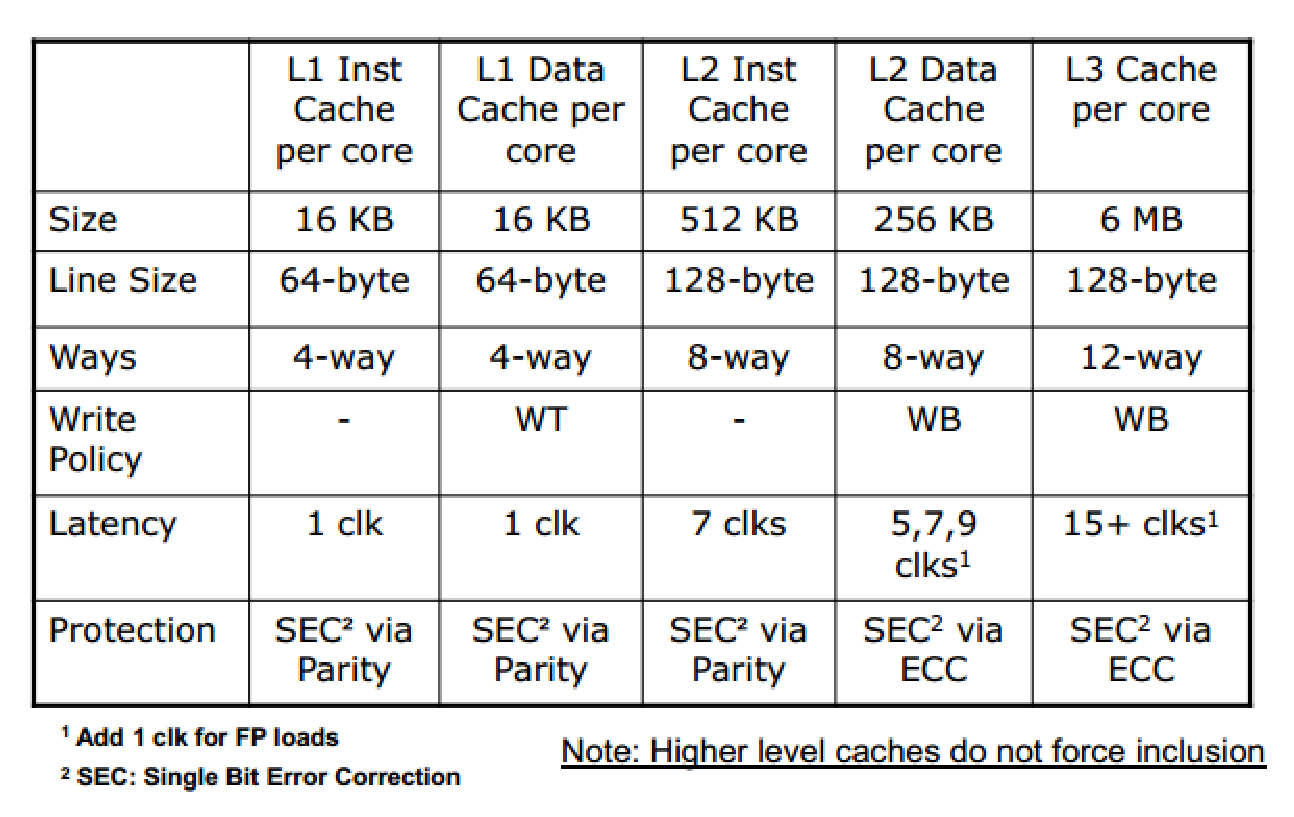
\includegraphics[height=5cm,
    angle=0]{./images/Intel_Itanium_Tukwila_cacheline.eps}}
  \caption{Cache line in Intel Itanium Tukwila CPU}
  \label{fig:Intel_Itanium_Tukwila_cacheline}
\end{figure}

\begin{mdframed}

Caches come in different forms and capacities. But now matter how large or small
they are, caches fall into one of the three categories: {\it direct mapped},
{\it n-way set associative}, and {\it fully associative},
Fig.\ref{fig:Cache_structures}. Depending which one is being used, a cache block
is identified using upto three information: tag, index, and offset. If a cache
slot is small enough to put one cache block, then it's direct mapped, and make
it easier to find the block, but it's not flexible about where to put the
blocks. In {\it n-way associative}, we have, example 2-way or 4-way associative
cache. In 2-way set, we can put two cache blocks in a slot or in 8-way set, we
can put a cache block in one of 8 different locations, i.e. giving some
flexibility.

The index is used to find the slot index, and the tag is used to find the block
within the set of cache blocks inside the slot. \textcolor{red}{The hardware is
very complicated with fully associative caches (as it requires parallel searchs
of all slots)}
\footnote{\url{http://csillustrated.berkeley.edu/PDFs/handouts/cache-3-associativity-handout.pdf}}
\end{mdframed}

\begin{figure}[hbt]
  \centerline{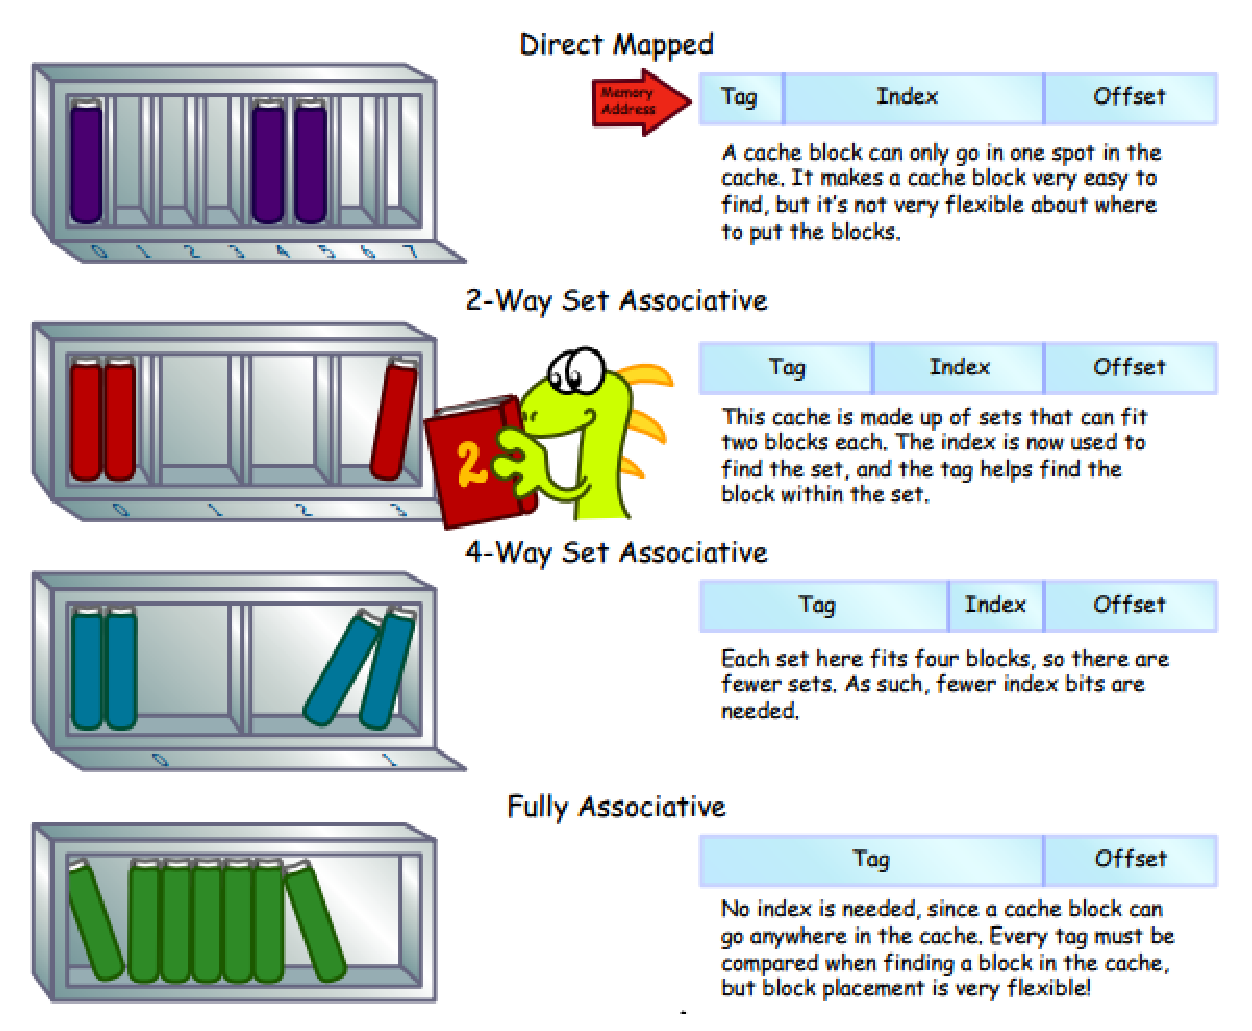
\includegraphics[height=5cm,
    angle=0]{./images/Cache_structures.eps}}
  \caption{A cache is like a bookshelf: how we divide the slot to put one or
  more books in each slot}
  \label{fig:Cache_structures}
\end{figure}


Suppose the cache line is 64-Byte, a
read of one data word (4Byte or 8Byte) results 64-Byte to be read. Most of the
time, the unused 56B-60B of data are in closed proximity to the original
requested data. GPU global memory are physically organized in a similar linear
layout (i.e. 2D or 3D data structures are ultimately mapped to 1D).

However, GPU has a special memory space that is designed to work with 2D data
(and recently with 3D data) that random access to any item in the array A[i,j]
take the same amount of time - known as {\bf texture memory}.
\textcolor{blue}{Texture memory in C1060 is specifically designed for optimal 2D
pixel/voxel-based memory access in graphical applications. Texture memory in
Fermi GF100 support both 2D and 3D pixel/voxel-based memory access}. NOTE:

\begin{enumerate}
  \item  texture caches are read-only and have no coherency. When a texture is written,
the entire texture cache hierarchy must be invalidated, rather than tracking the
validity of individual data within the address space. 
  \item unlike CPU cache that lowering latency (from 100ns to 7ns), GPU texture
  cache is used to avoid bandwidth and power consumption. 
\end{enumerate}

\begin{figure}[hbt]
  \centerline{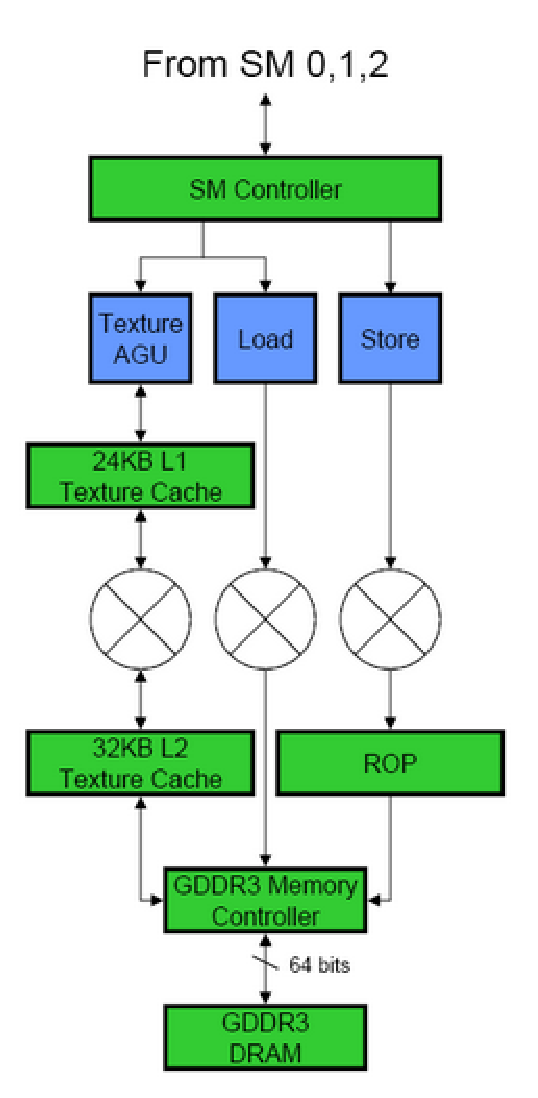
\includegraphics[height=5cm,
    angle=0]{./images/GT200_texture.eps}}
  \caption{Texture Unit, ROP and Memory Pipeline}
  \label{fig:GT200_texture}
\end{figure}


As texture-cache are designed for graphical applications, and access this memory
require using Texture CUDA Graphical APIs, it's not popularly used by a
general scientific high performance computing application.

  \begin{itemize}
  \item CPU: use large caches to convert long latency memory access to
    short cache sequential accesses,
    Fig.\ref{fig:Intel_Itanium_Tukwila_cacheline}. It thus uses sophisticated
    control to improve sequential execution.
    \begin{itemize}
    \item Intel Nehalem (32KB L1 instruction + 32KB L1 data (L1D)
      cache memory per core; 256KB L2 cache memory, 4-8MB L3 cache
      memory),
    \item AMD Opteron (64KB L1 instruction + 64KB L1D cache each core;
      1024KB L2 cache (single core), 2*1024 (dual-core), 512KB per
      core (quad-core); 1024KB L3 (quad-core Barcelona), 6MB L3 each
      core (quad-core Istanbul + Shanghai), 2*6MB L3 shared (8-12
      core))\footnote{\url{http://en.wikipedia.org/wiki/Opteron}}.
    \item Niagra 2 has 8KB L1D cache per CPU core. Totally, the chip
      has 4MB L2 cache with 8 banks.
    \end{itemize}
  \end{itemize}
  GPU uses small caches; which can be accesses in parallel. So, it
  boosts memory throughput via many, long latency but heavily
  pipelined caches.

  \begin{itemize}
  \item Tesla 1st gen C870 (per cluster = TPC = 2 SMs; 1 SM = 8 SPs):
    8KB read-only {\it constant-cache memory} (or just constant
    memory), 16KB L1 read-only texture cache (texture cache are
    originally designed for graphical applications). Totally, with 8
    clusters, a GPU has $8\times 8=64$KB constant-cache memory, and
    $16\times 8=128$KB L1 texture cache.

    The whole-chip L2 texture cache is also 128KB and is divided into
    6 banks.

    Per SM, it has 16KB shared memory (i.e. $8\times 2\times 16=256$KB
    shared-memory totally).

  \item Tesla 2nd gen C1060 (per cluster = TPC = 3 SMs; 1 SM = 8 SPs):
    6.4KB read-only constant memory; 24KB L1 read-only texture
    cache (partitioned into 3x8KB). Totally, with 10 clusters, a GPU has
    $6.4\times 10=64$KB constant memory and 10 x 24KB = 240KB L1 texture cache.

    The 256KB L2 texture cache is shared by all TPC and is divided
    into 8 banks, i.e. each bank is 32KB.

    Per SM, it has 24KB shared memory (i.e. $10\times 3\times
    24=720$KB). 

    \begin{framed}
      Only Fermi has true L1/L2 cache.  C870 and C1060 indeed have
      L1/L2 {\bf texture cache} which are originally designed to work
      with pixel/voxel-liked data. Texture caches were mostly useless
      when GPU run in compute mode (high-performance scientific
      applications); however, it's possible to use it if we can manage
      carefully using Texture CUDA API.
      \textcolor{red}{CUDA Fortran 2010 has not been implemented the
        API to process data from texture cache yet}. Texture memory is supported 
        in CUDA Fortran 2013 (Sect.\ref{sec:cudafortran_texture}).
    \end{framed}

  \item Fermi C2050/C2070 (per cluster = GPC = 4 SMs; 1SM = 32 SPs):
    4KB read-only constant memory. Totally, with 16 clusters, a GPU
    has 64KB constant memory. A GF100 GPU has 4 (GPC) x 4 (SM/GPC) x 12
    (KB/SM)=192 KB L1 texture cache. 

    The chip has total 768KB L2 cache shared equally by all SMs,
    i.e. maximum 48KB per SM in C2050.

    Per SM, it has 64KB configurable on-chip memory (48/16 or 16/48
    configurable for shared/L1 cache) which is managed by the compiler
    (sect.~\ref{sec:shared-memory-cache}).
  \end{itemize}

\subsection{Off-chip memory}
\label{sec:chip-memory}

Off-chip memory are aka global device memory (RAM). The speed of RAM is
determined by different factors, e.g. dual channel. The maximum theoretical
bandwidth (burst rate) is given as an example below
\begin{verbatim}
   RAM_base_clock_frequency x 
x  num_data_transfer_per_clock (which is 2 for DDR/DDR2/DDR3)
   memory_bus_width 
   num_interfaces   
\end{verbatim}

Example: 933 MHz, memory bus 64-bit
\begin{verbatim}
 (933 million hertz * (2 interfaces) * (64 lines/interface) * 
 (2 bits/line-cycle)) = 238,848 Mbit/s, or 29,856 MB/s, or 29.15 GB/s. 
\end{verbatim}
\url{http://en.wikipedia.org/wiki/Memory_bandwidth}

We will discuss different technologies
\begin{enumerate}
  \item GDDR3 - Sect.\ref{sec:GDDR3}
  \item GDDR5 - Sect.\ref{sec:GDDR5}
  \item HBM2 - Sect.\ref{sec:HBM2-RAM}
\end{enumerate}

\subsection{-- GDDR3, GDDR4}
\label{sec:GDDR3}

The RAM in motherboard (CPU) is DDR, while the RAM on CPU is GDDR.
The technology is the same (double-data rate), yet the specifications are
different. GDDR can run at a higher speed while using a smaller voltage. 

GDDR3 is an open standard developed by ATI in conjunction with the standards
organization JEDEC Solid State Technology Association. ATI and Nvidia both work
on to develop GDDR4; but only ATI use it. GDDR4 main improvement is using 1.5
Volts instead of 1.8 Volts (however at higher clock rates, it still need 1.8
Volts for stability). Another improvements: (1) prefetch scheme use 8bits, (2)
burst length is locked at 8 bits (defined data sent in burst mode, i.e. the
mode in which data are being sent without waiting for input from another
device). GDDR5 only requires 1.5 volts, with density ranging from 512Mb to 2Gb
modudles (i.e. four 2Gb modules form 1GB frame buffer). GDDR5, theoretically can
deliver twice the memory bandwidth of GDDR3 at the same clock frequency.
 
GDDR3 improved on previous GDDR designs by supporting higher clock speeds while
requiring less power. These chips consume less electricity, so they produce less
heat and can rely on simpler cooling hardware (GDDR3's VDD and VDDQ voltage
requirements are both 1.8 volts). GDDR3 also has separate read and write data
strobes, which contributes to a much faster read-to-write ratio (meaning the
turnaround from a read operation to a write operation occurs much more quickly)
than GDDR2 supported. GDDR3 chips have a hardware reset feature that can wipe
their memory clean to start receiving new data should such an operation be
necessary.
\footnote{\url{http://www.maximumpc.com/article/features/everything_you_need_know_about_gddr_memory}}

Amount of off-chip memory

\begin{itemize}
  \item CPU: max 4GB (32-bit OS), max $2^{14}\times 4$GB (48-bit), max
    $2^{32}\times 4$ GB RAM (64-bit)

  \item Tesla 1st gen C870: 1.5GB GDDR3

  \item Tesla 2nd gen C1060: 4GB GDDR3
\end{itemize}

Off-chip memory throughput (theory), as shown inFig.~\ref{fig:tesla_singlenode}

\begin{itemize}
  \item CPU access RAM DDR-400 : 3.2GB/sec
  \item C870 access device memory DDR3: 76.8 GB/sec
  \item D870 ... : 153.6 GB/sec
  \item S870 ... : 307.2 GB/sec
  \item C1060 access device memory DDR3: 102 GB/sec (4GB board)

    \begin{framed}
      NOTE:
      \begin{itemize}
      \item  140 GB/sec (1GB boards, e.g. GTX285)
      \item GDDR5 is DDR3-based graphics memory.
      \end{itemize}

    \end{framed}
  \item S1070 ... : 409 GB/sec
\end{itemize}

\subsection{-- GDDR5}
\label{sec:GDDR5}

GDDR5 is based on DDR3 (since 2008), Fig.\ref{fig:GDDR_mem}. GDDR5 equals
176Gb/sec, DDR3 equals 68Gb/sec (Sect.\ref{sec:GDDR3}).
However, GDDR5 has a slighter higher latency. This latency can be hidden by
well-written code on CPU; and on GPU by the pipeline
works.\footnote{\url{http://www.ign.com/blogs/sonyhaswon/2013/06/22/gddr-5-vs-ddr-3-the-full-breakdown}}

\begin{figure}[hbt]
  \centerline{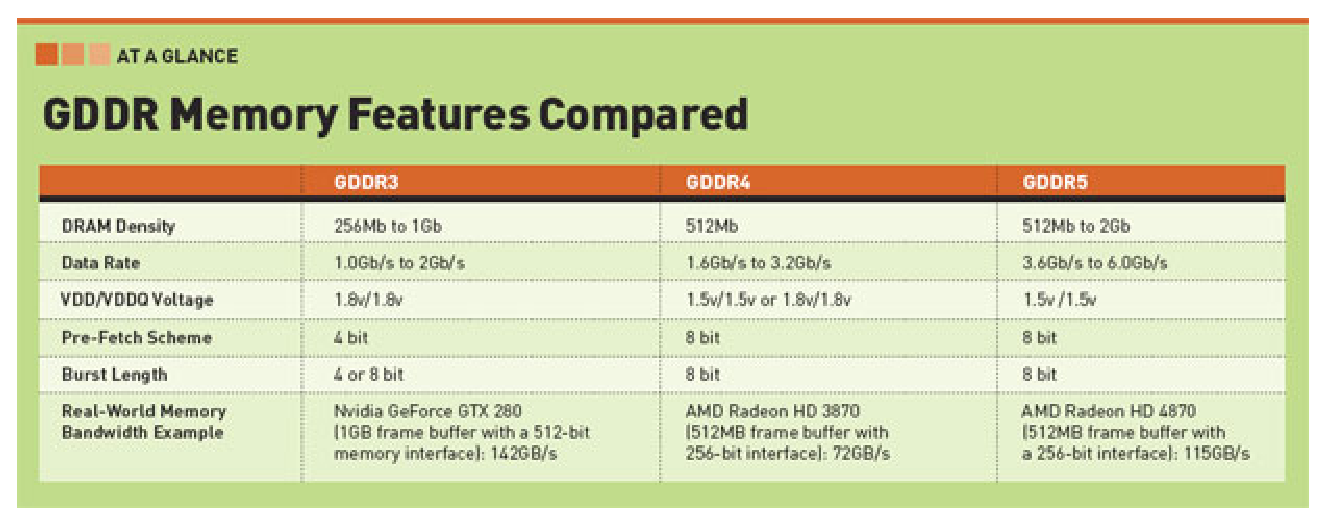
\includegraphics[height=5cm,
    angle=0]{./images/GDDR_mem.eps}}
  \caption{GDDR memory at a glance}
  \label{fig:GDDR_mem}
\end{figure}


Amount of off-chip memory
  \begin{itemize}

  \item Fermi: C2050 has 3GB GDDR5, C2070 has 6GB GDDR5 [NOTE: If
    ECC\footnote{ECC=error correction code, a technique to detect
      error during the storage and transmission of data}
    is enabled, a portion of memory is removed from your usage (12.5\%
    of memory is reserved for ECC checking, so C2050 has only 2.625GB with ECC
    enabled;) and GPU runs a little bit slower.]
  \end{itemize}

  \begin{figure}[hbt]
    \centerline{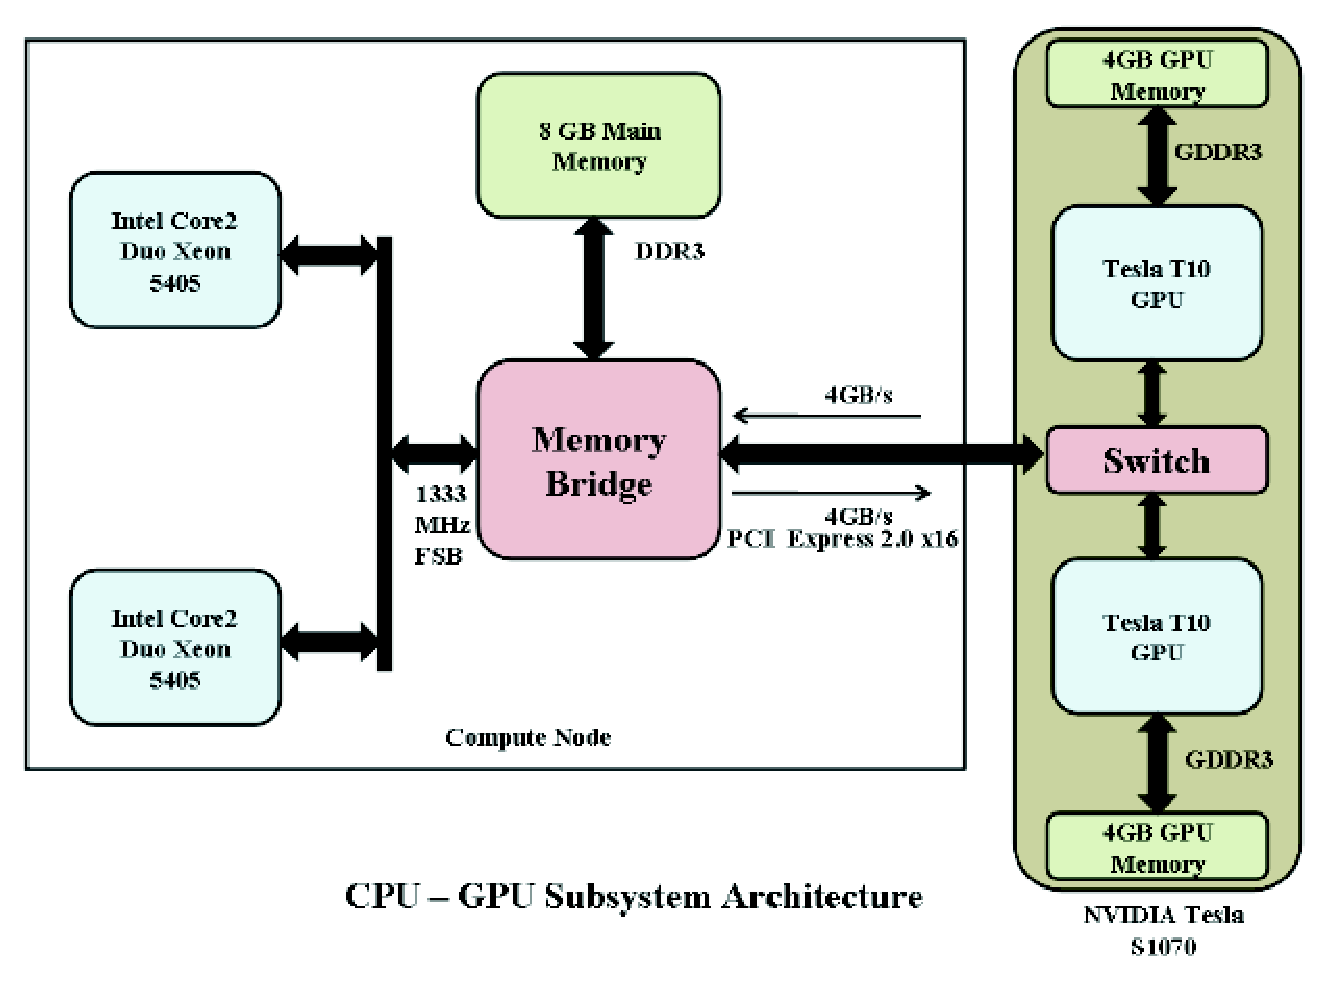
\includegraphics[height=7cm,
      angle=0]{./images/tesla_connect.eps}}
    \caption{Memory access speed: 2 separate dual-core access, each
      compute node access to two Tesla T10 GPU (4 T10 GPUs are packed
      in Tesla S1070)}
    \label{fig:tesla_singlenode}
  \end{figure}

Off-chip memory throughput (theory), as shown in
  Fig.~\ref{fig:tesla_singlenode}
\begin{itemize}

  \item C2050/C2070 access device memory GDDR5: 1152 Gbps = 144 GB/sec (planned
  230 GB/sec, but not able to reach)

  \item
    \textcolor{blue}{M2050/M2070: is C2050/C2070 with an increased in
      memory bandwidth (148 GB/sec)}\footnote{\url{http://www.Nvidia.com/object/product_tesla_M2050_M2070_us.html}}
   
   \item S2050/S2070 ... : $4\times 148=593$ GB/sec
     
  \end{itemize}
  
This value is dependent upon the memory bus bandwidth, the number of memory controller per chip, etc.
  
\subsection{-- HBM2}

Check Sect.\ref{sec:HBM2-RAM}.


\section{Memory Addressing}
 
 In G80 GPUs, an address is defined using 32-bit virtual addressing. To know the
 real address, memory instructions use register plus offset addressing. This
 virtual address is translated into the real address by the MMU.
  
 In GT200 GPUs, an address is defined using 40-bit virtual addressing.
 
 In GF100 GPUs, \ldots
 
 The NVIDIA Fermi GPU architecture, introduced in 2009, implemented a unified GPU address space
spanning the three main GPU memory spaces (thread private local memory, thread block shared
memory, and global memory). This unified address space only applied to GPU memory addressing, and
mainly resulted in simpler compilation by enabling a single load/store instruction and pointer address to
access any of the GPU memory spaces (global, local, or shared memory), rather than different
instructions and pointers for each. This also enabled full C and C++ pointer support, which was a
significant advancement at the time

 
 \subsection{Load/Store}
 
 In order to efficiently access memory, loads and stores must be aligned to
 4Byte boundaries - improperly aligned accesses will result in multiple loads
 or stores being generated by the compiler.  Load instructions across different threads in
a half-warp can be coalesced by the memory controller to reduce the number of
memory transactions.
 
 
 \subsection{Bandwidth information}
 
  \textcolor{red}{We'll describe how to compute the bandwidths from
    these values in Sect.~\ref{sec:hardware-information}}. In 
    \begin{itemize}
      \item GTX 460: 115.2 GBps (256-bit, 1800 MHz)
      \item GTX 460 v2: 96.2 GBps (192-bit, 2004 MHz)
      \item Tesla C2050/C2070: GPU-GDDR5 144 GBps
      \url{http://www.nvidia.com/docs/IO/43395/NV_DS_Tesla_C2050_C2070_jul10_lores.pdf}
      \item GTX 770: 224.3 GB/s (, 7.0 Gbps)
      \url{http://www.nvidia.com/gtx-700-graphics-cards/gtx-770/}
      \item GTX Titan: 288.4 GB/s (384-bit, 6.0 Gbps)
    \end{itemize} 
The number depends on memory clock frequency (i.e. 2 GHz or 7.0 Gbps), memory
interface width (i.e. 256-bit or 512-bit).
    
    
    The major botle-neck is the bandwidth between GPU-DDR3 (dual direction on PCI-e Gen2 x16, DDR3 =
    CPU RAM): 64 Gbps (i.e. 4 Gbps for each direction) [NOTE:
    64Gbps=8GB/sec]. Bandwidth between CPU-DDR3 is about 256 Gbps = 32 GB/sec.
    The connection between CPU-CPU using Intel QuickPath Interconnect (QPI) is
    about 102 Gbps = 12.75 GB/sec. 
    
    Reading and writing data to harddrive is even
    slower:    CPU-SAS/SATA controller is carried out via PCI-e Gen2 x4 = 32 Gbps; and
    SAS/SATA controller - Local Disk is about 8.4 Gbps. On network using
    Infiniband, CPU-Infiniband using PCI-e Gen2 x8 is about 32 Gbps. If we use
    dual Infiniband card per node, the speed would be 2x32=64 Gbps. 

  \begin{framed}
    Due to the low data transfer speed between CPU-GPU, you should
    minimize copying data back and forth. If you need to copy the
    data back to do some computation on CPU, it's sometime better to
    do that directly on GPU to avoid copy data back, even though
    running on GPU is slower than running on CPU.

    If you need to copy the data, it's better to copy a single large
    size batch of data, rather than many small size chunks.
    \textcolor{red}{The recommended size is a chunk not larger than 10MB, and a
    multiple of 64}. Larger than that, we observe a saturation in performance.

    If not overwritten, data on off-chip memory and L2 cache are preserved
    between kernel calls.
  \end{framed}

At SC14, a team of researchers from Argonne National Laboratory and DataDirect
Networks (DDN) moved 64 TB of data in under just 100 minutes using 100 Gbps WAN
connection, i.e. about 16 hours using 10 Gbps. This typically takes 2 days using
10 Gbps connection. They were abled to sustain data transfer rates over 85 Gbps,
with peak at over 90 Gbps (benchmarked using \verb!iperf! tool). They used
\begin{itemize}
  \item Globus GridFTP server
  \item advanced 100G wide-area network
  \item embeded file system and virtual machine capabilities of DDN storage
  controller.
\end{itemize}

The benchmark for disk-to-disk WAN data transfers has a number of challenges,
e.g. the block size that would work well for both disk I/O and network I/O,
selecting the appropriate combination of parallel storage I/O threads and parallel TCP streams
for optimal end-to-end performance.
\footnote{\url{http://www.sciencedaily.com/releases/2014/12/141203124806.htm}}


Comparison between GPU/APU cache and memory latencies:
\url{http://www.sisoftware.net/?d=qa&f=gpu_mem_latency}
 
TOE (TCP Offload Engine) is the network card equivalent to a GPU from a graphic
cards with something like DMA (Direct Memory Access). It allows offloading the
work of the TCp/IP stack to the NIC instead of running through motherboard
front-side bus (FSB) and CPU. 


  REFERENCE:
  \url{http://en.wikipedia.org/wiki/List_of_device_bandwidths}
 
\subsection{-- slowest (network)}


When doing sequential I/O (e.g. media server with video, music or photos) with
multiple disks, the bottleneck is in the gigabit network (those below 10Gbps
network), before reaching the limit of CPU or storage disks.


\subsection{-- slow: persistent storage (harddrive)}

Speed rate (round per minute of the platters) of platter disks:
\begin{itemize}
  \item 5400 and 7200 RPM
  
  With 7200RPM, typical disk-to-buffer data rate is 1030 Mbit/s, i.e. 0.1 GB/s.
  
  Using SATA, e.g. 3.0 Gbit/s SATA, the data rate is about 300 megabyte/s, i.e.
  2.33 GB/s.

  MegaRAID SAS 9300 family of 12Gb/s. 
  
  \item 1200 RPM and as high as 15K RPM.
\end{itemize}

When doing random I/O, the bottleneck is on the platter disks, but SSDs can
easily put the bottleneck back on the gigabit networking. Having said that, some
platter disks can do random I/O very fast (e.g. WD Black drivers, 10K rpm drives
or 15K rpm drives). Short answer is you are generally not bound by CPU/RAM/Bus
until 10Gbps network cards are being used.

{\bf SSD and hybrid SSD}: New solid state hybrid drive (SSHD) technology, that
RPM does not matter. SSHD design is based on identifying frequently used data
and placing it in the SSD or NAND flash portion of the drive.
NAND flash media is very fast, partly because there are no moving parts since
it's made of solid state circuitry with   about 200 MB/s to 1500 MB/s.
\begin{itemize}
  \item 2nd Gen SSHD (based on 7200RPM):
  
  
  \item 3rd Gen SSHD (based on 5000RPM): the technology actually delivers faster
  performance
  
  Western Digital SSHD WD10J31X 1TB SATA 6 Gbps 
\end{itemize}

Fusion-io ioDrive Octal can deliver 6.7 GB/s 



Example: using 5 disks for I/O, it can run more than 3x gigabit speed with
sustained sequential I/O.
\url{http://superuser.com/questions/612429/gigabit-throughput-bound-more-by-cpu-ram-or-disk-io}


\subsection{-- faster: RAM}


NOTE: (933 million hertz * (2 interfaces) * (64 lines/interface) * (2
bits/line-cycle)) = 238,848 Mbit/s, or 29,856 MB/s, or 29.15 GB/s. 

\subsection{-- faster: cache}



\section{Instruction throughputs}
\label{sec:instr-thro-1}

Computational throughput (i.e. number of floating-point operations per
second) - theory speed
  \begin{itemize}
  \item CPU (per core): Intel Nehalem X5365 - 38 GFLOPS
  \item C870: 518 GFLOPS (single-precision), 0 (double)
  \item S870: 2073 GFLOPS (single), 0 (double) 
  \item C1060: 933 GFLOPS (single), 78 GFLOPS
    (double)
  \item S1070: 4147 GFLOPS (single), 345 GFLOPS (double)
  \item C2050/C2070: 1288 (???1030) GFLOPS or 1.03 TFLOPS (single or
    fp32), 515 GFLOPS (double or fp64) (planned: 700 GFLOPS
    (double-precision))
  \item S2050/S2070: 5152 GFLOPS (single), 2060 GFLOPS (double)
  \item AMD Radeon HD 6900: 5.1TFLOPs (single), 1.27TFLOPS (double).
  \item AMD Radeon HD 7970: 3.79 TFLOPS (single), 0.947 TFLOPs (double).
  
  \item Tesla P100 GPU (Pascal): 5.3 TFLOPS of double precision floating point (FP64) performance;
	10.6 TFLOPS of single precision (FP32) performance; 21.2 TFLOPS of half-precision (FP16) performance.  

  \item 
  \end{itemize}

  \begin{framed}
    Issues with memory throughput and computational throughput will be
    targeted in Sect.~\ref{sec:start-point-optim}.
  \end{framed}

\section{Power consumption}
\label{sec:power-consumption}

Power consumption
  \begin{itemize}
  \item Intel X6800
    (2.94GHZ)\footnote{\url{http://blogs.zdnet.com/Ou/?p=273}}:
    160-217 W
  \item Tesla C870: 170W
  \item Tesla C1060: 160-200 W
  \item Fermi : 225W-238W
  \item AMD Radeon HD 7970: 45 W
  \end{itemize}

\subsection{Thermal Design Power (TDP)}
\label{sec:TDP-thermal-design-power}

CPU's Thermal Design Power (TDP) tells how much power is consumed at full load.
Processors using the LGA1155 socket has TDP from 35 watts to 95 watts. 
Core i7-3930K on the LGA2011 socket has TDP 130 watts. 

\url{http://www.pcmag.com/category2/0,2806,794,00.asp}

\section{Costs}
\label{sec:costs}

Cost
\begin{itemize}
\item Intel Nehalem: about 300\$
\item Tesla C870: about 1500\$
\item Tesla C1060: about 1300\$
\item Tesla C2050: about 2500\$
\end{itemize}


\section{Threads}
\label{sec:threads-1}

A thread is an instance of a sequence of code that run as an execution unit,
that means each thread is managed independently by an operating system
scheduler. In most cases, a thread is contained inside a process. Multiple
threads inside a process can share resources (e.g. memory), while one process
can not acces data from another process. Typically, a simple program is a
single-thread process.

On a single processor (one core CPU), multi-tasking or multithreading generally
occurs by time-division multiplexing, i.e. the processor switches between
threads (known as {\it context switching}). Due to the resource limition (e.g.
number of general-purpose registers), context switching from one thread
in one process to a thread in another process is expensive in the sense that
resources need to be saved, and restored.

Thread switching on GPU, on the other hand, is cheap, as resources (registers,
shared memory) are allocated for each thread in advances. So, there's no need to
save and restored data in registers, shared memory, etc.  

Techniques to run multiple threads simultaneously on a single CPU core
include Intel hyper-threading technology HTT (Pentium 4 Desktop and Xeon server in
2002). Here, the operating system address two virtual or logical CPU cores so
that the operating system can schedule two processes for each CPU core which
can give some performance gain for multi-threaded single-process code.
The technology requires the Operating System to be designed and optomized for
HTT. Hyper-threading means multiple-logical cores in one physical core. It's a
marketing term for {\bf Switch-on-Event MultiThreading} (on Itanium) or {\bf
Simultaneous MultiThreading} (on x86). 

Threads
\begin{itemize}  
  \item CPU: 4 quad-core CPUs can run 16 threads in parallel (or 32 if
    HyperThreading is supported). One UltraSPARC T2 CPU core each one can handle
    8 threads concurrently, i.e. 64-concurent thread for a 8-core CPU.
    UltraSPARKC T3 with 16-CPU cores can handle 128-concurent threads. 
    
  \item Nvidia C870 can load 768 threads at the same time per SM
    $\rightarrow$ 12,288 threads can be loaded simultaneously per chip
  \item Nvidia Tesla C1060 can load 1024 threads per SM $\rightarrow$ 30,720
    threads can be loaded simultaneously per chip
  \item Nvidia Fermi C2050/C2070 can have 1536 threads per SM $\rightarrow$
  21504 threads can be loaded simultaneously per chip. 
\end{itemize}

The number of threads to be loaded in GPU in a real application is indeed  lower
than the maximum possible value. The reason is that users need to  balance with
other limitations to achieve a high performance, e.g.   registers usage
(Sect.\ref{sec:reg}), shared memory usage 
(Sect.\ref{sec:shared-memory-bank})...  In essence, number of threads is
unlikely to be the bottleneck in GPU  execution. This is the reason why Fermi,
rather than trying to increase the  number of maximum parallel threads, was
designed to improve other features (e.g. cache). Fermi has a lower number of
maximum threads to be loaded compared to  Tesla.

\begin{framed}
A thread is often described in terms of weight (heavy-weight, medium-weight or
light-weight), meaning how much contextual information (e.g. local data
values, hardware registers, user-level stack, etc.) must be saved for a given
thread so that resources are free for other processes to use, and also the
offline process can be restored and continued execution by the processor later.
A UNIX process is heavy-weight. A user-level thread is light-weight.
\textcolor{blue}{In CPU, thread switching is per single-thread}.

Threads in GPU are light-weight. Context switches between GPU threads are
extremely lightweight. The reason is that the resources are statistically
allocated and assigned to each thread until it completes. Thousands of threads
are queued up. \textcolor{blue}{GPU threads are launched and switched in
groups of threads (called {\bf warps})}. The exact number of threads per warp
vary from one generation of GPU to another. 
\end{framed}


\subsection{Core and Threads}
\label{sec:core-thread}

All AMD-based CPU accepts one thread per core. Example: a 4-core AMD CPU limit 4
threads in an application. Some Intel CPUs use {\it
Hyper-Threading} that mimics multiple threads within cores, i.e. two threads per
core. An Intel quad-core model can run 8 threads in the same application, which
can bring some performance gain, but it is not necessary twice the speed. 

Hyper-Threading simulates some degrees of overlapping in executing two or more
independent instructions. Intel uses additional registers to overlap two
instruction stream to achieve about 30\% performance gain. To take advantage of
multi-core or hyper-threading of single-core, a software must be written in
multithread (Pthread, OpenMP).

It's important to know about {\bf clock speed}
(Sect.\ref{sec:clock-cycles-speeds}). 


\section{GPGPU (General-Purpose GPU): unified-architectures}
\label{sec:gpu-unified-architecture}

Programs, i.e. binary files, that can run on graphics card are traditionally
called {\bf shaders}, each executable binary is supposed to handle one stage of
the rendering pipeline, Fig.\ref{fig:graph_pipeline_2} as these binaries are
supposed to do a particular shading effect on the input which is typically a
graphic image.

The term {\it shader} is also refer to the GPU core in charge of doing shading
(or coloring)) - Sect.\ref{sec:cores} - and data need to be interpreted as
graphical data which requires the programmers to have a certain level of
understanding of graphical programming. Programming languages for GPU designed
to compile the code, into binary files that run code on GPU, is not easy for
non-graphical programmers.

Folks eventually figured out how to use these shaders to do things unrelated to
graphics, or at least unrelated to the fixed-function rendering pipeline. The
GPUs gained support for more and more general-purpose programming and the
graphics APIs eventually gained support for "compute shaders" that live outside
the rendering pipeline.

In opposite to Shaders (Sect.\ref{sec:shader}) which put a 'shader' program into
one category that falls into one of the stage of the graphics pipeline, CUDA
programming model is not restricted to a specific step of the rendering
pipeline. CUDA (and the many, many related technologies) is essentially just a
way to run compute shaders without the graphics API and without requiring a
particular language. GPU with this capabilities is known as {\bf unified-architecture}.

\begin{mdframed}

Previously, some GPU core are designed for pixel shading, and some are designed
for vertice shading, or geometry shading.  There is a fraction of GPU cores for
running vertice shading, and some other fraction of GPU cores for geometry
shading, for example. One GPU core cannot do both. So balancing the number of
cores for each tasks, at manufacturing stage, is important.

The unified architecture means that all GPU core are identical and they can do
the same thing (vertex, pixel, geometry and compute kernels).

\end{mdframed}

Recently, the shift in GPU architecture and the extension of the GPU instruction
set have enable GPU to handle intensive parallel computational applications,
i.e. running 'compute shaders' for more generalized applications.
Even though ATI was the first to develop the unified architecture, it is Nvidia
that bring GPGPU to the hype - with the name {\bf Compute Unified Device
Architecture} (CUDA). 

However, conventional programming languages are designed to compile the code
running on CPU.

CUDA programming model is designed to run on Nvidia's GPU with CUDA architecture
(Chap.\ref{chap:cuda-gpu-architecture}). CUDA programs are compiled into PTX
(NVIDIA's analoque to x86 assembly for the GPU, though a bit more abstract to
remain compatible with GPU revisions) and come be compiled from any number of
languages, be it C++, Rust, (variants of) Python, or so on. These kinds of
programs could be compiled into HLSL or GLSL as well, but this is often a lot
harder to develop and debug.


\chapter{CUDA Architecture: Tesla 1 and Tesla 2}
\label{chap:cuda-gpu-architecture}

Even though ATI/AMD was the first to develop the unified architecture, it is Nvidia
that bring GPGPU to the hype - with the name {\bf Compute Unified Device
Architecture} (CUDA).

\section{Compute Unified Device Architecture (CUDA)}
\label{sec:gpu-unif-arch}

Along with developing the GPU's unified-architecture, Nvidia also provides a
programming model on this new GPU architecture. They are both called CUDA
(Compute-Unified Device Architecture).

The GPU core is now called {\bf CUDA core} or scalar processor (SP) -
Sect.\ref{sec:stre-proc-sp}.

 
Full performance is achieved irrespective of input vector size, e.g. scalar data
(Z-buffer), 3-component vectors (3D coordinates), 4-component vectors (RGBA
color).

Nvidia's unified approach started with G80 chips in 2006
(Sect.\ref{sec:g80g92-architecture}).

In addition to CUDA architecture, in 2007 Nvidia present the first programming
model to interface with GPU - called CUDA as well
(Sect.\ref{sec:cuda-progr-model}).

As CUDA programming model is designed for general purpose programming on GPU,
the first GPU device targeting to high-performance computing was also created, named
{\bf Tesla}.
\begin{itemize}
\item Tesla 1 is C870
\item Tesla 2 is C1060
\item Tesla 3 (widely known as Fermi) is C2050 which use GF100 chip.

NOTE: There are some pitfalls with GF100 (high heat, large die size). Later,
Nvidia developed some revision versions of GF100, like GF104/GF106/GF108. The
main change is the switching from 32SP per SM to 48SP per SM (check more detail
in Sect.\ref{sec:stre-mult-sm}).

\item Tesla 4 (Kepler) that use GK110 chip.
\end{itemize}


\begin{framed}
  Tesla 1 and 2 are based on G80/G92 and GTX200, respectively. As
  G80/92 and GT200 were designed especially for graphical
  applications, they have texture caches which is extensively used by
  GPU. That's why C870 and C1060, though don't have VGA/DVI output,
  still have texture cache.
\end{framed}

Tesla 1/2 has three level hierarchies:
\begin{itemize}
\item level 1: a GPU chip is divided into a number of TPCs (Thread
  Processing Clusters - in computing mode, Texture Processing Cluster
  - in graphics mode)
\item level 2: each TPC is a group of some SMs (streaming
  multiprocessors), adding with L1 texture cache (serves as a memory
  pipeline for the SMs in the group) and some logic control units.
\item level 3: each SM is a group of 8 SPs + some special units.
\end{itemize}
In the coming sections we will describe in detail the structure of
each level. A roughly comparison between GPU and CPU is shown in
Fig.~\ref{fig:g80_gt200_niagra}. 

\begin{framed}
  CPUs are multi-cores, yet GPUs are many-cores.  The concept of
  ``cores'' (ALUs (arithmetical and logical unit) and FPUs
  (floating-point units) - the real processing units that act on
  pixel/vertex/general data) in GPUs is slightly limited, as lack a
  complete front-end that can fetch instructions, and schedule
  instructions independently. GPU cores are known as [scalar]
  processors (SP) or {\it shaders} or {\it thread processor}.  Nvidia
  took a bunch of SPs, gave them a L1 texture cache, some shared
  memory and 2 special functional units, and called the whole
  construct as streaming multiprocessor (SMs).
\end{framed}


% \subsection{CUDA architecture}
% \label{sec:cuda-arch-cuda}


\subsection{Scalar Processor or Streaming Processor (SP)}
\label{sec:stre-proc-sp}

\textcolor{red}{In the context of CUDA, any shaders are now called {\it scalar
(streaming) processors (SP)} or thread processor} (as each SP processes an
instruction from a single thread). In AMD/ATI context, SP is named as an SIMD
(single-instruction multiple data) unit. In GPU, it processes and render pixel
(voxel) data in the same way for every pixel (voxel), but with different data,
which explains the term single-instruction multiple data. In Fermi, SP is now
called {\bf CUDA core}.


Each scalar processor (SP) or GPU core, however, lacks a complete front-end that
can fetch and schedule instructions independently.  Thus, SP is most closely
corresponding to an issue pipeline or a modern multi-threaded CPU.

\subsection{-- G80/92 SP}

Nvidia's {\bf G80/92} GPU: A single SP can do either
\begin{itemize}
\item 1 MAD FP32s, 
\item 1 ADD INT32s, 
\item 1 MUL INT24s
\end{itemize}

In multiplication operations, first-generation SP supports only 24-bit
scalar multiply-add (MAD) unit, which execute mostly IEEE compliant
single-precision FP and integer 32-bit ALU warp instruction
\textcolor{red}{in 4 cycles} (4 fast clock cycles or shader
clock)\footnote{32-bit precision is performed in emulation mode; thus
  slow down the performance. To use 24-bit computing, compile with
  -use-fast-math if accuracy is not critical}.

\subsection{-- GT200 SP}

{\bf With GT200}:
\begin{itemize}
\item Integer arithmetic operations are still 24-bit in hardware, and
  32-bit need software emulation (i.e. run slow)
\end{itemize}

\subsection{-- Fermi redesigned SP}
\label{sec:SP-Fermi}

{\bf With Fermi}: has newly designed SP with (fully pipelined) integer (INT)
unit and floating-point (FP) unit.
    
    
\begin{itemize}
  
  \item   support full 32-bit operations for all instructions, rather than
  24-bit as in GT200.
    
  All arithmetic operations are 32-bit in hardware. Integer ALU is
  also optimized to efficiently support 64-bit and extended precision
  operations (see Sect.~\ref{sec:special-instructions}).
  
  \item   new FMAD unit: each SP stills does single-precision operations;
  but 
    \textcolor{red}{two SPs can do 64-bit operations, so we don't need
      a separate 64-bit MAD unit}.
      
 Thus, new FMAD can do both single and double-precision operations, i.e. two
 32-bit ALUs can now function as one double-precision unit, thus C2050 has
 16x14=224 double-precision units, and is 1/2 slower than 32-bit
  FP (used to be 1/8 in GT 200, and 1/5 in AMD's).
       
 \item support full IEEE 754-2008 standard.

    Using IEEE754-2008 standard, all multiply/add arithmetic
    operations are fused to enhanced the precision,
    Fig.~\ref{fig:FMAD}.

\end{itemize}

    \begin{figure}[hbt]
      \centerline{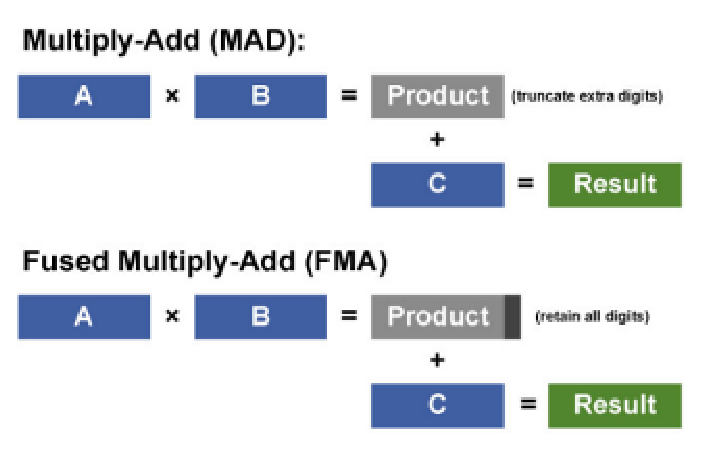
\includegraphics[height=4cm,
        angle=0]{./images/FMAD.eps}}
      \caption{Fused Muliply-Add (FMAD) in Fermi}
      \label{fig:FMAD}
    \end{figure}

\subsection{Streaming Multiprocessor (SM)}
\label{sec:stre-mult-sm}

{\bf SM configuration}: Each SM is composed of a number of SPs and some
supporting units. A streaming multiprocess (SM) is a complete computing unit
with components like instruction fetch and instruction dispatcher.

\begin{enumerate}
  \item Tesla-1 SM	 - Sect.\ref{sec:SM-Tesla-1}
  
  \item Tesla-2 SM - Sect.\ref{sec:SM-Tesla-2}
  
  \item 
\end{enumerate}

\subsection{-- Tesla-1 (G80/G92) SM}
\label{sec:SM-Tesla-1}

Tesla 1st gen: with 128 single-precision SPs (no double-precision core)
  
Each SM is composed of 8 SPs + 2 SFUs + 1 MT issue + 1 I-cache + 1 C-cache +
16KB shared-memory + 16KB L1 texture-cache + 8K 32-bit registers + 1 WARP scheduler
    
\begin{itemize}
  \item  $\rightarrow$ the chip has total 16 SMs.
  % \item SPs in this generation are limited to 24-bit precision for
  %   multiplications. 

  \item A SFU unit are indeed a cluster of several units that can
    handle unusual and exceptional operations in GPU,
    e.g. transcendental functions (sin(), cos(), reciprocal,
    square-root, exp()...), interpolation for parameter blending. For
    a list of supported special instructions, read
    Sect.~\ref{sec:special-instructions}. Each SFU executes one
    instruction per thread, per clock. So, a warp (32 threads)
    executes over 16 clocks.  Instructions which are natively executed
    by the SFU have \textcolor{red}{a 16 clock cycle latency}, while
    more complicated functions, e.g. square roots or exponentiation
    are synthesized by the compiler using a combination of
    instructions and take \textcolor{red}{32 clock cycles or longer}
    to execute. SFU hardware for interpolations include several 32-bit
    FP multiply units (FMUL), which can be issued separately for
    multiply instruction.

    SFU is physically implemented by 2 execution units: each one
    services 4 of the 8 execution pipelines in the SM; and multiply
    instructions issued to the SFU in the same
    \textcolor{red}{4 clock cycles} as in the FMAD unit.

  \end{itemize}

\subsection{-- Tesla-2 (GT200) SM}
\label{sec:SM-Tesla-2}

Tesla 2nd gen: with 240 single-precision SPs.

This is known as the second-generation SM, Fig.~\ref{fig:SM}.
Each SM is is composed of 8 SPs + 2 SFUs + 1 MT issue + 1 I-cache
+ 1 C-cache + 24KB shared-memory + 24KB L1 texture cache + 1
64-bit FMAD unit + 16K 32-bit registers + 1 WARP scheduler, as
shown in Fig.~\ref{fig:gt200_sm}, $\rightarrow$ total 30 SMs.
    
\begin{itemize}
  \item A new unit - the double precision fused-multiply-add (FMAD)
    unit (FP64-unit) has been added which supports standard IEEE 754-1985
    behavior, with full speed de-normal handling and classic 64 bit integer
    arithmetic. 
    
In GT200, a brand new 64-bit FMAD shared by the entire SM for integer
and floating point computation that relies on the new support 64-bit
register files. This is also a double-precision FMA unit (support
standard IEEE 754-1985), with full speed de-normal handling and
classic 64-bit integer arithmetic. 

In total, GT200 has 30 FP64 units.
\end{itemize}

\begin{figure}[hbt]
  \centerline{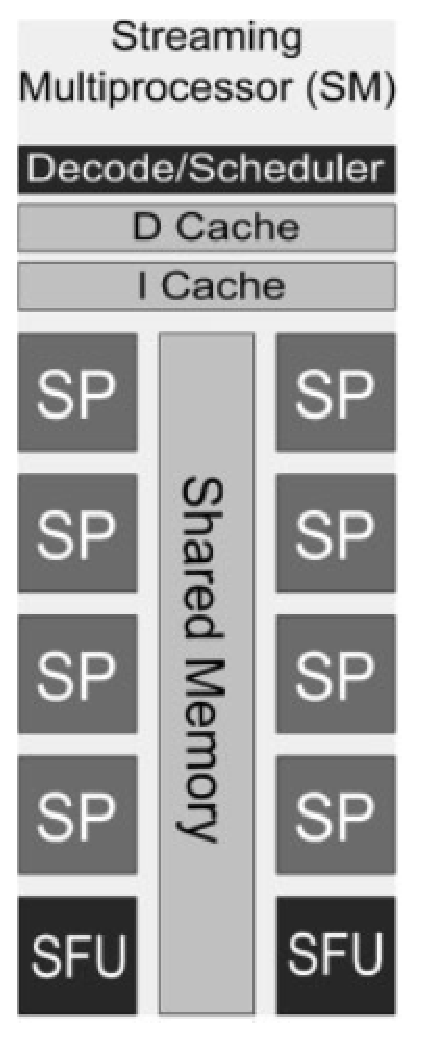
\includegraphics[height=5cm,
    angle=0]{./images/SM_GT200.eps}}
 \caption{SM of GT200}
\label{fig:SM}
\end{figure}


\begin{framed}
  FMAD performs a fused multiply-add with a single rounding on the
  result, i.e. enabling more accurate result (especially on iterative
  algorithms).  Even though using FMAD improve the accuracy, it
  decreases the performance, as the number of FMAD units is 1/4 of
  double-precision units in Fermi.  In GT200, every 8 SPs has one
  separate double-precision core, then using double-precision
  computation may decrease the performance by a factor of 8 (to be
  explained in detail in Sect.~\ref{sec:cuda-apis}.
\end{framed}

\subsection{-- Fermi (GF100) SM}
\label{sec:SM-Fermi}

Fermi: use GF100 chip (planned: 512) with 448 single-precision SPs due to design
limitations. \textcolor{red}{This is known as the third-generation SM which has
a lot of innovations}. 
\begin{enumerate}
  \item First is the addition of a Texture Unit which previously
is not part of an SM.
  
  \item  In earlier Tesla GPU, a SM doesn't have cache, which is an essential
  component
in modern CPU. In Fermi GPU, a SM have both shared memory and L1/L2 cache.

   \item implemented a unified GPU address space spanning the three main GPU
   memory spaces (thread private local memory, thread block shared memory, and
   global memory). 
   
This unified address space, however, only applied to GPU memory addressing, and
mainly resulted in simpler compilation by enabling a single load/store
instruction and pointer address to access any of the GPU memory spaces (global,
local, or shared memory), rather than different instructions and pointers for
each. This also enabled full C and C++ pointer support, which was a significant
advancement at the time.
\end{enumerate}

That's why Fermi GPU is considered as the most complete GPU design in that its
SM is most similar to a CPU. 

 \begin{framed}
    
    Rather than at TPC level, 4 TEX units now resides within each SM
    and is clocked at 1/2 the speed of CUDA cores. However, this speed is 
    still higher
    than those in GT200.
    % Thus, we no longer need a separate 64-bit arithmetic unit.
  \end{framed}  

Each SM is composed of 
\begin{itemize}
  \item 32 redesigned SPs - Sect.\ref{sec:SP-Fermi}

Every SM now has 32, rather than 8 SPs. 
        
  \item 4 SFUs 

 With 4 SFU units,
    \textcolor{red}{a warp execute over 8 clock cycles}. The SFU
    pipeline is decoupled from the dispatch unit, allowing the
    dispatch unit to issue to other execution units while the SFU is
    occupied.

  \item 1 MT issue 

  \item 1 I-cache 
  
  \item  1 uniform-cache (replacement for C-cache) 
  
  \item 64KB shared-memory/L1 cache +
\textcolor{red}{12KB Texture-cache} + 32K 32-bit registers 

New L1 cache/shared-memory configuration allows compiler to
    manage between 16/48 (suitable for graphics application) and 48/16
    (suitable for compute apps), Fig.~\ref{fig:L1_L2}.
    \textcolor{red}{NOTE: The setting is discussed in Sect.~\ref{sec:shared-memory-cache}}.

L1 cache is to store data only for that SM, but share-memory cache is shared
between all SMs. So, depending on your application (whether you want to share
much data between SM or not), you can adjust the amount of L1/share-memory to
match the application's demand. The default is (see next).

  \item 2 WARP schedulers + 2 I-Dispatch Units 
 
  Third generation SMs, with 2 warp-schedulers, can process 2 warps
    at the same time. With 32 SPs per SM, each warp uses 16 SPs, given
    that 32-bit operations are used. If threads use 64-bit operations,
    only a single instruction can be issued as two 32-bit units will
    handle a single 64-bit operation.  

 2 (dual) WARP schedulers + 2 Instruction Dispatch Units allow
    2 warps to be executed concurrently. So, for each warp, an
    instruction is issued to a group of 16 cores, 16 LD/ST units,
    or the 4 SFUs units.
\begin{figure}[hbt]
  \centerline{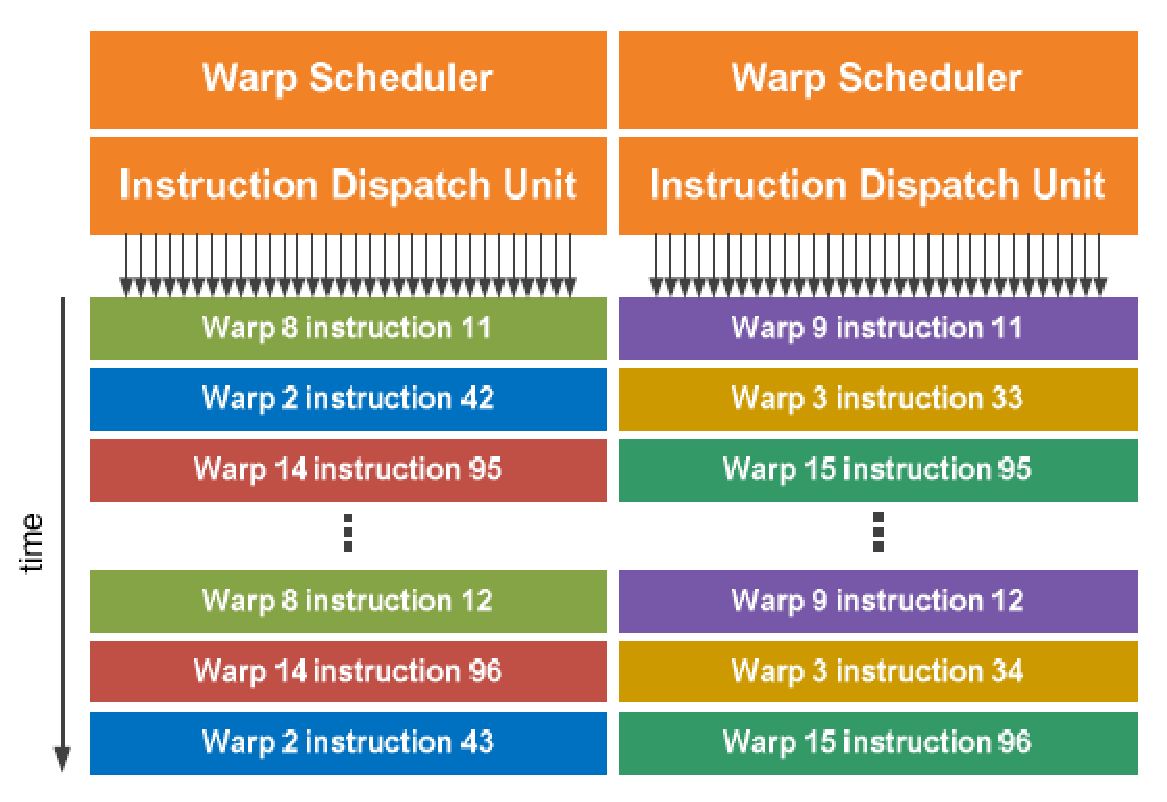
\includegraphics[height=5cm,
    angle=0]{./images/dual_warp_scheduler.eps}}
\caption{Fermi's dual-warp scheduler}
\label{fig:dual_warp_scheduler}
\end{figure}
As shown in Fig.~\ref{fig:dual_warp_scheduler}, the dual-warp
scheduler select 2 warps (to be active), issue one instruction to each
warp. As inter-warp threads are independent, using dual-warp mechanism
can achieves near-peak performance. However, double-precision and
special-purpose unit (SPU) operations (like exp(), sin()...) do not
support dual-dispatch with any other operations.
\textcolor{blue}{Others instructions can be dual-issued (e.g. two
  integer instructions, two floating instructions, or a mix of
  integer, floating point, load, store, and SFU instructions).}
 
  \item 4 TEX units + 1 PolyMorph Engine + 16 load/store (LD/ST) units.

TEX units run at half of the shader clock speed (NOTE: 1/2 shader clock
  speed = core clock). 
  
NOTE: TEX units in GT200 run at the same speed at graphics
  core clock, Fig.~\ref{fig:texture_performance}.

    \begin{figure}[hbt]
      \centerline{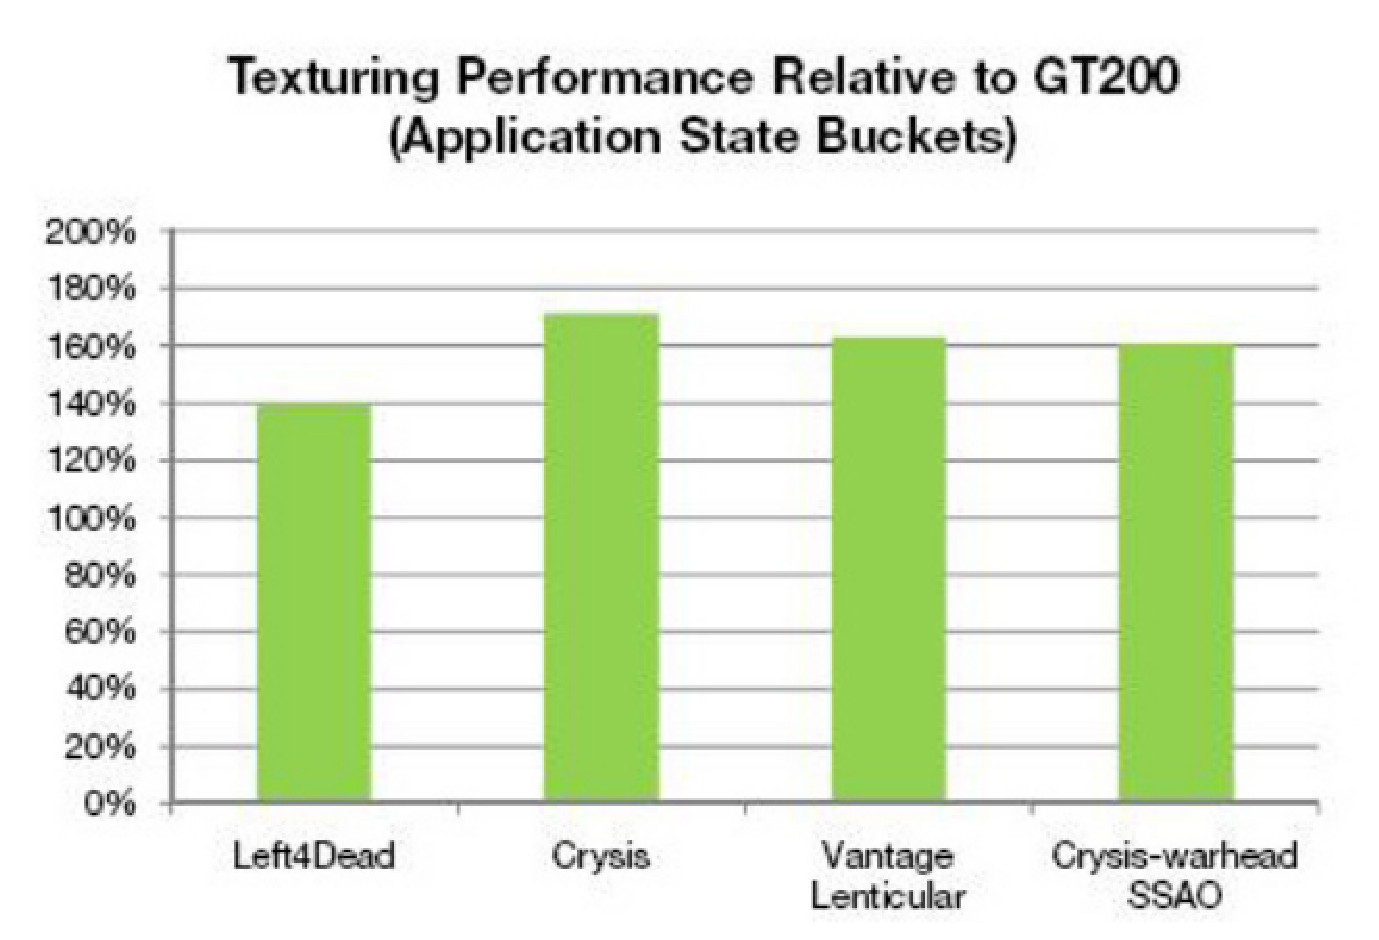
\includegraphics[height=5cm,
        angle=0]{./images/texture_perf.eps}}
      \caption{Texture performance in some applications (GF100 vs. GT200)}
      \label{fig:texture_performance}
    \end{figure}

\end{itemize}


\begin{figure}[hbt]
  \centerline{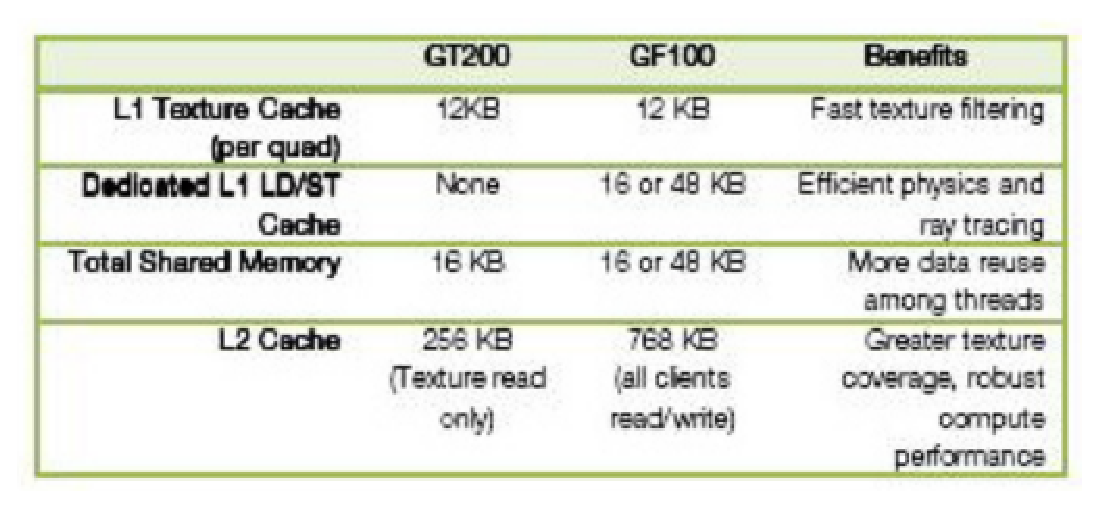
\includegraphics[height=4cm,
    angle=0]{./images/L1_L2_cache.eps}}
  \caption{L1 and L2 cache (NOTE: L2 cache is at chip level which
    means it's shared by all SMs and is particularly useful when all
    SMs need to access the same data). In GT200, L2 cache is indeed L2
    texture cache as it is dedicated to texture read only (CUDA
    Fortran 2010 doesn't support reading texture cache)}
\label{fig:L1_L2}
\end{figure}

\subsection{-- Kepler (GK10) SMX}
\label{sec:SM-Kepler}
\label{sec:Kepler_SMX}
  
Kepler (CC 3.0): use GK10 chip 

Most of the key hardware units for graphics processing reside in the SM.
A major change in Kepler-based GPU is the concept of {\bf SMX} (Shader
Multiprocessor, Shader Multiprocessing Engine), rather than using SM (streaming
multiprocessor), Fig.\ref{fig:Kepler_SMX}. Each SMX has


Each SM now has 
\begin{itemize}
   \item 192 SP (CUDA core for arithmetic operations), 
   
   \item 32 special function units (SFU) for handling single-precision floating-point
   transcendental functions, 
   
   
   \item 4 WARP schedulers.
 
 Each WARP scheduler can issue 2 independent (single-precision)
   instructions of a time (or one double-precision instruction).
   \textcolor{red}{SM is now 6x more SP and SFU}, but 2x more WARP scheduler.
   Maybe they see that the overal latency for each instruction is large so it's
   better to launch more instructions at once to mask the latency.
   
   With 4 WARP scheduler, Kepler K10 can executes 8 (single-precision)
   instructions from 4 different warps at a time. 
   
   \item L1 cache 
 \end{itemize}
   
\begin{figure}[hbt]
\centerline{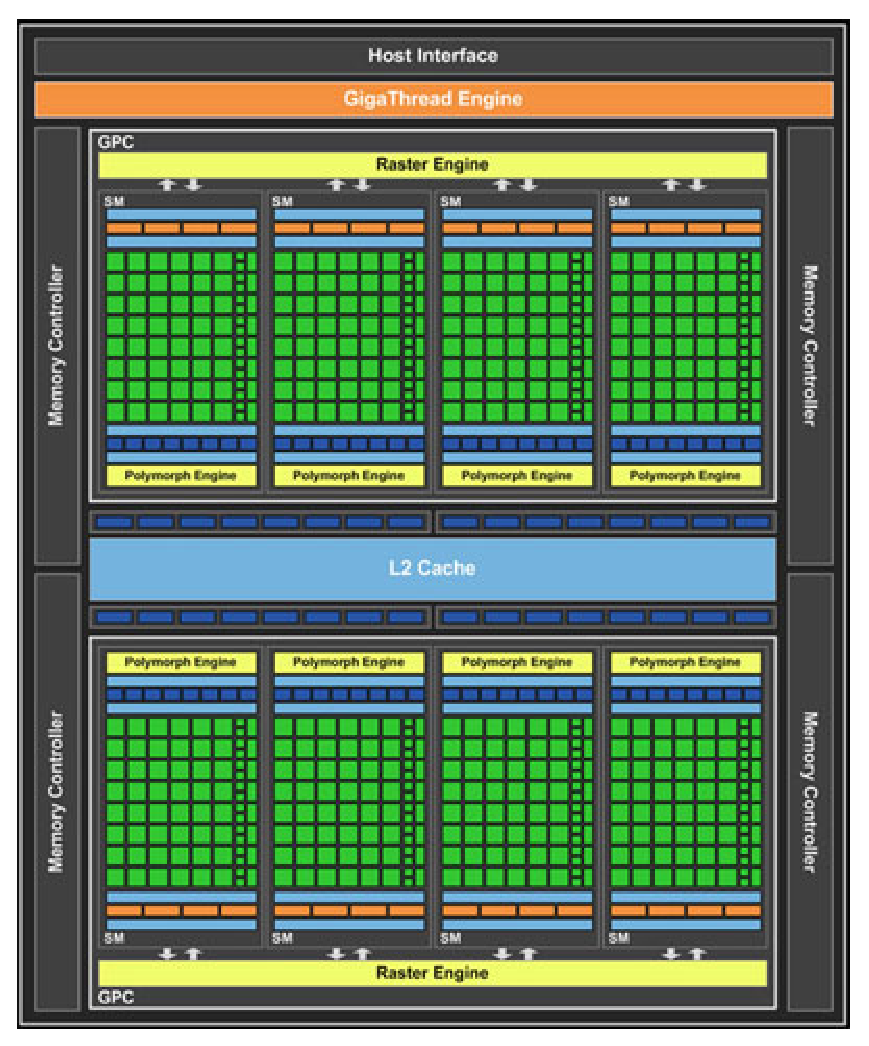
\includegraphics[height=7cm,angle=0]{./images/GF104.eps}
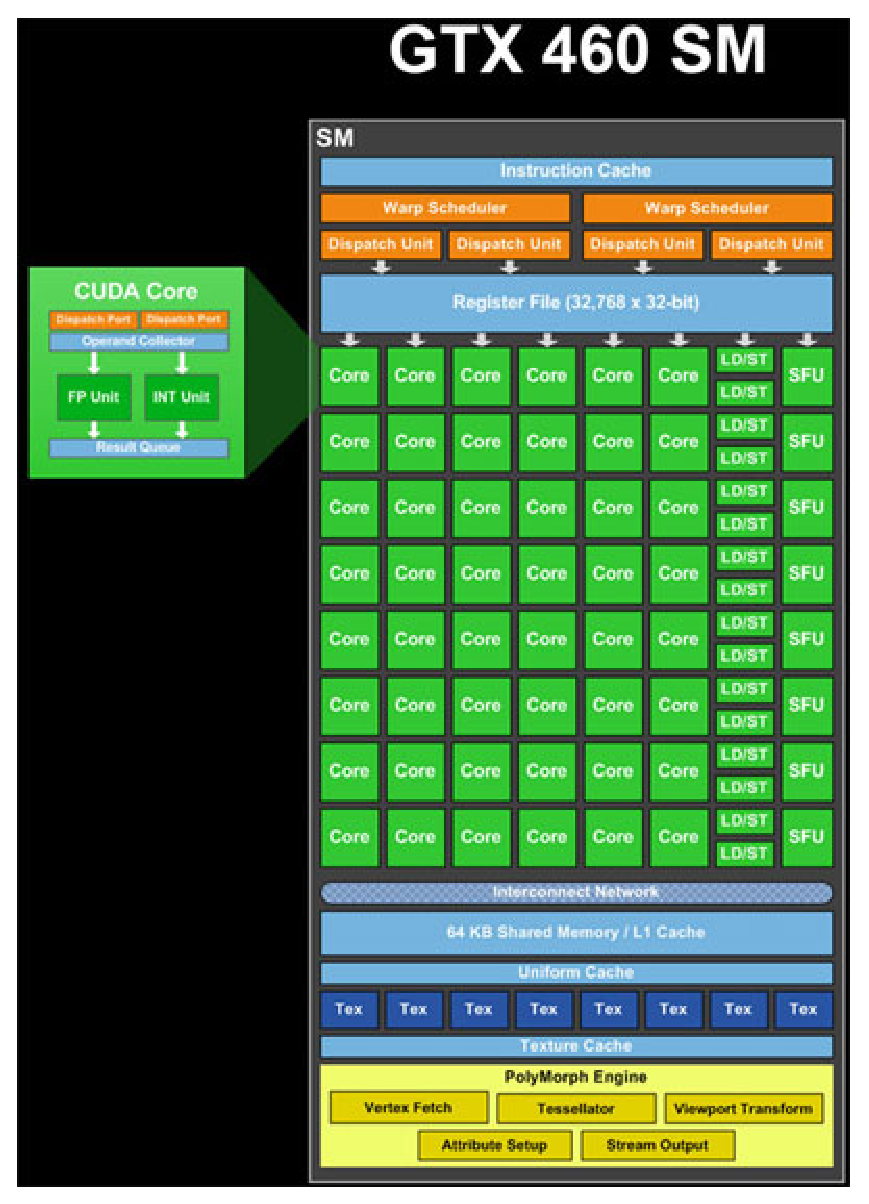
\includegraphics[height=5cm,angle=0]{./images/GF104_SM.eps}}
\caption{GTX 460 SM based on GF104. A GTC in GF104 has 48 SPs}
\label{fig:GF104}
\end{figure}

\begin{framed}
  SM can work with shaders of any types (vertex, pixel, geometric),
  and process them using its scalar processors.  Each SM is loosely
  considered as a modern microprocessors with 8-wide SIMDs. The
  front-end of each SM is (1) an instruction fetch, (2) decode and
  issue logic, (3) execution units. Thus, in the context of OpenCL, SM
  is called {\bf compute unit}.
\end{framed}

\subsection{-- Maxwell (GM200) SM}
\label{sec:SM-Maxwell}


\subsection{-- Pascal SM}
\label{sec:SM-Pascal}

Each SM has 64 CUDA Cores and four texture units (TEX units).

\begin{itemize}
  \item   64 single-precision (FP32) CUDA Cores

 In contrast, the Maxwell and Kepler SMs had 128 and 192 FP32 CUDA Cores,
 respectively.
 
 While a GP100 SM has half the total number of CUDA Cores of a Maxwell SM, it
 maintains the same register file size and supports similar occupancy of warps
 and thread blocks.

  
  \item 
\end{itemize}

\subsection{Texture Processing Cluster (TPC)}
\label{sec:TPC-TextureProcessingCluster}


{\bf Texture Processing Cluster (TPC) configurations}: All texture functions are
processed inside a TPC. A single GPU chip is a configuration of TPC.
\begin{enumerate}
  \item Tesla-1 TPC
  \item Tesla-2 TPC
\end{enumerate}

Since Kepler, TPC is replaced by GPC (Sect.\ref{sec:GPC}).


\subsection{-- Tesla-1 TPC}

Tesla 1st gen:     have 8 TPCs.

Each TPC is composed of 
\begin{itemize}
  \item 2 SMs 
  
  \item 1 TEX engine (texture unit) 
  
  \item 1 geometry controller (GC) 

  \item 1 SM controller (SMC). 
\end{itemize}


\subsection{-- Tesla-2 (GT200) TPC}

Tesla 2nd gen: have 10 TPCs.

Each TPC is composed of
  \begin{itemize}
  \item 3 SMs 

  \item 1 TEX engine (which contains 8
    texture filtering units)
    
  \item 1 geometry controller (GC) 
  
  \item 1 SM controller (SMC). 
\end{itemize}

\subsection{-- Pascal TPC}
\label{sec:TPC-Pascal}


Each TPC of GP100 has two SMs.



\subsection{TPC to GPC}
\label{sec:tpc-gpc}
\label{sec:GPC}

GT200 has 3 levels (excluding SP): GPU, TPC and the SM. This is a complex
structure and Nvidia decided to rethink it completely in Kepler GPU. 

With the Texture Unit moved into the SM in Kepler GPU, there's no need to use
TPC. Instead, a new concept is developed called GPC ({\bf Graphics Processing
Cluster}) which is a considered as a self-contained GPU.

Most GPU's graphics functions are performed inside the GPC. In GT200, the whole
chip has only a single {\it Raster Engine}. Now, in Fermi, each GPC is equipped
with a Raster Engine, which allows it to function as a self-contained GPU.  This
is the reason the name was given.

\subsection{-- Fermi (GF100) GPC}
    
In Fermi, each GPC has a 
\begin{enumerate}
  \item one Raster Engine: triangle setup, rasterization, z-cull
  \item four SMs
  
The size of SM in Fermi (32 SPs (GF100) or 48 SPs (GF104)) is different from
previous version of GPUs (8 SPs); 

NOTE: some components (e.g. TEX units...) are moved to the SM level (read
Sect.~\ref{sec:stre-mult-sm}), Fig.\ref{fig:Fermi_GPC}.

\end{enumerate}


Ideally, a Fermi card has 4 full GPCs. However, due to the limitation of 40nm
architecture, in the last GPC of GF100 chip, two SMs are disabled. From GF110
chip, all four GPCs has the full 4 SMs.

With 4 GPCs, a Fermi chip have 16 SMs. However, two are disabled, and total 14
SMs are enabled. \footnote{ Tesla 3rd gen was expected to have 512 cores (with
16 SMs); yet due to limitation of 40nm architecture, current Fermi has only 14
SMs enabled}.

\begin{figure}[hbt]
  \centerline{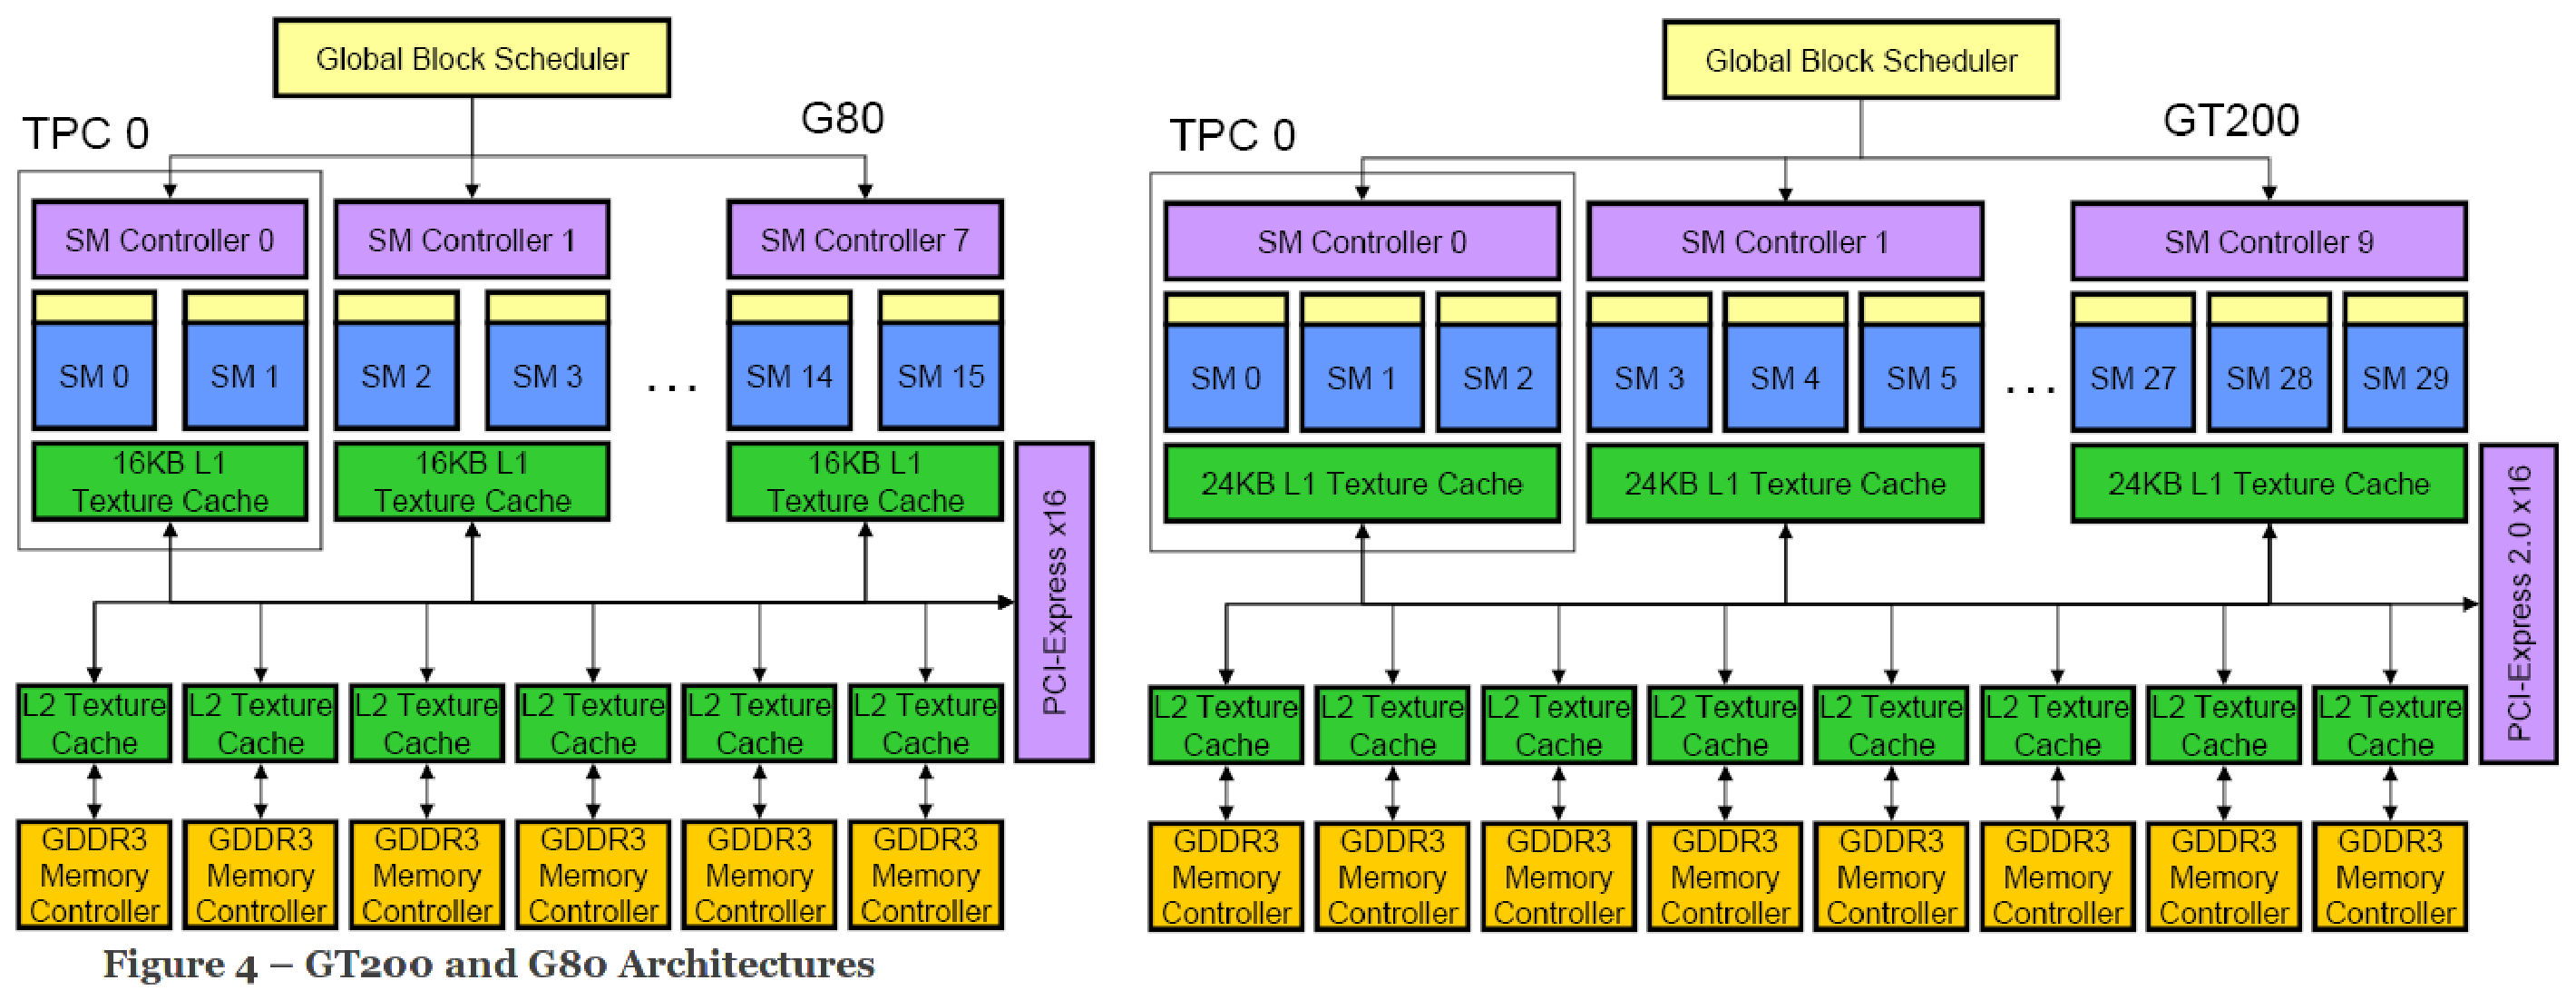
\includegraphics[height=5cm,
    angle=0]{./images/g80_gt200.eps}}
  \caption{G80 and GT200 architectures}
  \label{fig:g80_gt200}
\end{figure}

\begin{framed}

GF104:  While GF100 has 4 GPCs (each with 4 SMs, each SM with 32 SPs); GF104 has
2 GPCs, each also with 4 SMs; yet now \textcolor{red}{each SM with
  48 SPs}, Fig.\ref{fig:GF104}. GF104 has one SM disabled; so it has 7*48= 336
  SPs totally. To balance the increase in SPs/SM, GF104 has double the number of
  instruction dispatch (to 4), and the number of texture units (to 8) per SP.
  So, it supports higher concentration of texture performance than shader
  performance compared to GF100.
\end{framed}

\begin{framed}
  The term ``cluster'' is also referred to as GPC. An SM is called a
  ``subcluster''. AMD's Cypress GPU is 20-cluster part, and Nvidia's
  GT200 is 10-cluster part.

  Nvidia calls the unit group of threads running simultaneously is
  {\bf warp}, yet AMD calls it {\bf wavefront}. For Nvidia, a warp is
  32 threads. For AMD, a wavefront is 64 threads. 
\end{framed}

\begin{figure}[hbt]
  \centerline{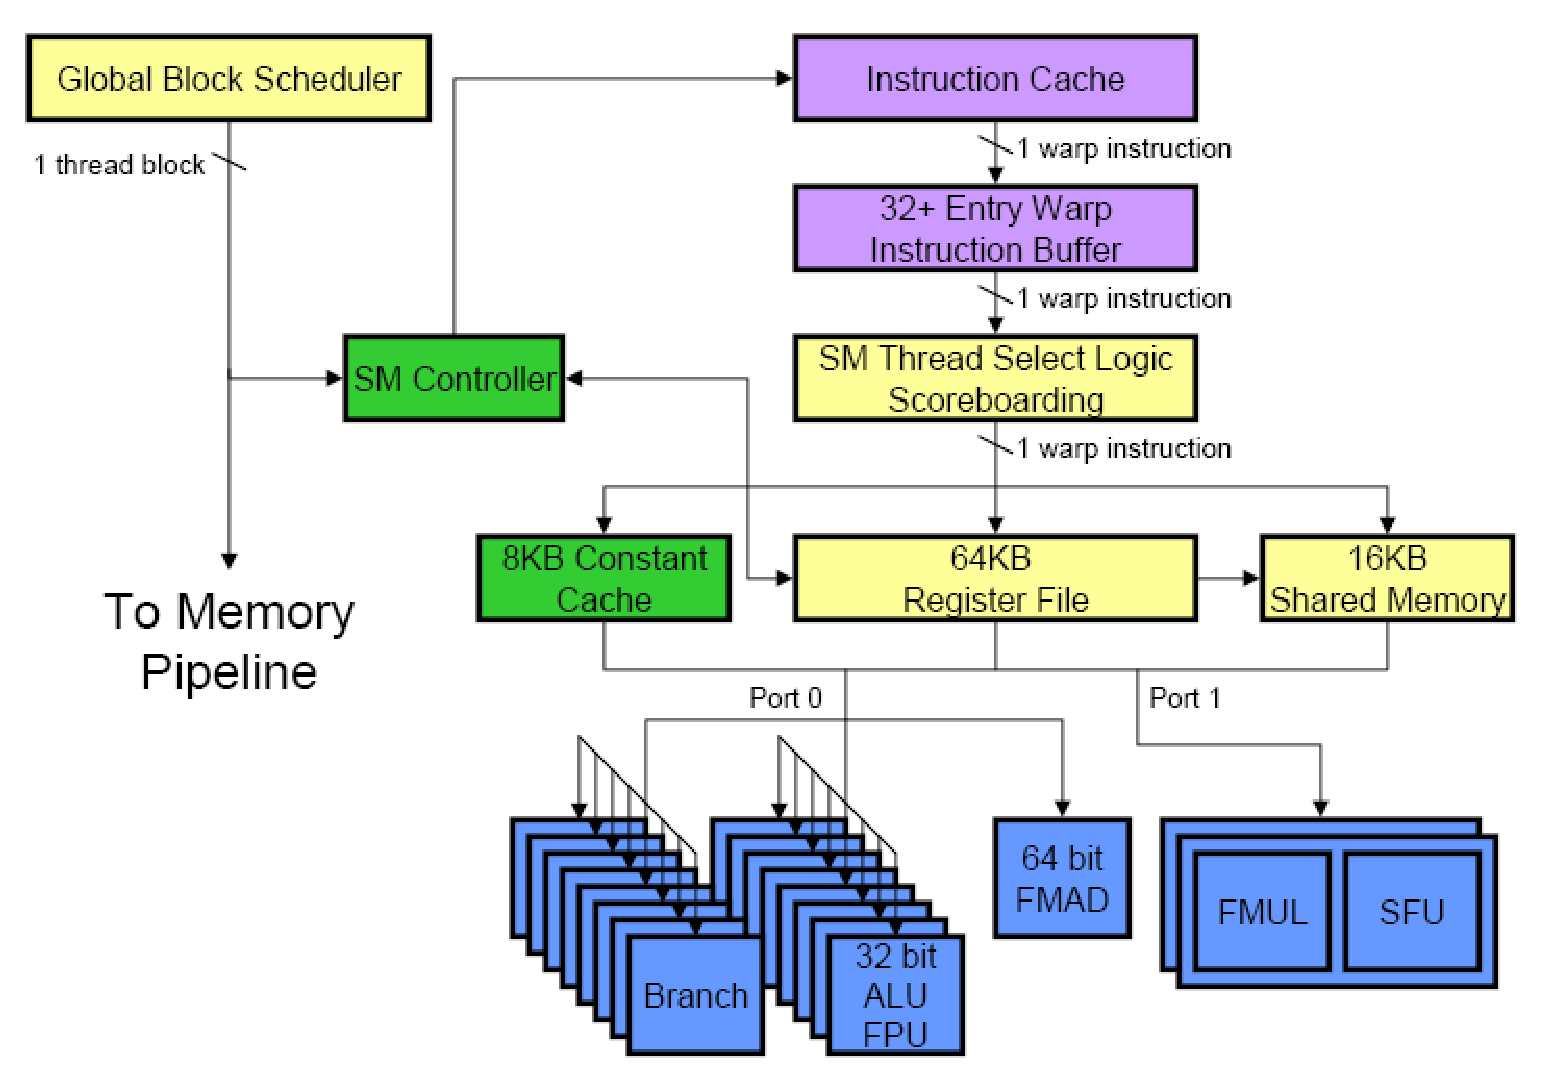
\includegraphics[height=7cm,
    angle=0]{./images/gt200_sm.eps}}
  \caption{Architecture of a GT200 streaming multiprocessor\footnote{\url{http://www.realworldtech.com/page.cfm?ArticleID=RWT090808195242&p=9}}}
  \label{fig:gt200_sm}
\end{figure}


\begin{figure}[hbt]
  \centerline{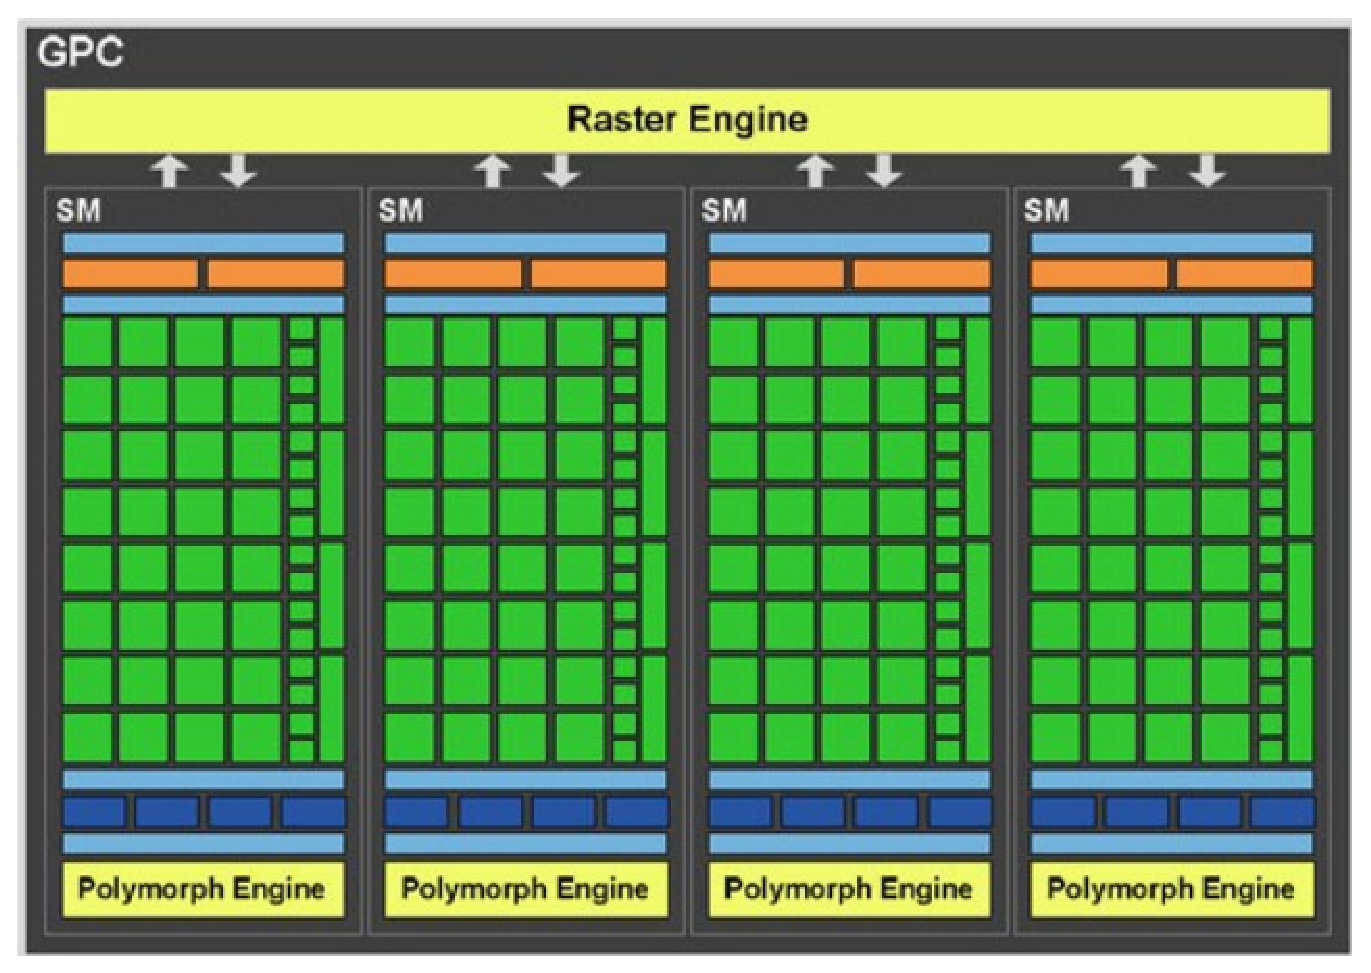
\includegraphics[height=5cm,
    angle=0]{./images/Fermi_GPC.eps}}
  \caption{A single GPC in GF100 architecture}
  \label{fig:Fermi_GPC}
\end{figure}


In Fermi, the number of double-precision CUDA cores is 7x times than
those in GT200. However, the speed-up that we can reach in many
applications is lower than that, e.g. about 4x in matrix
multiplication, Fig.~\ref{fig:matrix_mul}. The reason is that other
resources (registers, shared memory...) don't increase of that same
factor. 

\begin{figure}[hbt]
  \centerline{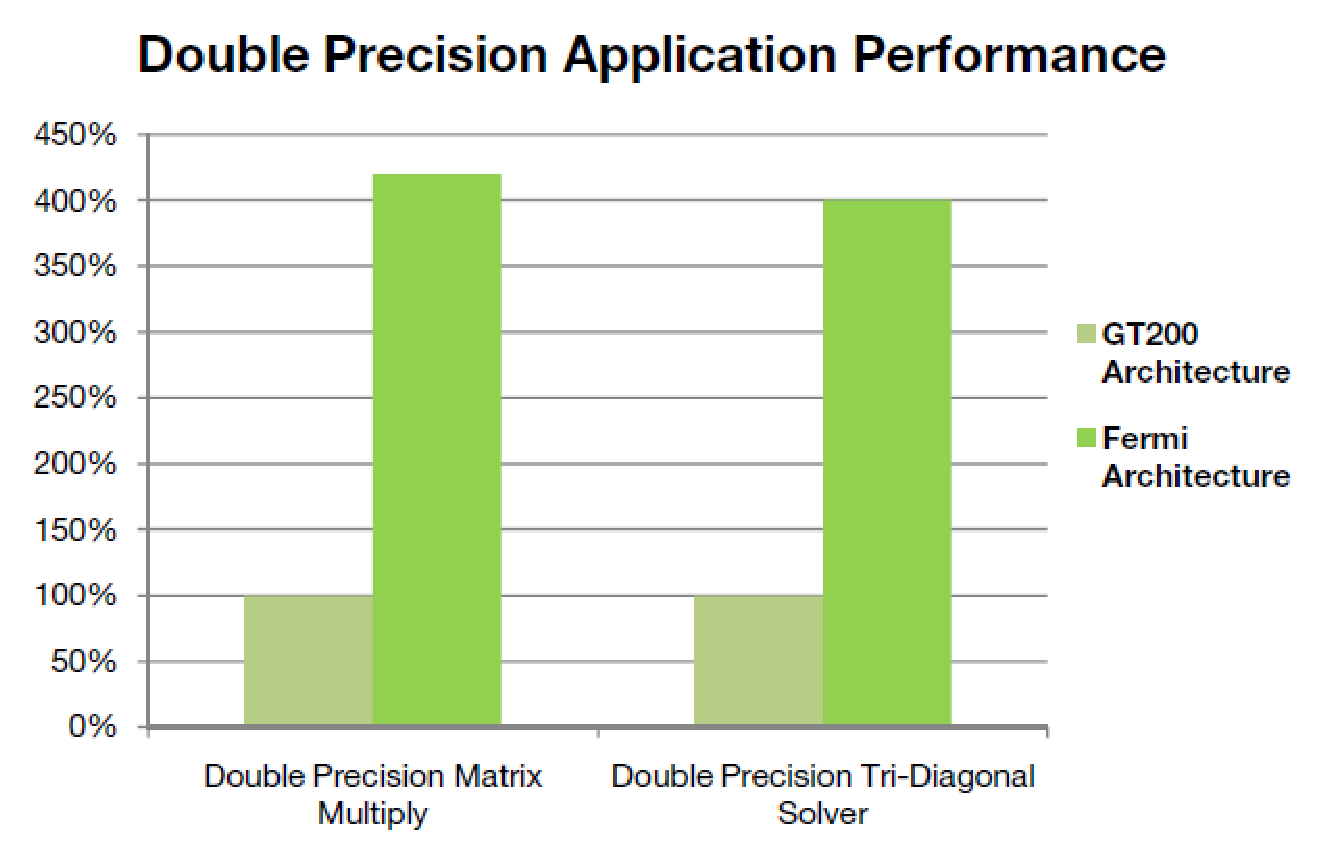
\includegraphics[height=5cm,
    angle=0]{./images/matrix_mul_fermi.eps}}
  \caption{Early performance evaluations show Fermi performing up to
    4.2x faster than GT200 in double precision applications.}
\label{fig:matrix_mul}
\end{figure}


\subsection{-- Maxwell (GM200) GPC}
\label{sec:GPC-Maxwell}

Tesla M40 (GM200) has 24 SMs or 24 TPCs

\subsection{-- Pascal (P100) GPC}
\label{sec:GPC-Pascal}

GP100 is composed of an array of Graphics Processing Clusters (GPCs), Texture
Processing Clusters (TPCs), Streaming Multiprocessors (SMs), and memory
controllers.


A full GP100 consists of six GPCs (equivalently to 60 SMs). However,
Tesla P100 accelerator uses 56 SM units or, equivalently, 28 TPCs.

With 60 SMs, GP100 has a total of 3840 single precision CUDA Cores and 240
texture units.

\begin{itemize}

  \item Each GPC inside GP100 has ten Pascal SMs (Sect.\ref{sec:SM-Pascal})
  
  \item 30 TPCs (each including two SMs).
  
  
  \item Eight 512-bit memory controllers (4096 bits total). 

  NOTE: Each memory controller is attached to 512 KB of L2 cache, 

  \item Each HBM2 DRAM stack is controlled by a pair of memory controllers. The
  full GPU includes a total of 4096 KB of L2 cache.

\end{itemize}



\section{Warp scheduler}
\label{sec:warp-scheduler}

Threads are organized into groups called warp (i.e. Nvidia uses 32 threads per
warp). All threads in the same warp execute the same instruction. When branching
occur, they are executed one by one. During the execution of one branch, only
threads satisfying the condition execute, other threads in the warp need to
wait. 

The warps are selected to use the processors by the {\bf warp scheduler}. In
Fermi, with 2 warp schedulers, two warps can be activated at once. The
instruction of threads in one warp is sent to the CUDA cores in one SM by the
instruction dispatch units. With 2 warp scheduler, it also need 2 instruction
dispatch units, each one issues one independent instruction from one warp.

Processors are selected in groups to execute the instruction. In Fermi, a group
of 16 CUDA cores are selected at once to run the instruction. The data are
loaded using the 16 LD/ST units [NOTE: Earlier Tesla selecte CUDA cores in
group of 8]. 

In most cases, two instructions from two warps can be issued at once (e.g. two
integer instructions, two floating instructions or a mix of integer, floating
point. However, double-precision instructions do not support dual dispatch with
any other instructions. So, if one warp execute a double-precision instruction,
the other warp need to wait until the double-precision is dispatched. [NOTE:
This restriction is removed in Kepler].

References:
\begin{itemize} 
  \item in Fermi: \ref{sec:warp-scheduler-fermi}
  \item 
\end{itemize}

\section{Texture (TEX) unit}
\label{sec:texture-unit}

In Tesla 1 and 2, texture units and L1 texture cache are at TPC level,
where 2 or 3 SMs shares one texture unit and one L1 texture cache. The
purpose of TEX unit is to rotate or resize bitmap to be placed on an
arbitrary 3D object as a texture. Each TEX unit computes a texture address and
fetches 4 texture samples per clock. The results can be filtered or
unfiltered. Different filter modes can be used: bilinear, trilinear and
anisotropic.



\subsection{Texture (TEX) unit}
\label{sec:texture-unit-Fermi}

TEX unit is described in Sect.\ref{sec:texture-unit}. In GF100, TEX unit and L1
texture cache have been brought to SM level. Each SM has 4 texture units.

Each unit could compute 1 texture address and fetch 4 32bit/INT8 texture samples
\textcolor{red}{per 1 clock}, 2 64bit/FP16 texture samples \textcolor{red}{per
clock}, or 1 128bit/FP32 texture sample \textcolor{red}{per clock}. 

Texture units and L1 Texture caches at SM level can run at higher clock speed
[NOTE: texture units on previous architecture run at the core clock of GPU].

With unified L2 cache, the maximum cache size for texture is 3x higher than
GT200, improving hit rates in texture heavy shaders. 

GK100 texture unit supports for
\begin{enumerate}
  \item  DirectX 11's BC6H and BC7 texture compression formats.
  \item jittered sampling, i.e. DirectX 11's four-offset Gather4 feature in
  hardware (allowing 4 texels to be fetched from a 64x64 pixel grid with a
  single texture instruction).
\end{enumerate} 

GF104 texture units improved this to 4 samples/clock for both 32bit
and 64bit, and it's these texture units that have been brought over
for GF110. GF110 can now do 64bit/FP16 filtering at full speed versus
half-speed on GF100, and this is the first of the two major steps
Nvidia took to increase GF110's performance over GF100's performance
on a clock-for-clock
basis\footnote{\url{http://www.anandtech.com/show/4008/Nvidias-geforce-gtx-580/2}},
Fig.~\ref{fig:texture_unit}.

\begin{figure}[hbt]
  \centerline{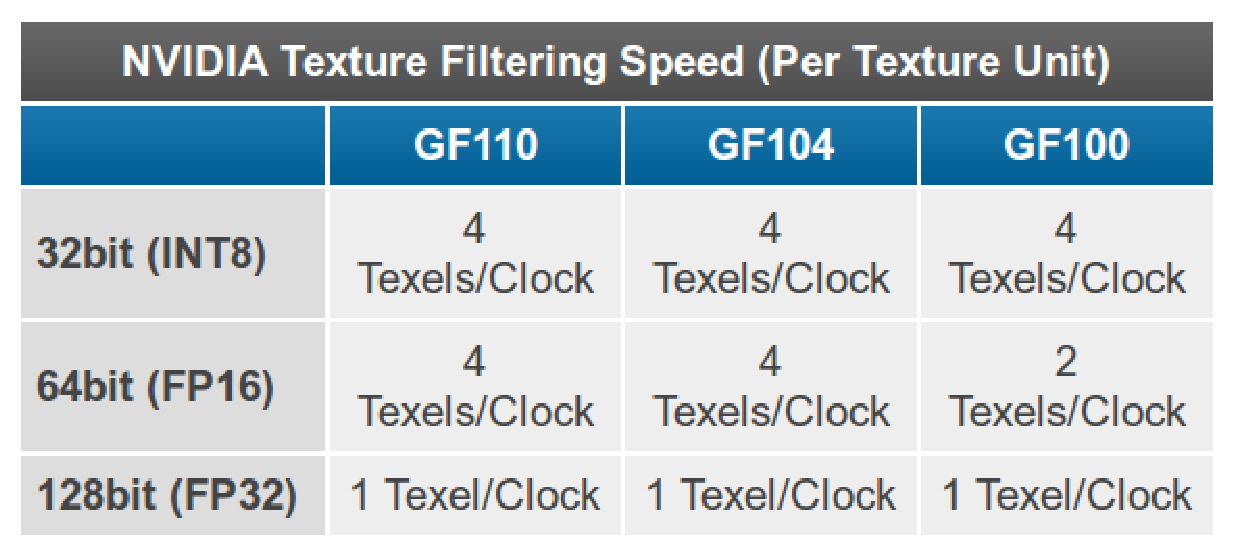
\includegraphics[height=5cm,
    angle=0]{./images/texture_unit.eps}}
  \caption{Texture units}
  \label{fig:texture_unit}
\end{figure}

\section{PolyMorph Engine}
\label{sec:PolyMorph-Engine}


\subsection{PolyMorph Engine (geometry unit)}
\label{sec:polymorph-unit-+}

PolyMorph Engine in Kepler is version 2.0. 

GT200 has only a single PolyMorph engine residing at the front-end of
the graphics pipeline. Thus, the traditional pipeline has tessellation
unit in the front of the pipeline with the (edge) setup and
rasterization units (as in AMD/ATI RV870). This can be a bottle neck
where tessellation is utilized heavily. 

Nvidia revolutionized this to enable high triangle rates under the most
demanding scenarios by incorporating a hardware {\it tessellator unit} in
PolyMorph Engine and provide each SM a PolyMorph engine.

As described in Sect.\ref{sec:Fermi_graphics-enhancement}, a newly-designed
Polymorph Engine is a new execution unit developed in Nvidia Fermi GPU card.

{\bf Each SM in Fermi has one PolyMorph Engine}. PolyMorph Engine is the execution
unit that handle geometry in 5 stages: Vertex Fetch, Tessellation, Viewport
Transform, Attribute Setup, and Stream Output. This design support DirectX11,
where Tessellation is brought from CPU to GPU
design\footnote{\url{http://www.anandtech.com/show/2918/2}}.

Each PolyMorph Engine contains a Tessellation Unit, an Vertex Fetch (Attribute
Setup) Unit, and other Geometry Processing Units. Along with this is the use of
4 Raster Engines, which allowing 4 triangles to be setup per clock. Together,
they enable breakthrough triangle fetch, tessellation, and rasterization
performance.

\textcolor{red}{The results from one stage are sent to the SM to
  process; and then sent back to the next stage. At the last stage,
  the results are sent to the Raster Engine}.
\textcolor{blue}{The Tessellator is one of the biggest change that
  DX11 brought to GPU design}
to be well used in DX11 and future
games)\footnote{\url{http://www.anandtech.com/show/2977/Nvidia-s-geforce-gtx-480-and-gtx-470-6-months-late-was-it-worth-the-wait-/3}},
Fig.~\ref{fig:polymorph}.


\begin{framed}
Tessellation is a vertex operation (tesselation adds extra geometry detail
on-the-fly for less angular objects and characters).
\end{framed}

The {\bf geometry pipeline} (geometry unit) has been significantly
revamped with improved performance in geometry shading, stream out,
and culling. Fillrate has also been improved which enables multiple
displays to be driven simultaneously by GF100 SLI, much like AMD's
Eyefinity; but now additionally in 3D and at 120 Hz.

\begin{framed}
  In Fermi, each SM has a PolyMorph engine $\rightarrow$ GF100 has 16
  PolyMorph Engines (indeed 2 of them are disable). Even though a
  single PolyMorph engine is still an in-order design, the
  availability of 16 different PolyMorph engines allows the
  Out-of-Order (OoO) execution, as GF100 need to keep track of what
  each engine is doing to maintain the integrity of the results. To do
  this, GF100 has a separate communication channel between the
  PolyMorph engines.
\end{framed}

\begin{figure}[hbt]
  \centerline{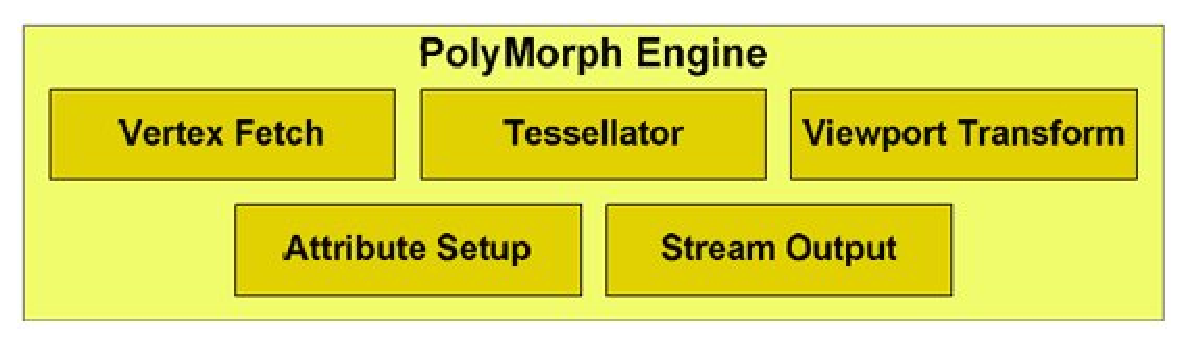
\includegraphics[height=2cm,
    angle=0]{./images/polymorph.eps}}
\caption{PolyMorph}
\label{fig:polymorph}
\end{figure}

A PolyMorph Engine handles vertex fetch, tessellation, viewport transform, 
attribute setup, and stream output
\begin{enumerate}
\item Vertex Fetch: fetching vertices from a
  {\it global vertex buffer}; then, these vertices are sent to the SM
  for vertex shading and hull shading. In these two stages the
  vertices are transformed from object space to world space, and
  calculate tessellation factors.

\item Tessellator: receive the tessellation factors and then dices the
  patch and outputs a mesh of vertices. The new vertices are sent to
  the SM where the Domain Shader and Geometry Shader are executed.

  The Domain Shader calculates the position of each vertex based upon
  input from the Hull Shader and the Tessellator. At this stage a
  displacement map is usually applied to add detailed features to the
  patch. The Geometry Shader conducts post processing adding and
  removing vertices and primitives where needed. The final results are
  sent to the Tessellator for the final pass.

\item ViewPort Transform: receive the result from SM, it performs viewport
  transformation and perspective correction. 

\item Attribute setup follows, transforming post-viewport vertex
  attributes into plane equations for efficient Shader evaluation.

\item Finally, vertices are optionally
  "streamed out" to memory making them available for additional
  processing\footnote{\url{http://www.motherboards.org/reviews/hardware/2038_4.html}}. 
\end{enumerate}

\begin{framed}
  
  The newly generated primitive shapes are converted to pixels using
  Raster Engines. GT200 has a single Raster Engine. In Fermi, every 4
  SMs has a Raster Engine. So, a group of 4 SMs in Fermi now can
  function as an individual GPU chip. Thus it is given the name
  Graphics Processing Cluster (GPC).  ATI RV870 has two raster
  engines.
\end{framed}


The total PolyMorph Engine in GTX 680 (Kepler) is 8, which is half of that in
GTX 580 (Fermi). However, the performance is roughly double per-clock of the
Fermi version. With 30\% higher in clock speed, it means the overal performance
of PolyMorph Engine in Kepler GTX 680 is higher than that in Fermi GTX 580, i.e.
a polygon is spurred in about 2 cycles in GK104 instead of 4 in GF100
\footnote{\url{http://www.tomshardware.com/reviews/geforce-gtx-680-review-benchmark,3161-2.html}}.

\section{Raster Engine}


\subsection{Raster Engine}
\label{sec:raster_engine}

The Raster Engine does basic setup elements to the primitives given to it after
being processed by PolyMorph Engines (Sect.\ref{sec:polymorph-unit-+}).
In particular, newly generated primitives are converted to pixels using the
Raster Engines before sending to the Display Monitor. To achieve high triangle
throughput, GF100 use 4 Raster Engines.
\begin{enumerate}
\item Edge (triangle) setup: vertex positions from the PolyMorph
  Engine are fetched and triangle edge equations are
  computed. Triangles not visible on the screen are removed via back
  face culling. Each edge setup unit processes up to one line, point
  or triangle per clock. 

  With 4 Raster Engines,
  \textcolor{red}{ GF100 can do 4 triangle setups per clock maximum}.

\item Rasterization: rasterizer takes the edge equations for each
  primitive and computes pixel coverage. If anti-aliasing is enabled,
  coverage is performed for each multisampling and coverage sample.
  \textcolor{red}{Each Rasterizer outputs eight pixels per clock for a
    total of 32 rasterized pixels per clock across the chip}.

\item Z-cull: Raster Engine performs Z-Cull which allows hidden
  surfaces not to be rendered saving bandwidth.
\end{enumerate}

\textcolor{red}{Raster Engine}: Each GPC has a {\bf Raster Engine}. It is
composed of 3 pipeline stages: triangle setup (edge setup), rasterization and
Z-cull, Fig.~\ref{fig:raster_engine}.

\begin{figure}[hbt]
  \centerline{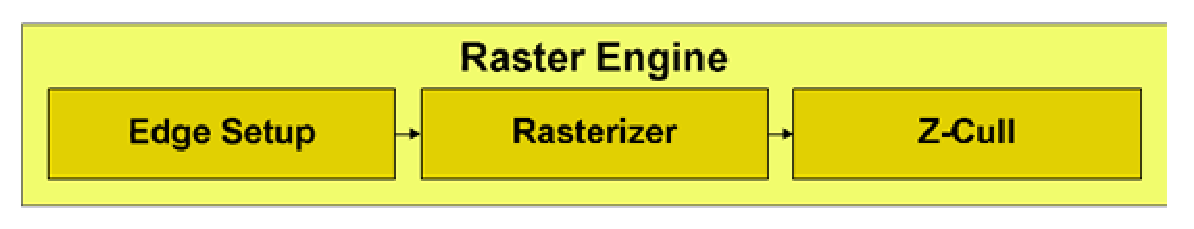
\includegraphics[height=2cm,
    angle=0]{./images/raster_engine.eps}}
\caption{Raster Engine}
\label{fig:raster_engine}
\end{figure}



\begin{framed}
  Rasterization-based techniques are mostly used in GPU to render
  graphics. The technique to provide better output is {\bf ray tracing},
  yet require much more intensively computation. Nvidia provide OptiX, a
  real-time ray tracing API on its GPU. Another project is
  OpenRT. Nvidia believe that ray tracing is the future of computer
  graphics.
\end{framed}

\section{Clock cycles and speeds}
\label{sec:clock-cycles-speeds}

The bell ring at school to tell the end of each class (say every 45 minutes), it
allows students to move from one class to another. A school is analogy to a CPU;
and a bell is in analogy to a clock pulse in a computer. Without the bell, some
class would be released early and some late. Similarly, a computer has multiple
components, each does a different work, and can be at different speed.
Periodically, a component send data along the wire to the next processing
station. To coordinate the activity, the computer uses a {\it clock pulse},
which is the crystal oscillator. Crystal oscillator is an electronic device that
create an electrical signal with a very precise frequency, typically, of
producing fixed since wave, which is then sampled to convert to hig and low
voltage.\footnote{\url{http://www.yale.edu/pclt/PCHW/clockidea.htm}}

With alternating high ('tick') and low ('tock') voltage, each tick-tock is a
{\bf cycle}, and the length (i.e. the delay from tick to tock) is often in
nanoseconds (\textcolor{red}{One nanosecond is the time for an electrical signal
to travel about one foot}), and then mapped to frequency (in Hz, MHz).
The standard external {\it clock speed} is a multiple of 33.3333...
MHz. By convention, the speed is round down to 33 MHz or 66 MHz. The other
values: 100 MHz (3x of 33.3333\ldots MHz), 133 MHz, 166 MHz or 200 MHz.
\begin{Verbatim}
    Clock   Cycle    Bus
        33Mh    30 nsec    PCI (general adapter cards)
        66Mh    15 nsec    AGP (video adapter)
        100Mh   10 nsec    mainboard clock to the CPU
        2Ghz     0.5 nsec  CPU internal clock after multipler
\end{Verbatim}
One GHz refers to one billion of times per minute the CPU's clock pulses into
the microprocessor. The clock pulse tells some circuits when to start sending data
on the wires, while it tell other circuits when the data have arived. NOTE:
\textcolor{red}{Data can be transferred at a higher frequency than the clock
rate}. With early CPUs, each has a single clock whose signal applies to CPU,
memory and all I/O devices. Modern CPUs has different clocks with different rates.
Generally, all clocks have the rate as a multiple of a given standard clock
speed as given above. An example is 
\begin{enumerate}
  \item CPU socket clock: signal generated by the mainboard to pace data
  transfer to/from CPU with memory/AGP video card/IO device. This is known as
  the standard {\it external clock speed}. The mainboard sense the CPU model
  and use the default speed
  
  The motherboard socket is the location into which the CPU processor will sit,
  which evolves over time. Two types of sockets from AMD are FM1 (using for APU
  - Chap.\ref{chap:unifying-cpu-gpu}) and AM3+ (using Bulldozer-based CPU
  and backward compatible with older CPUs). Two types of sockets from Intel are
  LGA115 and LGA2011. Older sockets from Intel are LGA1166, LGA1366.

\begin{verbatim}
Chip Type  Actual Clock  Bits/Clock  FSB  Multiplier  Speed

Pentium 4 2.4  100 MHz  4  400 MHz  24  2.4 GHz
Pentium 4 2.4A  133 MHz  4  533 MHz  18  2.4 GHz
Athlon XP 2400  133 MHz  2  266 MHz  15  2.0 GHz
\end{verbatim}  

  
  \item FSB clock: The CPU sends data, in bits, to the Northbridge chip on the
  mainboard (before going to the memory/AGP-card/IO-device) at a faster rate
  than the CPU socket clock, Fig.\ref{fig:mainboard_diagram}. 
  Thus, the CPU clock speed is
\begin{verbatim}
FSB clock speed = (actual-clock) x (transfer-rate)
\end{verbatim}
Newer CPU doesn't use FSB as there is no Northbridge between CPU and other
devices, e.g.
Athlon 64 CPU chip has its own integrated memory controller inside the CPU and a
high speed HyperTransport integrated I/O bus. 
Thus FSB clock speed would be meaningless.

\begin{mdframed}
Front Side Bus (FSB) is the external bus, shared between memory and I/O request.
With the newer generation of Intel CPU, an embeded memory controller is added,
called IMC (Integrated Memory Controller). These CPUs comes with QPI technology
(Quick Path Interconnect) (Sect.\ref{sec:QPI_IOH}). 
\end{mdframed}
  
  \item CPU clock speed: the {\it internal clock} of the CPU run at a faster
  speed than the socket clock speed, via a {\bf multiplier}
  
  \item Memory clock: the modern motherboard can generate a separate clock to
  the memory (example clock rate 100, 133, 166, and 200 MHz). DDR RAM can
  generate twice the actual clock speed (200, 266, 333, or 400 MHz).
\end{enumerate}
Due to the different clock speed, the overall performance is determined by the
slowest one. Example: The FSB run at 800 MHz, and the memory runs at 400 MHz. To
avoid this problem. The newer mainboard requires the DDR RAM should be installed
in pairs and using two separate memory busses. The memory reference is split
between the two 400 MHz buses, and producing an aggregate transfer rate 800 MHz.
\footnote{\url{http://www.yale.edu/pclt/PCHW/clockidea.htm}}

\begin{figure}[hbt]
  \centerline{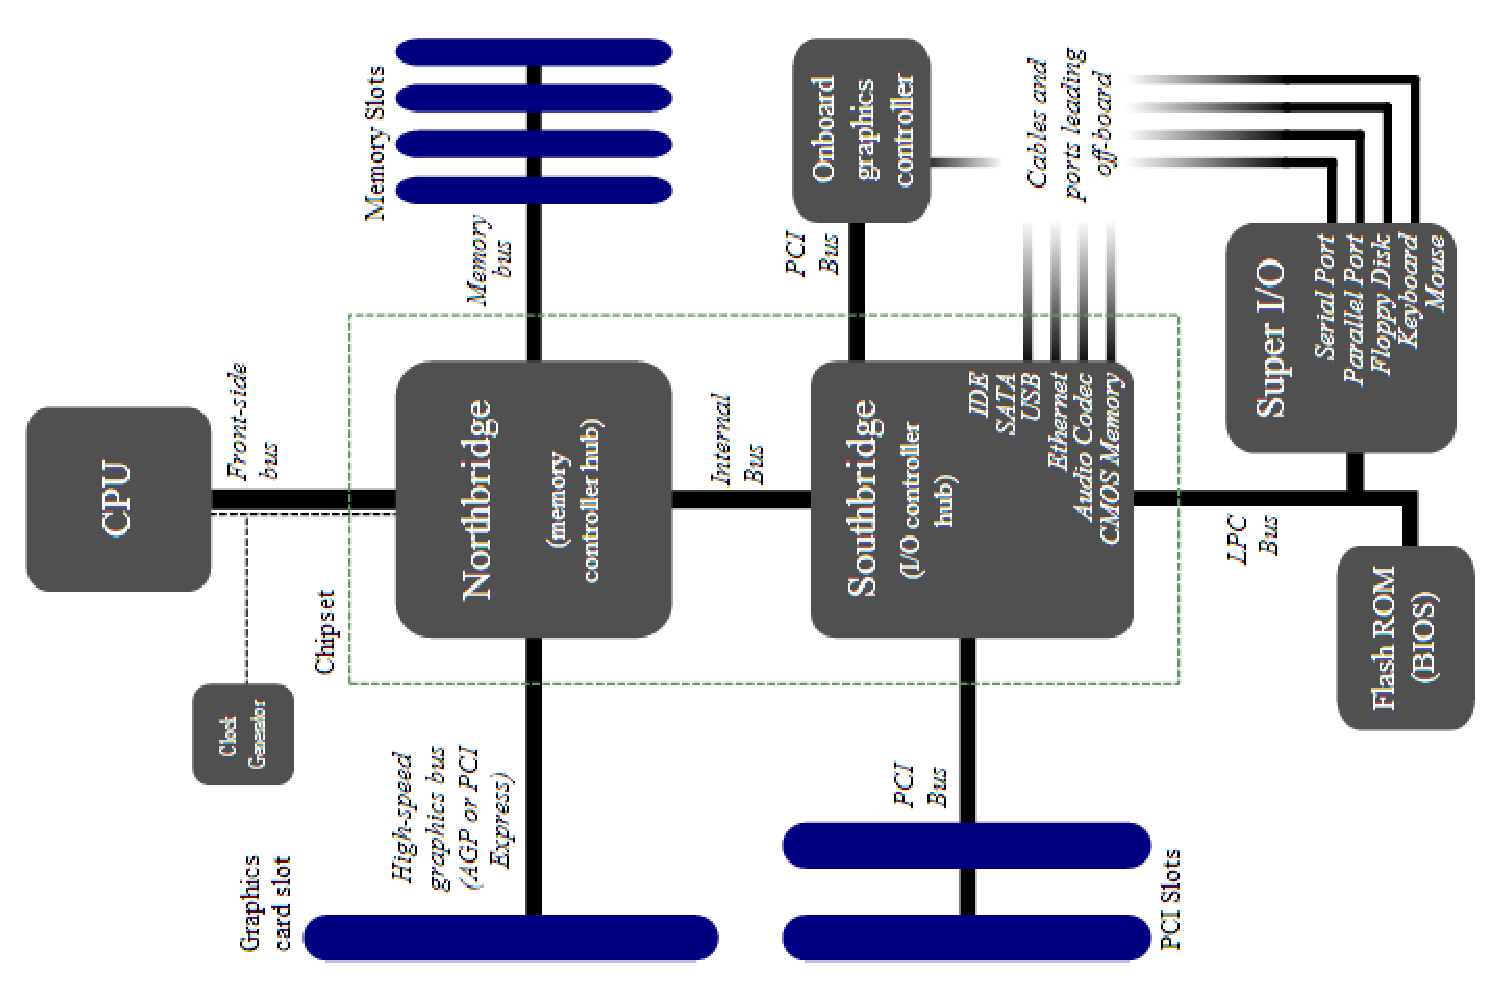
\includegraphics[height=5cm,
    angle=0]{./images/mainboard_diagram.eps}}
\caption{Connectivity between different components on a mainboard}
\label{fig:mainboard_diagram}
\end{figure}


\textcolor{red}{There are two clocks: the internal CPU clock rate and external
clock rate}.
The clock multiplier (CPU multiplier, CPU core ratio) is the speed ratio of the
internal CPU clock rate vs. the external clock rate. This is typically fixed
during manufacturing. Some motherboards has the option to change using BIOS
setup (OverClock section, e.g. CPU core (Non-Turbo) ratio) which makes the CPU
run faster (TUAN)
\begin{itemize}
  \item Intel 2.4 Pentium 4: with a 100 MHz
internal clock speed, data is transferred at 4x per clock tick, then the I/O
(front-side-bus FSB to memory) is 400 MHz. The CPU has a 'multiplier' of 24,
the internal clock rate is 24x100 = 2.4 GHz.

  \item Intel 2.4A Pentium 3: with 133 MHz internal clock speed, the Front-Side
  Bus is 533 MHz. Using the multiplier of 18, then the internal clock rate is
  18x133 = 2.4 GHz.
\end{itemize}
Newer Intel and AMD CPUs use a new technology that doesn't limit the clock speed
to standard values (Intel Turbo Boost, AMD Turbo Core). This enables the
processor to run at a higher speed automatically, i.e. no need to adjust BIOS
setting, for a short period of time. Example: a 3.3GHz Core i7-3960X Extreme
Edition can run at 3.9 GHz.

\begin{mdframed}
To improve the CPU
\begin{enumerate}
  \item faster clock speed: reduce the time for each class and student need to
  learn faster
  
  \item build a pipeline: instead of using 45-min class, break down into 15-min
  class, as some 45-min class doesn't use all 45-min.
  
  \item parallelism: add more classrom. Only works if the school has more
  students, i.e. the CPU has more data
  
  \item class size: double the number of students in each class room (only if
  there are more students studying the same course), e.g.  from 32-bit to 64-bit
  data-oriented operation 

  
  \item build another school: use multi-core architecture
   
\end{enumerate}
The first option is the easiest; however it soon reaches the limit. In 2004,
Intel reached the almost limit, 3 GHz. AMD even though has lower clock rate 2
GHz, it has more parallelism (first switching to 64-bit), and thus is still as
much powerful as Intel chip.  Then, multi-core is added
(Sect.\ref{sec:core-thread}). 

\end{mdframed}

The GPU chip is a processor just like a CPU on the mainboard. The videocard,
e.g. GTX560 is where the GPU chip reside. So GTX 560 is not a GPU, it's a
videocard. The details is given in Fig.\ref{fig:GPU_videocard}.


\begin{figure}[hbt]
  \centerline{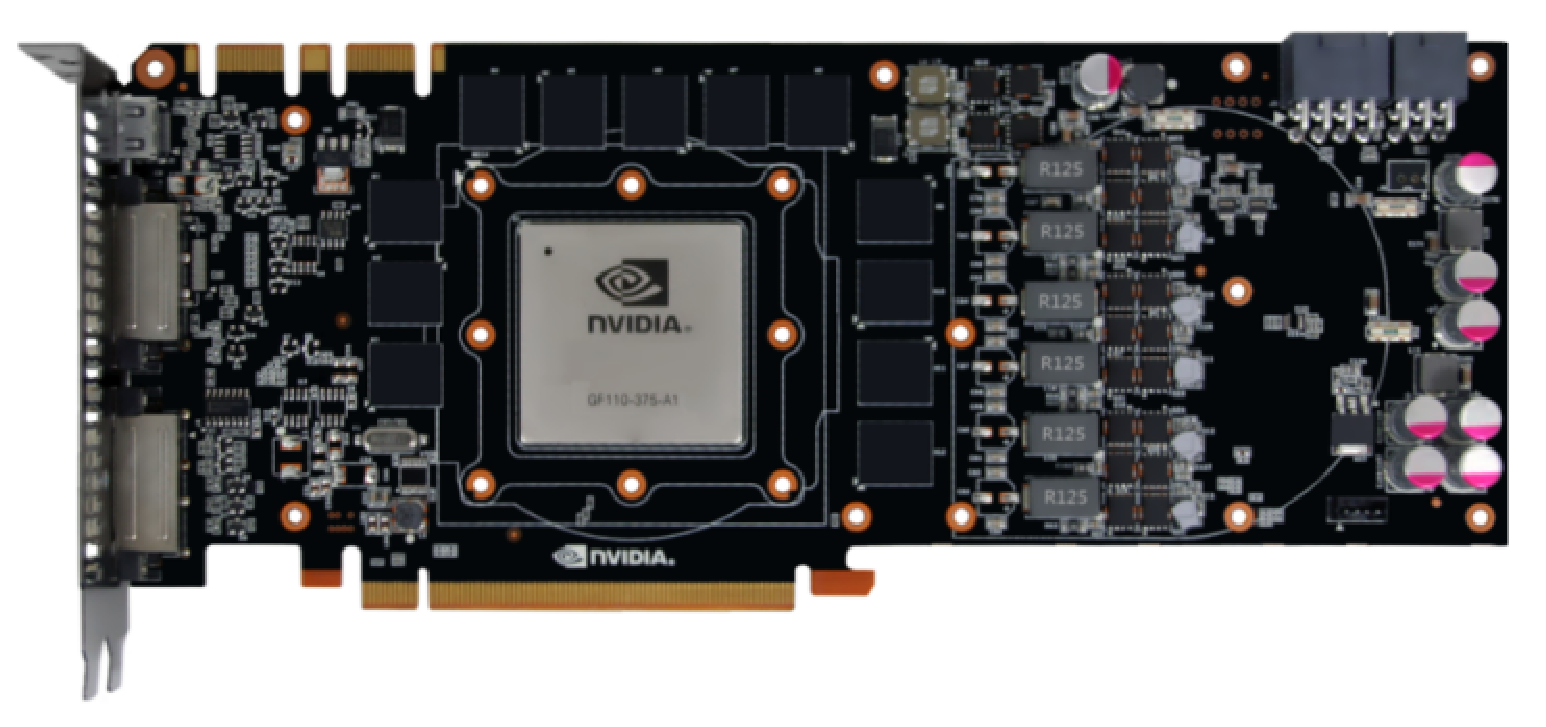
\includegraphics[height=8cm,
    angle=0]{./images/GPU_videocard.eps}}
\caption{GTX580 videocard: The large NVIDIA chip is the GPU chip (here is
GH110). The 12 smaller ships surrounding it is the video RAM chips (which is
GDDR5 in this case). The bus connection between one RAM chip with the
GPU chip is 64-bit. , i.e. total 64x6=384 bits}
\label{fig:GPU_videocard}
\end{figure}


On Nvidia GPU, there are 3 ``clocks'', corresponding to speed of core clock,
shader clock (graphics clock), and memory access (memory clock). 
\begin{itemize}
  \item {\bf Memory clock}: How many times a memory access per second.
  %The speed of the GPU defined in terms of this

\item With unified architecture, each GPU core can handle any tasks. However,
depending on the task it does (i.e. general purpose computation or graphical
processing), the GPU core can run at different clocks. If  it does shading, the
clock is {\it shader clock} (or graphics clock). If it does general-computing,
the clock is {\it core clock}.

ATI set the speed of {\bf core clocks} and {\bf shader clocks}  the same.
However, Nvidia set them different (core clock (processor clock) is 2x shader
clock), until Kepler architecture (Chap.\ref{chap:Kepler}). Nevertheless, it
doesn't mean core and shaders are different, it just the GPU cores run at
different speeds when doing different things.
\end{itemize}

\begin{verbatim}
# of ROPs x Core Clock = Pixel Fill Rate
\end{verbatim}
Example: GTX 470: 40 x 607.5 MHz = 24.30 GPixel/s. So GTX 475 with 32 raster
operators to have the same performance, it needs a higher clock, e.g. 32 x 760
MHz = 24.32 GPixel/s.


\begin{framed}
\textcolor{red}{The core clock runs some functions on the 
multiprocessor level},  like the instruction decoder or control logic or storage
arrays, and  \textcolor{red}{the shader clock runs the individual processors}. The
shader clock is thus the fastest of the two, and this sets the speed
of arithmetic operations by the processor. Shader clock is 2.5x the
core clock (see Clock rate on Hardware specification).
The term ``hot clock'' refers to the fastest clock - the shader clock. Shader
clock was introduced in G80 Tesla-architecture GPU and was used in Tesla- and
Fermi-architecture GPUs.
\end{framed}

\textcolor{blue}{Since GF100, {\bf core clock} concept is no longer present} as
everythings tights to the shader clock (graphics clock). Only the ROPs and L2
cache operate on a separate clock domain. Everything else runs at a derivative
of the shader clock. The execution hardware runs at the full shader clock speed,
while the texture units, PolyMorph and Raster Engines all run at 1/2 shader
clock speed.

\section{Error Correcting Code (ECC)}
\label{sec:ECC}


\textcolor{red}{ECC in GDDR5}:
GK110 Kepler GPUs offered ECC protection for GDDR5 by allocating some of the
available memory for explicit ECC storage. 6.25\% of the overall GDDR5 is
reserved for ECC bits.
The register files, shared memories, L1 cache, L2 cache, and the GDDR5 are
protected by a Single‐Error Correct Double‐Error Detect (SECDED) ECC code.


In the case of a 12 GB Tesla K40 (for example), 750 MB of its total memory was
reserved for ECC operation, resulting in 11.25 GB (out of 12 GB) of available
memory with ECC turned on for Tesla K40.

Also, accessing ECC bits caused a decrease in memory bandwidth of 12-15\% on
typical workloads, compared to the non-ECC case.

\textcolor{red}{ECC in HBM2}:
Since HBM2 supports ECC natively, Tesla P100 does not suffer from the capacity
overhead, and ECC can be active at all times without a bandwidth penalty.





\section{Memory architecture}
\label{sec:close-view-at}

\subsubsection{G80/G92}
\label{sec:g80g92_memory}

Let's briefly review G80/G92
architecture\footnote{\url{http://alasir.com/articles/Nvidia_fermi_architecture/}}:
it has 8 clusters (TPCs), each with 2 subclusters (SMs). Each SM has 8
pipelines SIMD (SPs).  In terms of memory, each SM has
\begin{itemize}
\item register unit with a {\it 8K 32-bit register files}
\item {\it 16KB user-managed shared memory per subcluster} shared
  equally to all SPs,
  \textcolor{red}{each SP has 2KB of shared memory to use}.
\end{itemize}
There are 2 types of read-only cache memory: cache constant (64KB
total, i.e. 8KB per cluster), L1 texture cache (128KB total, i.e. 16KB
per cluster).

With six 64-bit memory controllers (channels), G80 has 384-bit
bandwidth. Each channel (or raster partition) has 4 ROPs, i.e. 24 ROPs
in total. G92 has only four 64-bit memory channels, i.e. 256-bit
bandwidth.

\begin{itemize}
\item G90/G92 use a companion chip called NVIO to provide output
  interfaces (two RAMDACs, two DVI/HDMI transmitters, one legacy
  TV-out)
\item G80 use PCI Express v1.0, while G92 use PCI Express v2.0
\end{itemize}

\subsubsection{GT200}
\label{sec:gt200}

Let's briefly review GT200
architecture\footnote{\url{http://alasir.com/articles/Nvidia_fermi_architecture/gt200_gt300_architecture.shtml}}:
it has 10 clusters (TPCs), each with 3 subclusters (SMs). Each SM has
8 pipelines SIMD (SPs).  In terms of memory, each SM has
\begin{itemize}
\item register unit with a {\it 16K 32-bit register files}

\item {\it 24KB shared memory per subcluster} shared equally to all
  SPs, i.e.  \textcolor{red}{each SP has 3KB of shared memory to use}.
\end{itemize}
There are 2 types of read-only cache memory: cache constant (64KB
total, i.e. 8KB per cluster), L1 texture cache (128KB total, i.e. 16KB
per cluster).  GT200 has eight 64-bit memory channels, i.e. 512-bit
bandwidth. Each channel work with 4 ROPs, i.e. 32 ROPs in total.

\begin{figure}[hbt]
  \centerline{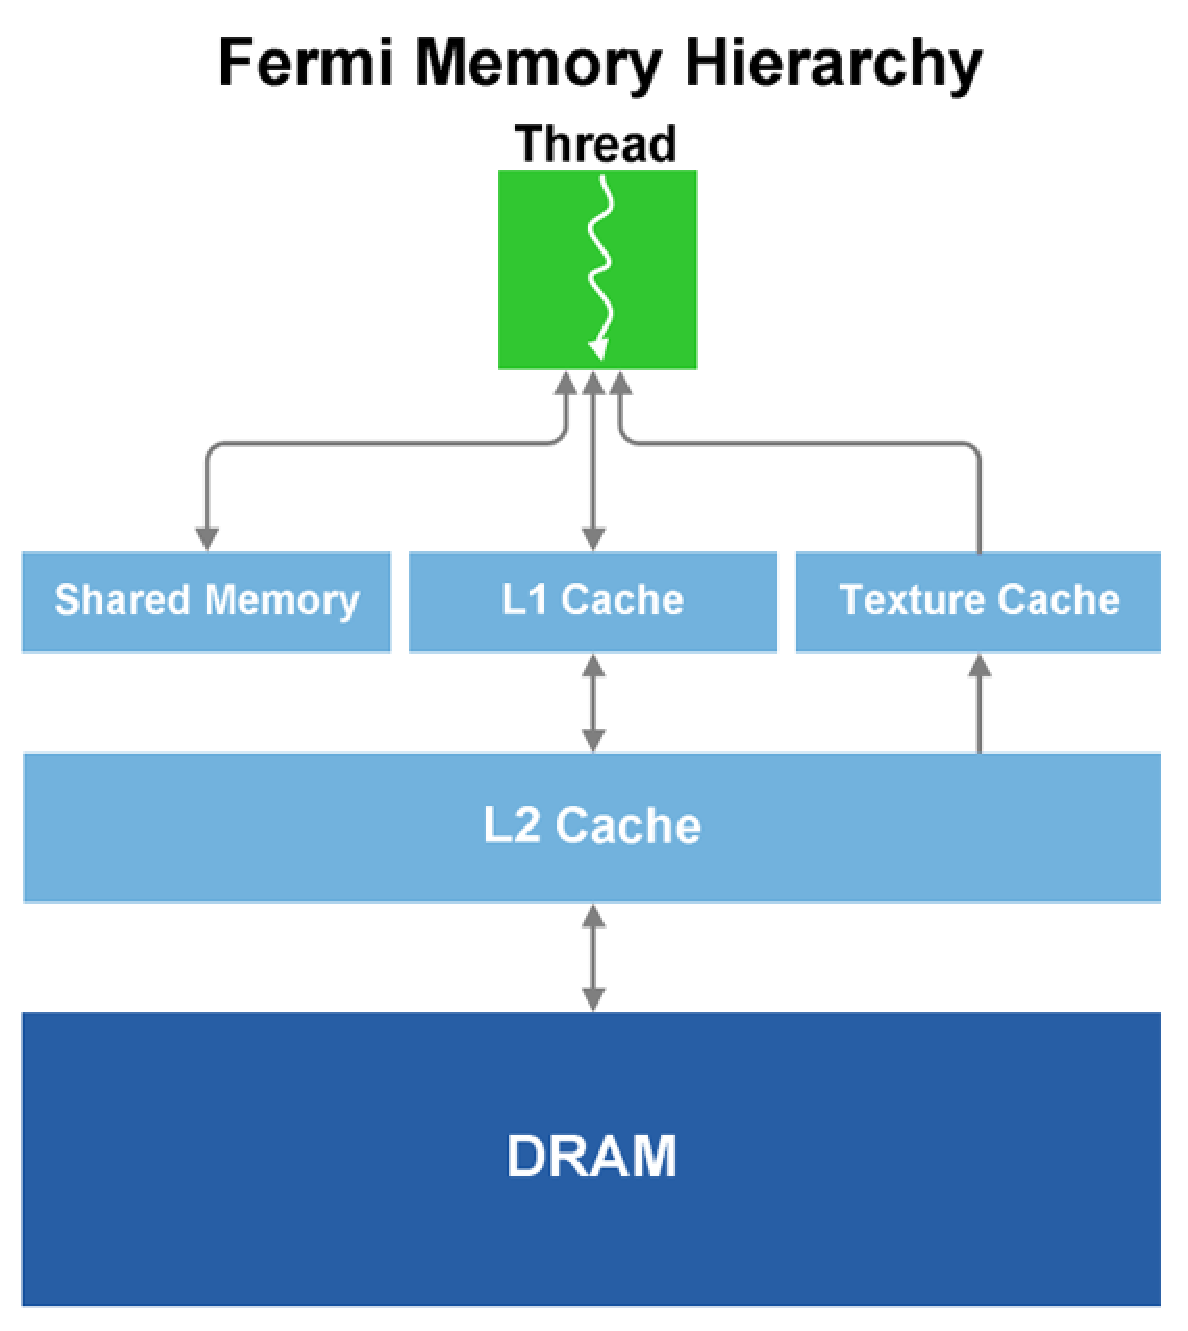
\includegraphics[height=5cm,
    angle=0]{./images/fermi_memory1.eps}}
  \caption{Fermi memory hierarchy}
  \label{fig:fermi_memory}
\end{figure}

\subsubsection{Fermi (GF100)}
\label{sec:fermi-gf100}

In Fermi, each subcluster has a local (fast) 64KB memory configurable
into shared memory ({\it software managed}) vs. L1-cache
({\it hardware managed}) in either 48KB shared memory and 16KB L1
cache, or 16KB shared memory and 48KB L1
cache\footnote{some applications have threads access the off-chip data
  more often than sharing the result data, i.e. it can increase
  performance if the data is cached; such applications need more cache
  than shared memory. Thus the configurable memory balances between
  the two application purposes},
as shown in Fig.~\ref{fig:fermi_memory}.

\begin{framed}
  Nvidia says that 64-bit instructions use all the register access
  resources, which means the dual-issue mode not compatible with double
  precision. We don't however know if, in terms of implementation, a
  single SIMD handles all operations on doubles or if 2 SIMDs run
  together at half speed, as Nvidia wouldn't give any specifics on
  this\footnote{\url{http://www.behardware.com/articles/772-6/Nvidia-fermi-the-gpu-computing-revolution.html}}.
\end{framed}

GF100 have the L2-cache memory of 768KB, i.e.  128KB of such cache per
memory controller.  This L2 cache is shared by all SM to serve all
memory controller load/store/texture requests, i.e. 48KB per SM. It
also help by caching temporary register spills of complex
programs\footnote{when the data in thread is large and the limit of
  registers, the registers for a thread may not hold all; thus
  prior-Fermi GPU need to spill them to DRAM which greatly decrease
  the performance. Now, with Fermi, it can be avoided by caching to L2
  cache. In addition, L1 cache can be used as temporary register
  usage.}
Thus, any L2 write from any cluster are visible in the next clock to
any other cluster in the chip.
\textcolor{red}{Data in L2 cache are alive between kernel calls; but
  not guarantee with L1 and not with register files.}

\begin{framed}
  In Tesla 2nd gen, shared memory is used to share data between
  threads in the same thread-block (mainly in parallel algorithms);
  data between thread-blocks need to share via the device global
  memory. Since Fermi, data in L2 cache is an alternative for sharing
  data between thread-blocks.
\end{framed}

In Fermi, register files and shared memory do not run on the fast
clock, but on the core clock. So between the register file and the
shared memory, there must be a total of 80 inputs and 32 outputs
available - an aggregate of 112 ports across all the storage array. Of
course, a couple of other units use the register files as well -
prominently the texturing unit and load store pipelines, so the total
is probably closer to 128.


\subsection{G80/G92}
\label{sec:g80g92-architecture}

A pixel is a vector of 4 components (RGBA - red,green,blue,alpha) or
also named as XYZW since they doesn't necessarily represent color
information. These 4 components are processed in parallel.

At each clock cycle, a single instruction is issued to operate on 4 pixels.
However, it often happens that an instruction isn't applied to all components,
i.e. each component use a different operation. Thus, to avoid wasting resources,
AMD/ATI shaders cores are capable of simultaneously processing 2 instructions.
\begin{verbatim}
MUL R1.xy
ADD R1.z
\end{verbatim}
This is know as ``co-issued'' or multiple-instructions multiple-data
(MIMD). However, in Nvidia, the cores are SIMD. The major difference
is that instead of processing 4 pixels of 4 components per cycle, the
scalar processor processes 1 component of 16 pixels. In G80 chips -
Nvidia's first unified architecture, the first generation of unified
shader only supports one component at a time, i.e. scalar, and thus
given the name {\bf scalar processors} (SP), and later named {\bf streaming 
processor} (SP).

\begin{figure}[hbt]
  \centerline{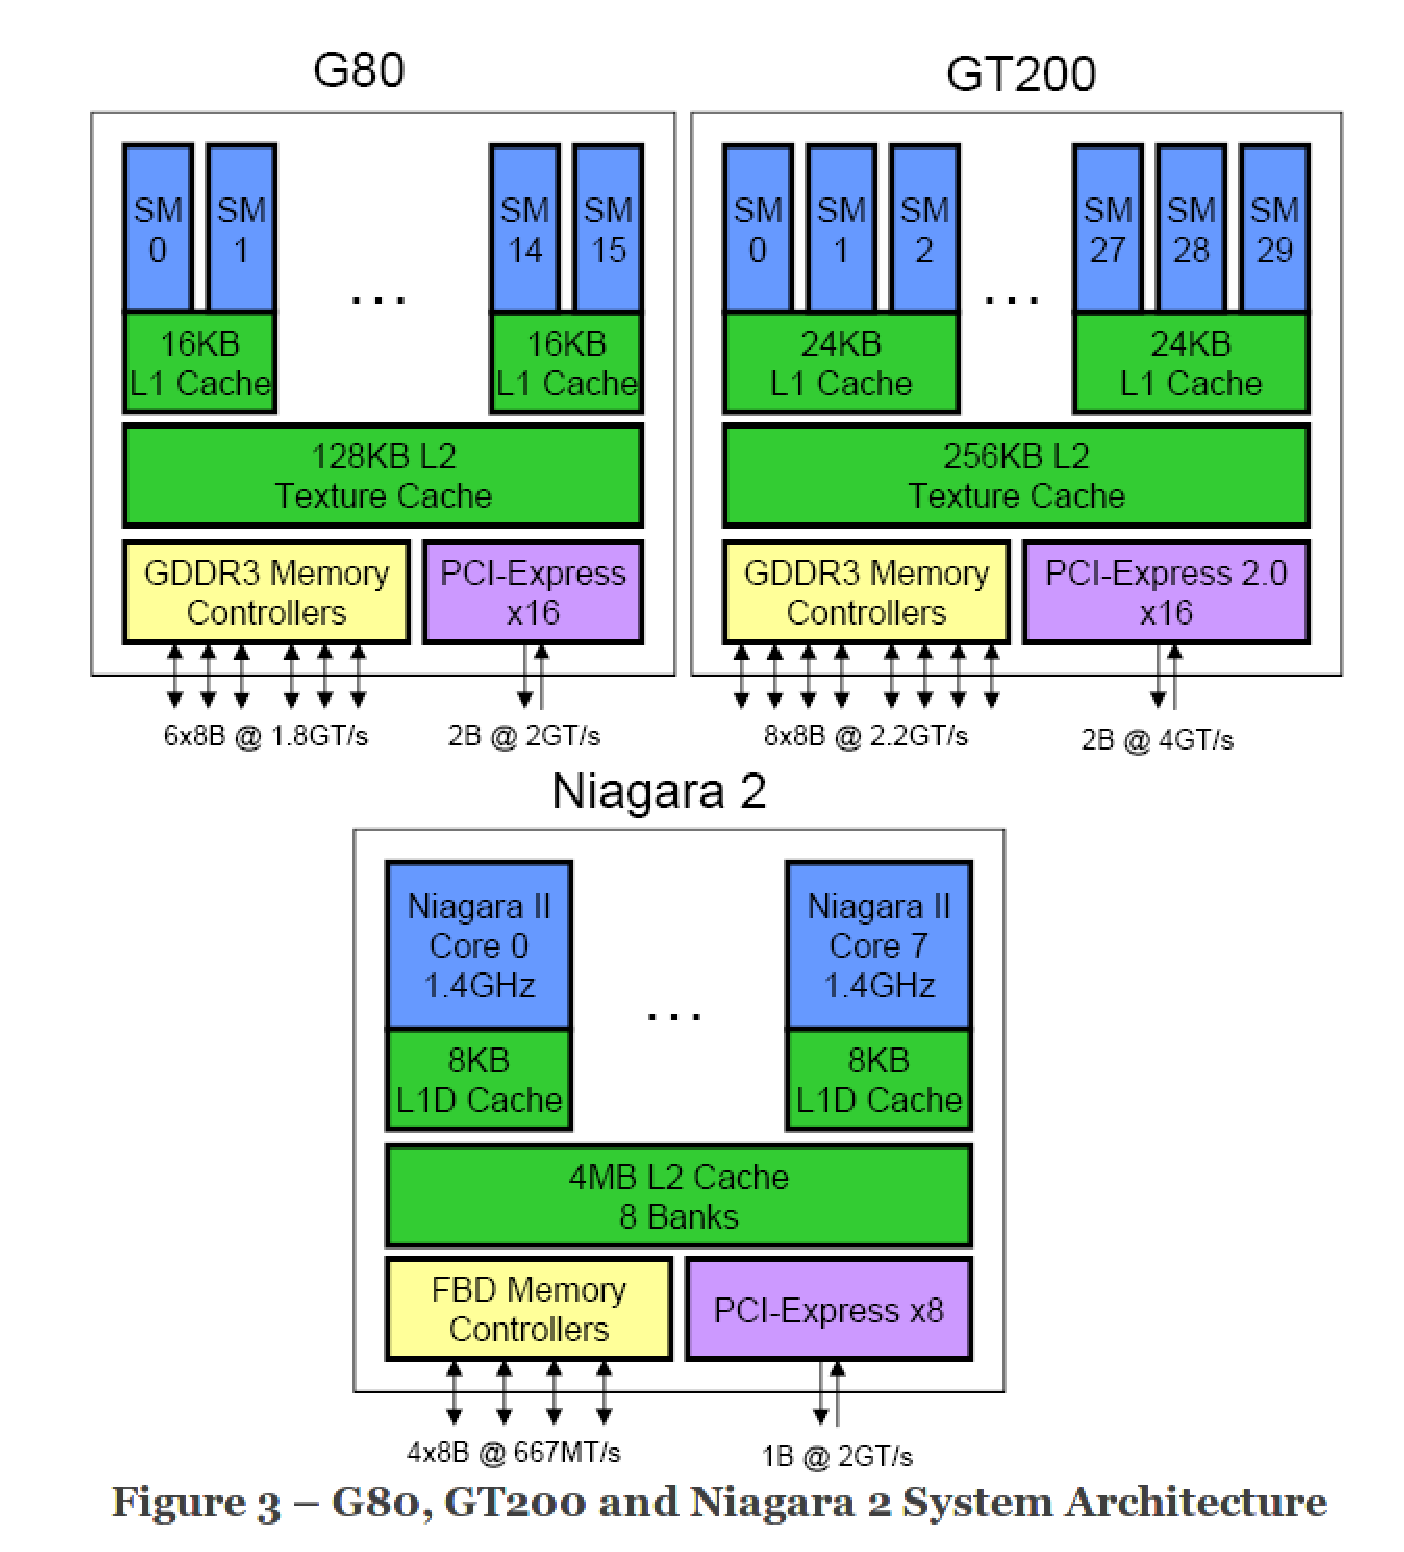
\includegraphics[height=10cm,
    angle=0]{./images/g80_gt200_niagra.eps}}
\caption{G80, GT200 and Sun Niagra 2}
\label{fig:g80_gt200_niagra}
\end{figure}



\begin{itemize}
\item GeForce 7: one instruction for a single component of 16 pixels
  take \textcolor{red}{4 clock cycles}
\item GeForce 8: one instruction for a single component of 16 pixels
  take \textcolor{red}{3 clock cycles}. A 25\% improvement due to the
  reorganization of MUL R1.xy into 2 separate MUL R1.x and MUL R1.y.
\end{itemize}
However, SPs can only do simple arithmetic operations (MAD/MUL),
e.g. 32-bit floating-point multiply-add (MAD) operation or 32-bit
integer addition or 24-bit integer multiplication),
Fig.~\ref{fig:unified_shader}. A separate unit, known as special functional unit
(SFU), is required to do complicated functions (EXP, LOG, RCP, RSQ, SIN, COS);
each one needs \textcolor{red}{4 clock cycles} to complete.

\begin{figure}[hbt]
  \centerline{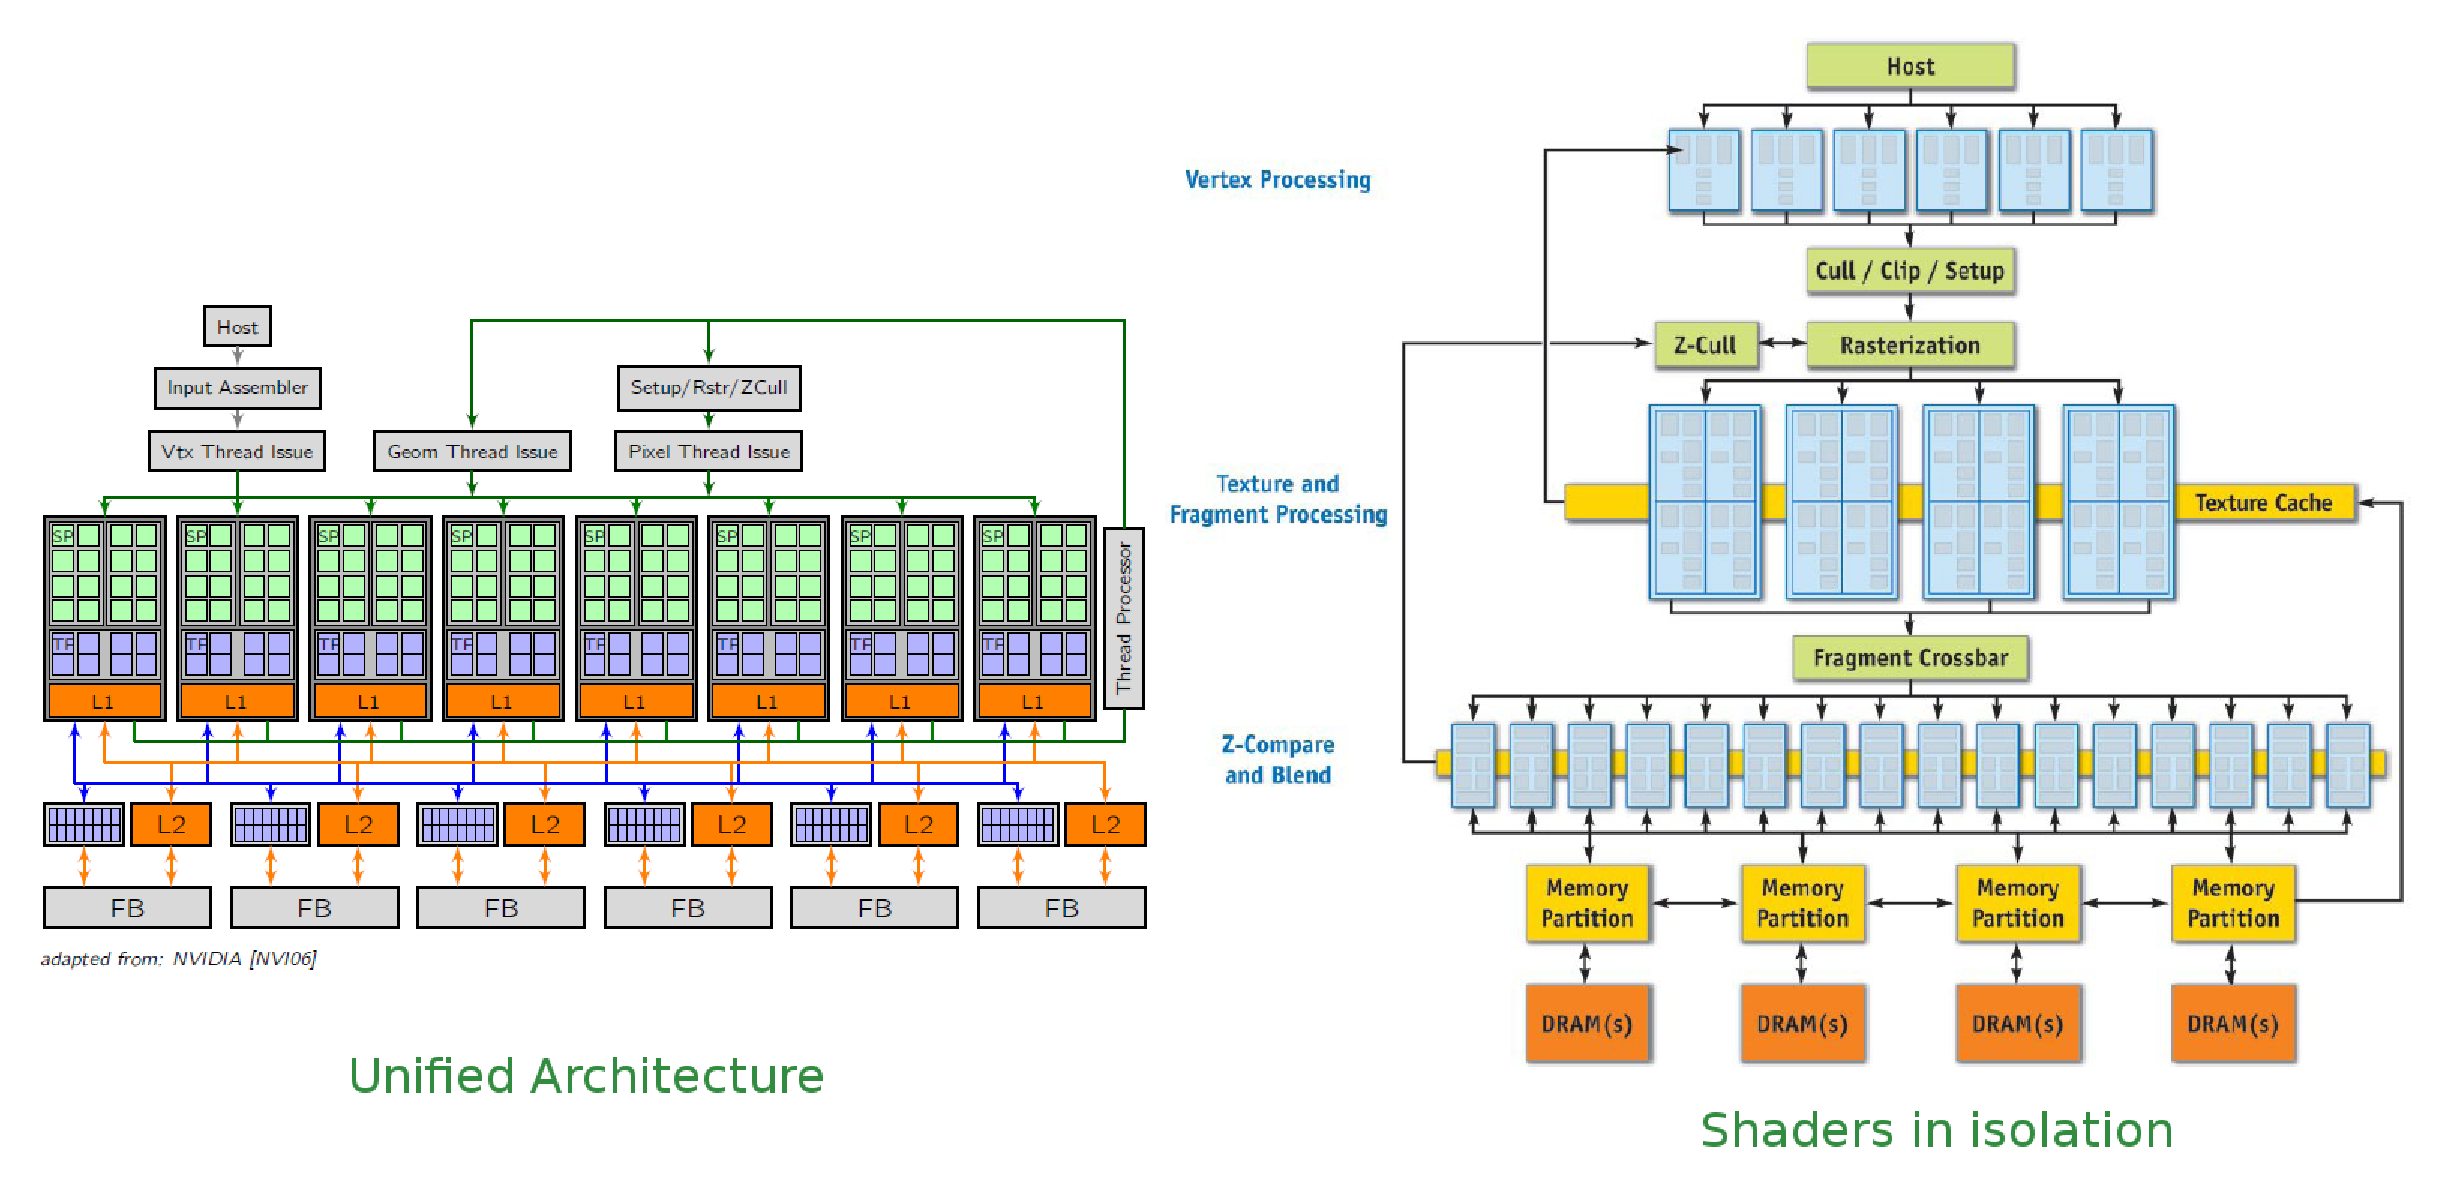
\includegraphics[height=7cm, angle=0]{./images/unified_shaders.eps}}
  \caption{(A) Unified shaders (GeForce 8800); (B) shaders in separate
    (GeForce 6)}
  \label{fig:unified_shader}
\end{figure}

\begin{framed}
  In graphical applications, the speed is more important than the
  precision. So, in G80's chips and earlier, all execution units in
  GPU support only 32-bit operations and don't support 64-bit
  operations. Newer GPU architectures have better support for double-precision
  calculations.
\end{framed}

As you see, a single SP is indeed a quite simple architecture. Nvidia creates a
complete processor, called a {\bf streaming multiprocessor} (SM), by using: 8
SPs, 2 special functional units (SFUs) + 1 multithread instruction fetch and
issue unit (MT issue) + an instruction cache (I cache) + a read-only constant
cache (C-cache) + 16KB read/write shared memory.

At a higher level, 2 SMs, combined with one {\it texture unit} (texture memory
unit TMU) \footnote{texture unit (or texture pipe) to serve 2 SMs to
  balance the expected ratio of math operations to texture operations}
+ one geometry controller (i.e. PolyMorph unit) + one shared-memory
controller (SMC), form a {\bf Thread Processor Cluster} (TPC). All
TPCs, along with L2 texture cache, form the
{\bf Streaming Processor Array} (SPA).

\begin{figure}[hbt]
  \centerline{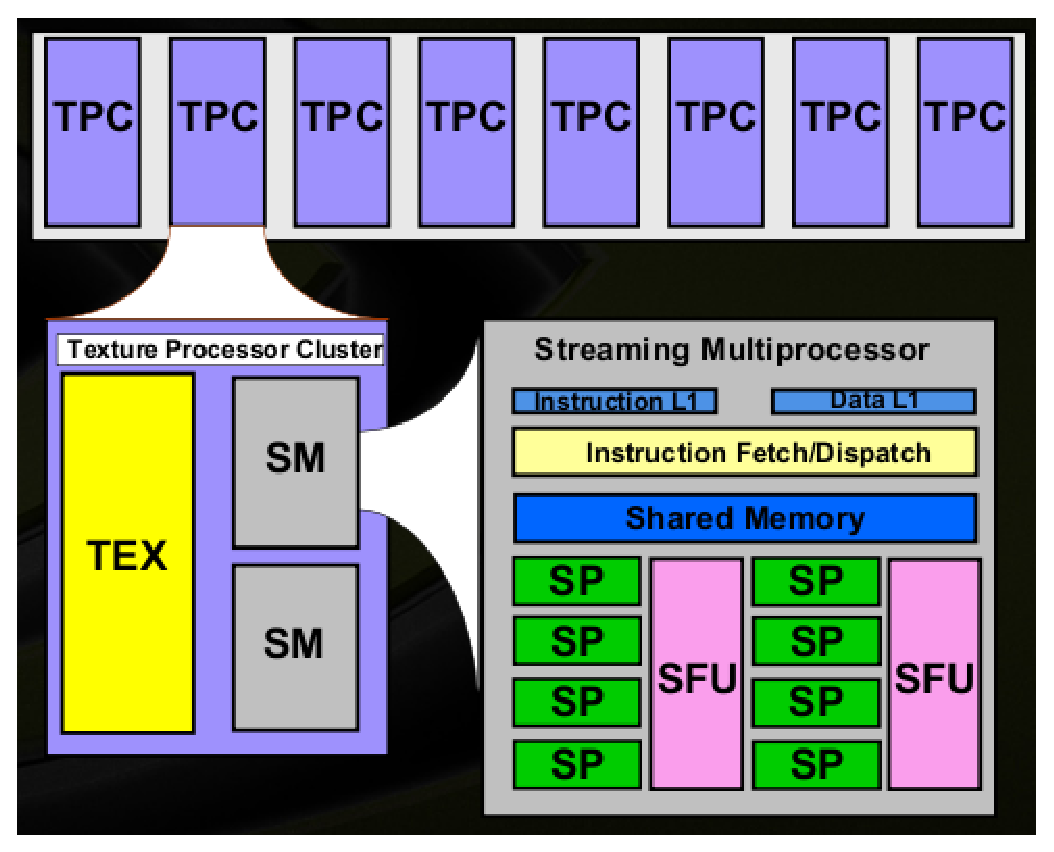
\includegraphics[height=5cm,
    angle=0]{./images/G80_chip.eps}}
  \caption{SPA, TPC, SM, SP in G80}
  \label{fig:G80_chip}
\end{figure}

G80, with 128 processors, has 8 TPCs, Fig.~\ref{fig:G80_chip}.  To
form a complete graphics chip, we still need one execution unit in
GPU, known as a fixed-function {\it raster operation processor} (ROP)
that do the final work of by generating a raster
picture\footnote{\url{http://en.wikipedia.org/wiki/Raster_graphics}}
by writing batches of fragments to framebuffer (FB) memory to display
on the monitor
\footnote{\url{http://ixbtlabs.com/articles3/video/cuda-1-p3.html}}.
In G80s chip, there are 6 ROP partition and six 64-bit FB memory
controllers (i.e. $6\times 64=384$-bit bandwidth). Each ROP partition
has 4 ROP units, i.e. G80s chip has 24 ROP units.


The input information, i.e. color and depth values, are transferred
via an interconnection network. This network also routes the texture
memory read requests from SMs to DRAM and read data from DRAM through
L2 texture cache back to SMs.  The input of the SMs is the coordinate
information of the pixel/vertex, then does the computation to find the
color\footnote{\url{http://www.realworldtech.com/page.cfm?ArticleID=RWT090808195242&p=10}}.

\begin{framed}
  In CUDA, SMs can process vertex, geometry, and pixel-fragment shader
  programs and parallel computing functions (kernels).
\end{framed}

\subsection{GT200 (T10 architecture)}
\label{sec:gt200-1}

The major changes are, as shown in Fig.\ref{fig:T10_arch}(A)
\begin{enumerate}
\item second generation SP use 55nm technology $\rightarrow$ more SPs
  (from 128 to 240), i.e. 10 TPC, each TPC has 3SMs

\item second generation SM: add one 64-bit arithmetic unit (to process
  double-precision) per SM, i.e. DP-based computation is 1/8 of
  SP-based computation in performance. With DP support, and running at 
  1.3GHz, it can do 1 TFLOP SP, and 86.4 GFLOP DP.
\item Each TPC is 3 SMs, rather than 2. 
\item Faster bandwidth, use 512-bit interface, i.e. 102GB/s bandwidth.

\end{enumerate}

\begin{figure}[hbt]
  \centerline{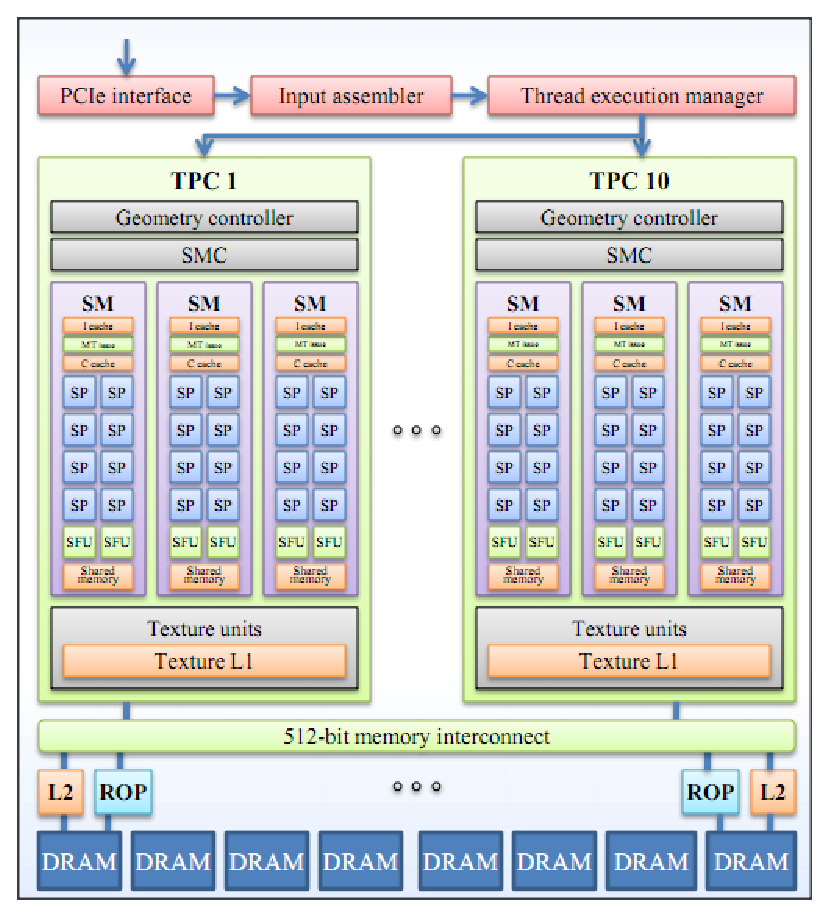
\includegraphics[height=5cm,
    angle=0]{./images/T10_Tesla.eps}; 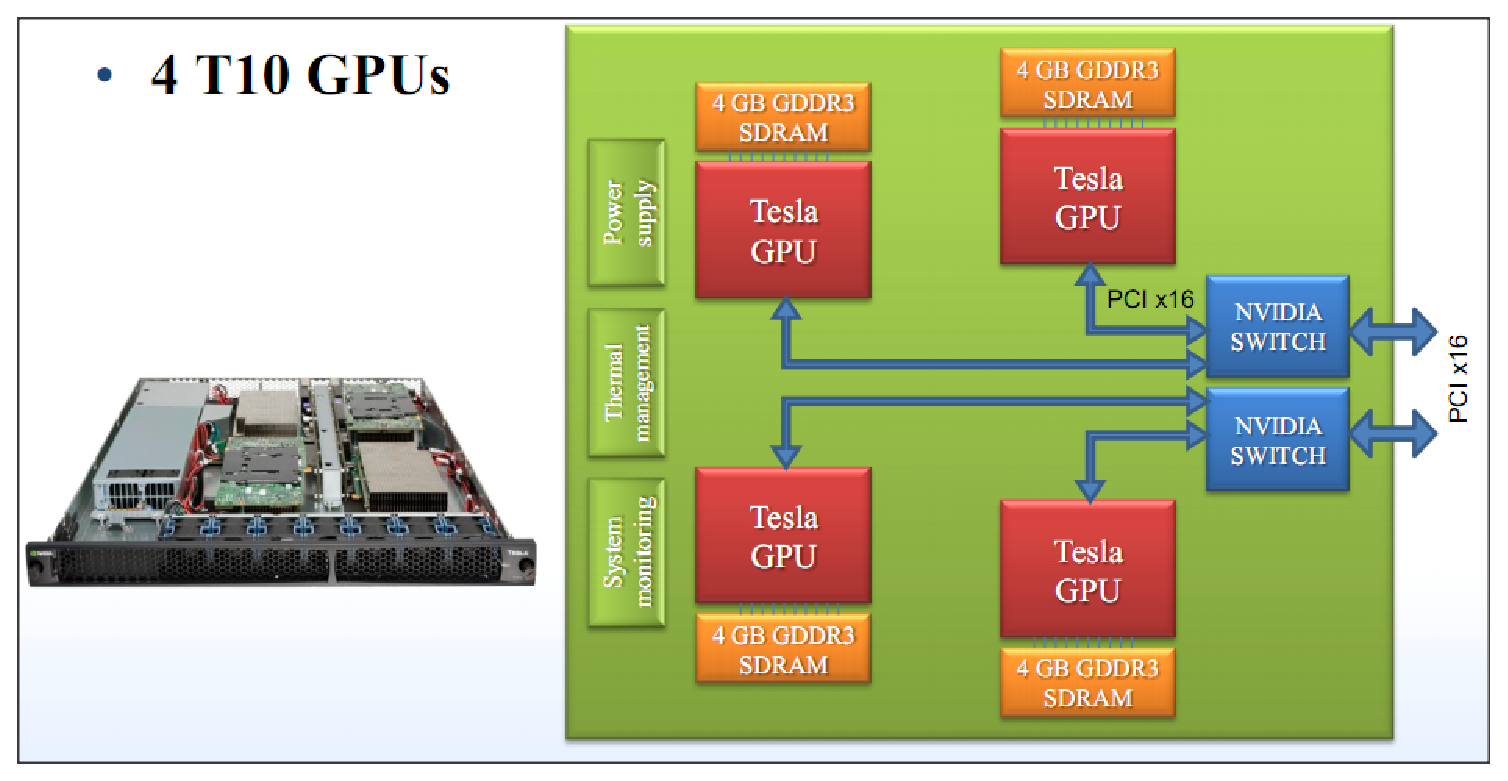
\includegraphics[height=5cm,
    angle=0]{./images/S1070.eps}}
\caption{(A) T10 architecture (GT200); (B) S1070 GPU Computing Server}
\label{fig:T10_arch}
\end{figure}

S1070 is the device with 4 chip T10, connecting to the system with 2 PCIe-x16
bus. Each two T10 chips connect to one PICe-x16 using an Nvidia switch,
Fig.\ref{fig:T10_arch}(B).
% Fig.\ref{fig:S1070}.
% 
% \begin{figure}[hbt]
%   \centerline{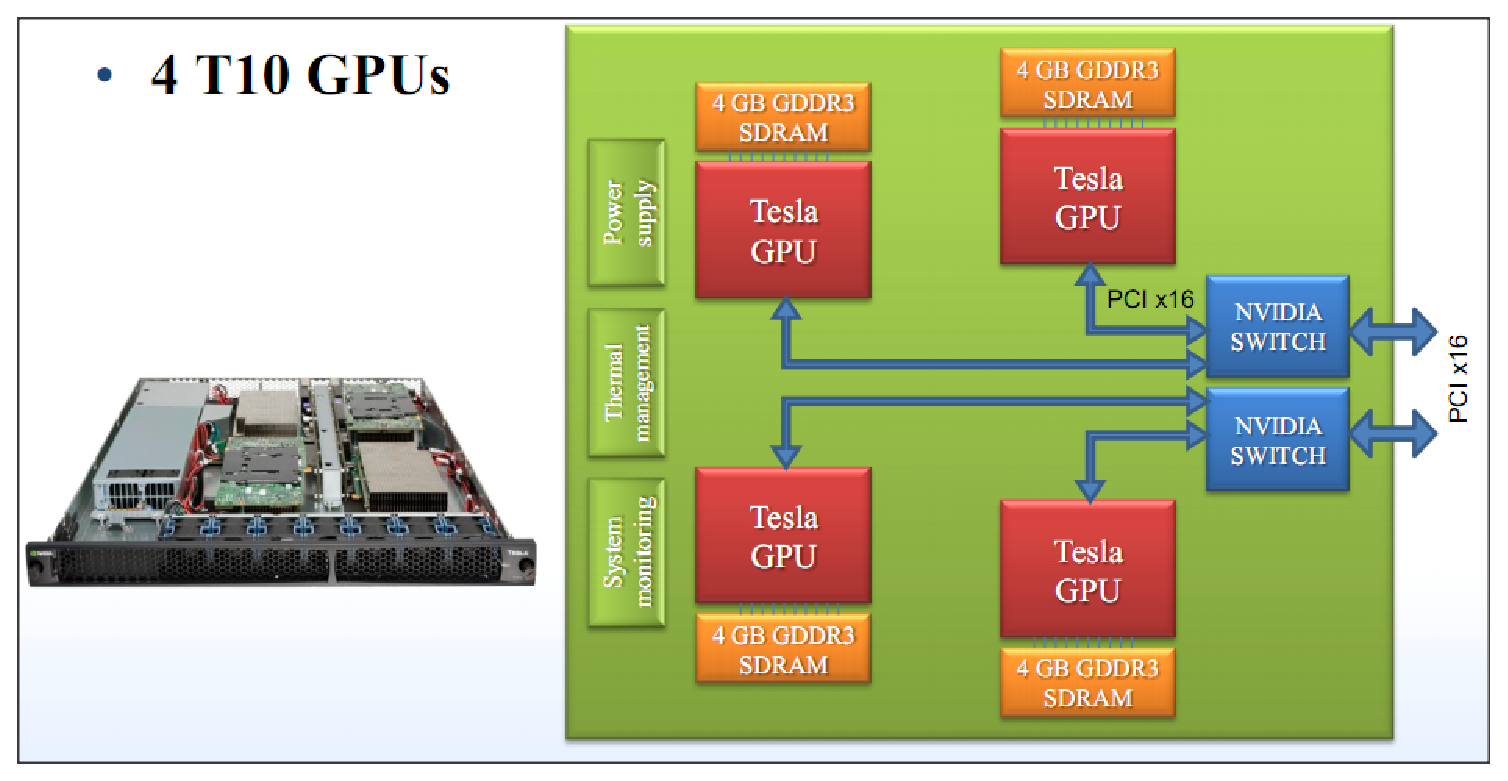
\includegraphics[height=5cm,
%     angle=0]{./images/S1070.eps}}
% \caption{S1070 GPU Computing Server}
% \label{fig:S1070}
% \end{figure}

\section{Tesla 3 (Fermi) GPU}

Tesla 3 (widely known as Fermi) is C2050 which use GF100 chip.

\subsection{GF100 (Fermi)}
\label{sec:gf100-fermi}

SUMMARY: GF100 uses memory interface    320-bits; memory bandwidth 133.9 GB/s;
core clock 607.5 MHz and processor    clock 1215 MHz while memory clock 837MHz (3348 MHz
effective data rate).    GRAPHICS: 56 texture units; 40 raster operators (ROP);
texture fill rate 34    billion/sec; pixel fill rate: 24.28 GPixel/s; 3-way SLI
support.


\begin{figure}[hbt]
  \centerline{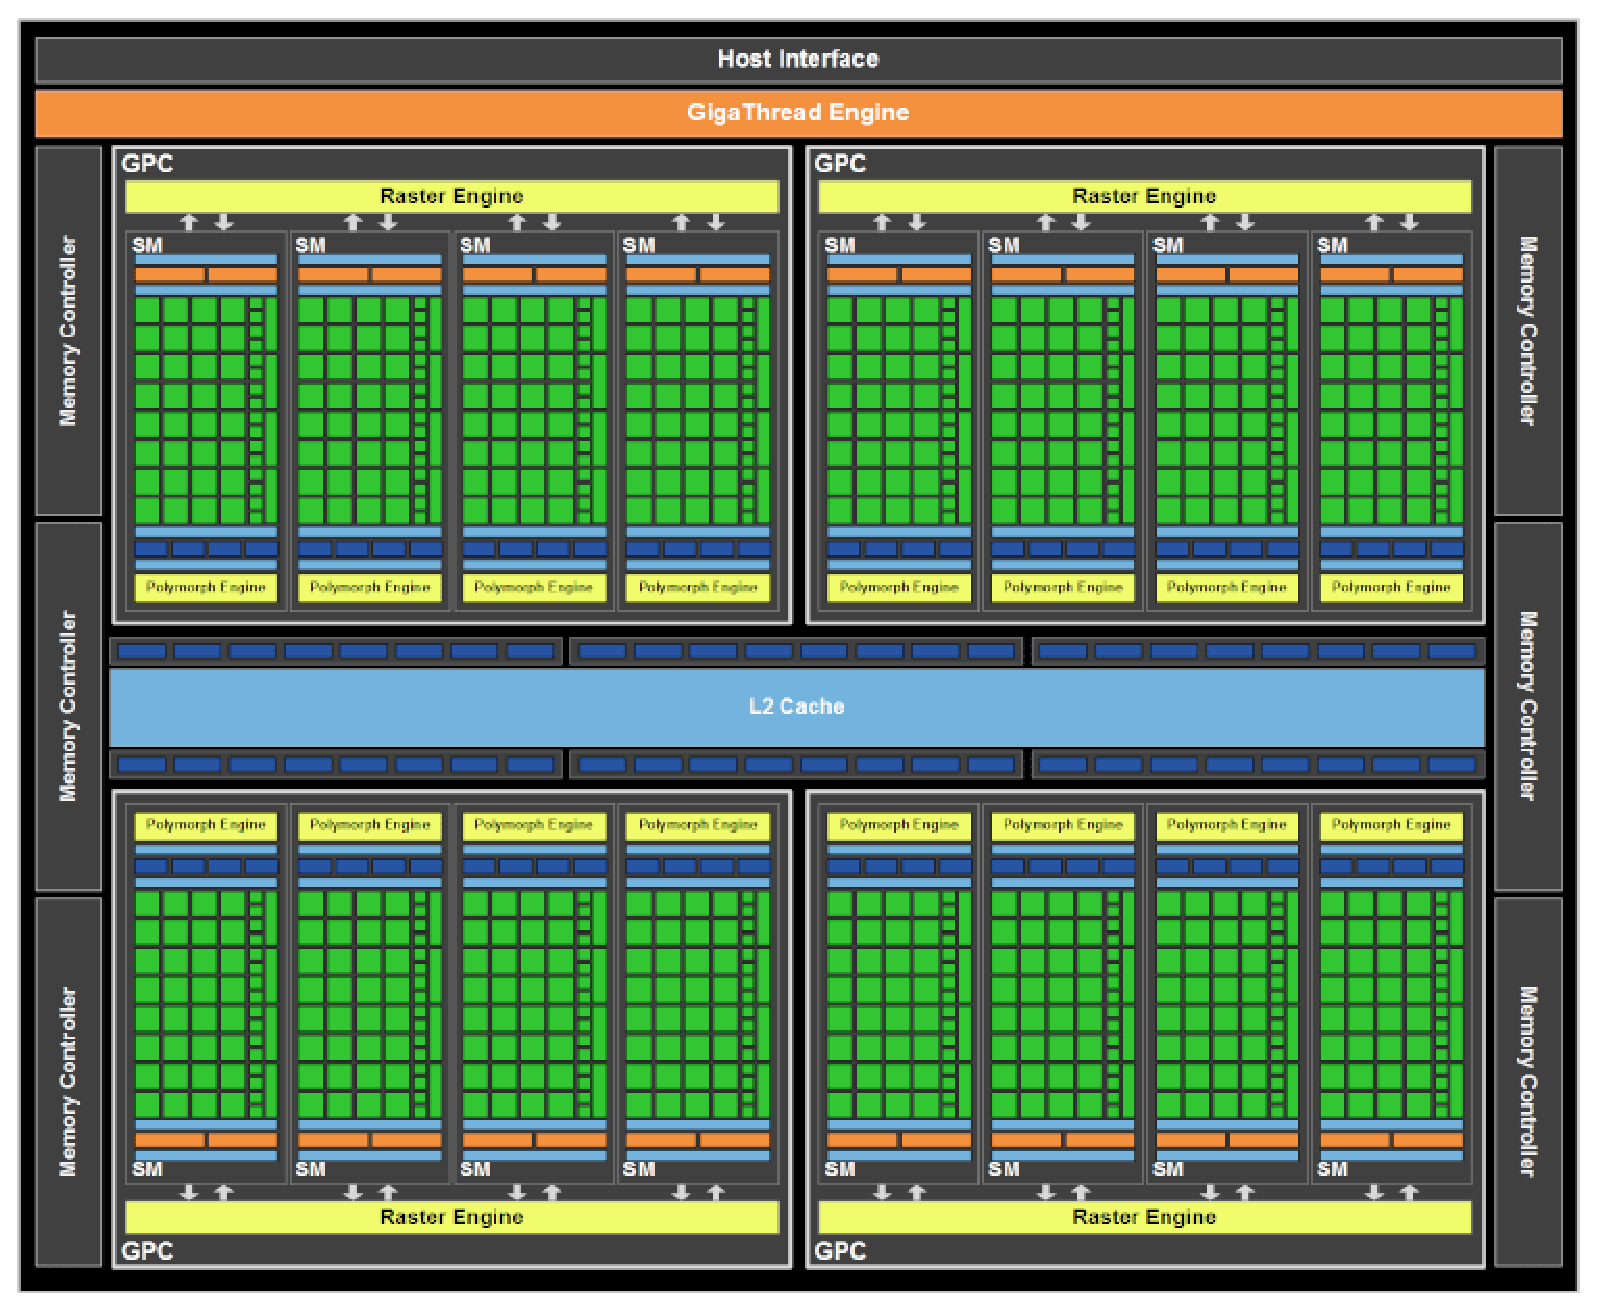
\includegraphics[height=7cm,
    angle=0]{./images/gf100.eps}; 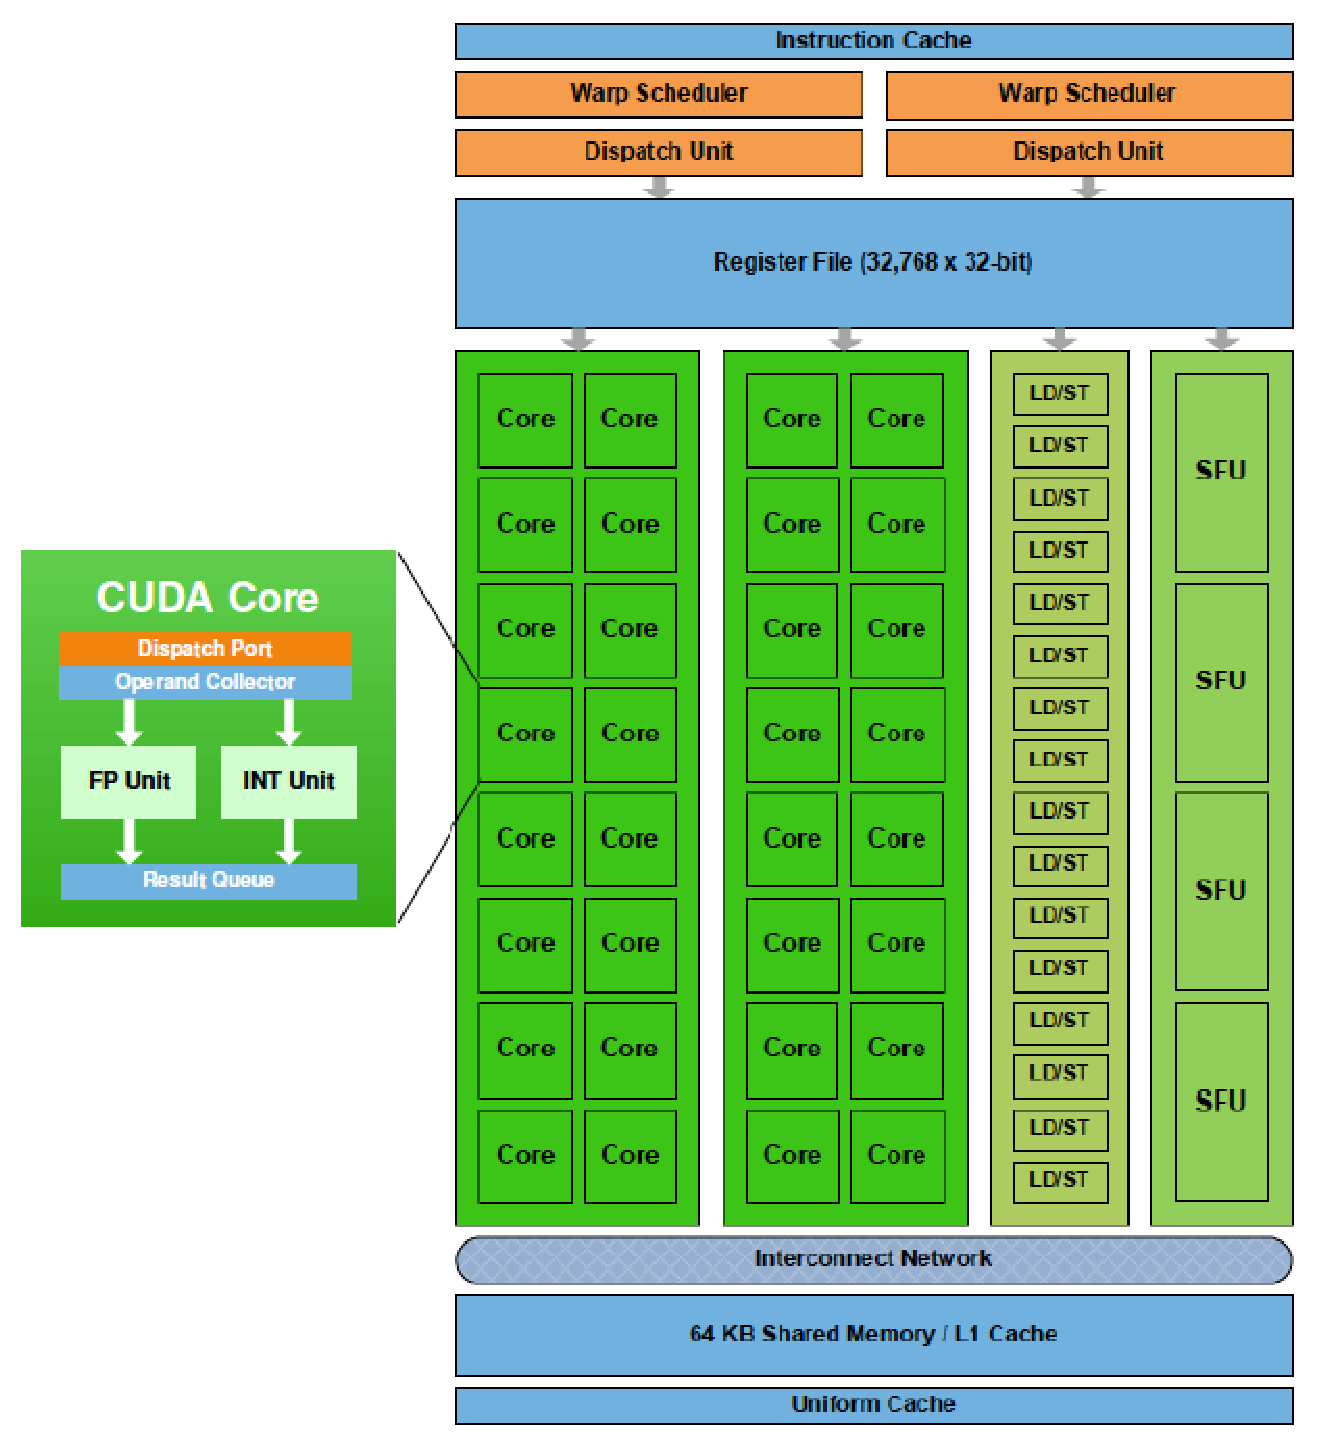
\includegraphics[height=7cm,
    angle=0]{./images/gf100_sm.eps}}
\caption{(A) Diagram of GF100 chip; (B) An SM in GF100}
\label{fig:gf100}
\end{figure}

% \begin{figure}[hbt]
%   \centerline{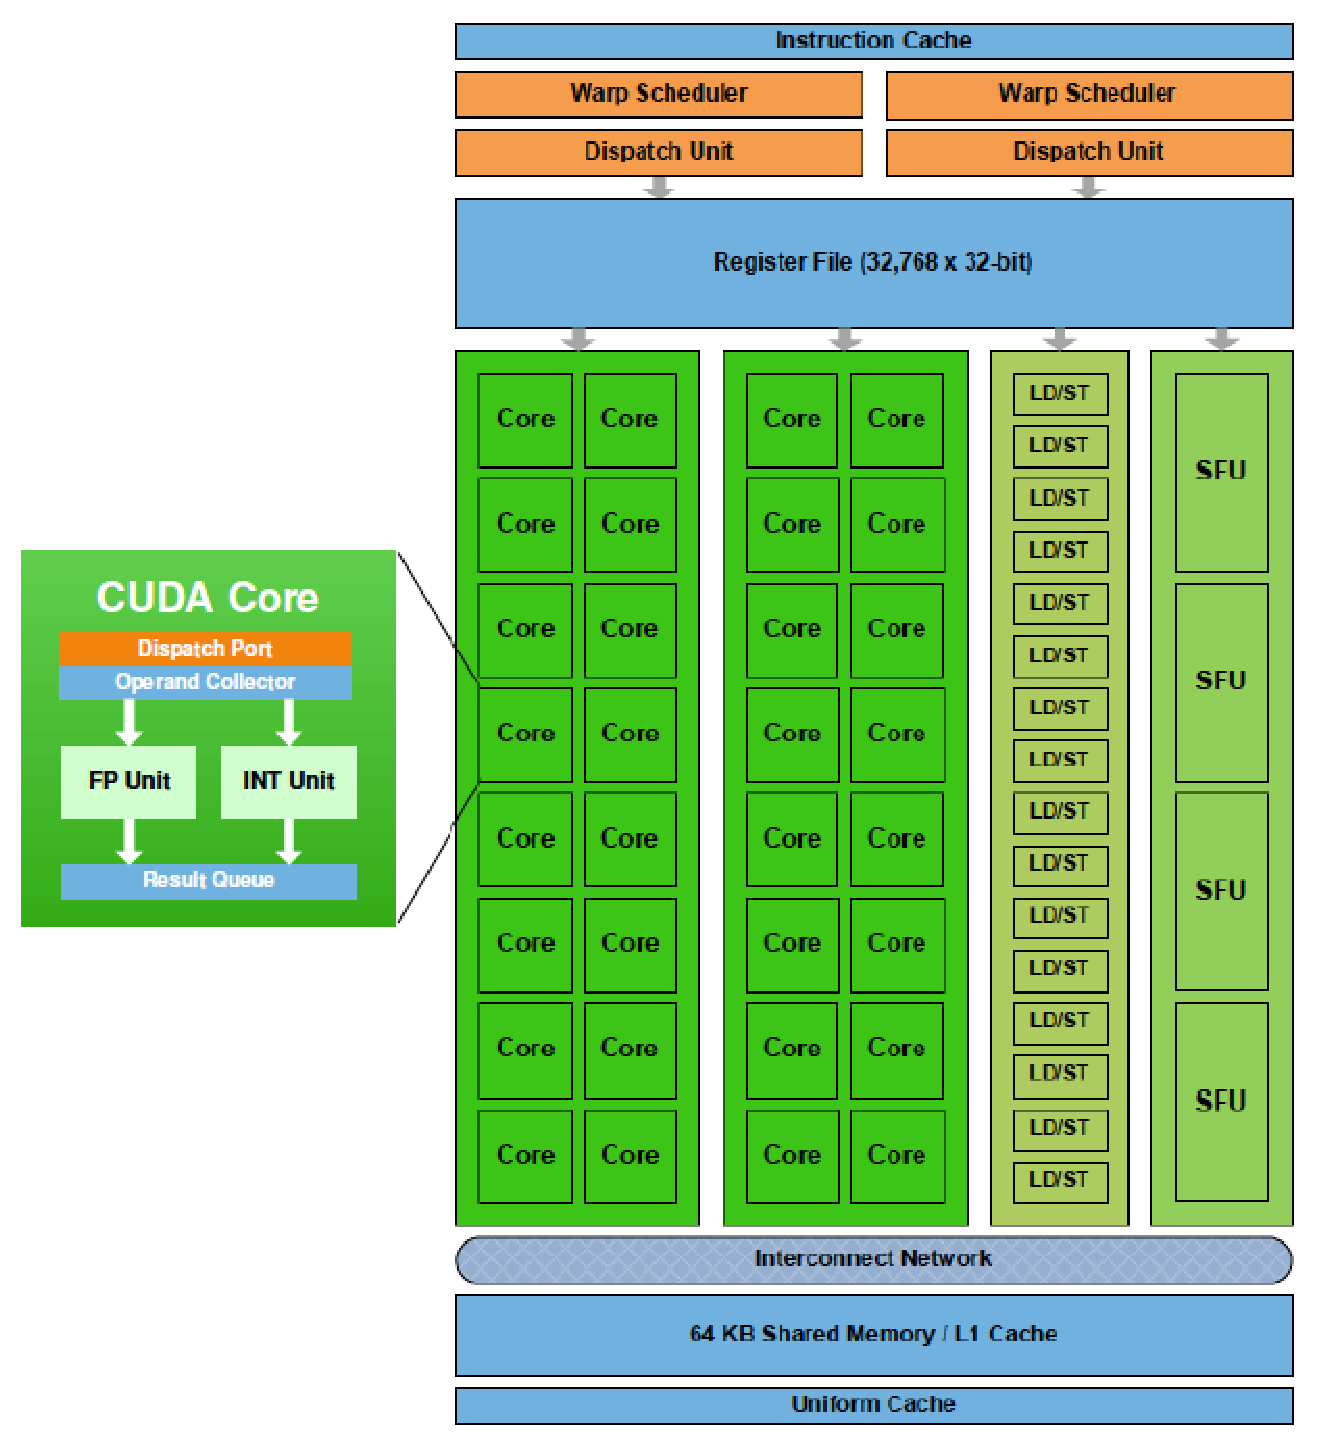
\includegraphics[height=10cm,
%     angle=0]{./images/gf100_sm.eps}}
% \caption{A streaming multiprocessor (SM) in Fermi (GF100)}
% \label{fig:gf100_sm}
% \end{figure}

There are many major changes in Fermi architecture, Fig.\ref{fig:gf100}. 
\begin{enumerate}
\item The GPU is orgnized into a number of GPC. The architecture of a single GPC
in GF100 is given in Fig.\ref{fig:Fermi_GPC}.

\item third generation SM in GF100 has 32 SPs and other stuffs, as shown in
Fig.\ref{fig:gf100}(B).

\item third generation SP use 40nm technology, now has a fully
  pipelined arithmetic logic unit (ALU) and floating point unit
  (FPU). It gives more SPs per chip (i.e. 512 SPs or 16 SMs or 4 GPCs)

  \begin{framed}
    Due to the limitation in 40nm architecture, Nvidia has to disable
    \begin{itemize}
    \item one SM, i.e. GTX 480 has 15 SMs with 480 CUDA cores
    \item two SMs, i.e. GTX 470 has 15 SMs with 448 CUDA
      core.
    \item a GPC, i.e.  result in a 384 core part with three raster
      engines and 12 PolyMorph engines.
    \end{itemize}
  \end{framed}



% , is
%  composed of one I-cache, 32 SPs + 4 TEX units + 16 load/store units + 4 SFUs +
%  2 warp schedulers with 1 dispatch unit
%   each + 1 Polymorph unit + 48KB+16KB L1 cache, registers, and other glue that
%   brought an SM together.

\item new (true) unified 768KB L2 cache are equally shared by all SMs
\item new shared/L1-cache memory configurable architecture (in 48/16KB
  or 16/48KB).
\item support higher accuracy with fused multiply-add (FMA)
  instruction
\item higher throughput in overall (memory, computational power,
  context switching...)
\item execute multiple task kernels at once

\item revise geometry units: PolyMorph units + Raster Engines
  \begin{itemize}
  \item 16 PolyMorph units (geometry units): each does 5 stages
    (Vertex Fetch, Tessellation, Viewpoint Transform, Attribute Setup
    and Stream Output) and serves a single SM. 
  \item 4 Raster Engines: each does 3 stages (Edge Setup, Rasterizer,
    Z-cull) and serves 4 SMs.
  \end{itemize}


  \begin{framed}
    Nvidia realizes that pure geometry performance increases only 3x
    from GFX5900 to GTX285, while pixel shading performance has
    increased by 150x. The reason is that geometry shading and
    tessellation requires a lot of works from the SM units in general,
    and data is frequently passed between SM and PolyMorph Engine, at
    different stages of rendering. So, Nvidia decided to bring
    PolyMorph unit closer to SMs, and add a separate hardware unit to
    do Tessellation - the Tessellator - to the PolyMorph
    engine. Nvidia expects to see a near 4x+ improvements in
    tessellation performance compared to AMD/ATI Radeon HD 5870.
  \end{framed}

  \begin{framed}
    Output of the PolyMorph engines are sent to the Raster Engines
    where it decides which pixels going to be viewed, and which should
    be discarded. After that, post-processing and pixel shading are
    done by the SMs.

  \end{framed}

\item 6 ROP partitions, each ROP partition has 8 ROP units, rather
  than 4. Totally, Fermi has 48 ROPs. 
  \begin{framed}
    For a while, the main bottleneck in graphical applications is the
    shader bound, i.e. not enough shaders. Now, with 512 cores in
    Fermi, it is no longer the issue, but the {\it pixel
      fillrate}.
    This is due to the rise of multi-screen gaming and Nvidia's 3D
    Vision. To increase the capabilities of pixel fillrate, Nvidia add
    more ROP units per partition.
  \end{framed}

\end{enumerate}

Another advances in software aspect is
\begin{enumerate}
\item C++ language support
\item better debugging support (Nvidia's Nexus plug-in in Microsoft
  Visual studio)
\item compatible with DirectX 11, OpenGL 3.x and OpenCL 1.x 
\end{enumerate}



\subsection{GF104/GF106/GF108}
\label{sec:GF104_GF106_GF108}

SUMMARY: GF104 has smaller memory bandwidth
      256 bits, with fewer CUDA core 384, less raster operators 32; yet more
      texture units 64. To achieve good performance with lesser resources; GF104
      need to run at a higher clock speed (overclocked).
      
The design of GF100 has many flaws inside that Nvidia has to revise it in
different models. One of the main reason to have GF104 is to reduce thermal and
power consumption. Other major changes, Fig.\ref{fig:GF104_100}:
\begin{enumerate}
  \item increase number of cores per SM, from 32 to 48
  \item increase dispatch port per core, from 1 to 2
  \item increase number of dispatch unit per SM, from 2 to 4. So, each warp
  scheduler has 2 dispatch units. 
  \item the number of SFU (special functional units) per SM, from 4 to 8, so it
  can process transcendental functions faster.
  \item texure units per SM, from 4 to 8 which has massive increase in graphical
  applications/games. 
  \item load/store units per SM, from 8 to 16
\end{enumerate}
Each GPC is kept the same with 4 SMs, along with a Polymorph Engines and a
common Raster Engine per
GPC\footnote{\url{http://www.hardwarecanucks.com/forum/hardware-canucks-reviews/34635-msi-geforce-gtx-460-cyclone-768mb-oc-review-2.html}}.
With 2 GPCs in GF104-based GPU, there are totally 2*4*48=384 SPs, 64 texture
units, 32 ROPs, 512KB of L2 cache and four 64-bit memory controllers.

\begin{figure}[hbt]
  \centerline{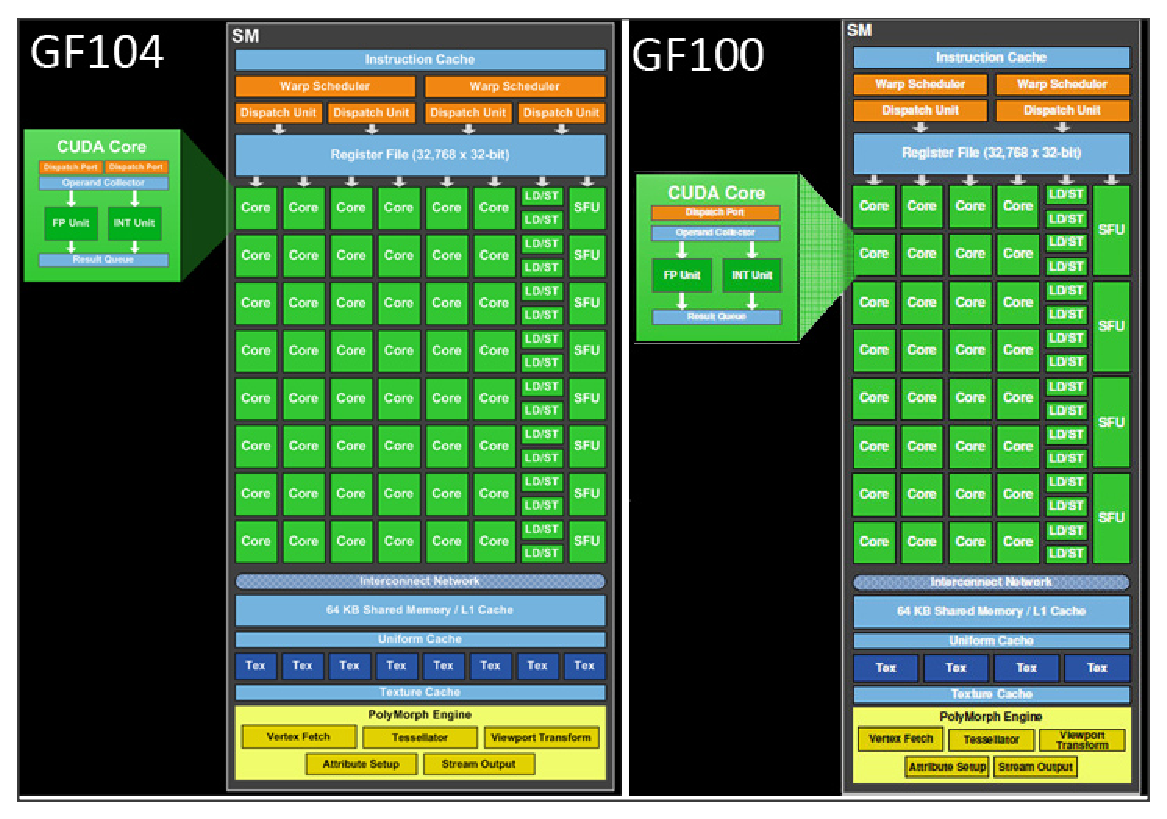
\includegraphics[height=8cm,
    angle=0]{./images/GF104_100.eps}}
\caption{GF104 vs. GF100}
\label{fig:GF104_100}
\end{figure}


\begin{framed}
GF100 use 529mm$^2$ die size. GF104 use 67mm$^2$ die size. The latter is
still 10\% larger than the closest rival, AMD Cypress/HD58xx with 334mm$^2$;
though both chips use the same 40nm
technology\footnote{\url{http://semiaccurate.com/2010/07/21/gf104gtx460-has-huge-die/}}.
GF108 use 130nm$^2$ die size, half of GF106.

GF104 has 1.95 billion transistor, GF100 has 3 billion. GF106 is lower-end and
GF108 is for integrated graphics. GF104 are gts 450,gts 440, gts 430. GF100
are Fermi card, GTX460, GTX48x. GF106 are GTX 445M.
\end{framed}

By increase the number of SPs per SM in GF104, the registers per core is
decreased compared to GF100. Besides, warp scheduler has double instruction
patch units (to 4, rather than 2). The reason for increasing from 32SPs per SM
to 48 SPs per SM (i.. 50\%), but double texture units, is that Nvidia think
tessellation engines is idling too much, so they want to decrease the number of Polymorph Engine per
CUDA core; and increase the shader processing per
PolyMorph\footnote{\url{http://www.pcper.com/reviews/Graphics-Cards/Nvidia-GeForce-GTX-460-Review-GF104-and-budget-Fermi}}.
GF106 has 4 PolyMorph engines (one per SM), and 32 texture units. GF108 tends to
be designed for entry-level cards. 

\subsection{GF110}
\label{sec:GF110}

GF110 is a significant revision from GF100. Fundamentally, GF110 use the same
architecture as GF100, with 32 SPs per SM. They use slower, lower-leakage
transistors in less time-sensitive path, and faster, higher-leakage transitors
in other areas. This allows using lower power and enable the 16th SMs, giving it
full 16 SMs working, i.e. totally 512 CUDA cores. GF110 has improved Z-cull
efficiency and can do FP16 texture filtering in 1 cycle, while GF100 needs 2
cycles\footnote{\url{http://www.tomshardware.com/reviews/geforce-gtx-580-gf110-geforce-gtx-480,2781-2.html}}.
In addition, GF110 use GF104 texture hardware, each unit can compute and fetch 4
32-bit/INT8 texture samples per clock, 4 64-bit/FP16 texture samples per clock
(GF100 can do only 2), and one 128-bit/FP32 texture sample per clock. This will
bring more performance on new games (which utilizes 64-bit texture samples).
\begin{itemize}
  \item  GeForce GTX 480 sported core/shader/memory frequencies of 700/1401/924
  MHz, 
  \item GeForce GTX 580 employs a 772 MHz core clock, a 1544 MHz shader
  frequency, and a 1002 MHz memory clock
\end{itemize}
{\it ``Excessive noise was one of the strongest reasons to avoid GeForce GTX
480, and it is effectively dealt with on the GTX 580.''}

In GF104, each SM can do 32 texels, compard to 96 instruction computed, giving
the ratio 1:3 (NOTE: shader clock is 2x the base (core) clock). In GF100 and
GF110, an SM can do 16 texels, or 64 instruction computed, giving the ratio 1:4 

\textcolor{red}{However, for computational purpose, GF100-based card like C2050
is still the first choice, with ECC memory, handling double-precision at half-rate of single
precision (whirl GF100 can handle double-precision one-quarter of the peak
performance)}.

\begin{framed}
 Z-culling is a method of improving GPU performance by throwing out pixels that
will never be seen early in the rendering process. By comparing the depth and
transparency of a new pixel to existing pixels in the Z-buffer, it's possible to
determine whether that pixel will be seen or not; pixels that fall behind other
opaque objects are discarded rather than rendered any further, saving on compute
and memory resources. GPUs have had this feature for ages, and after a spurt of
development early last decade under branded names such as HyperZ (AMD) and
Lightspeed Memory Architecture (Nvidia), Z-culling hasn't been promoted in great
detail since then. 
\end{framed}
\begin{enumerate}
  \item GF100: has 4
  GPCs\footnote{\url{http://www.tomshardware.com/reviews/geforce-gts-450-gf106-radeon-hd-5750,2734-2.html}}
  \begin{itemize}
    \item GTX 470 (1.25GB): 320-bit bus, bandwidth 133.9 GB/s
    \item GTX 480 (1.5GB): 384-bit bus, bandwidth 177.4 GB/s
  \end{itemize}
  \item GF104: has 2 GPCs, with total 336 shaders (SP or GPU core), with either
  192-bit bus or 256-bit bus
  \begin{itemize}
    \item GTX 460 768MB has 24 ROP units, 384 KB L2 cache, 192-bit bus,
    bandwidth 86.4 GB/s
    \item GTX 460 1GB has 32 ROP units, 512 KB L2 cache, 256-bit bus, bandwidth
    115.2 GB/s
  \end{itemize}
  Each  64-bit memory controller is attached to 8 ROP units.
  \item GF106 (a replacement for G92): has 1 GPCs, with total 1x4x48=192
  shaders, and a 192 bit bus
  \begin{itemize}
    \item GTS 450: 2 ROP units, 32 texture units, 128-bit bus, bandwidth 57.7
    GB/s.
  \end{itemize}
  \item GF108 has 128 shaders and a 128-bit bus. It use DDR3, rather than DDR5
  memory
  \item GF110:
  \begin{itemize}
    \item GTX 580 (1.5GB DDR5): with 512 cores, 64 texture units, 48 ROP units,
    384-bit bus, bandwidth 192.4 GB/s. 
  \end{itemize}
\end{enumerate}


\subsection{ROP}
\label{sec:rop}

{\bf ROP} does the last stage before output the pixel to the console
(screen or printer), e.g.  pixel blending, anti-aliasing, data
compression and other atomic memory operations. That's why the ROP
units interact directly with the global memory (i.e. framebuffer in
graphical term). The performance hasn't been changed (i.e. a single
ROP unit can process one 32-bit integer pixel per
\textcolor{red}{1 clock cycle}, one FP16 pixel over
\textcolor{red}{2 clock cycles}, and one FP32 pixel over
\textcolor{red}{4 clock cycles}); yet the atomic operations are
greatly optimized (i.e. 20x increase in the case of atomic operations
to a single thread, 7.5x for contiguous memory regions...).

\begin{framed}
  In Fermi, the framebuffer (aka the global memory) tie to each ROP
  partition is 64-bit memory bus $\rightarrow$ the chip has $6\times
  64=384$-bit GDDR5 memory bus. Even though it has a lower bit-wide
  than GT200, the rate per pin is double due to Fermi using GDDR5,
  rather than GDDR3. So in overall, it has better memory bandwidth.
\end{framed}

More ROPs capacity means better pixel fillrate (i.e. frame rates) with
higher levels of anti-aliasing, which is always a good
thing\footnote{\url{http://techreport.com/articles.x/14934/7}}.
\begin{itemize}
\item GeForce 7: has 4 ROP partitions, each with 4 ROP units. So
  totally, it has 16 ROP units.
\item G80: has 6 ROP partitions
\item G92: has 4 ROP partitions
\item GT200: has 8 ROP partition 

  In G80, G90, GT200, each ROP partition is composed of 4 ROP units
  and can output 4 pixels per clock.
  \textcolor{red}{ GT200 can draw pixels at a rate of 32 pixels per
    clock cycle}.

\item GF100: has 6 ROP partitions, yet a single ROP partition is
  composed of 8 raster execution units. All execution units share the
  L2 cache with the rest of GF100.

  Like previous generations, each ROP in Fermi can process 1 regular
  32bit pixel per clock, 1 FP16 pixel over 2 clocks, or 1 FP32 pixel
  over 4 clocks. Thus, with 48 ROP units,
  \textcolor{red}{GF100 can process 48 regular pixels per clock}. The
  ROPs are clocked together with the L2 cache.
\end{itemize}

\begin{figure}[hbt]
  \centerline{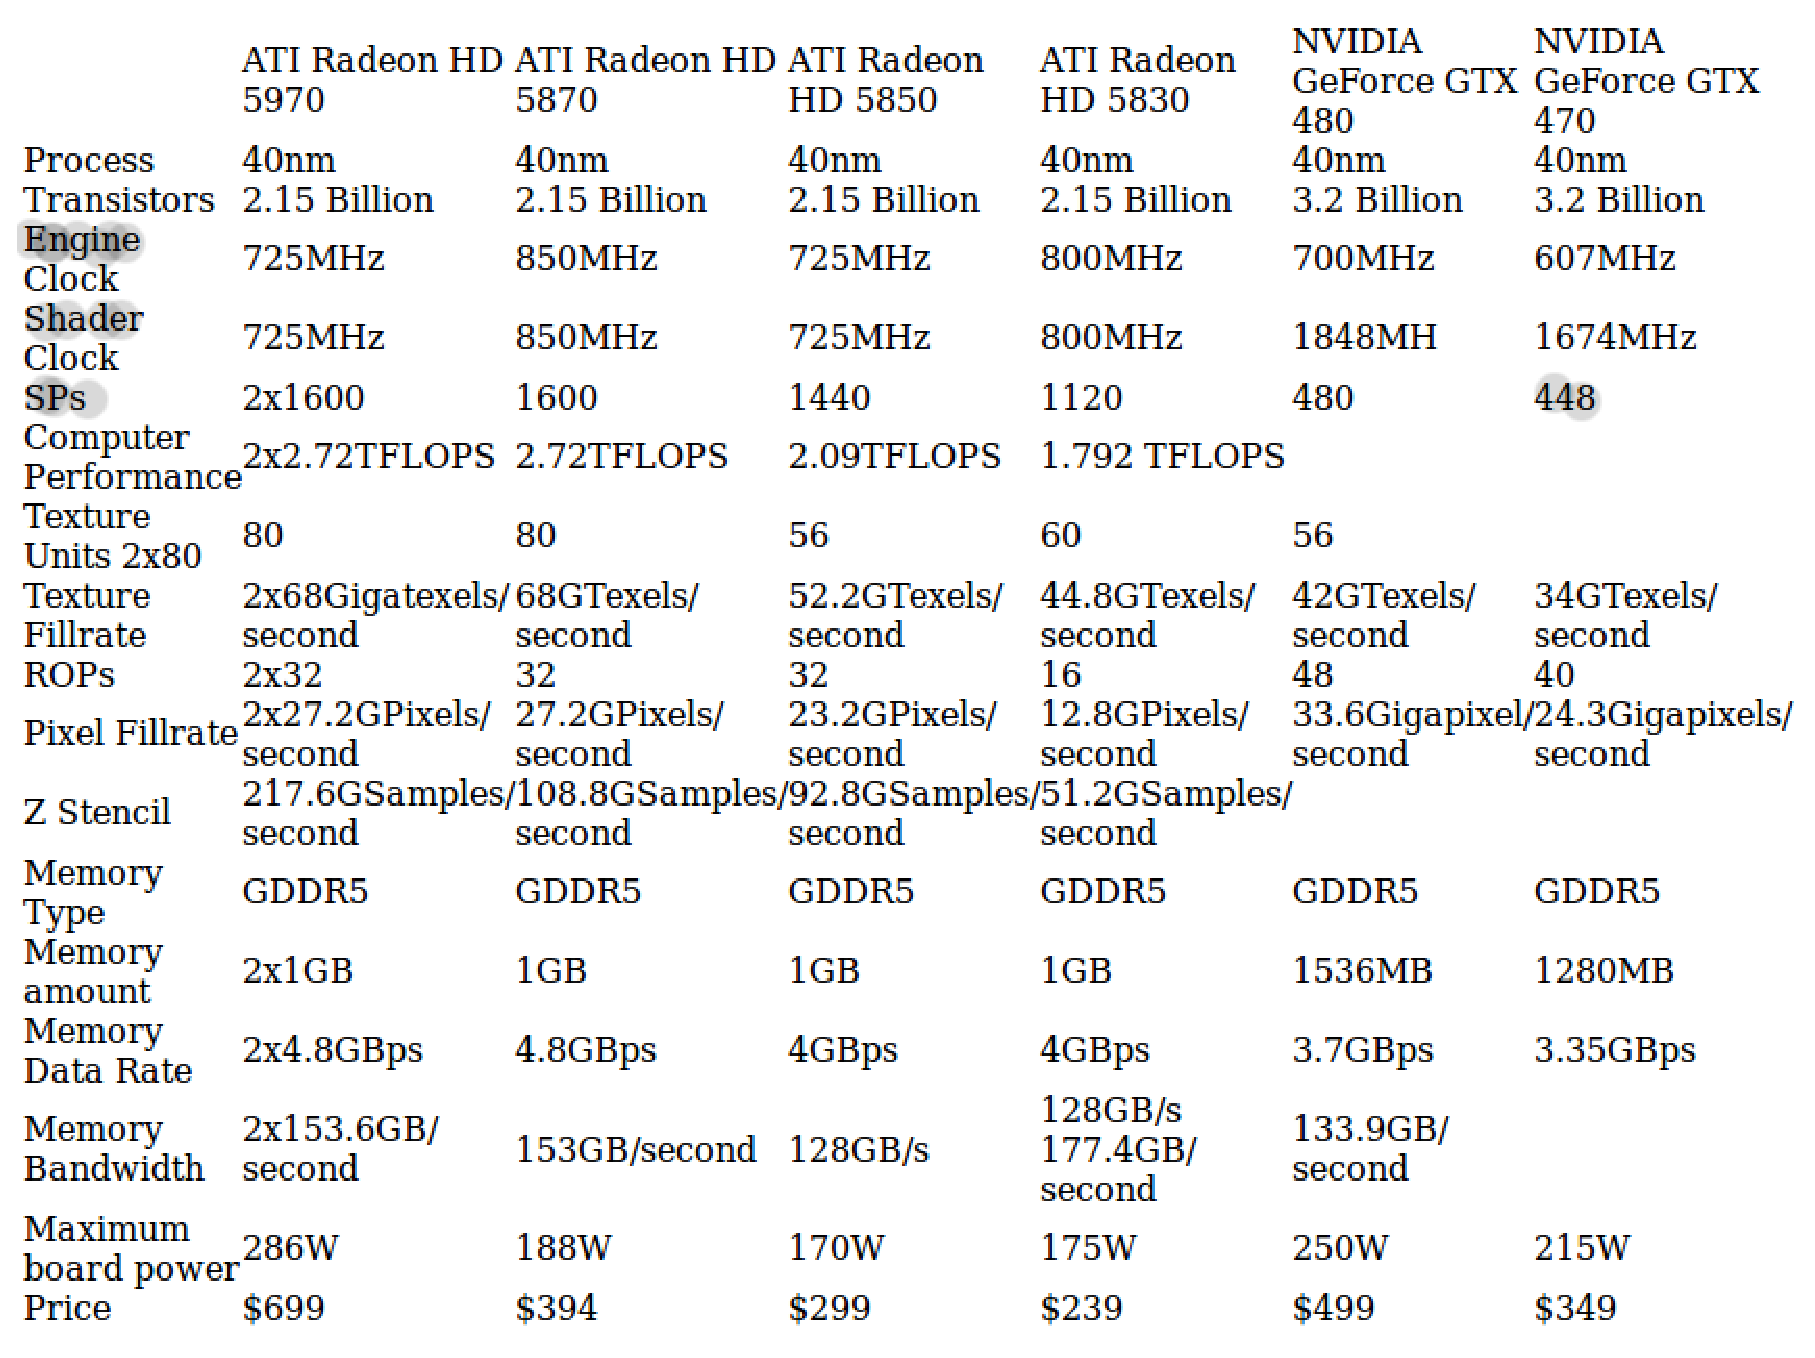
\includegraphics[height=10cm,
    angle=0]{./images/gpu_compare.eps}}
  \caption{GPU comparison}
  \label{fig:GPU_compare}
\end{figure}

The geometric details of the pixel are encoded into the 4
components. {\it Alpha testing} is a per-pixel technique being used to
determine whether to render a pixel to the screen or
not\footnote{\url{http://unity3d.com/support/documentation/Components/SL-AlphaTest.html}}
by comparing the alpha-value against a reference value. To achieve
better visual effect, instead of using render-or-not strategy, a
technique called {\it alpha blending} uses the alpha value to
determine how much the pixel contribute to the final image.  This can
produce soft edges, yet quite slow. {\it Alpha-to-coverage} basically
changes alpha blending into per-sample alpha testing. Another, better
technique is called {\bf transparency supersampling} (TSAA). A faster
but lower-quality anti-aliasing method than TSAA is Transparency
Multisampling (TMAA). The two methods are collectively called
{\it transparency anti-aliasing} and was introduced on the GeForce
7800GTX (G70) to fix issues with {\it alpha to coverage} on DirectX 9
games.

\begin{framed}
  The G70 was a DirectX 9 card and games running on these cards with
  TMAA on can look better. For the most part, TMAA is not a valid
  option as it doesn't really fix billboard aliasing. With the GF100
  and alpha to coverage, TMAA will have higher image quality in games
  that use it. The majority of games released today are still DirectX
  9 based, and TMAA will improve the image as it turns on alpha to
  coverage on DX 9 games.
\end{framed}

To avoid aliasing, (spatial) multi-sampling antialiasing (MSAA) [or
full scene anti-aliasing (FSAA)] technique is widely used in which the
picture is written out to the region of 2x or 4x the display
resolution, then down-sampled to match the display resolution. GeForce
8 support 8x MSAA. In addition, Nvidia also implement a new
anti-aliasing mode called {\it coverage sample anti-aliasing} (CSAA)
that improve the precision, yet only being used in special cases.
CSAA takes the color values of the FSAA such as 4x or 8x and applies
coverage samples to the pixel to smooth out lines without paying the
color sample cost of storage.

\begin{framed}
  More ROPs means the GPU can have better multisample anti-aliasing
  (MSAA) performance, Fig.~\ref{fig:anti_alias}.  The GF100 is expected
  to offer high performance with 8X MSAA, as the chip has more than
  three times the texture sample units of the GT200 and is geared to
  performance with 8X MSAA in mind. By way of comparison, the GeForce
  GT200 chip was architecture with 4x MSAA in mind, as it is limited in
  performance when 8x is enabled
  (8XQ)\footnote{\url{http://www.motherboards.org/reviews/hardware/2038_7.html}}.
\end{framed}

\begin{figure}[hbt]
  \centerline{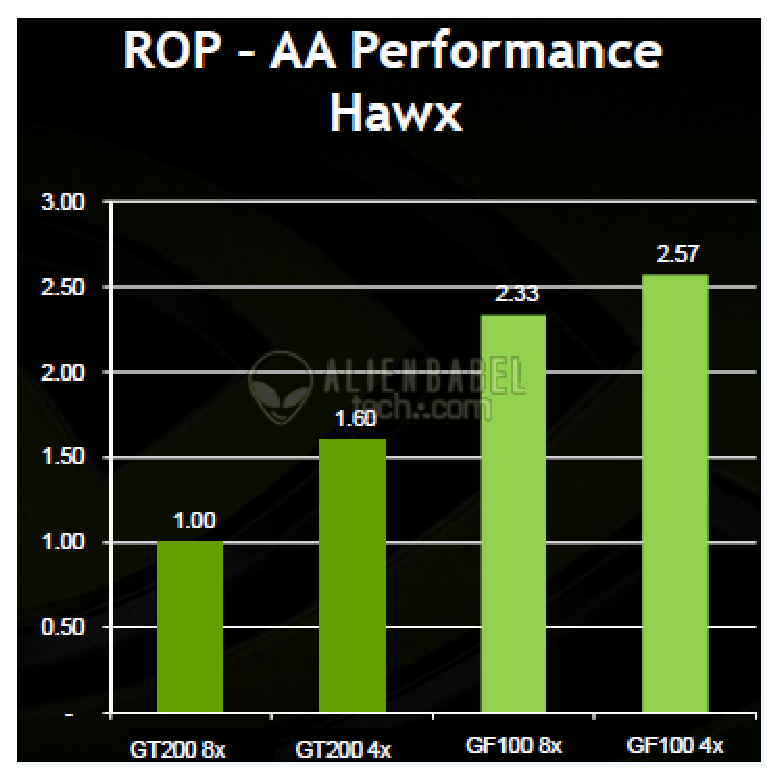
\includegraphics[height=5cm,
    angle=0]{./images/fermi_anti-alias.eps}}
  \caption{Anti-Aliasing (AA) performance comparison}
  \label{fig:anti_alias}
\end{figure}

Instead of using 8x MSAA, GF100 use 32X CSAA, and the possibility of
combining CSAA with MSAA to improve anti-aliasing of transparent
surfaces.. In 32x CSAA, the color values of 8x MSAA is stored with 24
additional coverage samples taken to a give better image quality than
8x by itself. The GF100 supports {\it alpha to coverage}
testing\footnote{\url{http://en.wikipedia.org/wiki/Alpha_to_coverage}}
which can allow the GF100 to blend fences, foliage and other fake
geometry that many games use.
\textcolor{red}{The GF100 can take up to 32 samples per pixel allowing
  up to 33 levels of transparency, compared to the 8 levels on the
  GT200}.


\subsection{Summary}
\label{sec:summary-CUDA_gpu_arch}


\begin{framed}
  The Texture Unit, ROP Unit, PolyMorph Engine and Raster Engine run
  at half the shader clock, rather than at the graphic core
  clock. GF100 is supposed to deliver 8x the geometry performance to
  GT200.
\end{framed}

The picture of GF100 (Fermi) is shown in Fig.~\ref{fig:gf100} (NOTE: 2
SMs are disabled). {\bf A GPC in Fermi has}
\begin{itemize}
\item 4 SMs
\item A Raster Engine. A Raster Engine processes 9 pixels per clock
  i.e.  \textcolor{red}{GF100 can process 32 pixels per clock}.
\item 4 Polymorph Engines
\end{itemize}

{\bf An SM in Fermi has}
\begin{itemize}
\item  32 SPs, instead of 8 SPs like GT200

\item  A Raster Engine. Each SM
  has\footnote{\url{http://www.geeks3d.com/20100118/Nvidia-gf100-architecture-details/}} 

\item 4 Texture units, i.e.
  \textcolor{red}{each GF100 chip has 56 texture units.}
\end{itemize}

\begin{framed}
  A GPC is basically a GPU without ROPs. There are totally 48 ROPs in
  Fermi. 
\end{framed}


References:
\begin{itemize}
\item \citep{lindholm2008ntu}
\item \url{http://www.motherboards.org/reviews/hardware/2038_6.html}
\item \url{http://www.behardware.com/articles/772-6/Nvidia-fermi-the-gpu-computing-revolution.html}
\item \url{http://alienbabeltech.com/abt//viewtopic.php?t=19846}
\item \url{http://www.pcper.com/article.php?aid=888}
\item \url{http://www.behardware.com/articles/644-4/Nvidia-geforce-8800-gtx-8800-gts.html}
\end{itemize}


\section{Tesla 4 (Kepler)}

Tesla 4 (Kepler) that use GK110 chip.




\section{When to use CUDA-capable GPU?}
\label{sec:when-use-cuda}

Recently, Intel has introduced Xeon Phi, a co-processor that use X86 ISA and
there is no need to change to existing codes. To program on CUDA-capable GPU, we
need to modify the codes so that in can run on PTX ISA. Before porting your
software to GPU or writing a new GPU-based software, you need to check the
following requirements for good performance on GPU

\begin{itemize}
\item the software must use a large number of threads

\item there should be a coherence in memory access by device code,
  i.e. data should be laid out to enable coalescing, data accessing
  among threads should have enough locality to use textures or (since
  Fermi) L1 efficiently, e.g. 128bytes cache line... 

\item data transfer between CPU vs. GPU must be minimized, i.e. data
  that are reused between kernels should be kept alive on GPU memory.
  \begin{itemize}
  \item Data on global memory are kept alive between kernels
  \item (since Fermi) Data on L2 cache are kept alive as well
  \end{itemize}

\item Ratio of operations (to be performed on GPU) to elements
  transferred (across CPU-GPU) should be high enough to achieve better
  performance. {\bf Example}:
  \begin{itemize}
  \item Matrices addition requires $3N^2$ elements to be transferred
    and $N^2$ operations (addition); thus the ratio is 1:3 or O(1)
  \item Matrices multiplication requires $3N^2$ elements to be
    transferred and $N^3$ operations (multiply-add); thus the ratio is
    1:N or O(N). 
  \end{itemize}
  As you can see, there is no benefit of using GPU for matrix
  addition; while we can get the benefit with matrices multiplication,
  especially when the matrices size getting larger.
\end{itemize}

\begin{framed}
  Code that cannot be sufficiently parallelized should run on the host,
  unless doing so would result in excessive data transfer between host
  vs. device. 
\end{framed}

The maximum speed-up of a serial program when running on $N$
processors is given by {\bf Amdahl's law}: If a fraction X of
computation is serialized, the speed up cannot be more than (1/(1-X)).
\begin{equation}
  \label{eq:2}
  S = \frac{1}{(1-P) + \frac{P}{N}}
\end{equation}
with $P$ is the fraction of the total serial execution time of the
code that can be parallelized over the total serial execution time of
the whole program. Suppose we have an unlimited number of processors,
then $P/N\approx 0$, or $S=1/(1-P)$. So, if $P=3/4$, we have maximum 4
times speed-up. It means that
\textcolor{red}{we need to spend more time on maximizing the amount of
  code that can be parallelized}.
\chapter{Fermi architecture}
\label{chap:fermi-architecture}

In the previous chapter, we have learnt important concepts of how a GPU work,
comparison between the architecture of a CPU vs. GPU, and a novel programming
model on Nvidia GPU, targetting to high-performance computing applications,
called CUDA. The main components of a CUDA-capable are streaming multiprocessors
(SMs, ranging several to tens) and global device memory.
Nvidia has developed the CUDA-enable GPU to a better design called Fermi
architecture, Fig.\ref{fig:summary_GPU}. We will discover in details in this
chapter. The design and architecture of a SMs can change from generation to
generation (e.g. Tesla 2 has 24 SPs per SM, GF100/GF100 has 32 SPs per SM, GF104
has 48 SPs per SM).

\begin{figure}[hbt]
  \centerline{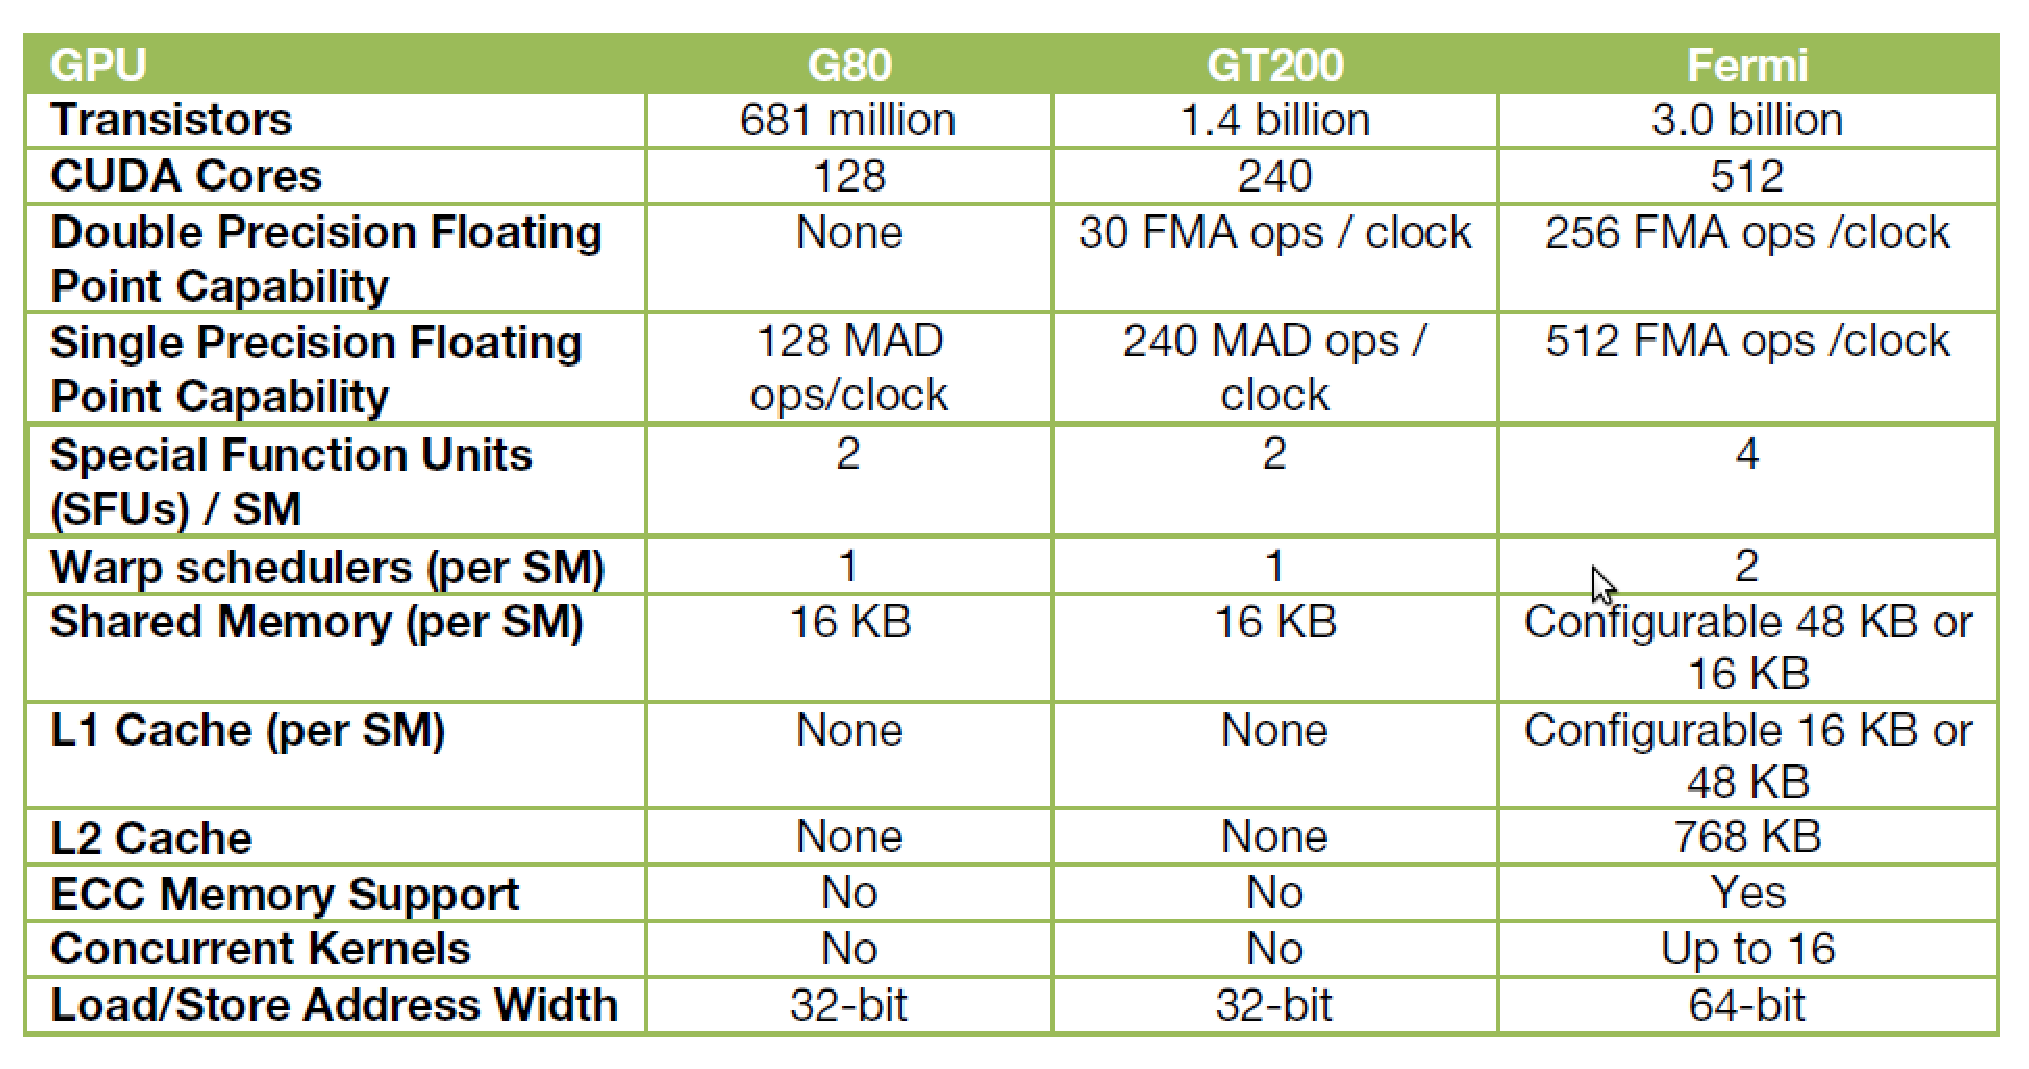
\includegraphics[height=5cm,
    angle=0]{./images/summary_GPU.eps}}
  \caption{Summary of CUDA-capable GPUs}
\label{fig:summary_GPU}
\end{figure}

Fermi is designed to improve performance upon Tesla (GT200) GPUs with special
emphasis on geometry, tessellation, and compute performance for DirectX 11.
\begin{enumerate}
  \item GeForce 256 (1999) has hardware transform and lightning.
  \item GeForce 3 (2001) has programmable shading
  \item GeForce FX has full 32-bit floating-point units
  \item GeForce 8 (2006) introduced unified, scalar shader design (CUDA)
  \item GeForce GTX 480 (GF100 = Fermi) ?????
  \item GeForce GTX 460 (Little Fermi)
  \item GeForce GTX 580 (Fermi Refined)
\end{enumerate}
 
\begin{figure}[hbt]
  \centerline{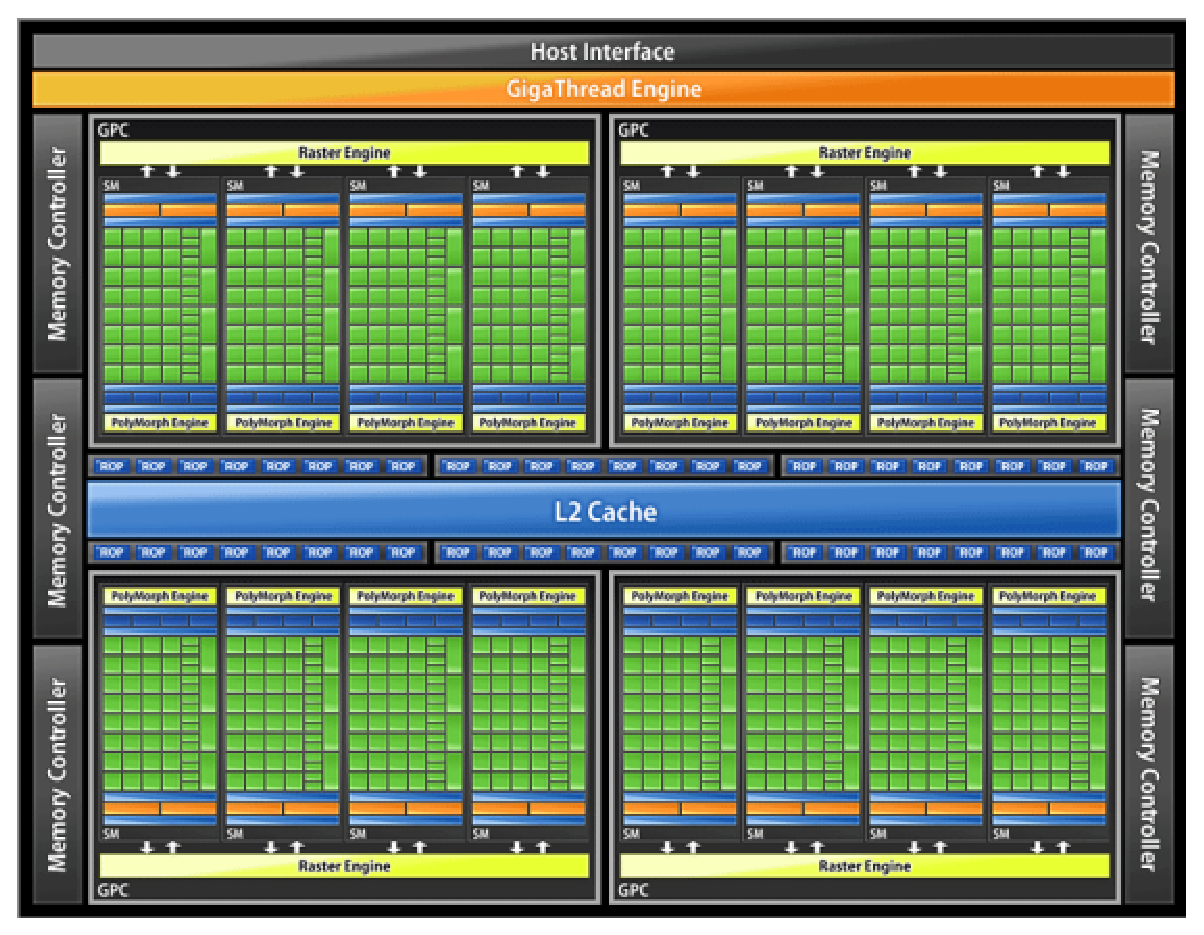
\includegraphics[height=8cm,
    angle=0]{./images/Fermi_C2070.eps}}
  \caption{Nvidia Fermi C2070}
  \label{fig:Fermi_C2070}
\end{figure}


CUDA integration allows full use of Visual Studio source-code
editors, inspectors, debuggers, profilers, and other productivity
features.  

Because Fermi fully supports exception handling at the hardware level,
programmers can set breakpoints in their CUDA source code and single-step
through a program while debugging using \verb!cuda-gdb!.  Visual Studio with
CUDA is currently in beta release.  To support debugging in prior GPUs, traps,
breakpoints or single-stepping first freeze the entire GPU state, and then the
CPU-based debugger reads and writes GPU thread registers, thread state, and GPU
memory over the link between system memory and GPU memory. The CPU based
debugger then resumes GPU execution.


In Fermi, two warps from different thread blocks (even different
kernels) can be issued and executed concurrently, increasing hardware
utilization and energy efficiency.

At any one time, the entire Fermi device is dedicated to a single
application. Fermi supports simultaneous execution of multiple kernels
from the same application, each kernel being distributed to one or
more SMs on the device.

Switching from one application to another is about 20 times faster on
Fermi (just 25 microseconds) than on previous-generation GPUs.


Like earlier GPUs, the Fermi architecture provides for local memory in
each SM.  New to Fermi is the ability to use some of this local memory
as a first-level (L1) cache for global memory references. The local
memory is 64K in size, and can be split 16K/48K or 48K/16K between L1
cache and shared memory.  The decision to allocate 16K or 48K of the
local memory as cache usually depends on two factors: how much shared
memory is needed, and how predictable the kernel's accesses to global
memory (usually the off-chip DRAM) are likely to be.
A larger shared-memory requirement argues for less cache; more frequent or
unpredictable accesses to larger regions of DRAM argues for more
cache.


Each Fermi GPU is also equipped with an L2 cache (768KB in size for a
512-core chip). The L2 cache covers GPU local DRAM as well as system
memory.


The final stage of the local memory hierarchy is the GPU's directly
connected DRAM. Fermi provides six 64-bit DRAM channels that support
SDDR3 and GDDR5 DRAMs. Up to 6GB of GDDR5 DRAM can be connected to the
chip for a significant boost in capacity and bandwidth over NVIDIA's
previous products.

Fermi is the first GPU to provide ECC (error correcting code)
protection for DRAM; the chip's register files, shared memories, L1
and L2 caches are also ECC protected. The level of protection is known
as SECDED: single (bit) error correction, double error
detection. SECDED is the usual level of protection in most ECCequipped
systems. Instead of each 64-bit memory channel carrying eight extra
bits for ECC information, NVIDIA has a proprietary (and undisclosed)
solution for packing the ECC bits into reserved lines of memory.

The total size of the registers (16 * 128 KB = 2048 KB) is larger than
the total size of the L1 caches (16 * 48 KB = 768 KB), and the total
size of the L1 caches equals the L2 cache size (768 KB)

Even though G80 had atomic instructions, the instructions operate on global
memory data. Since Fermi, by allowing these atomic values to be placed in the
shared L2 cache, atomic instructions can be 5X to 20X faster
(Sect.\ref{sec:atomic-functions}).


\section{Overview Fermi}
\label{sec:fermi_overview}

Fermi is designed based on 40nm technology, with 3.0 billion transistors. 

\subsection{Hardware specification of a Fermi GPU}
\label{sec:hardware-information}

In general, a Fermi-capable GPU has, as shown in Fig.\ref{fig:Fermi_C2070}.
\begin{enumerate}
  \item one Host Interface
  \item one GigaThread Engine
  \item 6 memory controllers, each is 64-bit GDDR5 1566 MHz
  \item 768 KB L2-cache shared by all CUDA cores
  \item CUDA cores are grouped into 4 GPC (Graphics Processing Clusters)
\end{enumerate}
Due to design challenge, there are different versions of Fermi-capable GPU, with
one or two SM disabled, e.g. GTX 470 and GTX 480, Fig.\ref{fig:gtx480_470}.
NVIDIA M2050 is a workstation level version of GTX 470 with 448
cores. C2050 is similar to M2050, except with a lower memory bandwidth
(144GB/sec compared to 148 GB/sec). The 1U server (2x M2050) or 4U
tower (4x C2050) enhance dramatically the performance.  

NOTE: A rack is typically 19-inch and 23-inch rack frames, which is about 42U high.

If $n$ is the number of rack units (i.e. $n$U), then the ideal panel height is 
\begin{equation}
h = (1.752n - 0.031)
\end{equation}
or the maximum rack units can be accomodated in a rack of $h$ U is
\begin{equation}
n_{\max} = (h + 0.031)/1.752
\end{equation}
So: $h = 42$, then $n \le 23.9$.

NOTE:
\begin{verbatim}
    Dimension (W x H x D)
1U    19" x 1.75" x 17.7"    (full-(width)-rack, but 1 unit height)
    19" x 1.75" x 19.7"
    19" x 1.75" x 21.5"
    
4U    19" x 7" x 17.8"    (half-rack, but 4 unit height)
    19" x 7" x 26.4"
\end{verbatim}



\begin{figure}[hbt]
  \centerline{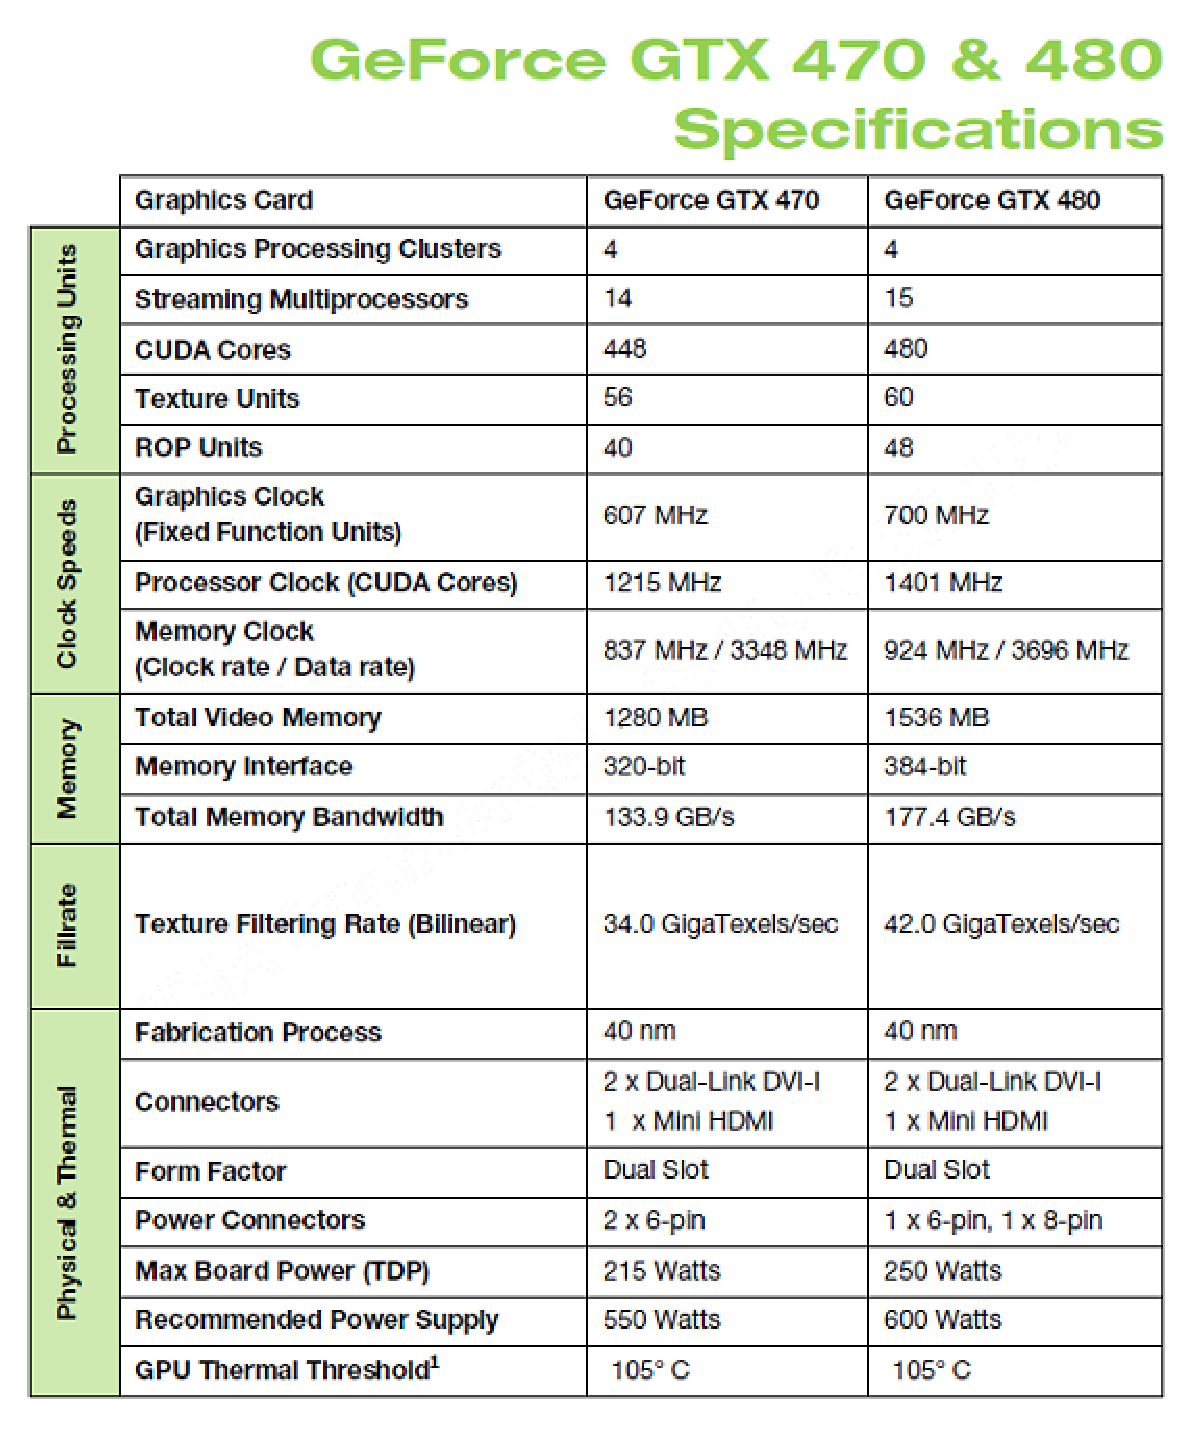
\includegraphics[height=9cm,
    angle=0]{./images/gtx480_470.eps}}
\caption{Comparison GTX 480 vs. GTX 470}
\label{fig:gtx480_470}
\end{figure}

\begin{enumerate}
\item Memory interface\footnote{\url{http://www.techspot.com/review/263-nvidia-geforce-gtx-480/page2.html}}
  \begin{itemize}
  \item Tesla 1st gen: 384-bit = six 64-bit wide memory controllers
  \item Tesla 2nd gen: 512-bit = eight 64-bit wide GDDR3 memory controllers (4GB
  DDR3)
  \item Fermi (GeForce GTX 470): 320-bit = five 64-bit memory
  controllers
  \item GeForce GTX 480: 384-bit = six 64-bit memory partitions $\rightarrow$
    support up to 6GB DDR5, e.g. 3GB DDR5 in C2050, 6GB in C2070. 
  \end{itemize}

\item GPU-CPU memory connection:
  \begin{itemize}
  \item G80: PCI-e Gen1 x16 
  \item G92, GT200: PCI-e Gen2 x16 
  \item GF100: PCI-e Gen2 x16 
  \end{itemize}

\item Clock rate: Different clocks rates are {\it core clock}, a {\it shader
clock} (fast clock)  and a {\it memory clock}. Memory clocks tell how fast the
memory run, i.e. the  memory bandwidth (depending on DDR3, DDR5...).  Depending
on the types of work (shading or general-purpose computing), a streaming
processor (SP) runs at either a higher clock rate ({\bf shader clock}) or a
lower clock rate ({\bf core clock}). In high performance computing, we only use
the concept {\it core clock}.
  \begin{itemize}
  \item G80 has shader clock as 1.35GHz; core clock at 575 MHz,
    memory clock at 999 MHz.
  \item G92 has shader clock as 1.8GHz; core clock at 738 MHz,
    memory clock at 1.1 GHz.
  \item GT200 has shader clock at 1.5GHz, core clock at 648 MHz,
    memory clock at 1.2 GHz.
  \item GT200x2 has shader clock at 1.25GHz, core clock at 576 MHz,
    memory clock at 999 MHz.
  \item Fermi has shader clock at 1.6GHz, core clock
    at 830 MHz (??? 1150 MHz), 
    memory clock at 3.6
    GHz (i.e. 1500 MHz)\footnote{\url{http://www.gigabyte.com/microsite/187/fermi-page.html}}. 
  \end{itemize}

\item Register files (per SM): shared equally by all {\it active} SPs
  in a SM (the concept of ``active'' to be discuss later)
  \begin{itemize}
  \item Tesla 1st gen:  8192 registers of 32-bit (total 32KB). Each
    SP can have 1K entries to be used by 96 threads.

  \item Tesla 2nd gen: 16384 registers of 32-bit (total 64KB,
    i.e. each SM has 16KB, i.e.
    \textcolor{red}{each SP has 2KB register files to be shared by up
      to 128 threads and probably supports 16 or 24 different banks}).
    \textcolor{blue}{Use a single double-precision data consume 2
      register files}.
    The register file is partitioned between thread blocks by the
    JIT/driver. Within the allocation for each thread block, register
    files are statistically assigned to a given thread at
    compile-time. So, we can explicitly tell the maximum number of
    registers to be used by a thread by using the compiler option
    \verb!maxregisters=n!.
    \textcolor{red}{In GT200, an individual thread can have minimum 4,
      maximum 128 registers}.

  \item Fermi: 32768 registers of 32-bit.
    \textcolor{blue}{In Fermi, a thread can have minimum 21 registers
      and maximum 63 registers per threads}

    NOTE:
    \textcolor{blue}{As an SM in Fermi has 4 times SPs compared to an
      SM in Tesla 2nd, the number of register files per thread is half
      compared to that in Tesla 2nd}.
    However, with the availability of L1/L2 cache and shared memory;
    it's hard to justify the performance difference just by looking at
    this.
  \end{itemize}

\item Shared memory:
  \begin{itemize}
  \item Tesla 1: 
  \item Tesla 2: each SM has 16KB shared memory (to be shared by all
    threads in a single block) divided into 16 equally banks. 
  \item Fermi: each SM has 64KB configurable shared memory divided
    into equally 32 banks
  \end{itemize}

\item Two read-only address space: constant vs. texture. 
  \begin{itemize}
  \item Tesla 1
  \item Tesla 2: 64KB constant
  \item Fermi: 
  \end{itemize}

% \item on-chip shared-memory vs. cache: read previous section


\item Special Function Unit (SFU): 
  \begin{itemize}
  \item GT200: each SM has 2 SFU 
  \item GF100: each SM has 4 SFU, i.e. double per SM compared to GT200
  \end{itemize}

\item Floating-point:

  \begin{itemize}
  \item Tesla 1st + 2nd gen: IEEE 754-1985 single-precision for MAD
    (multiply-add) with 128 MAD ops/clock
  \item Tesla 2nd gen: IEEE 754-1985 and increase to 240 MAD
    ops/clock; add support FMAD with 30 FMAD ops/clock,
    i.e. \textcolor{red}{1/8 slower than single-precision}
  \item Fermi: IEEE 754-2008, providing FMA for both single +
    double
    precision\footnote{give more accurate result for an expression}
    with 256 FMAD single-precision ops/clock and 512 FMAD
    double-precision ops/clock.
  \end{itemize}

\item Arithmetic operation for integer:
  \begin{itemize}
  \item Tesla 1st + 2nd gen: hardware support 24-bit; those require
    32-bit run in emulation mode
  \item Fermi: native hardware support 32-bit for all instructions,
    optimized to support 64-bit and extended precision operations
    also.
  \end{itemize}
\begin{figure}[hbt]
  \centerline{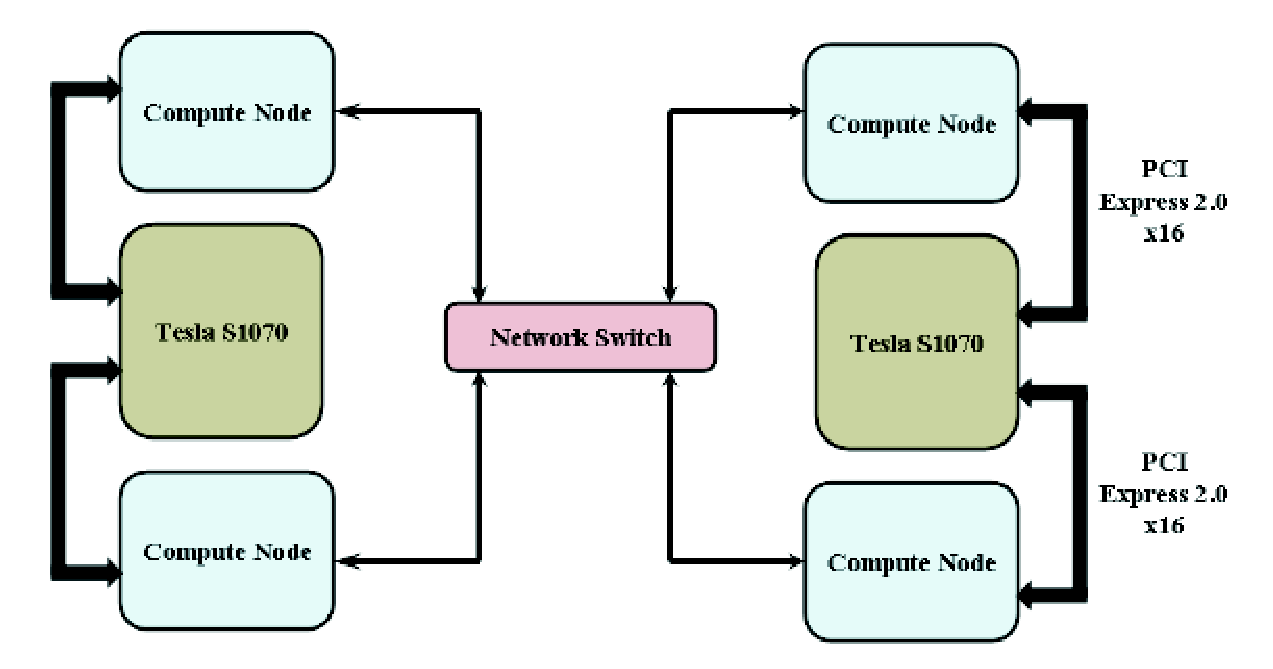
\includegraphics[height=5cm,
    angle=0]{./images/tesla_cluster.eps}}
\caption{GPU cluster: different machines connect via a network switch}
\label{fig:tesla_cluster}
\end{figure}

\item Load/Store (LD/ST) address width
  \begin{itemize}
  \item Tesla 1st + 2nd gen: one load/store unit of 32-bit. It means
    that only one kernel can use GPU at a time. So, if the kernel
    doesn't wide enough to span all cores; that hardware went idle,
    Fig.~\ref{fig:fermi_kernel}(a). 

  \item Fermi: 16 load/store units of 64-bit, i.e. 16 kernels can
    perform load/store data concurrently in a single clock, as shown
    in Fig.~\ref{fig:fermi_kernel}(B) (NOTE: only supports kernels
    from a single program. Kernels from two different programs need to
    run sequentially). However, you need to make sure the kernels are
    independent.  You will learn to create streams and assigning the
    kernel to appropriate stream ID.

  \end{itemize}
  \begin{figure}[hbt]
    \centerline{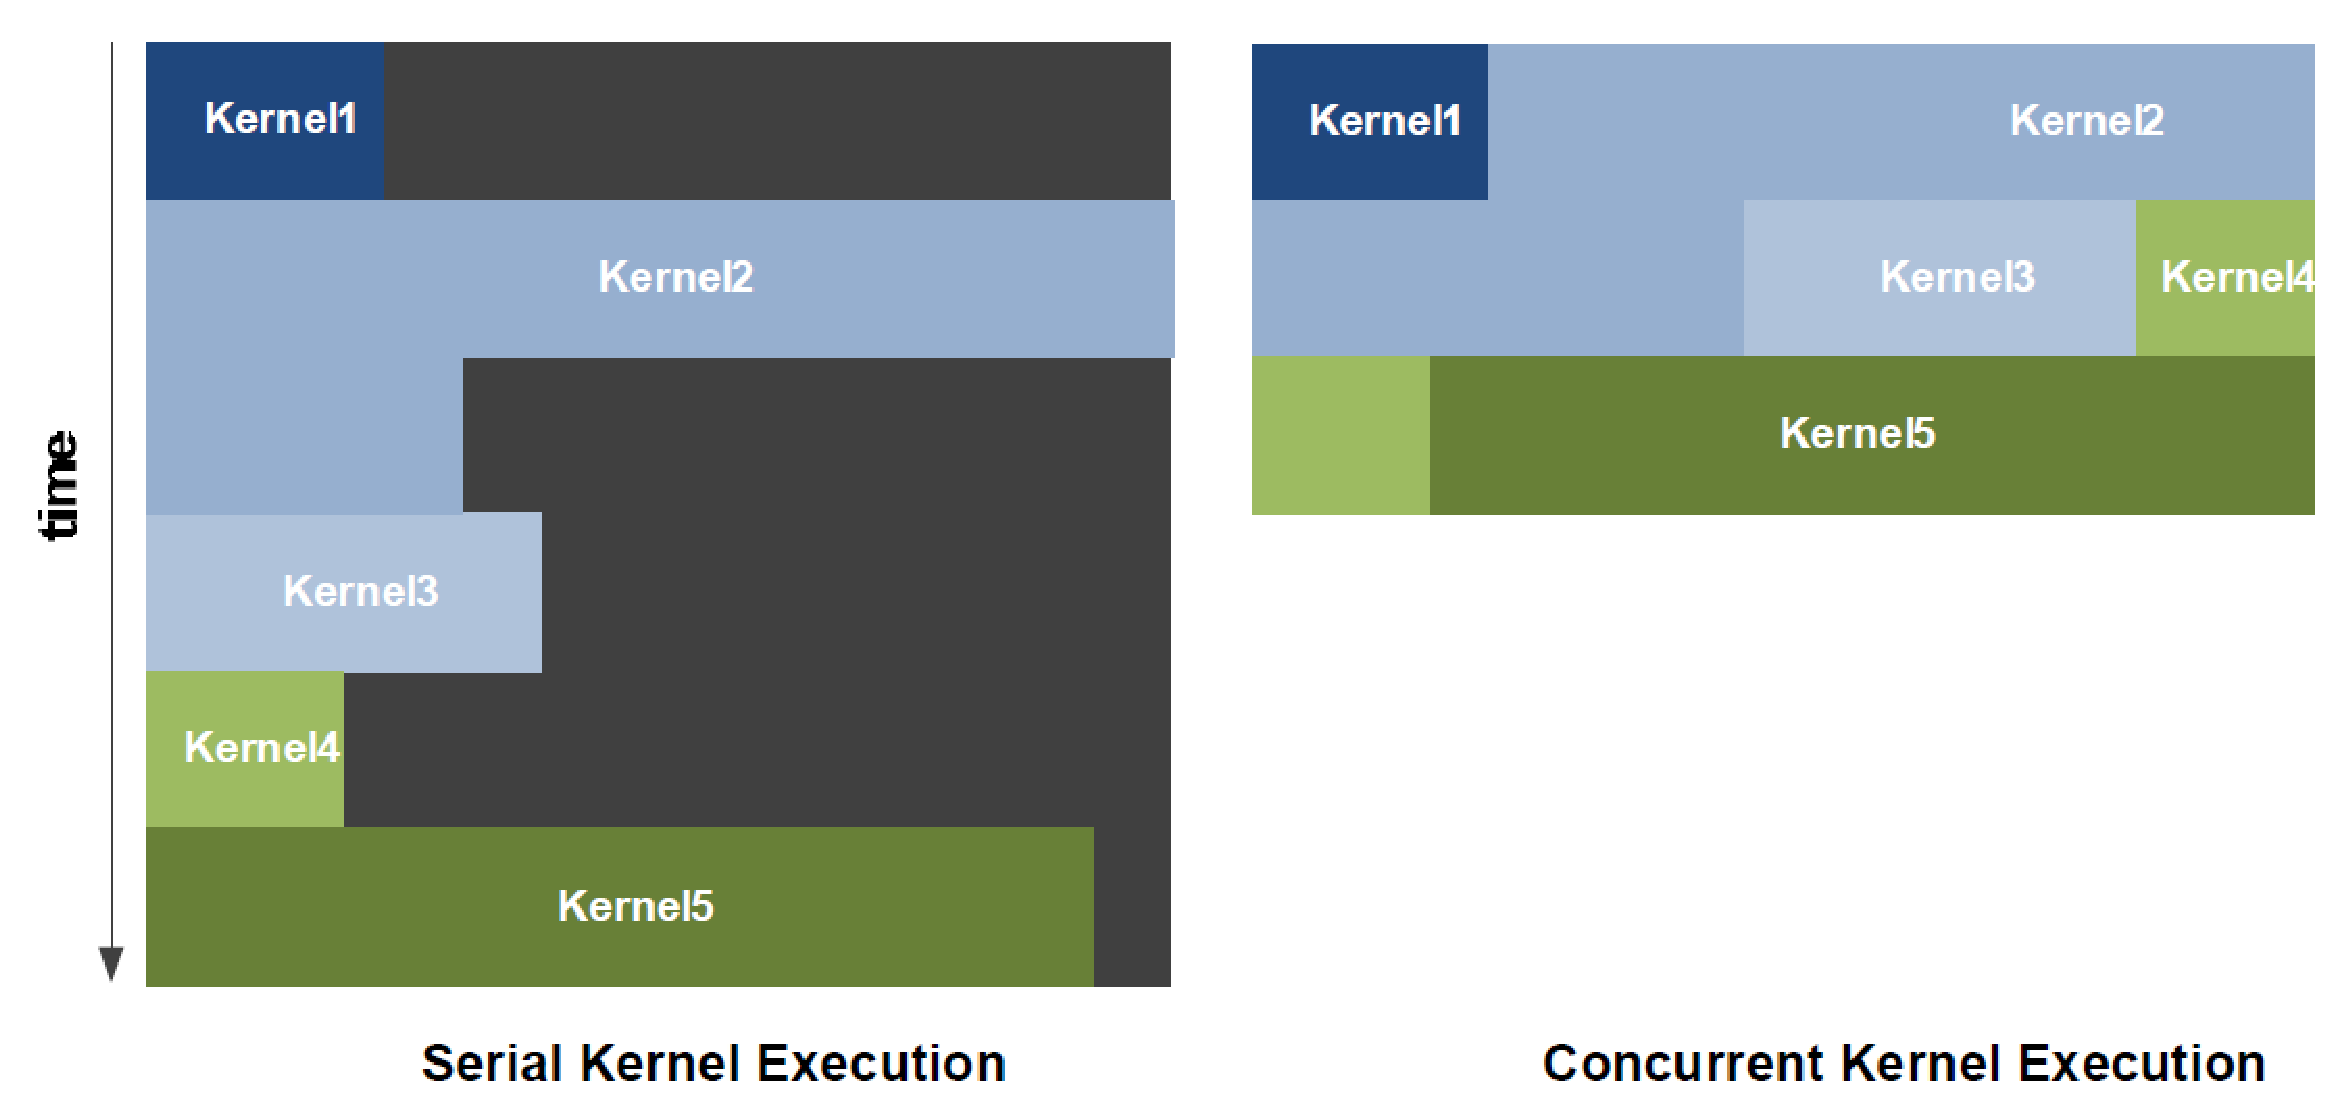
\includegraphics[height=5cm,
      angle=0]{./images/fermi_concurrent_kernel.eps}}
    \caption{(A) sequential kernel execution (B)Fermi concurrent kernels}
    \label{fig:fermi_kernel}
  \end{figure}

\item Context switching (each program receives a time slice of
  processor's resource)
  \begin{itemize}
  \item Tesla 1st + 2nd gen: 250 microseconds
  \item Fermi: below 25 microseconds (10x faster), concurrent
    kernel execution, better kernel-to-kernel communication
  \end{itemize}

\item Warp scheduler:
  \begin{itemize}
  \item Tesla 1st + 2nd gen: single warp scheduler $\rightarrow$ only
    a single kernel can run on GPU

  \item Fermi: two warp schedulers, with faster context switching,
    $\rightarrow$ allows more threads to be able to run in parallels,
    improved thread block scheduling.
  \end{itemize}

\end{enumerate}

 
\subsection{Fermi Streaming Multiprocessor (SM)}
\label{sec:fermi-sm}

Tesla GT200 has 8 CUDA core per SM. Each SM in Fermi, with 32 CUDA cores, can
handle 48 warps simultaneously. The CUDA core, again is a unified processor core
that can execute vertex, pixel, geometry, and compute kernels.

In Fermi, each streaming multiprocessors (SM) is composed of
\begin{enumerate}
\item a CU (control unit): decode/encode instructions, and schedule threads
\item a pipeline for execution: int, fp32, fp64, special-functions...
\item 32K of 32-bit registers (large, but potentially divided by
  thousands of threads; so number of registers per thread is
  limited). Each thread can have maximum 63 registers, and minimum 21
  (if threads fully populated).
\item shared memory (with register speed, but accessible to different
  threads) = a programmer-managed scratch-pad memory
\item L1 data cache, and constant cache: hardware-managed caches
\item texture unit : also hardware-managed cache, but is read-only and
  widely used for graphical application
\end{enumerate}

Each SM can allow maximum 1536 concurrent threads. 

Expectation:
\begin{enumerate}
 \item Fermi M2090: has 512 cores that can deliver 665 GFLOPs of peak
  double-processing performance. NOTE: Amber use four M2090 + one CPU can run
  69 nanosecond simulation in one day. The fastest performance on CPU for AMBER
  can deliver 46 ns/day. M2090 is equipped on server machine, not workstation
  \footnote{\url{http://pressroom.nvidia.com/easyir/customrel.do?easyirid=A0D622CE9F579F09&version=live&prid=757066&releasejsp=release_157&xhtml=true}}.
 
 \item Kepler C3070 can deliver 1.425 TFLOPs in double-precision, about 2.7
 times faster than C2050. 
 
 \item Maxwell C4070 can deliver 3.925 TFLOPs in double-precision, about 7.6
 times faster than Fermi C2070. 
\end{enumerate}

\begin{enumerate}
  \item 16 LD/ST units per SM: allowing source and destination address to be
  calculated for 16 threads per clock. Address can be in cache or global memory.
  
\item It supports up to 1536 concurrent threads
\item It has 32K 32-bit registers with \textcolor{red}{up to 63
    registers per thread} (21 if threads fully populated)

\item 4 SFU units: to execute transcendental functions (sin, cosine, reciprocal, and
square root). Each unit can execute one instruction per thread per clock. So a
warp of 32 threads take \textcolor{red}{8 clocks} to complete one transcendental
function.

\item Instruction throughput
  \begin{itemize}
  \item 2 fp32 pipes, each: 1 warp (or 32 threads) per 2 clock cycles
  \item 2 int32 pipes, each: 1 warp per 2 clock cycles
  \item 1 fp64: 1 warp per 4 clock cycles
  \item 1 SFU : 1 warp per 16 clock cycles (when using transcendental
    functions) 
  \end{itemize}

\item 64K total SMEM/L1 cache which can be partitioned into 16KB/48KB or
  48KB/16KB. The data in L1-cache can be shared between threads in the same SM
  (i.e. threads from the same grid block); but not across SM. Otherwise, we need
  to use L2-cache.

\begin{framed}

   We use more SMEM (48/16 configuration) to improve memory access for
   algorithms with well-defined memory access. Otherwise, L1 cache (16/48
   configuration) can be used to improve memory access for irregular algorithms
   where data addresses are not known beforehand.
   
   For graphics program, GF100 uses 48/16 configuration, where 16KB L1 cache
   acts as a buffer for register spills.
\end{framed} 

\item Shared memory (SMEM) is organized into 32 banks, each with
  32-bit wide. Now, support multicasting (previously only support
  broadcast). 

\item Coherent L2 cache with 128KB per memory controller, i.e. 768 KB
  in total. NOTE: AMD Cypress has 512 KB of L2. 

\item There is no native \verb!int64! instructions (integer
  arithmetic). However, there is magic to minimize needed \verb!int32!
  instructions. 
\end{enumerate}


\subsection{Graphic Enhancement}
\label{sec:Fermi_graphics-enhancement}

GF100 doubles the number of CUDA per SM (32 from 8). The geometry pipeline has
better geometry shading, stream out, and culling. GPC in GF100 features two
important innovations: (1) scalable Raster Engine for triangle setup,
rasterization, and Z-cull, and (2) a scalable PolyMorph Engine for vertex
attribute fetch and tessellation.

ROP units per ROP partition is doubled and fillrate is greatly improved. GF100
has 48 ROP units for pixel blending, antialiasing, and atomic memory operations.
The ROP units are organized in six groups of eight. Each group is serviced by a
64-bit memory controller

8xMSAA peformance is improved through enhanced ROP compression.

NOTE: The most advanced games use 1-2 milliions polygons per frame. In
computer-generated films, they use hundreds of millions of polygons. This is a
challenge to GPU, as the number of pixel shaders increased (from one to many
hundreds), but the triangle setup engine is still a singular unit. The two below
techniques are mostly used in films to create the intimately detailed
characters: tessellation + displacement mapping.
\begin{itemize}
  \item Tessellation: refines large triangles into a collection of small
  triangles
  \item Displacement mapping: change their relative position
\end{itemize}
GF100 can deliver high performance in tessellation and geometry throughput that
allows gaming applications to utilize the two techniques. Tessellation is
enhanced by the introducing of PolyMorph Engines (discussed below).

\begin{framed}
Objects and Characters in Games can be created using Software Modeling Packages:
MudBox, ZBrush, 3D Studio Max, Maya, SoftImage. The models are meshed of
triangles with associated texture maps need for proepr shading. In games, the
model information is sent per frame to the GPU through the Host Interface. 

Due to the limited bandwitdh of PCI-e bus, game developers tend to use
relatively simple geometric models. With the Tessellation unit on GPU, game
developers need to send a compact geometric representation of the
object/character, and the GPU can produce the correct geometric complexity for
the specific scene, Fig.\ref{fig:Ex_Tessellation}.
\end{framed}

\begin{figure}[hbt]
  \centerline{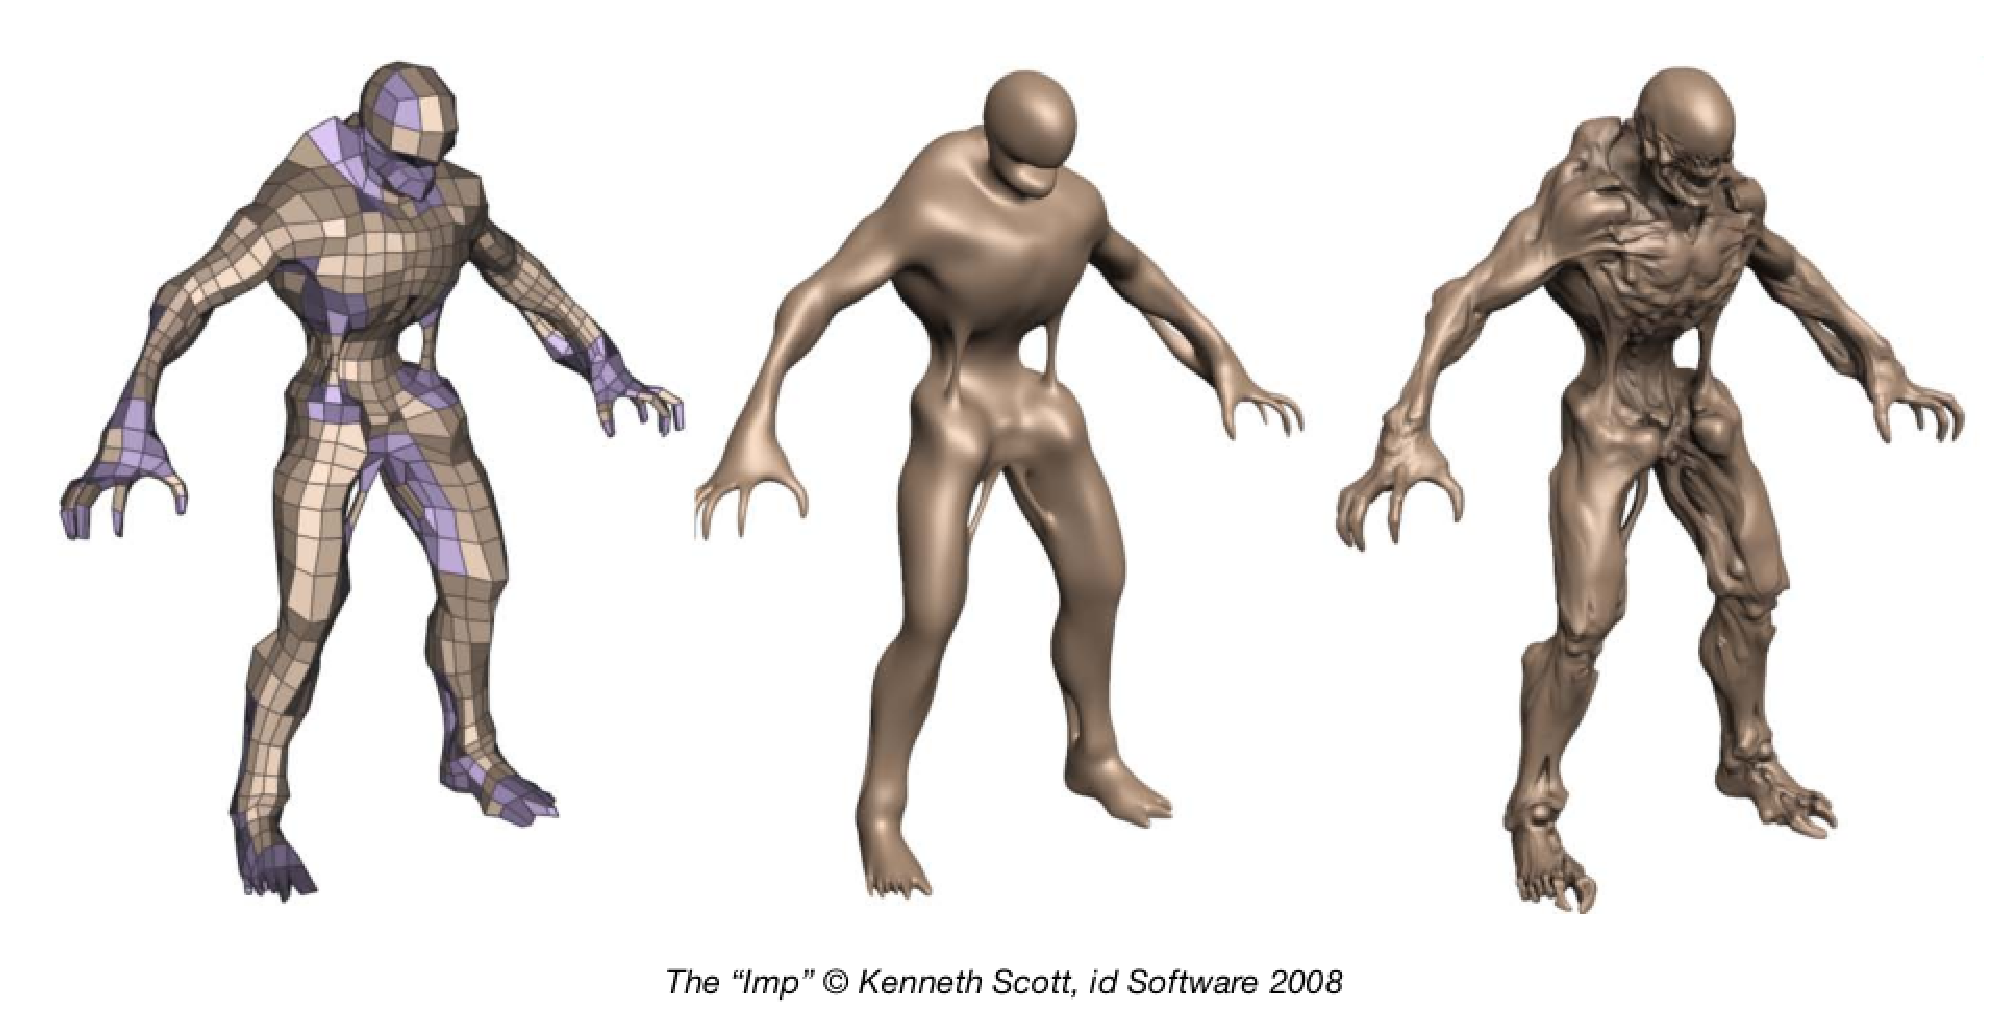
\includegraphics[height=5cm,
    angle=0]{./images/Ex_Tessellation.eps}}
  \caption{(A) A compact representation (quad mesh); (B) After Tessellation;
  (C) Tessellation first then applying Displacement Map}
  \label{fig:Ex_Tessellation}
\end{figure}


The traditional geometry processing architecture at the front-end of the
graphics pipeline is replaced by using multiple ``PolyMorph Engines''. Fermi
GF100 has 16 PolyMortph Engines. With tessellation, the triangle density
increases by multiple orders of magnitude. To rebalance the graphics pipeline to
handle high triangle rates, a scalable geometry called PolyMorph Engine is
developed (Sect.\ref{sec:polymorph-unit-+}).

On-chip L1 and L2 cache enables high bandwidth transfer of primitive attributes
between SM and the Tessellation Unit, and between different SMs. Tessellation
and all of its supporting stages can be done in parallel.

\subsection{Compute Enhancement}

GF100 has faster context-switching between graphics and PhysX (using GigaThread
Engine), concurrent kernel execution, and enhanced caching architecture (good
for irregular data access such as Ray Tracing).

GF100 has better atomic operations. GF100 implements IEEE 754-2008
floating-point standard, with FMA instruction for both single and double
precision. The newly designed integer ALU supports full 32-bit precision for all
instruction (i.e. native 32-bit integer arithmetic). Also, the integer ALU is
optimized to support 64-bit and extended precision operations. Double-precision
is now half-speed compared to single-precision.

New intrinsic operations: boolean, shift, move, compare, convert, bitfield
extract, bit-reverse insert and population count.

\section{Unified Virtual Address (UVA): from Fermi (CC 2.0) with CUDA 4.0}
\label{sec:UVA}
\label{sec:cuda4_UVA}


The NVIDIA Fermi GPU architecture, introduced in 2009, implemented a unified GPU
address space spanning the three main GPU memory spaces (thread private local
memory, thread block shared memory, and global memory) which was applied to
GPU-side data only (Sect.\ref{sec:SM-Fermi}).

In 2011, CUDA 4 introduced Unified Virtual Addressing (UVA) to provide a single
virtual memory address space for both CPU and GPU memory and enable pointers to
be accessed from GPU code no matter where in the system they reside, whether in
GPU memory (on the same or a different GPU), CPU memory, or on-chip shared
memory

The Fermi architecture support PTX ISA version 2.0, i.e. CC 2.0
(Sect.\ref{sec:CC2.0}).
PTX ISA 2.0 support unified virtual address space (UVA),
Fig.\ref{fig:Fermi-unified-address-space}, which is provided via CUDA 4.0 via 
the new API \verb!cudaHostAlloc! (Sect.\ref{sec:cudaHostAlloc}).

\begin{mdframed}

Previously, CUDA treats pointer to host-memory and pointer to device-memory differently.
Kernels can only uses pointers to device-memory (Sect.\ref{sec:GPU-pointer-pre-Fermi}).
Because of that, explicit calls to CUDA APIs to transfer data back and forth are required
\begin{verbatim}
cudaMemcpyHostToHost
cudaMemcpyHostToDevice
cudaMemcpyDeviceToHost
cudaMemcpyDeviceToDevice
\end{verbatim}
\end{mdframed}

UVA provides a single virtual memory address space, and the physical memory
where data resides is in fact on CPU side, i.e.  using the host memory from the
special memory region called th

In order to achieve UVA, the data is allocated on pinned CPU memory (pinned host
memory) or page-locked memory (Sect.\ref{sec:page-locked-memory}). This is
achieved by calling
\begin{verbatim}

\end{verbatim}

The pointer variable, pointing to data on page-locked memory, can be used on
GPU-side via PCI-e bus. This enables a single pointer, that is used for
accessing data from either GPU code or CPU code.

% , no matter where in the system they reside, whether its device memory (on the
% same or a different GPU), host memory, or on-chip shared memory.
\begin{itemize}

  \item The benefit is that data always reside on CPU-side. UVA does not
  automatically migrate data from one physical location to another, like Unified
  Memory does.

  Because of that, we say {\bf UVA enables “Zero-Copy” memory}, i.e. kernel code
  access the pinned host memory over PCI-Express, i.e. no 2 pointers mechanism
  is needed which always requires an explicit memcpy, and no implicit copy is
  done never.
  
Indeed, if zero-copy provided a degree of convenience in relation to data access
operations, UVA took this one step further by improving on data transfer tasks.

Zero-Copy provides some of the convenience of Unified Memory introduced in CUDA
6.0 (Sect.\ref{sec:Unified-Memory-CUDA6.0}), i.e. free users from managing the
explicit copy, but none of the performance, because it is always accessed with
PCI-Express’s low bandwidth and high latency.
  
\end{itemize}

The true benefit of the UVA mechanism becomes apparent when transferring data
between two devices. When all devices plus the host shared the same virtual
address space, a data access or data transfer involving two devices was
simplified in two respects:
\begin{enumerate}
  \item  Straight use on device A of a pointer to access memory on device B,

  \item  No need for staging the data transfer through host memory.
  
  Data can be transfered directly from GPU-1 memory to another GPU-2 memory,
  without having to copy first into the (intermediate) host memory.
  
  Here: data movement between GPUs through peer-to-peer transfers -
  Sect.\ref{sec:cudaMemcpyPeer}
  
\end{enumerate}
\url{https://www.nvidia.com/docs/IO/116711/sc11-multi-gpu.pdf}

CUDA 6.0 provides the TRUE unified memory - Sect.\ref{sec:Unified-Memory-CUDA6.0}.

Now, with unified memory and universal virtual addressing (UVA), one function
can handle all \verb!cudaMemcpyDefault!. As the virtual memory space used by UVA
is 40-bit memory space, the system need to be 64-bit. Data location becomes an
implementation detail, and it frees the programmer from handling this.

\begin{figure}[hbt]
  \centerline{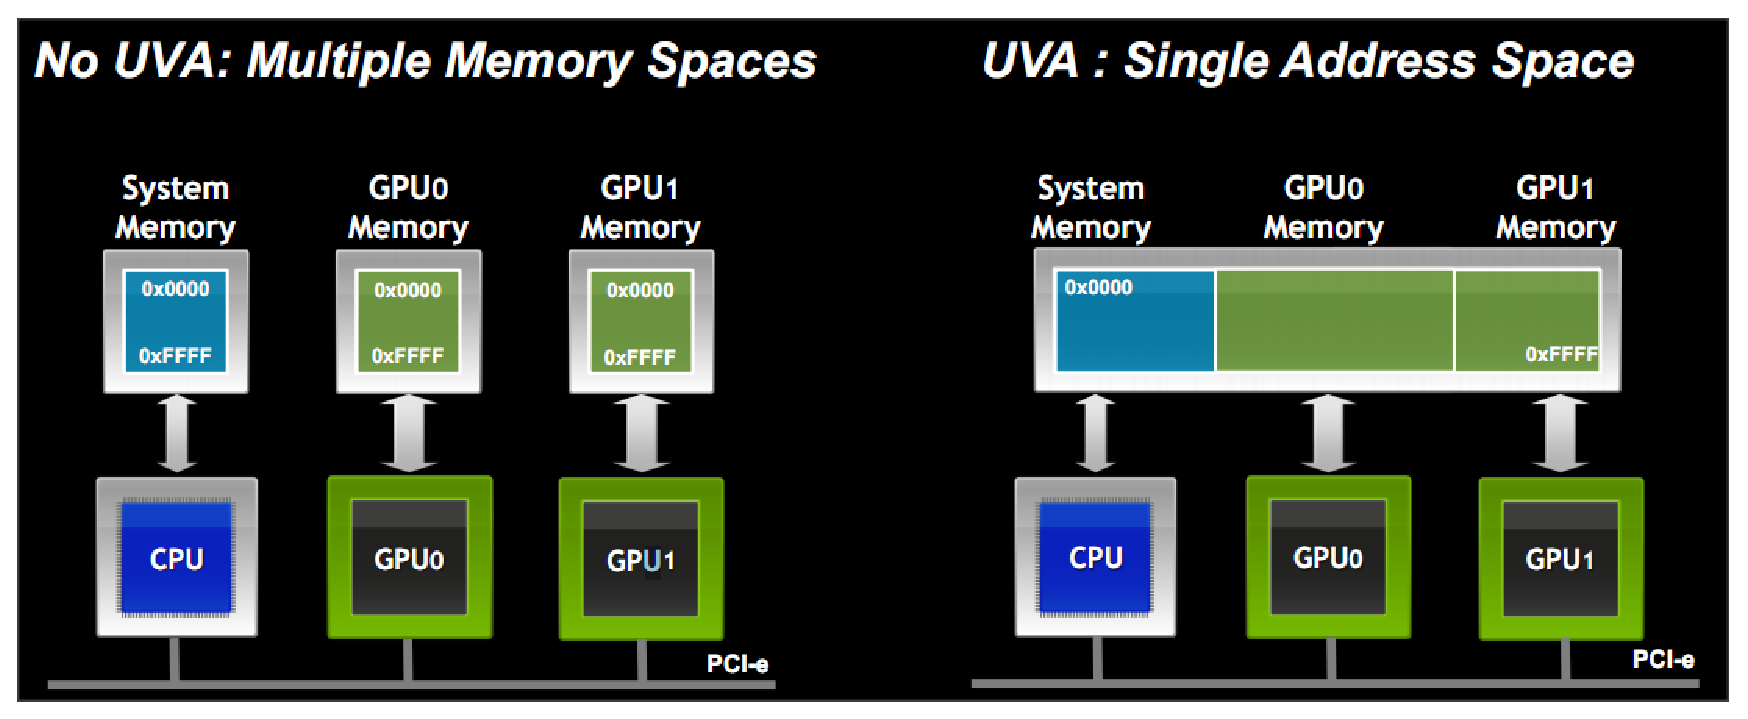
\includegraphics[height=5cm,
    angle=0]{./images/UVA_CUDA4.eps}}
\caption{UVA on Fermi-based GPU with CUDA 4.0}
\label{fig:fermi_UVA}
\end{figure}

In addition, same assembly instruction can be used for gmem,
smem... In addition, it enables function calling on GPU. % The space is
% 32-bit or 64-bit addresses with the default is based on the O.S. 
The space is still 40-bit, as with GT200. However, now local, shared
and global memory shared the same address space. So, you can use
pointers to point to data in any of those memories. 

\begin{figure}[hbt]
  \centerline{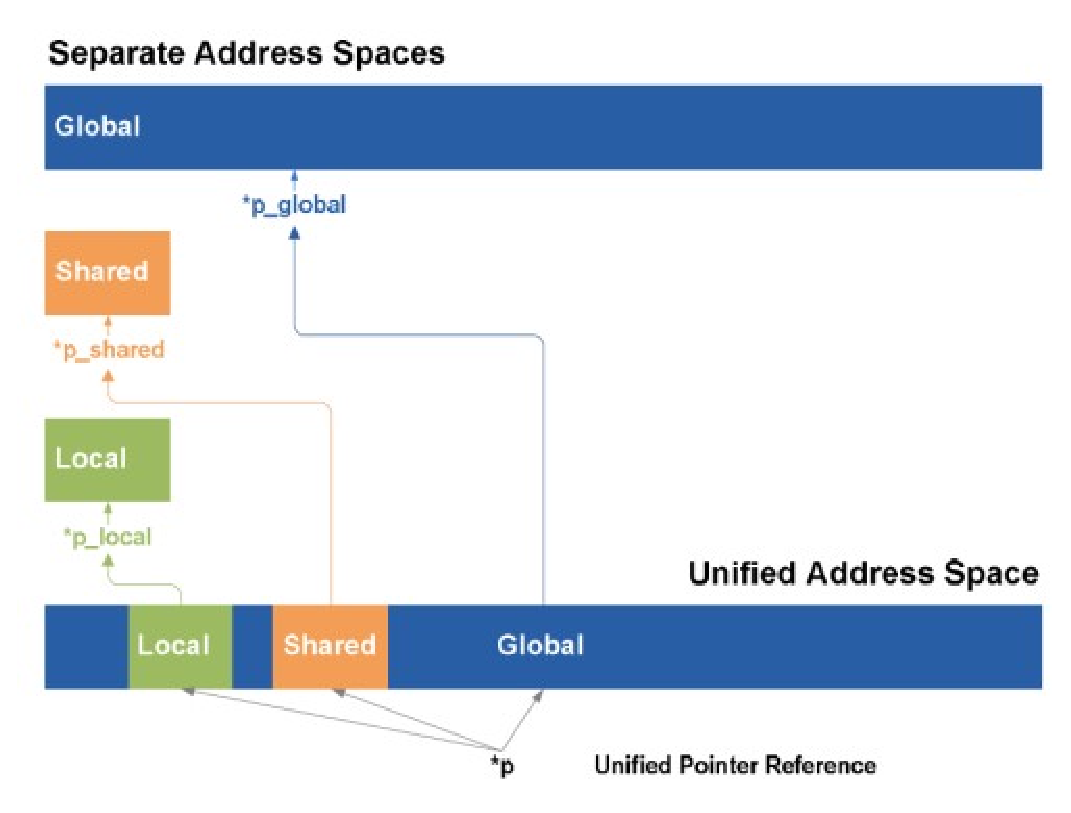
\includegraphics[height=5cm,
    angle=0]{./images/unified_memory.eps}}
\caption{Unified Memory pointers}
\label{fig:unified_memory}
\end{figure}

Using Direct Memory Access (DMA) on PCI-e Gen2, UVA allows
(Sect.\ref{sec:GPUs_share-data}:
\begin{enumerate}
  \item Direct Access
  \item Direct Transfer: Copy GPU A-GPU B without going through host memory
  (see requirements)
\end{enumerate}
Saturated bandwidth is $>$ 6GB/sec, and low latency: 1 PCI-e transaction + 1
memory fetch (about 2.5ns).

\textcolor{red}{CONS of UVA (compared to Unified Memory in CUDA 6.0+ and CC3.0+)}:
A device thread has to reach out to get the data. No guarantee of coherence is
provided as, for instance, the host could change the content of the pinned
memory while the device reads its content

   
\subsection{Physical and Virtual address space}
\label{sec:phys-virt-memory}

In early designs of Tesla architecture, it doesn't have virtual memory design,
only one kernel of a single program can use the GPU at a time. Now, Fermi
architecture supports CPU-style virtual memory architecture with 64-bit address
line, and physical memory with 40-bit address line (support up to 1TB of device
memory). This allows multiple kernels from a single program can run
simultaneously, i.e. each kernel use its own virtual address space, which then
can be mapped to the physical address by the GPU.

Even though kernel and host functions share the same virtual address space;
currently, kernel function cannot access host memory, and vice versa. So, all
data must be copied to GPU before passing it to the kernel; and all result must
be copied back to the host memory before passing it to a host subprogram.

\begin{figure}[hbt]
  \centerline{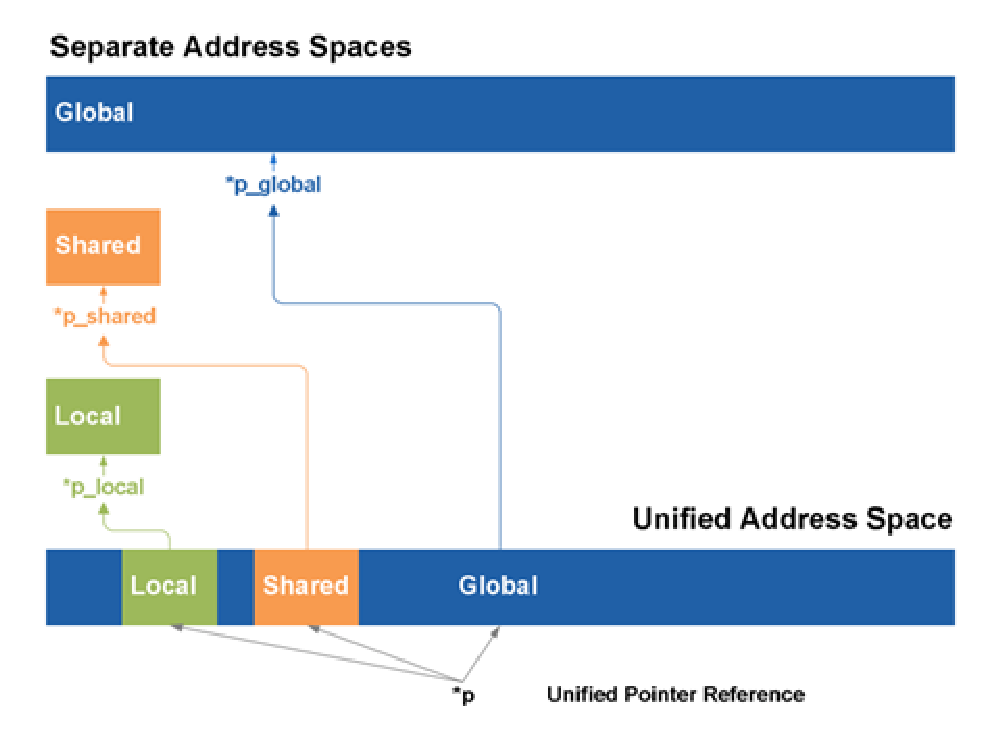
\includegraphics[height=6cm,
    angle=0]{./images/Fermi_unified-address-space.eps}}
  \caption{Fermi with CUDA 4.0+ using PTX 2.0 ISA share space with CPU}
  \label{fig:Fermi-unified-address-space}
\end{figure}


To check if the device supports unified addressing, we do
\begin{verbatim}
cudaPointerAttributes prop;
errorCode = cudaGetDeviceProperties  (prop, devID);

if (prop.unifiedAddressing == 1) then "Support"   
\end{verbatim}
NOTE: All devices with CC 2.0 and above running on 64-bit processes have unified
addressing enabled automatically. 

\begin{framed}
On Windows 7 and Vista, TCC driver model need to be used to enable unified
addressing. 
\end{framed}
 
\subsection{Data copy host $\leftrightarrow$ device, and device A
$\leftrightarrow$ device A}

Since this virtual memory share the same address space with CPU RAM, it's
impossible to tell if a pointer is pointing to a memory on CPU or GPU. This free
CUDA programmers from telling the CUDA driver APIs the direction of the data
transfer. So, to copy data from one location to another, we still use
\verb!cudaMemCpy()! yet we don't need to specify the direction.
Instead, we only use \verb!cudaMemcpyDefault! option.

\begin{verbatim}
errorCode = cudaMemcpy  ((void**) dst, (void**) src, numBytes,
        cudaMemcpyDefault);
        
cudaMemcpy(gpu0_buf, host_buf, buf_size, cudaMemcpyDefault)
cudaMemcpy(gpu1_buf, host_buf, buf_size, cudaMemcpyDefault)
cudaMemcpy(host_buf, gpu0_buf, buf_size, cudaMemcpyDefault)
cudaMemcpy(host_buf, gpu1_buf, buf_size, cudaMemcpyDefault)
\end{verbatim}

\begin{figure}[hbt]
  \centerline{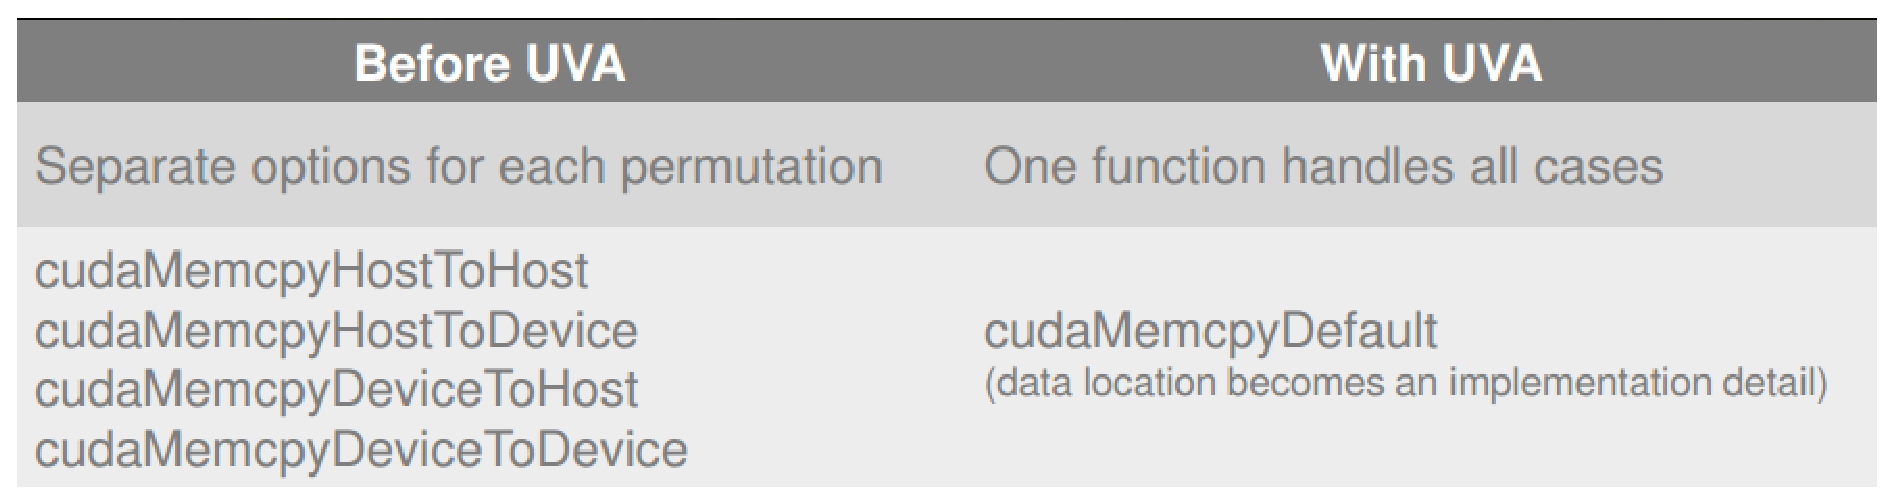
\includegraphics[height=3cm,
    angle=0]{./images/Fermi_UVA.eps}}
  \caption{UVA Fermi}
  \label{fig:Fermi_UVA}
\end{figure}

 
\subsection{Data copy device A $\leftrightarrow$ device B}

In 64-bit systems, if there is more than one devices on the system, they are
share the same virtual addressing space. As a result, CUDA 4.0+ support copy
data from one GPU to another GPU via DMA (direct memory access). This is known
as {\bf peer-to-peer memory copy}. This feature is used in GPUDirect technology
that allows using multiple-GPU (Sect.\ref{sec:multi-GPU_CUDA4.0}).

\begin{verbatim}
cudaMemcpy(gpu0_buf, gpu1_buf, buf_size, cudaMemcpyDefault) 
\end{verbatim}

Requirements:
\begin{enumerate}
  \item 2 GPUs on the same IOH
  \item Nvidia driver v270.41.19 or later
  \item CUDA 4.0+
  \item Fermi-class GPU
  \item 64-bit system
  \item Linux, or Windows with TCC driver.
\end{enumerate}

\section{Data and memory access}
\label{sec:data-memory-access}


\begin{enumerate}
\item Shared memory (SMEM) is programmer-managed scratch-pad memory

\item L1 data cache, constant cache: Hardware-managed caches

\item Texture unit: Hardware-managed cache for textures,
  interpolation/conversion unit
\end{enumerate}

\begin{figure}[hbt]
  \centerline{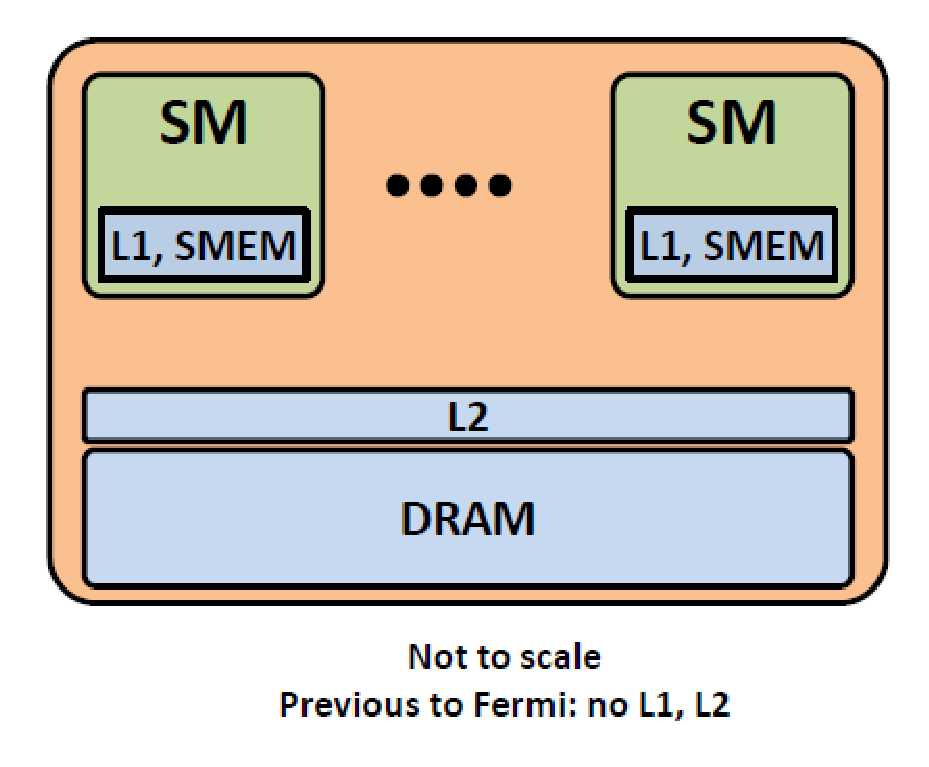
\includegraphics[height=5cm,
    angle=0]{./images/Fermi.eps}}
\caption{Fermi in brief}
\label{fig:Fermi}
\end{figure}

2D/3D thread blocks should be a multiple of 32 ``wide''. Data should
also be a multiple of 32 in the fastest-varying dimension. 


\section{Roles of constant memory and texture in Fermi???}
\label{sec:roles-const-text}

{\bf Questions: should we use texture cache or constant memory or L1
  and/or L2 cache?}

\begin{enumerate}
\item At first, and the most important, we only consider using texture
  cache or constant memory if the data is read-only.

\item Using constant memory is fast when the data is cached in the cache memory
and if all threads in the same half-warp read the same memory address
(Sect.\ref{sec:constant-memory}. Otherwise, sequential reads occur to these data
in the constant-cache memory.

\item Random load from texture could be a lot faster, than random load load from
  global memory. FERMI L1 cache to L2 datapath is 128 bytes wide, so
  with random access you could not use all L1 to L2(and memory)
  bandwidth. FERMI L1 texture cache to L2 datapath is 32 bytes wide
  (my guess!) , so random load is not a problem.

  i.e. Fermi L1 cache line size is 128 byte. If threads inside warp
  access different cache lines, EVEN if they all is inside L1 cache,
  your got 1/32 L1 theoretical bandwidth, because each thread issues
  one 128 byte transaction to get 4 byte float value.  Texture cache
  and shared memory don't have such problem.

\item Global memory accesses also could be 32 bytes wide, if they
  bypass L1 cache at all(compiler switch). With texture cache you get
  both: and L1, and small load granularity.
\end{enumerate}

\begin{framed}
  The cache line is the minimum amount of data that a single thread
  retrieve from memory (e.g. 128 bytes), regardless of how many data
  it truly needs (e.g. 32 or 64 bytes). So, 
  \begin{itemize}
  \item if threads read 4-byte data in the same cache lines, we only
    need a single memory read
  \item if threads read 4-byte data, each element in a separate cache
    lines (though all data elements are residing in the L1 cache), we
    still need individual memory read for a single thread, which means
    we only use 1/32 theoretical bandwidth; and that slow down the
    performance 
  \end{itemize}

  As texture cache has the cache line is 32-bytes, then if a single
  thread read in float4 data, i.e. 8-byte, the penalty is 1/4; rather
  than 1/32. 
\end{framed}

I think using texture still have many benefits in accessing data
located in CUDAArray (optimize for 2D and 3D).

its probably dependant on the access pattern.  I saw 20-30\%
degragation going from textures to gmem (i.e. textures were faster),
even with L1, with the following access pattern.
\begin{lstlisting}
float fValue = tex1DFetch( tex1, iIndex ) * w1 + 
     tex1DFetch( tex1, iIndex + 1 );  //or get a float2 out of the
                      //textures.... 

\end{lstlisting}
For me L1 seems just to make things worse (increasing L1 to 48K and
reducing Shared mem to 16K also reduced occupancy and resulted in
slower performance) - I guess it was mostly usefull for register
spilling enabling me to use the -maxrregcount and thus increase
occupancy by moving spilled registers to the L1.


I asked Michael Garland about textures vs. L1 in his presentation for
at the VSCSE summer school last week. He confirmed what we are saying
here, that sometimes L1 is better and sometimes the tex cache was
better for the sparse matrix vector multiply kernels he works on. The
interesting thing he added is this:
\textcolor{red}{added benefits are possible by making use of both
  caches in a single kernel}.
They are independent caches, after all!
\textcolor{red}{The idea is to read from one array with tex1Dfetch (or
  tex2D/3D) and from the others with L1}.
1) It limits the L1 cache pollution and 2) It gives you a larger
amount of cache memory to read from.

I've only got one kernel that performs cached reads from 2 different
arrays which I can try this idea out on - it did lead to a slight
performance improvement. The improvement likely wasn't that great
because the 2nd array read is not in the inner loop and only performed
once for every ~30-40 inner loop random reads.

It is too bad that the tex cache is so shrouded in secrecy that we
can't know what access patterns work well for it. Even a cache line
size would be something! 

Many people experience a drop in performance when trying to use 64KB
L1
cache\footnote{\url{http://forums.nvidia.com/index.php?showtopic=167561}}.
It's better to use L2 cache only (i.e. use \verb!-dlcm=cg! compiler
option). 

Shared memory doesn't have cache lines at all.

There's a big difference between cache lines and banks. Cache lines
are groups of 128 contiguous bytes aligned to 128 byte
boundaries. GF100 copies values from device memory to L2 and from L2
to L1 in these 128 byte chunks.

Banks are unrelated to cache lines. GF100 shared/L1 has 32 banks, each
corresponding to the low order words of the address. At each
instruction tick, each bank can output its 4-byte-word to one thread
who requests a word with that low order address. If two threads
request different memory with the same low order word addresses, the
bank can only service one of them, and another instruction tick is
needed to service the next.. they're serialized. (There's an exception
for a single word broadcast of the identical address though.)

Your quote from the programming manual discusses a different topic,
multi-word accesses by threads. L1 behaves just like shared memory in
this case, with identical inevitable bank conflicts.

\begin{framed}
  I think it's clear now that threads of the same warp in my program
  are accessing different cache lines of L1 cache that make it worse
  than texture cache. L1 cache is accessed in the unit of 128-bit
  cache lines. And what about texture cache? How was it accessed?
\end{framed}

In GT200, constant memory access is recommended to use known offset
(for ...) and threadIdx.x as offset (for ...). In Fermi, constant
memory access with known offset is essentially free.  In addition,
Fermi is RISC processor, with instruction arguments come from
registers, immediate constants or constant buffer. Otherwise, separate
load instruction is needed

There are two cases of constant memory
\begin{enumerate}
\item the constant data is literal, i.e. part of the instruction
  itself, e.g. 3.1415
\begin{lstlisting}
mul.f32 r0 r1 3.1415
\end{lstlisting}

\item the constant data need to be loaded from constant memory
\begin{lstlisting}
mul.f32 r0 r1 c0[10]
\end{lstlisting}
  The data from c0[10] is loaded into the register r1. However, we
  don't need a separate memory load instruction

\end{enumerate}

Example: to add value from constant memory you need only one
instruction
\begin{lstlisting}
add.f32 r0 r0 c2[0x35]
\end{lstlisting}

Example: to add value from global memory you need a load and an add
\begin{lstlisting}
ld.u32 r1 g[0x35]
add r0 r0 r1
\end{lstlisting}

\begin{lstlisting}
#immediate constant
set $p0 ne u32 $r4 -0x1

#constant buffer
add b32 $r12 shl $r13 0x2 c2[0xc8]

#global memory
ld b32 $r4 ca g[$r12(null)+0]

#constant buffer with unknown offset
ld b32 $r17 c2[$r17(null)+0x20]
\end{lstlisting}

Constant memory:
\begin{enumerate}
\item a bit faster than from global memory
\item doesn't require separate load instruction
\end{enumerate}

Texture load is faster than normal global memory. Global memory load
granularity is 128 bytes. It means that if you only need 4 bytes, the
hardware also fetches 124 neighboring bytes too. Texture load
granularity is 128 bytes at L1 level and 32 bytes at L2 level. So,
depending on compiling setting, you can determine which one to use. 

Fermi L1 cache line size is 128 byte. If threads inside warp access
different cache lines, EVEN if they all is inside L1 cache, your got
1/32 L1 theoretical bandwidth, because each thread issues one 128 byte
transaction to get 4 byte float value.  Texture cache cache line is
32-byte so float can be accessed alone by individual threads.  Thus
texture cache and shared memory don't have such problem.

A cache line in L1 or L2 is 128 bytes and maps to a 128-byte aligned
segment in device memory.  If the size of the words accessed by each
thread is more than 4 bytes, a memory request by a warp is first split
into separate 128-byte memory requests that are issued independently.
Each memory request is then broken down into cache line requests that
are issued independently. A cache line request is serviced at the
throughput of L1 or L2 cache in case of a cache hit, or at the
throughput of device memory, otherwise.


Texture:
\begin{enumerate}
\item random load from texture is a lot faster than load from global
  memory 

\item Fermi 12KB L1 texture cache (per 4 texture units) and L2 datapath is
32-byte wide, so random is not a problem. A random access means non-regular and is
  defined as (1) random or unknown at runtime, or (2) access pattern
  is non-linear (neither is it square or cubic)
\begin{lstlisting}
int offset = random()%SIZE;
int value = array[offset];
\end{lstlisting}
  The speedup of texture memory (besides free interpolation from 2D/3D
  to 1D) is when you access it linearly or in a blockwise fashion
  (2-d). if you're storing to shared memory you can definitely read it
  in linearly. maybe in each block read in (x-2,y-2) to (x+w+2,y+h+2)
  and then run the filter in parallel from (x,y) to (x+w,y+h).

  an advantage of this is that varying your filter size will have a
  fairly neglible effect on your i/o utilization. and it's deliberate
  and exact instead of cacheing which is more heuristic and might make
  the wrong decisions.


\item As Fermi L1 and L2 cache is to 128-byte wide, with random
  access, we doesn't utilize all L1 and L2 memory bandwidth. In other
  words, texture is a better choice for non-sequential or random
  memory access, especially in 2D and/or 3D data structure.

\item Global memory access could also be 32-byte wide, if they bypass
  L cache at all (need to use compiler switch). 
\end{enumerate}

NOTE: If we have a filter of 5x5 array. It means we need to use this
array by all threads. Then you can (1) use constant memory, or (2) we
can use shared memory and achieve about 25x speed-up. 


NOTE: Accessing 5x5 subarray, e.g. in matrix multiplication, is not a
random memory access. Each pixel is read $5\times 5 = 25$ times.
Indeed, it follow the patterns and the $i$-th thread reads
\verb!a[i+const]!  element


Shared is universally much faster than L1 cache hit reads in GF100. In
GF 104, they're about the same if there's access of the same cache
line at once but L1 is slower if different cache lines are read
simultaneously.


as i understand it on 2.0 or greater you can split it 16kb and 48kb or
vice-versa.

but the point is that you have a regular access pattern so with shared
memory you can use that knowledge of the access pattern to make sure
that there is never a "cache miss".  whereas if you use cache, it's
going to be dependant on scheduler decisions which can be pretty
random so it might swap out memory when you're not done with it
resulting in a big performance loss.

and that's the general rule: caches are great for random access, but
when you know the access pattern ahead of time and it's regular, well
you can use that knowledge to your advantage (e.g. reducing "misses")
by statically-scheduling memory fetches, e.g. via shared memory.

though if this is the only kernel that'll be running on the gpu at
that time, it's arguable how random the scheduling will be. doesn't
hurt to try both ways out.

On devices of compute capability 1.x, some kernels can achieve a
speedup when using (cached) texture fetches rather than regular global
memory loads (e.g., when the regular loads do not coalesce
well). Unless texture fetches provide other benefits such as address
calculations or texture filtering (Section 5.3.2.5), this optimization
can be counter-productive on devices of compute capability 2.0,
however, since global memory loads are cached in L1 and the L1 cache
has higher bandwidth than the texture cache.


But for my program, I still got speedup by using texture memory on GTX
480 even if I configure the L1 cache to be 48KB. I'm confused about it
because I don't use other benefits provided by texture memory and L1
cache is much large than the texture cache also. I want to know why?
One possible reason is that texture cache is used exclusively but L1
cache is shared by all the memory accesses. Is that reasonable?

References:
\begin{itemize}
\item \url{http://forums.nvidia.com/index.php?showtopic=176567}
\item \url{http://forums.nvidia.com/index.php?showtopic=181432}
\item \url{http://forums.nvidia.com/index.php?showtopic=186514}
\item
  \url{http://www.geforce.com/#/Hardware/GPUs/geforce-gtx-580/architecture} 
\end{itemize}
\section{Kernel in parallel}
\label{sec:kernel-parallel}

Now, Fermi supports up to 16 kernels (not perhaps not as quite as many
in practice) at the same time, giving that there is no dependence
between them. 

Parallel kernels can share SM. However, this requires two kernels to use the
same cache/shared memory configuration. 

\section{Kernel configuration}
\label{sec:kernel-configuration}

Fermi hardware does support 3D grids (which is why they are in the PTX
spec) but they're not exposed in the current CUDA API. This should be
in the next release.

\section{New capabilities}
\label{sec:new-capabilities}

\begin{itemize}
\item ECC for DRAM, L1, L2, shared memory. To turn it off, type
either the commands below, then reboot the  machine.
\begin{verbatim}
nvidia-smi -e 0

nvidia-smi -g 0 --ecc-config=0

-r    --gpu-reset           Trigger secondary bus reset of the GPU.
                            Can be used to reset GPU HW state in situations
                            that would otherwise require a machine reboot.
                            Typically useful if a double bit ECC error has
                            occurred.
                            --id= switch is mandatory for this switch
\end{verbatim}
NOTE: ECC can only handle single-bit errors, if there are double-bit ECC errors,
then the card should be replaced.

To check for ECC error, run \verb!nvidia-smi -q! on Linux
\begin{verbatim}
    Ecc Mode
        Current                     : Enabled
        Pending                     : Enabled
    ECC Errors
        Volatile
            Single Bit            
                Device Memory       : 0
                Register File       : 0
                L1 Cache            : 0
                L2 Cache            : 0
                Texture Memory      : N/A
                Total               : 0
            Double Bit            
                Device Memory       : 0
                Register File       : 0
                L1 Cache            : 0
                L2 Cache            : 0
                Texture Memory      : N/A
                Total               : 0
        Aggregate
            Single Bit            
                Device Memory       : N/A
                Register File       : N/A
                L1 Cache            : N/A
                L2 Cache            : N/A
                Texture Memory      : N/A
                Total               : 0
            Double Bit            
                Device Memory       : N/A
                Register File       : N/A
                L1 Cache            : N/A
                L2 Cache            : N/A
                Texture Memory      : N/A
                Total               : 309590
    Retired Pages
        Single Bit ECC              : N/A
        Double Bit ECC              : N/A
        Pending                     : N/A
    Temperature
        Gpu                         : 51 C

    Clocks
        Graphics                    : 50 MHz
        SM                          : 101 MHz
        Memory                      : 135 MHz
    Max Clocks
        Graphics                    : 573 MHz
        SM                          : 1147 MHz
        Memory                      : 1500 MHz

\end{verbatim}


\item Fermi has 2 copy-engines, thus GPU-CPU and CPU-GPU can be done
  concurrently. Previous generations can do one direction at a time
\item Fermi can execute multiple kernels at the same time. At first,
  the GPU must have free resource. Second, the kernels must be on
  different streams. Thirdly, the two kernels must NOT be dependent on
  data. 
\end{itemize}

\begin{figure}[hbt]
  \centerline{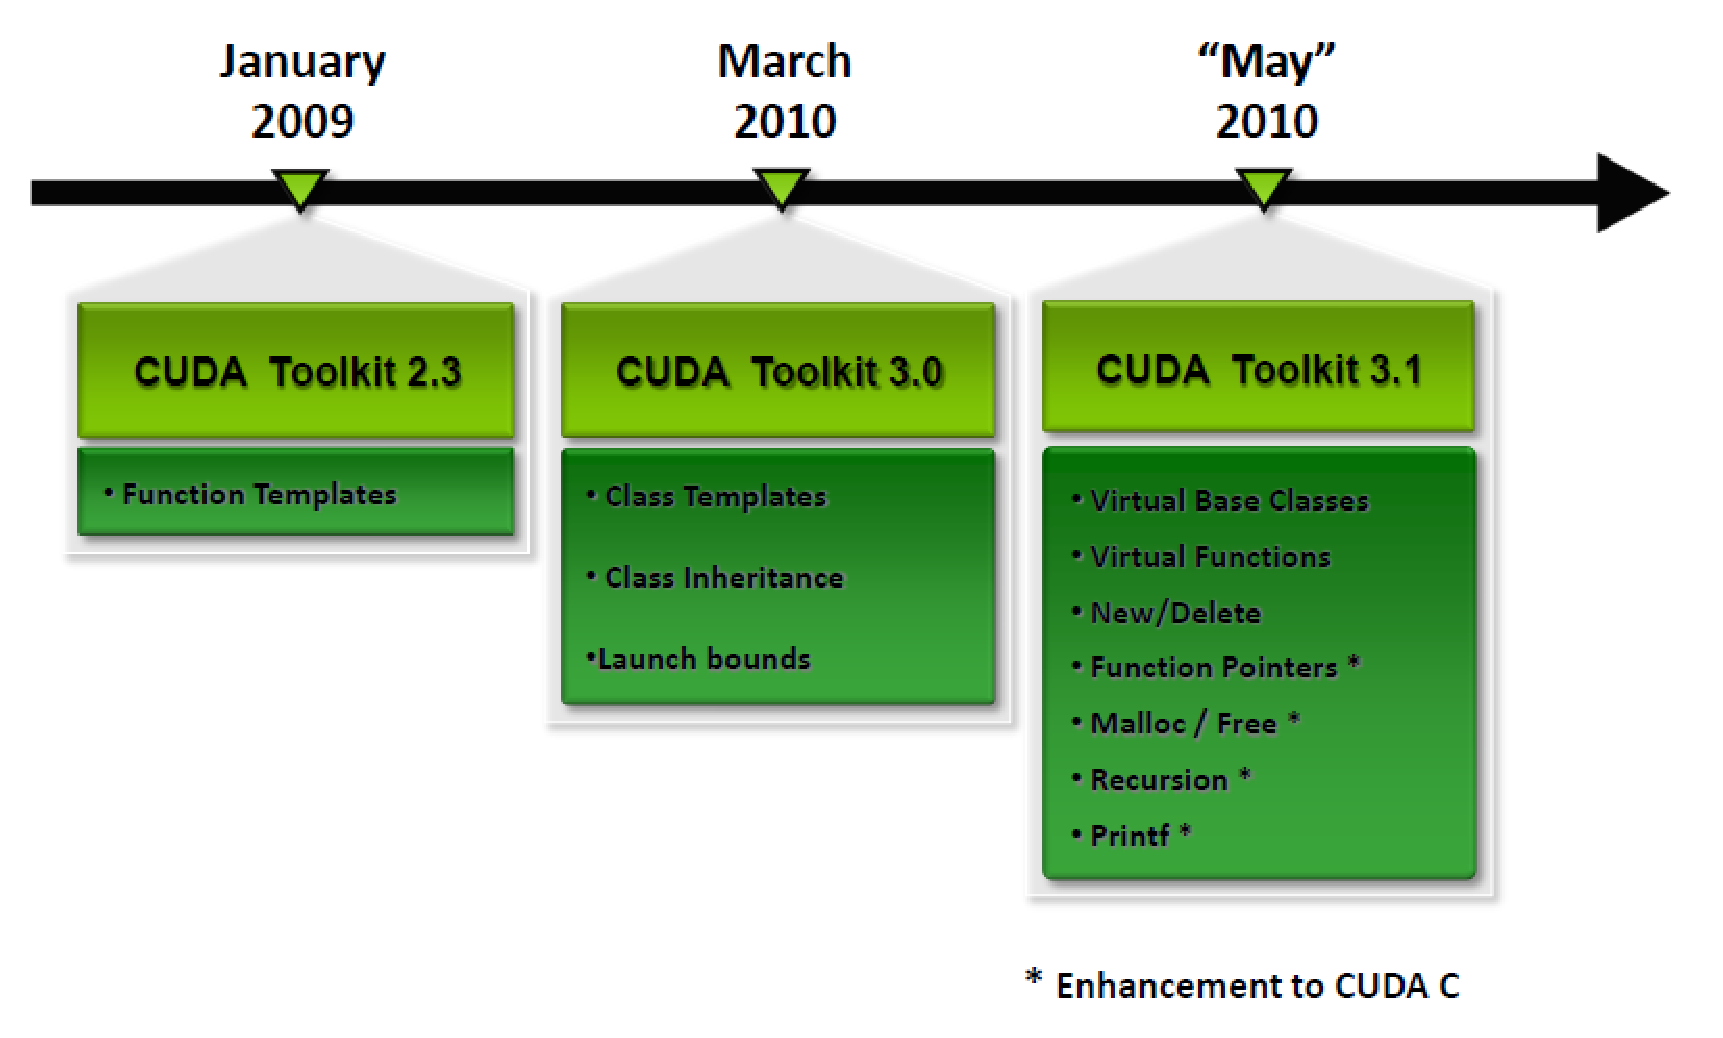
\includegraphics[height=5cm,
    angle=0]{./images/CUDA_C_new.eps}}
\caption{CUDA C improvements}
\label{fig:CUDA_C}
\end{figure}

% \section{Profiler {\bf computeprof}}
% \label{sec:profilers}

% This section describes how to use \verb!computeprof! to optimize the
% kernels. Suppose that you have a kernel, before you optimize it, you
% need to know the bottleneck in the kernel is due to
% \begin{enumerate}
% \item memory throughput
%   \begin{enumerate}
%   \item device memory: 144 GB/sec
%   \item constant memory: 
%   \end{enumerate}
% \item instruction throughput
%   \begin{enumerate}
%   \item 1030 GFLOPS (fp32), 515 GFLOPS (fp64)
%   \end{enumerate}
% \item latency
% \item combination of above
% \end{enumerate}

% Most of the counters reported by the profiler are derived from the
% calculation of a single SM, not entire GPU, except L2 and DRAM
% counters. So, it's not completely reflect the exact execution time. In
% a single run, it can only collect a few counters. Thus, a number of
% runs is requires when profiling more counters. Currently, in CUDA 3.2,
% the Visual Profiler automatically uses 9 runs (when you request all
% counters). If you use the command-line, you need to tell how many runs
% explicitly. 

% \begin{framed}
%   Two values for the same counter at different runs are not exactly
%   the same. So, it's implicitly to understand that ``two counters
%   being equal'' means ``with a small delta''. 

%   By default, kernel launches are non-blocking. However, in the
%   profiler, it's blocking so that the counters can be computed. With
%   blocking kernels, the \verb!CPU time! is the sum of the \verb!GPU
%   time! and the kernel launch overhead. 
% \end{framed}

%  Important statistics:
% \begin{itemize}
% \item Method 
% \item GPU usec
% \item \% GPU time
% \item glob mem read throughput (GB/s)
% \item glob mem write throughput (GB/s)
% \item instruction throughput
% \end{itemize}

\section{Fermi GPUs}

\subsection{Geforce 400 series, 500 series}
\label{sec:Fermi-based-Geforce}

Geforce 400 series (e.g. GTX 480) supports DirectX 11.0, OpenGL 4.4, and OpenCL
1.1. It is based on early Fermi chips (GF100): 448 cores. GF100 GPU can do
half-speed FP16 filtering.

Geforce 500 series (e.g. GTX 580) supports DirectX 12 and is based on newer
Fermi chips (GF110): 512 cores (fully enabled chips). GF100 GPU can do full
speed FP16 filtering and improved z-culling units.
\begin{enumerate}
  \item GF110: each SM has 32 SPs and 4 SFUs
  \item GF114/GF116/GF118: each SM has s48 SPs and 8 SFUs.
\end{enumerate}
Each SP can do 2 single-precision operations FMA or 4 single-precision SF per
clock. 
\subsection{Quadro}
\label{sec:Fermi-based-Quadro}

Nvidia Quadro 5000 is Fermi-based GPU.

\section{Page fault (memory addressing)}
\label{sec:page-fault}

When you allocate memory, you create a number of page tables on the page directory. The page tages
represent a region of continuous virtual memory address. 

If a page does not map to a physical memory region, and you try to access the memory address on that page, a
{\bf page fault} occurs.

In CPU, the pages are stored in host-side memory (i.e. CPU RAM).

\section{Reset Fermi memory without restart}
\label{sec:reset-fermi-memory}

This is the problem with earlier version of Nvidia driver. It has been resolved
in Nvidia 280.13. So, if you're still using older version of the driver, if
you get ``out of memory" error when running your CUDA program, you need to turn
off GUI
\begin{verbatim}
## Ubuntu 10.10 and earlier
sudo /etc/init.d/gdm stop

## Ubuntu 11.10 and later
service lightdm stop
\end{verbatim}
then you need to find out where nvidia.ko reside (notice the folder
with the same version with the driver that you're using, e.g. 
\begin{verbatim}
/var/lib/dkms/nvidia-current/270.18/build/nvidia.ko
\end{verbatim}
then you jump to this folder and type
\begin{verbatim}
rmmod nvidia.ko
insmod nvidia.ko

sudo /etc/init.d/gdm restart
\end{verbatim}
A better command line is
\begin{verbatim}
rmmod nvidia
modprobe nvidia
\end{verbatim}

If you get the error message 
\begin{verbatim}
ERROR: Module nvidia is in use
\end{verbatim}
then search for which process is using it
\begin{verbatim}
lsof -n -w -t /dev/nvidia*
\end{verbatim}
If it's the X-windows manager, we can call
\begin{verbatim}
sudo service lightdm stop
\end{verbatim}
or we need to follow the steps to find out which module depends on nvidia*, e.g.
\verb!<module>=nvidia!
\begin{verbatim}
/sbin/modinfo  <module> !show the dependency
lsmod <module>  !show the modules on the right-hand side depend on
         !the module on the left
rmmod -f <module>  ! to forcely remove the module (only work if
             !CONFIG_MODULE_FORCE_UNLOAD is enabled in the kernel
modprobe -rf <module>  ! more powerful than rmmod

\end{verbatim}
E.g.:
\begin{verbatim}
/sbin/modinfo nvidia | grep -v -e alias: -e parm:
filename:       /lib/modules/2.6.25.18-0.2-default/weak-updates/nvidia.ko
license:        NVIDIA
depends:        i2c-core
supported:      external
vermagic:       2.6.25.11-0.1-default SMP mod_unload
\end{verbatim}

\section{Device management}
\label{sec:device-management}

To tell the preferred cache configuration for the current device, i.e.
16/48KB or 48/16KB configuration for L1 cache/shared memory, we use
\verb!cudaDeviceGetCacheConfig()!
\begin{lstlisting}
integer cudaDeviceGetCacheConfig(cacheconfig)
  integer, intent(out) :: cacheconfig
\end{lstlisting}
It can be \verb!cudaFuncCachePreferNone!,
\verb!cudaFuncCachePreferShared! or \verb!cudaFuncCachePreferL1!. 

There are two tools we can use: \verb!nvidia-smi! and NVML (Nvidia Management
Library).\footnote{\url{https://developer.nvidia.com/nvidia-management-library-nvml}}

\begin{mdframed}
There are two types of ECC errors: single-bit and double-bit.

Single-bit ECC errors are correctable; while double-bit ECC errors can be
detected, but are uncorrectable. Texture memory error can be corrected by
resend, and if this resend fail, then the error becomes uncorrectable.  The
errors are available at two timescales (volatile or aggregate).

\end{mdframed}

\verb!nvidia-smi! is the Linux utility for Nvidia's system management,
which support the following devices
\begin{verbatim}
Supported products:
Tesla: S1070, S2050, C1060, C2050/70, M2050/70/90, X2070/90
Quadro: 4000, 5000, 6000, 7000 and M2070-Q
Other: All other products are unsupported
\end{verbatim}
\url{http://briot-jerome.developpez.com/fichiers/blog/nvidia-smi/list.txt}

Options
\begin{verbatim}
    -pm,  --persistence-mode=   Set persistence mode: 0/DISABLED, 1/ENABLED
    -e,   --ecc-config=         Toggle ECC support: 0/DISABLED, 1/ENABLED
    -p,   --reset-ecc-errors=   Reset ECC error counts: 0/VOLATILE, 1/AGGREGATE
    -c,   --compute-mode=       Set MODE for compute applications:
                                0/DEFAULT, 1/EXCLUSIVE_THREAD,
                                2/PROHIBITED, 3/EXCLUSIVE_PROCESS
\end{verbatim}

\begin{enumerate}
  \item If the devices \verb!/dev! are not created at boot, then we can
  initialize the devices and create the proper devices folder using
\begin{verbatim}
nvidia-smi -L


>>
GPU 0: GeForce GTX 480 (UUID: GPU-adce5c8e-08b3-ba91-dcba-3caac9dc43e9)
GPU 1: Tesla C2050 (UUID: GPU-14612672-e1f2-b70c-4fbb-a16adfda0ac5)
GPU 2: Tesla C2050 (UUID: GPU-430d4650-7de5-bf6f-0ef3-016aeefa81a4)
\end{verbatim}

  \item To set GPU to persistent mode (keeping the driver loaded even when no
  applications are accessing the card)
\begin{verbatim}
nvidia-smi -pm 1
\end{verbatim}

  \item  To list all available data to a particular GPU, e.g. GPU zero-th
\begin{verbatim}
nvidia-smi -i 0 -q

  // or just to check a few fields
nvidia-smi -i 0 -q -d MEMORY,UTILIZATION,POWER,CLOCK,COMPUTE

>>  This is the result from an idle card
==============NVSMI LOG==============

Timestamp                           : Thu Aug  7 22:22:04 2014
Driver Version                      : 319.60

Attached GPUs                       : 3
GPU 0000:03:00.0
    Product Name                    : Tesla C2050
    Display Mode                    : Disabled
    Display Active                  : Disabled
    Persistence Mode                : Disabled
    Accounting Mode                 : N/A
    Accounting Mode Buffer Size     : N/A
    Driver Model
        Current                     : N/A
        Pending                     : N/A
    Serial Number                   : 0321410032798
    GPU UUID                        : GPU-14612672-e1f2-b70c-4fbb-a16adfda0ac5
    VBIOS Version                   : 70.00.2B.00.02
    Inforom Version
        Image Version               : N/A
        OEM Object                  : 1.0
        ECC Object                  : 1.0
        Power Management Object     : N/A
    GPU Operation Mode
        Current                     : N/A
        Pending                     : N/A
    PCI
        Bus                         : 0x03
        Device                      : 0x00
        Domain                      : 0x0000
        Device Id                   : 0x06D110DE
        Bus Id                      : 0000:03:00.0
        Sub System Id               : 0x077110DE
        GPU Link Info
            PCIe Generation
                Max                 : 2
                Current             : 1
            Link Width
                Max                 : 16x
                Current             : 16x
    Fan Speed                       : 30 %
    Performance State               : P12
    Clocks Throttle Reasons         : N/A
    Memory Usage
        Total                       : 2687 MB
        Used                        : 6 MB
        Free                        : 2681 MB
    Compute Mode                    : Default
    Utilization
        Gpu                         : 0 %
        Memory                      : 0 %
    Ecc Mode
        Current                     : Enabled
        Pending                     : Enabled
    ECC Errors
        Volatile
            Single Bit            
                Device Memory       : 0
                Register File       : 0
                L1 Cache            : 0
                L2 Cache            : 0
                Texture Memory      : N/A
                Total               : 0
            Double Bit            
                Device Memory       : 0
                Register File       : 0
                L1 Cache            : 0
                L2 Cache            : 0
                Texture Memory      : N/A
                Total               : 0
        Aggregate
            Single Bit            
                Device Memory       : N/A
                Register File       : N/A
                L1 Cache            : N/A
                L2 Cache            : N/A
                Texture Memory      : N/A
                Total               : 0
            Double Bit            
                Device Memory       : N/A
                Register File       : N/A
                L1 Cache            : N/A
                L2 Cache            : N/A
                Texture Memory      : N/A
                Total               : 309590
    Retired Pages
        Single Bit ECC              : N/A
        Double Bit ECC              : N/A
        Pending                     : N/A
    Temperature
        Gpu                         : 51 C
    Power Readings
        Power Management            : N/A
        Power Draw                  : N/A
        Power Limit                 : N/A
        Default Power Limit         : N/A
        Enforced Power Limit        : N/A
        Min Power Limit             : N/A
        Max Power Limit             : N/A
    Clocks
        Graphics                    : 50 MHz
        SM                          : 101 MHz
        Memory                      : 135 MHz
    Applications Clocks
        Graphics                    : N/A
        Memory                      : N/A
    Default Applications Clocks
        Graphics                    : N/A
        Memory                      : N/A
    Max Clocks
        Graphics                    : 573 MHz
        SM                          : 1147 MHz
        Memory                      : 1500 MHz
    Compute Processes               : None
\end{verbatim} 

NOTE: M-series GPUs doesn't report the temperature to \verb!nvidia-smi!, as the
temperature data is reported directly to IPMI, allowing the system's BMC to
properly control chassis cooling. Only desktop series, C-series Tesla or Quadro
do report to \verb!nvidia-smi!.

  \item To reset ECC error count
\begin{verbatim}
nvidia-smi -i 1 -p 1 
\end{verbatim} 
NOTE: \verb!-i ! accepts device ID, \verb!-p! accepts either 0 (VOLATILE) or 1
(AGGREGATE).

\end{enumerate} 
\url{http://www.microway.com/hpc-tech-tips/nvidia-smi_control-your-gpus/}

\url{https://developer.nvidia.com/sites/default/files/akamai/cuda/files/CUDADownloads/NVML_cuda5/nvidia-smi.4.304.pdf}


\subsection{CU}
\label{sec:cu}

Instruction issues are relatively simple compared to that of CPU. Instructions
are issued per {\it warp} consecutive threads, with $warp=32$ in Fermi. So, to
maximize the performance, threads in a warp should execute the same instruction.
By that, we only need to issue the instruction once. When there is code path
divergence; some threads execute instructions different from the others in the
same warp. This will, eventually, decrease the performance.

However, code divergence is not an issue if it's not from the same
warp. 

Instructions are not prefetch; so there is no overhead on switching
threads. 

A CUDA core (Compute Unit) has 
\begin{enumerate}
  \item Dispatch port
  \item Operand Collector
  \item 1 FP unit + 1 INT unit
  \item 1 result queue
\end{enumerate}
which can compare, move data, do arithmetic, or logic operations. 



\subsection{Pipeline}
\label{sec:pipeline}

Memory access are issued as vector of 32 addresses of 4-byte data. So,
ideally, if consecutive threads in a single warp access adjacent data,
we only need a single memory request. For double precision data, we
need at least 2 memory access. As the result, the transaction sizes
vary from 32 bytes (= 1x4byte) to 128 bytes (= 32x4byte).

The starting memory for each read should be a multiple of 64. So,
memory coalescing is very important. 

\subsection{Instruction throughput}
\label{sec:instr-thro}

each warp can issue
\begin{enumerate}
\item  2 fp32 pipes for 2 cycles
\item  2 int32 pipes for 2 cycles
\item 1 fp64 pipe for 4 cycles
\item 1 special-function (SFU) pipe for 16 cycles
\end{enumerate}
Instructions from two different warps will be issued to 2 different
pipes automatically. 


\subsection{Caches (L1/L2 cache, constant-cache)}
\label{sec:caches}

Lifetime of data in L1 cache is very short. Each time data is loaded
in L1 in group of 128-byte line and this apply to L2 cache as well. If
we want a smaller granularity, we can choose 32-byte; yet without
possibility of using L1, i.e. L1 is idle. However, this setting is not
coherent across multiprocessors, i.e. one MP may use 128-byte line and
another one use 32-byte line. 
\begin{enumerate}
\item Using 32B or 128B is compiler option
\item Using 16KB/48KB of L1 cache/shared memory is configurable from
  source code and per kernel. 
\end{enumerate}

Previous generation use 16 banks of memory. Fermi use 32 banks of
memory (each with 32-bits wide); thus avoiding bank conflicts with
64-bit and 128-bit words.

For constant-cache memory, read Sect.\ref{sec:constant-memory}.

Zero-copy memory from host, it will automatically loaded into L2
also. 

GDDR5: Transaction size is a multiple of 128-B for Fermi, and probably 256B
or 512B in next generations.

\subsection{Programming}
\label{sec:programming}

2D/3D thread blocks should be a multiple of 32 in ``wide''. As a
result, data should be a multiple of 32 in the fastest-varying
dimension. 


\subsection{Limitations}
\label{sec:Limitation}

{\bf LIMITATIONS}: These below are not doable on Fermi and CUDA 3.x
\begin{enumerate}
\item Applications that need entire data to be ``in
core'' and data size is larger than total GPU global memory.

\item Data transfer between GPUs. They must use CPU memory as the
  intermediate. 

\item I/O related task cannot use data residing on GPU. They must be
  on CPU first.
\end{enumerate}

To copy data between CPU and GPU global memory, we can use
\begin{itemize}
\item blocking memcopy
\begin{lstlisting}{lang="C"}
cudaMemcpy( void *dst, void *src, size_t nbytes,
     enum cudaMemcpyKind direction);
\end{lstlisting}
with \verb!enum cudaMemcpyKind!
\begin{verbatim}
cudaMemcpyHostToDevice
cudaMemcpyDeviceToHost
cudaMemcpyDeviceToDevice
\end{verbatim}
returns after the copy is complete
blocks CPU thread until all bytes have been copied
doesn't start copying until previous CUDA calls complete

\item Non-blocking memcopies are provided

\end{itemize}



\chapter{Kepler architecture}
\label{chap:Kepler}


Different Tesla-Kepler family: Tesla K10 (2x GK104), Tesla K20X (GK110), Tesla
K40 (GK110b) (Sect.\ref{sec:Tesla-Kepler}). 
Tesla K20 is available in 6GB, 12GB, and 24GB of ECC memory DDR5. 
\footnote{\url{http://technewspedia.com/more-details-of-nvidia-tesla-cgpu-k20-gk110/}}

Kepler (GK104) will be the first generation of Nvidia GPU to support DirectX
12.0 (Fermi support DirectX 11.0) and uses 28nm technology,
Fig.\ref{fig:kepler_roadmap}. Windows 8 will support DirectX 11.1.
Kepler is designed to improve performance per watt. Using 28nm technology, with
other GPU architecture modifications, Kepler helps lowering power consumption.
\begin{enumerate}
  \item Kepler-based videocard can connect 3 different monitors:
  full-size HDMI port, dual-link DVI and VGA connection.

  \item Kepler-based chips are built using 28 nm technology.

  \item A single clock rate is used for any taks of GPU cores (regardless of
  shading or general-computing kernel) (Sect.\ref{sec:clock-cycles-speeds}). 
  The unified clock rate is called the {\bf base clock} .
  
  In earlier generations, the goal of using a faster shader clock for the
  execution units is to achieve high throughput while using fewer copies of the
  execution units. However, the clocking logic of the faster cores is more
  power-consumption. In Kepler, the goal is to achieve more performance per
  watt, not performance per core like in Fermi. So, Kepler introduces more
  cores, while making the cores run at a lower speed.
  
  This brings up efficiency (i.e. two Kepler cores use about 90\% of the power
  by one Fermi core, and the reduction in clock speed brings a 50\% reduction in
  power consumption). However, when needed, GPU core can run at a faster rate by
  using a dynamic clock speed adjustment which is controlled by GPU Boost 1.0
  (from GTX 600 series) and GPU Boost 2.0 (from GTX 700 series), which makes
  real-time change to clock speed for maximizing performance by increasing base
  clock until the graphics card hits a predetermined Temperature Target.
  Performance increase: 3-7\% on GPU Boost 1.0
  \footnote{\url{http://www.geforce.com/hardware/technology/gpu-boost-2/technology}}.

  \item Then the new texture handling mechanism
  (Sect.\ref{sec:Kepler_texture-handling}). In Kepler, the memory clock is now 6
  GHz, compared to 4GHz in Fermi and 2.5GHz in GT200. NOTE: The theoretical
  limitation of GDDR5 memory is 7GHz.

  \item A dedicated hardware (FP64 ALU) to handle double-precision. In Fermi,
  two FP32 units work together to do double-precision.
    
  \item SM (in Fermi) is replaced by the next generation Streaming
  Multiprocessor, ``SMX'' (Sect.\ref{sec:Kepler_SMX}). This is the key to Kepler.
  Each SMX in Kepler has 192 cores, compared to 32 cores in SM of Fermi. 
  The architecture is Power-aware SMX. It thus results power down and
  performance up (using Turbo Boost).  

  \item Kepler GPU is PCIe Gen3 compliant, i.e. it can run on PGI-e Gen3 ports.
  However, not all Kepler-based products support PCI-e Gen3 speeds. Tesla K10
  and K40 support PCIe 3.0, Tesla K20 and K20X do not.
  \footnote{\url{http://docs.nvidia.com/cuda/kepler-tuning-guide/\#pcie-30}}

  
However, the graphics card will not run on PCI-e Gen3 mode, as Nvidia didn't
implement the driver support for X79 chipset motherboards (X79/SNB-E systems or
Sandy Bridge-E HEDT). PCI-Express 3.0 x16, for now, might only run on upcoming
"Ivy Bridge" Core systems, running on motherboards with PCI-Express 3.0
compliant components.
\footnote{\url{http://www.techpowerup.com/162942/geforce-gtx-680-release-driver-limits-pci-express-to-gen-2-0-on-x79-snb-e-systems.html}}
  
Recently, Nvidia released the patch to run PCI-e Gen3 on Sandybridge
motherboard. Use this patch along with the latest GeForce drivers to enable
PCI-Express Gen 3.0 mode for GeForce Kepler-based graphics cards, on Intel Sandy
Bridge-E (X79) systems.
\footnote{\url{http://www.techpowerup.com/downloads/2148/nvidia-geforce-kepler-pcie-3-0-mode-enabling-patch-for-sandy-bridge-e-systems/}}
  
  \item New APIs: Compute-capability CC 3.0
  
\end{enumerate}
White paper: \url{http:///www.nvidia.com/object/nvidia-kepler.html}


\begin{figure}[hbt]
  \centerline{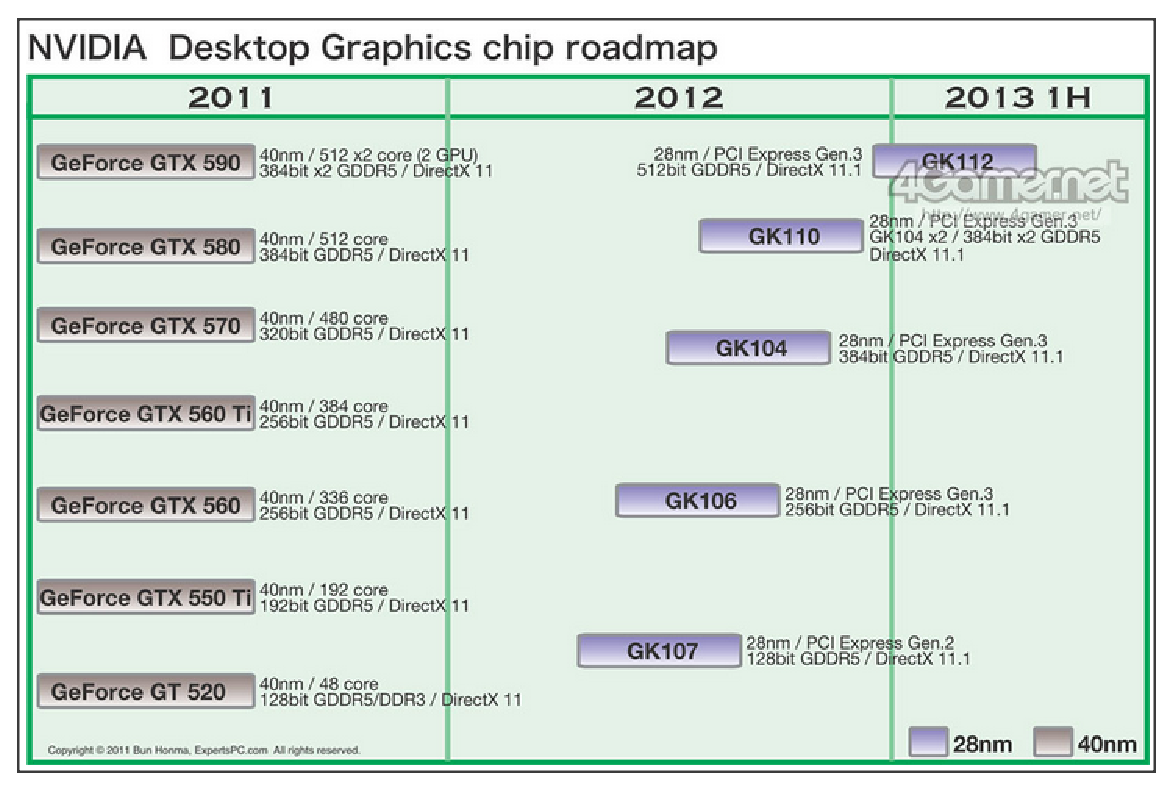
\includegraphics[height=7cm,
    angle=0]{./images/kepler_roadmap.eps}}
  \caption{Roadmap of Kepler 28nm technology}
  \label{fig:kepler_roadmap}
\end{figure}


\section{Kepler GPUs}

A good comparison between GPU chips is given in
Fig.\ref{fig:compare_CUDA-capable-GPUchips}.

\url{http://www.tomshardware.com/reviews/geforce-gtx-680-review-benchmark,3161-2.html}

\begin{figure}[hbt]
  \centerline{\includegraphics[height=5cm,
    angle=0]{./images/CUDA_GPU_comparison.eps}}
  \centerline{\includegraphics[height=5cm,
    angle=0]{./images/Compare_GTX680_GTX580.eps}} 
  \caption{GPU comparison}
\label{fig:CUDA_GPU_comparison}
\end{figure}

\subsection{GK104}
\label{sec:GK104}

{\bf GK104} is the first GPU chip based on the Kepler architecture to run on
PCIe Gen3. GK104 chip is designed for performance GPU, targers to mid-end users.
GK104 has
\begin{itemize}
  \item  3.54 billion transistors on 294 mm$^2$ die with 8 SMX, each with
192 CUDA cores, i.e. totally 1536 CUDA cores.
  \item PCI-e Gen3 (44 mm$^2$)
  \item 256-bit memory bus (60 mm$^2$)
  \item 4 GPC (each 37 mm$^2$)
  \item one GigaThread (6 mm$^2$)
  \item 512 KB L2 cache + 32 ROPs (37 mm$^2$)
  
  \item GRAPHICS: 80-96 texture units (TMUs). 
  \item The base clock is 915 MHz, which can be boost to
1010 MHz (using Turbo Boost 1.0), and memory clock 6.008 GHz GDDR5.
Expected performance: more than 2TFLOPs in single-precision. 

  \item GK104 requires CUDA 3.0 minimum. 
  
  \item The fraction of FP64 is 1/24 FP32.
\end{itemize} 
The first videocard product to use GK104 is Geforce GTX 680 with 2
GB 1.502 GHz RAM, running at 1006 MHz (boost to 1058 MHz). Using the formula in
Sect.\ref{sec:chip-memory}, the peak theoretical data throughput is 192 GB/s.  


% with 640-768 CUDA cores; memory interface 256-bit or 384-bits.

There are variants of GK104, i.e. the cut-down versions: {\bf GK104-335-A2} with
7 SMX (1344 CUDA cores, 256-bit memory bus, 112TMU, 32 ROPs), {\bf GK104-400-A2}
with 6 SMX (192-bit memory bus), {\bf GK104-425-A2}.
The videocards Geforce GTX 670 use GK104-335-A2, 2GB GDDR5, core-clock 915-950
MHz, memory clock 1.25 GHz.
\footnote{\url{http://www.tweaktown.com/news/23836/nvidia_preps_two_more_kepler_gk_104_based_cards_gtx_660_and_670/index.html}}
The videocards Geforce GTX 680 use GK104-400-A2.
The videocards Geforce GTX 770 use GK104-425-A2 (425 implies some slight
optimisation and changes).

Geforce GTX 690 was first available around May-2012, a videocard combining two
fully-enabled GK104-chips interconnected using SLI, giving total 2x1536 CUDA
cores, 2x128 TMUs, 2x32 ROPs, FP64 units (is about 1/24 FP32 units). GTX 690 TDP
is 300 watts.

GK104 has
\begin{enumerate}
  \item PCI-e Gen3 Host Interface
  \item 4 256-bit memory controllers
  \item 4 GPC with each GPC has 2 SMX block. So, totally it has 8 SMX blocks.
  XMS runs at the base-clock. 
  \item L2 cache shared by all CUDA cores.
  \item With 4 memory controller, GK104 has 4x128=512KB L2-cache and 32 ROP units. It
means it can do 32 color samples at once. 
\end{enumerate}




\subsection{GK107}
\label{sec:GK107}

GK107 chip is for entry GPU with PCI-e Gen2 and uses 1.3 billion transistors. 
GK107 has only 2 SMX units (giving totally 384 CUDA cores). GK107 has 32 texture
units and 16 ROPs. The memory bus is 128-bit (support DDR3 and GDDR5 memory).
Base-clock is 900 MHz, and memory clock is 900 MHz. The chip's TDP is 65 watts (i.e. no
external power connection is required).

The first videocard to use GK107 chip is GeForce GT 640 (1GB DDR3).

\subsection{GK106}

GK106 is built on 210 mm$^2$ die. Its memory bus is 192-bit (GDDR5 memory
interface). GK106 features 2 raster engines (RPC), 4 SMX (i.e. 768 CUDA cores),
24 ROPs, and 64 TMUs. The base-clock is 1006 MHz, and can be boost to 1359 MHz.
 
The first videocard to use GK106 chip is GeForce GTX 660 with TDP
130 watts (Sept-2012).



\subsection{GK110 (flagship), GK110b}
\label{sec:GK110}
\label{sec:GK110b}

Unlike Fermi-based GPU family whose flagship GPU chip is GF100, in Kepler, the
flagship GPU chip is GK110 (not GK100) which is considered a 28nm version of
GF110 (a major revision of GF100). {\bf GK110 requires minimum CUDA 3.5}
instruction sets (Sect.\ref{sec:CC3.5}).

Even though GK104 is powerful (Sect.\ref{sec:GK104}), it's not designed for
general-purpose computing, i.e. no ECC memory protection, very low (only 1/24)
FP64/FP32 rate, few load/store units in comparison to ALU (CUDA cores), low L1
bandwidth per ALUs (0.33 Byte/FLOP for 32-bit operations, 0.66 Byte/FLOP for
64-bit operations)
\footnote{\url{http://www.ilsistemista.net/index.php/hardware-analysis/27-big-kepler-gk100-speculations.html}}

A complete GK110 GPU has 
\begin{itemize}
  \item  about 550 mm$^2$, with total 7.1B transistors. 
  
  GK110 can accommodate 15 SMX units (Sect.\ref{sec:SMX} - an extension concept
  from SM (streaming multiprocessor)). However, only 14 SMX are
  activated, as one SMX is disabled, giving total 14x192 = 2,688 CUDA cores
  and 14x16=224 TMUs available (NOTE: GTX 680 has 128 TMUs). 
  
  The variant GK110-301-B1 ({\bf GK110b}) is the GPU chip (having a larger die
  561 mm$^2$ and 7.08 billion transistors) with full 15 SMX units, i.e.
  giving total 2880 CUDA cores. GK110B is being used to build Tesla K40
  (Sect.\ref{sec:K40}).


  \item FP64/FP32 ratio is 1/3: Every 3 CUDA cores has 1 FP64 double-precision
  unit. FP64 in GK110 can do $> 1$ TFLOPs.

So, in an SMX, it has 192*1/3=64 DP units. With this ratio, GK110 can deliver
power of calculation in double-precision about 50\% - 85\% compared to power in
single-precision (FP32).
\footnote{\url{http://technewspedia.com/more-details-of-nvidia-tesla-cgpu-k20-gk110/}}
  
  \item memory interface: 384 bits
  
  \item connect to motherboard using PCI-e Gen2
  
  \item GK110 has 1.5MB L2 cache, with the number of 32-bit register per SMX is 65,536.

Compared to GF100 (Sect.\ref{sec:gf100-fermi}, the number of cores is 6x, while
the number of registers only double. So, it's important to limit the number of
registers/thread when writing CUDA kernels.
  
\end{itemize}


To improve performance per watt, the clock is down from 2x in Fermi to 1x clock
in Kepler.
\begin{verbatim}
For login: area is 1.0x, power is 1.0x
   Kepler: 1.8x and 0.9x
For clocking: area is 1.0x, power is 1.0x
   Kepler: 1.0x and 0.5x
\end{verbatim}
This show how they do power saving.

Selections:
\begin{enumerate}
  
  \item Geforce GTX Titan (Feb 2013) is the first videocard to use GK110 chip.
  It uses 6 GB of memory. Tesla K20 is using GK110 (Sect.\ref{sec:K20}).

  \item GeForce GTX 780Ti is the first videocard (Sep-2013) to use GK110b chip,
  yet with reduced double-precision.
  
GeForce GTX 780 Rev. 2 also use GK110b, yet has some shading units disabled,
i.e. only 2304 shading units (CUDA cores, running at 863 MHz, which can be
boosted up to 902 MHz), 192 TMUs (texture mapping units) and 48 ROPs, and
3,072MB 1502 MHz GDDR5 memory interconnected using 384-bit memory interface.

  \item 
\end{enumerate}


\subsection{GK100/GF112}

SUMMARY: GK100/GK112 has 1024 CUDA cores, with 512-bit GDDR5 Memory interface;
memory bandwidth ??? GB/s. GRAPHICS: 128 textures units (TMUs), 64 raster operators
(ROP). Performance:

\subsection{GK20A}
\label{sec:GK20A}

GK20A is the Kepler-based graphics core found within the Tegra K1 SoC
(Sect.\ref{sec:Tegra_nvidia}). GK20A has 192 GPU cores. In addition to the GPU
chip, Tegra K1 also features either a 64-bit ARM or Nvidia's Project-Denver
processor. Project-Denvor process is now called 32-bit quad-core, 4-Plus-1
Cortex-A15
processor.\footnote{\url{http://www.phoronix.com/scan.php?page=news_item&px=MTU2MDg}}

\subsection{GK210}
\label{sec:GK210}

GK210 is the third revision of GK110 (Sect.\ref{sec:GK110}). There are major
feature changes, Fig.\ref{fig:GK110_mainstreams}. Even though the memory bus
interface do not change (i.e. 384-bit memory interface), it has
\begin{enumerate}
  \item only 13 SMX are activated, i.e. giving total 2496 cores
  
  \item each SMX (Sect.\ref{sec:SMX}) has
  \begin{itemize}
 
    \item double the registers (compared to GK110, GK110b): 512KB registers,
   i.e.   131,072 32-bit registers.
  
    \item double shared-mem/L1 cache (compared to GK110, GK110b): 128KB total 
  
  \end{itemize}
\end{enumerate} 
The small change here improves the data throughput within an SMX,
serving to improve efficiency and keep the CUDA cores working more often. 

\begin{figure}[hbt]
  \centerline{\includegraphics[height=5cm,
    angle=0]{./images/GK110_mainstreams.eps}}
  \caption{The mainstream GPU for Tesla Kepler chip}
  \label{fig:GK110_mainstreams}
\end{figure}

The new GK210 is being used to produce Tesla Kepler K80 (Sect.\ref{sec:K80}).



\section{non-Tesla Kepler-based products}
\label{sec:Kepler-non-Tesla}

For Kepler-based Tesla products, see Sect.\ref{sec:Tesla-Kepler}.

\subsection{-- Geforce 600, 700}
\label{sec:Kepler-based-Geforce}

Geforce 600 series use GK104, GK106, GK107 and GK208.

Geforce 700 series use GK107, GK110, GK208 and GM107 (Maxwell). 

Geforce GTX Titan and Geforce GTX 780 were released in 2013. In GTX Titan
(Black), double-precision can be either 1/3 or 1/24 of single-precision
depending on the user-selected configuration. Other Kepler's GPU,
double-precision performance is fixed 1/24 of single precision. Geforce 700
series double precision performance is 1/32 of single-precision
performance.\footnote{\url{http://www.anandtech.com/show/7764/the-nvidia-geforce-gtx-750-ti-and-gtx-750-review-maxwell/5}}

\begin{figure}[hbt]
  \centerline{\includegraphics[height=5cm,
    angle=0]{./images/compare_CUDA-capable-GPUchips.eps}}
\caption{Compare GF100, GF104, GK110, and GK104
\footnote{\url{http://www.tomshardware.com/reviews/geforce-gtx-titan-gk110-review,3438-2.html}}}
\label{fig:compare_CUDA-capable-GPUchips}
\end{figure}

\subsection{-- Quadro K5000, K6000}
\label{sec:Kepler-based-Quadro}

Quadro K5000 is first Kepler-based Quadro GPU, successor to Fermi-based Quadro
5000 (Sect.\ref{sec:Fermi-based-Quadro}). Quadro K5000 uses GK104 chip
(Sect.\ref{sec:GK104}); while Quadro K6000 uses GK110 chip
(Sect.\ref{sec:GK110}).

\begin{figure}[hbt]
  \centerline{\includegraphics[height=5cm,
    angle=0]{./images/Quadro-Kepler.eps}}
  \centerline{\includegraphics[height=5cm,
    angle=0]{./images/Quadro2-Kepler.eps}}
  \caption{Compare between Kepler-based Quadro (K5000) vs. Fermi-based Quadros
  (Quadro 6000 and 5000)}
\label{fig:Quadro-Kepler}
\end{figure}

Quadro K6000 is the second-line Kepler-based Quadro GPU, successor to
Fermi-based Quadro 6000 (Sect.\ref{sec:Fermi-based-Quadro}). 



\section{Tesla Kepler board}
\label{sec:Tesla-Kepler}

For Kepler-based non-Tesla products, see Sect.\ref{sec:Kepler-non-Tesla}.

There are 3 early members in the Tesla-Kepler family GPGPU card (board),
Fig.\ref{fig:Tesla_Kepler_comparison}. Now, there is a new one: Tesla K80
(Sect.\ref{sec:K80}).

\begin{figure}[hbt]
  \centerline{\includegraphics[height=5cm,
    angle=0]{./images/Tesla_Kepler_comparison.eps}}
  \caption{Technical specification for Tesla Kepler}
  \label{fig:Tesla_Kepler_comparison}
\end{figure}

\subsection{Tesla K10}
\label{sec:K10}

Tesla K10 is optimized for single-precision, using two GK104 chip
(Sect.\ref{sec:GK104}), which can deliver 2x performance compared to Tesla M2090
GPU for single-precision applications.

\subsection{Tesla K20 (K20m, K20c) and Tesla K20X}
\label{sec:K20}

Tesla K20 are designed for double-precision (DP64), based on GK110 chip
(Sect.\ref{sec:GK110}), with 320-bit memory interface. 

Tesla K20 has less CUDA cores, i.e. 2496, and use 5.2GHz 5GB GDDR5 memory
of 320-bit memory interface giving 208 GB/s. Tesla K20X is a minor revision with
14 SMX activated and 5.2GHZ 6GB GDDR5 memory of 384-bit memory interface giving
250 GB/s.

\begin{itemize}
  \item K20X (with 14 SMX, i.e. 2688 CUDA cores): 3.95 TFLOPs on
  single-precision and 1.31 TFLOPs on double-precision
  
Passive heatsink relies on chassis cooling of specially-designed GPU servers  
It has 235W TDP.
  
  \item K20 (with 13 SMX): 3.52 TFLOPs on single-precision and 1.17 TFLOPS on
  double precision.

Passive (K20m) or active (K20c) heatsink options for servers and workstations
It has 225W TDP.

\end{itemize}
\url{https://www.microway.com/hpc-tech-tips/nvidia-tesla-k20-gpu-accelerator-kepler-gk110-up-close/}

\subsection{Tesla K40}
\label{sec:K40}

Tesla K40 was introduced in SC'2013 conference as the first fully-enabled Kepler
Tesla card. It is based on GK110B variant of NVIDIA's GPU
(Sect.\ref{sec:GK110}). Tesla K40 is designed for large-scale double-precision
simulation, which has 12 GB of {\bf 6GHz GDDR5 memory} (memory bandwidth is 288
GB/s, Fig.\ref{fig:Tesla_K40_benchmark}), and full 15 SMX units, i.e. 2880 cores
that can deliver 4.29 TFLOPs for single-precision and 1.43 TFLOPs on
double-precision.

\begin{mdframed}

Memory bandwidth of 288GB/s
 \footnote{\url{http://www.pcper.com/news/General-Tech/NVIDIA-Tesla-K40-GK110b-Gets-Career-and-more-vRAM}},
is 50\% higher than GTX 680 2GB and about the same as ATI/AMD HD 7970 3GB.

\end{mdframed}

\begin{figure}[hbt]
  \centerline{\includegraphics[height=5cm,
    angle=0]{./images/Tesla_K40_benchmark.eps}}
\centerline{\includegraphics[height=5cm,
    angle=0]{./images/Tesla_K40_benchmark2.eps}}    
  \caption{Brief overview of K40}
  \label{fig:Tesla_K40_benchmark}
\end{figure}

Since Tesla K40, the GPU Boost 2.0 is added which was previously only available
in Geforce cards as GPU Boost 1.0, Fig.\ref{fig:GPU_Boost}. Tesla 40 base clock
is 745 MHz, and can jump to 2 different boost clock: 810 MHz or 875 MHz. K40 can
deliver 20-40\% increase in performance in some applications compared to K20.
There are certain limitations to GPU Boost 2.0. Tesla K40 had to obey its TDP
(235W TDP), but operators could select which of 3 clockspeeds they wanted,
picking the one that comes closest to (but not exceeding) TDP for the best performance. The GPU
Boost in Tesla K80 is better (Sect.\ref{sec:K80}).

\begin{figure}[hbt]
  \centerline{\includegraphics[height=3.5cm,
    angle=0]{./images/GPU_Boost.eps}}
  \caption{GPU Boost 2.0 can automaticaly scale up frequencies based on
  voltage, temperature and power target}
  \label{fig:GPU_Boost}
\end{figure}

\subsection{Tesla K80}
\label{sec:K80}

Tesla K80 has been introduced at SC'2014 conference,
Fig.\ref{fig:Tesla_K80_comparison}. It is a dual-GPU card using two GK210
(Sect.\ref{sec:GK210}), thus doubles the number of transistors, i.e. 2 x 7.1B,
compared to GK110. 

\begin{mdframed}
Using dual cards has been done before (Tesla K10, or GeForce Titan Z), but this
is different as only 13 out of 15 SMX are enabled on each GPU, i.e. giving the
combined  4,992 CUDA cores enabled. 

The GK210 chip in Tesla K80 operates at 562MHz (normal) and 875MHz (boost
state). This allows Nvidia to put two high performance GPU chips within 300W TDP
(i.e. 150W per GPU system) is no small achievement in and of itself, though for
this reason GPU Boost plays a big part in making the overall product viable.
The worst case scenario is that it's only 2\% more energy efficient than K40
(Sect.\ref{sec:K40}) while the best case is 59\%, with the realistic case being
somewhere in the middle.
\end{mdframed}


Tesla GK80 specs:
\begin{enumerate}
  
  \item  The FP64/FP32 ratio is still 1/3: but with more cores, it can deliver
  8.74 TFLOPS in single and 2.91 TFLOPS in double precision,
  Fig.\ref{fig:Kepler_performance}.

Compared to Tesla K40 (Sect.\ref{sec:K40}) this is roughly 74\% faster; though
GPU Boost means that the real performance advantage will not be that high.
This puts the clockspeed at a range of 562MHz to 870MHz, i.e. turned down
slightly from Tesla K40. Tesla K80 NVIDIA has now implemented a full and dynamic
GPU boost implementation; just as in their consumer cards, the card will clock
itself as high as the TDP will allow.


  \item Each GK210 has 12GB 5GHz GDDR5 ECC-enabled memory of 384-bit memory
  interface (giving 240 GB/s bandwidth on each chip), giving total 24GB or
  480GB/s bandwidth in total.
\begin{verbatim}
12GB RAM--GK210------PLX------- GK210--12GB RAM
                     |
                    |
                 PCI-e Gen3
\end{verbatim}

% Tesla K80 also double the memory (with 24GB), i.e. each GPU has 12GB of GDDR5 at
% clocked 5GHz, i.e. 240GB/sec memory bandwidth per GPU. It means the total
% bandwidth among the two GPU is 480GB/sec.
    
    
    \item Passive heatsink relies on chassis cooling of specially-designed GPU servers  
    
\end{enumerate}
\url{http://www.anandtech.com/show/8729/nvidia-launches-tesla-k80-gk210-gpu}

\textcolor{red}{Strictly speaking, Tesla K80 is often but not always superior to
Tesla K40}.
Per GPU throughput is lower than on Tesla K40, so given a task that doesn't scale
well over multiple GPUs a Tesla K40 could still be faster. 


\begin{figure}[hbt]
  \centerline{\includegraphics[height=5cm,
    angle=0]{./images/Tesla_K80_comparison.eps}}
  \caption{Comparison Tesla K80 with other Tesla Kepler cards}
  \label{fig:Tesla_K80_comparison}
\end{figure}
 

\begin{figure}[hbt]
  \centerline{\includegraphics[height=5cm,
    angle=0]{./images/Kepler_performance.eps}}
  \caption{Performance comparisons (Kepler GPUs vs. Intel CPUs)}
  \label{fig:Kepler_performance}
\end{figure}

Other products:
\begin{enumerate}
  \item Cray CS-Storm: 8 K80 per node
  \item Dell C4130: 4 K80 per node
  \item HP SL270: 8 K80 per node
  \item Quanta S2BV: 4 K80 per node
\end{enumerate}
\url{http://www.anandtech.com/show/8729/nvidia-launches-tesla-k80-gk210-gpu}
 
\section{New features}

The number of fixed-function logic is 32 ROPs (raster operation units) and 128
TMUs (Texture Memory Units). The memory is set at 1.25 GHz in quad-data rate, a
25\% boost over GF100/GF110. 

The GeForce run double-precision with one-sixth rate, and Quadro/Tesla run with
half rate of single-precision.

\begin{figure}[hbt]
  \centerline{\includegraphics[height=7cm,
    angle=0]{./images/Kepler_gpus.eps}}
  \caption{Kepler GPUs information}
  \label{fig:kepler_gpus}
\end{figure}

There are two main models: GK110 (image processing) and GK120 (double-precision
3x, high-performance computing). GK110 has more than 3000 cores.
The successor to GTX560 is GK104, with as many as 768 cores (or shader units),
i.e. 50\% higher than GTX580 with 512 cores. 


The shader clock also increase to 1600 MHz, giving 2.46 TFLOPs. Variations
include 640 cores with higher clock rates, or 704 cores with 1600 MHz. The first
generation of Kepler, GK107, will be available in March, 2012.

The architecture of GK104 is similar to GF110. However, it has 1536 streaming
processors (SPs), rather than 512. Each SM in GK104 is composed of 16x6=96 SPs,
rather than 32 in Fermi, and 8 in Tesla. Similar to GF110, each GPC is composed
of 4 SMs in GK104. So, different model of Kepler-based GPUs will have 96 (1SM),
384 (1 GPC), 768 (2 GPCs), 1536 (4 GPCs), and 2304 (6 GPCs) cuda cores. The
memory controller then comes with different bandwidths: 64-bit, 128-bit,
192-bit, 256-bit, 320-bit and
512-bit\footnote{\url{http://www.brightsideofnews.com/news/2012/2/10/real-nvidia-kepler2c-gk1042c-geforce-gtx-670680-specs-leak-out.aspx}}.


\subsection{GPC}
\label{sec:Kepler_GPC}

Like Fermi, the high level hardware block is GPC (Graphics Processing Cluster)
in Kepler, with its own hardware resources for rasterization, shading,
texturing, and compute. 

GK104 chip has 4 GPC, each GPC has
\begin{enumerate}
  \item 1 Raster Engine (Sect.\ref{sec:raster_engine})
  \item 2 SMX (Sect.\ref{sec:Kepler_SMX})
\end{enumerate}

GK110 chip has 5 GPC, each GPC has
\begin{enumerate}
  \item 1 Raster Engine (Sect.\ref{sec:raster_engine})
  \item upto 3 SMX (Sect.\ref{sec:Kepler_SMX}), i.e.  GK110 in GTX Titan
  videocard isn't fully implemented (the fifth GPC has only 2 SMX); only Tesla
  K20 has full 5 GPCs, each with 3 SMX, giving totally 2,880 CUDA cores. 

\end{enumerate}

GTX 680 has 4 GPCs, i.e. 8 SMX giving the total 1536 CUDA cores, and can perform
32 pixels per clock (i.e. 32 single-precision instructions per clock),
Fig.\ref{fig:GTX680_GK104}.

\begin{figure}[htb]
  \centerline{\includegraphics[height=5cm]{./images/GK104_GTX680.eps}}
  \caption{GTX 680 block diagram}
  \label{fig:GTX680_GK104}
\end{figure}


\subsection{SM to SMX}
\label{sec:SMX}

Check.

Again, most of the key hardware units for graphics processing reside in the SM.
A major change in Kepler-based GPU is the concept of {\bf SMX} (Shader
Multiprocessor, Shader Multiprocessing Engine), rather than using SM (streaming
multiprocessor), Fig.\ref{fig:Kepler_SMX}. Each SMX has 
\begin{itemize}
  \item 192 single-precision CUDA cores (FP32 units or shader ALUs), 32
  double-precision units (FP64)
  
  \item 32 special function units (SFU), 
  
  \item 1 I-cache, 
  
  \item 1 uniform cache (read-only constant), 
  
  \item 64KB shared/L1-cache memory (Sect.\ref{sec:Kepler_L1cache}), 
  
 This number is doubled, i.e. 128 KB for SMX in GK210 (Sect.\ref{sec:GK210})
  
  \item 1 Texture cache (now can be used as read-only data cache in Kepler), 

   \item 65,536 32-bit registers file (Sect.\ref{sec:Kepler_registers}),

This number is doubled, i.e. 131,072 32-bit registers for SMX in GK210
(Sect.\ref{sec:GK210})

   \item 4 warp schedulers (Sect.\ref{sec:Kepler_warpscheduler}),

   \item 8 instruction dispatch units (Dispatch),
   
   \item 16 TEX units (TMUs), 
   
   \item 1 PolyMorph Engine version 2.0
   (Sect.\ref{sec:polymorph-unit-+}) and 
   
   \item 32 load/store units (LD/ST).
\end{itemize}

Math operations fully compliant to IEEE 754-2008
standard for single-, double-precision and fused multiply-add (FMA) operations.
Compared to Fermi's SM, an SMX has 8x number of SFU, 6x single-precicion cores,
2x double-precision units. As 32 SP instruction are issued per clock.
\begin{itemize}
  \item four warp scheduler (only two in Fermi)
  \item 8 dispacht units (from 4 in Fermi)
  \item 16 texture units (from 8 in Fermi)
  \item 65,536 32-bit register files (double from Fermi)
  
\end{itemize}



\begin{framed}
In Fermi, each SM has 32 SPs (GF100 chip) or 48 SPs (GF104 chip) + 4 SFUs + 1 MT
issue + 1 I-cache + 1 uniform-cache (replacement for C-cache) + 64KB shared-memory/L1
cache + \textcolor{red}{12KB Texture-cache} + 32K 32-bit
registers + 2 WARP schedulers + 2 Dispatch Units + 4 TEX units + 1
PolyMorph Engine + 16 load/store (LD/ST) units.

\end{framed}

Kepler GK110's SMX increases 8x the number of SFUs compared to Fermi GK110's SM.
\begin{figure}[hbt]
  \centerline{\includegraphics[height=5cm,
    angle=0]{./images/Kepler_Fermi_compare_SM.eps}}
  \caption{Compare at chip level between Fermi SM and Kepler SMX}
  \label{fig:SMX_SM}
\end{figure}

As we can see in Fig.\ref{fig:SMX_SM}, per-clock throughput for key graphics
operations are increased, e.g. FMA32, SFU, texture operations. 

GK104 chip (GTX 680): GTX 680 has 4 GPCs (Sect.\ref{sec:Kepler_GPC}) and 4
memory controllers. Each memory controller has 128 KB L2-cache (which is the
same in Fermi) and 8 ROP units. Thus, GTX 680 has total 128x4=512 KB L2-cache
and 32 ROP units. Compared to Fermi, the total L2-cache is less (512KB vs.
768KB). However, the GTX 680's L2-cache hit bandwidth has increased by 73\%.
  
\begin{figure}[hbt]
  \centerline{\includegraphics[height=2cm,
    angle=0]{./images/L2cache_Kepler.eps}}
  \caption{L2-cache in Kepler vs. Fermi}
\label{fig:L2cache_Kepler}
\end{figure}


\begin{figure}[hbt]
  \centerline{\includegraphics[height=5cm,
    angle=0]{./images/GK110_chipblock.eps}, \includegraphics[height=8cm,
    angle=0]{./images/Kepler_SMX.eps}}
  \caption{(A) GK110 chip block diagram; (B) Nvidia Kepler SMX}
  \label{fig:Kepler_SMX}
\end{figure}


\subsection{Grid Management Unit (GMU)}
\label{sec:Grid-Management-Unit-Kepler}
\label{sec:GMU-Kepler}

Kepler GK110 introduces the Grid Management Unit, which creates multiple
hardware work queues to reduce or eliminate false dependencies (Sect.\ref{sec:CUDA-stream}).

With the GMU, streams can be kept as individual pipelines of work.

There are 1000s of pending grids that are formed from the Stream Queue Managements, and then given to GMU.

Combined GMU with Hyper-Q (Sect.\ref{sec:Hyper-Q}),  the Work Distributor on
Kepler GPU can handle 16 active grids in parallel.
These components provide dynamic parallelism
(Sect.\ref{sec:dynamic-parallelism}).


\url{http://developer.download.nvidia.com/compute/DevZone/C/html_x64/6_Advanced/simpleHyperQ/doc/HyperQ.pdf}

\subsection{Shared/L1 cache}
\label{sec:Kepler_L1cache}

64KB shared/L1 cache can be configured in three ways (Fermi only use two ways)
\begin{enumerate}
  \item 16/48
  \item 48/16
  \item 32/32 (new)
\end{enumerate}

In Kepler (CC 3.x), the shared memory has 32 banks (Sect.F.5.3 CUDA C
programming book), each bank has bandwidth 64-bits per clock cycle. The bank can
resolve conflict only if threads in the same warps access the same 64-bit
segment. To take full advantage of it, we need to do 8-byte read.
Memory banks are twice as wide that in Fermi. Thus, Kepler is configurable
whether successive 32-bit words or successive 64-bit words should be assigned to
successive banks. This can be configured in \verb!cudaDeviceSharedMemConfig()!
from the host prior to launching your kernel, and specifying one of 
\begin{verbatim}
cudaSharedMemBankSizeDefault, 
cudaSharedMemBankSizeFourByte 
cudaSharedMemBankSizeEightByte
\end{verbatim}
\begin{enumerate}
  \item  In 8-byte configuration: Bank conflict occurs when two or more threads in a warp
request different 64-bit words from the same bank. \textcolor{red}{This is the
option when using double-precision}, an improvement over Fermi where
accessing a double-precision values always cause bank conflict. If shared memory
is the bottle neck in Fermi, then the new shared memory configuration can help
improve the performance.
  
Example:
\begin{verbatim}
Kernel  Execution Time
32-bit Shared Memory  2.1387 (ms)
64-bit Shared Memory (cudaSharedMemBankSizeFourByte)  1.78614 (ms)
64-bit Shared Memory (cudaSharedMemBankSizeEightByte)  1.33753 (ms)
\end{verbatim}  

  \item In 4-byte configuration: Bank conflicts occur if two or more threads in
  a warp access 32-bit words from the same bank where those words span multiple
  64-word aligned segments 
\end{enumerate}
\url{http://www.acceleware.com/blog/maximizing-shared-memory-bandwidth-nvidia-kepler-gpus}

\begin{mdframed}
Shared memory on Fermi has 32 banks, yet the bandwidth each bank is 32-bit per
clock cycles. Thus, successive 32-bit words are assigned to successive banks.
\end{mdframed}

In Kepler (CUDA CC 3.x), L1 cache is only and just only used for register
spills. L1 cache is always read fully coalesced by the warp since every thread
accesses its own word in the cache line. 

\begin{mdframed}
L1 cache is different in Fermi, with a quite traditional use of L1 cache, to
backing up global memory and cached in L2. So, threads can access efficiently L1 in an
uncoalesced manner.

An interesting behavior is that Fermi SM 2.0 L1 access has significantly lower
performance than Fermi's shared memory access, even though it's using the same
hardware. Fermi SM 2.1's L1 performance is comparable to shared.
\end{mdframed}
\url{https://devtalk.nvidia.com/default/topic/476667/cuda-programming-and-performance/why-texture-memory-is-better-on-fermi-/post/3401148/#3401148}
\url{https://devtalk.nvidia.com/default/topic/540044/question-on-the-l1-caching-of-the-gk-110/}


\subsection{Warp scheduler}
\label{sec:Kepler_warpscheduler}

The warp scheduler in Kepler is the simple software-based, not the
complex hardware-based like in Fermi. With software scheduling, the warp
scheduling was moved to Nvidia's compiler.

The Kelper warp scheduler select 4 warps, and 2 independent instructions per
warp to dispatch each cycle (as each warp scheduler has dual instruction patch
units), Fig.\ref{fig:Kepler_warpscheduler}.
Better than Fermi, Kepler allows double-precision instructions to be paired with
other instructions.


\begin{figure}[hbt]
  \centerline{\includegraphics[height=5cm,
    angle=0]{./images/Kepler_warpscheduler.eps}}
  \caption{Nvidia Kepler warp scheduler}
  \label{fig:Kepler_warpscheduler}
\end{figure}


\subsection{Texture handling}
\label{sec:Kepler_texture-handling}

To work with texture memory (in graphical applications), the previous approach:
textures are bound by a particular CPU to a particular slot in a fixed-size
table before GPU could reference them. The limitation with this approach: (1)
table size is fixed, the maximum textures to be used at a time is limited by the
size of the table, (2) CPU is doing unnecessary work, i.e. it has to load each
texture, and bind each texture loaded in memory to a slot in the binding table.

Kepler has a new form of texture handling known as blindless textures where the
two limitations above are remmoved. Here, the GPU can access any textures loaded
in the memory.


References:
\begin{enumerate}
  \item
  \url{http://www.techpowerup.com/155727/NVIDIA-GeForce-Kepler-Roadmap-Compiled.html}
\end{enumerate}

\subsection{Memory architecture}

Fermi, e.g. GeForce GTX 580 employs 1002 MHz memory clock. In Kepler,
the memory clock is revamped to 60008 MHz data rate.

GTX 680 (GK104) has total 4 memory controllers with 4 GPCs
(Sect.\ref{sec:Kepler_GPC}). So, with one memory controller per GPC, each memory
controller has 128KB L2-cache, eight ROP units (Sect.\ref{sec:rop}). Each ROP
unit process a single color channel in graphical applications. So, a full GTX
680 has 512 KB L2 cache and 32 ROPs.

\begin{enumerate}
  \item Geforce GK107: 128-bit GDDR5 memory interface, PCI-e 2.0
  \item GK106, GK104, GK110: use PCI-e 3.0
  \begin{itemize}
    \item GK106: 256-bit GDDR5 memory interface, to replace GTX 560.
    \item GK104 (highest performance of single GPU): 384-bit GDDR5 memory
    interface, 1.5GB or 3GB memory. With more than 2 TFLOPs single-precision FP,
    it gives 60\% higher than GTX560 (1.26 TFLOPs), and 30\% higher than GTX580
    (1.58 TFLOPs).
    \item GK110 (dual GPU): combine 2 GK104, i.e. 384-bit x2  GDDR5 memory
    interface. This can yield more than 4 TFLOPs
  \end{itemize}
  \item (Plan 2013) GK112: support massive 512-bit GDDR5 memory interface
\end{enumerate}

\subsection{Registers}
\label{sec:Kepler_registers}

With 65,536 32-bit registers per SMX, it is double compared to that in Fermi's
SM. Fermi limit 63 registers per thread: a common Fermi performance limiter and
leads to excessive spilling. Kepler alows up to 255 registers per thread (new
ISA encoding), especially helpful for FP64 apps. This makes Kepler a better
choice for codes that exhibit high register pressure and can avoid spilling
behavior.

Example:QCD fp64 sample runs 5.3x faster as spilles are eliminated with extra
registers. \textcolor{red}{We may need to readjust maximum registers in our
spatial cell modelling}.

% Codes that use many registers that experiences spilling behavior in Fermi can
% now see a speed-up as an increased in available per-thread register count.

\subsection{TXAA} 

TXAA is a new anti-aliasing method (for game engines) designed exclusively to
Kepler by Nvidia.

\subsection{Shuffle (exchange data between 2 threads)}

Fig.\ref{fig:Kepler_shuffle} shows how we can exchange data between 2 threads in
the same warps without using shared memory.


 \begin{figure}[hbt]
  \centerline{\includegraphics[height=5cm,
    angle=0]{./images/Kepler_shuffle.eps}}
  \caption{New shuffle instructions allows threads within a warp to exchange
  data}
  \label{fig:Kepler_shuffle}
\end{figure}


\subsection{Atomic operations}

Atomic operations have also been overhauled, with NVIDIA both speeding up the
execution speed of atomic operations and adding some FP64 operations that were
previously only available for FP32 data.


\section{Unified Memory (since Kepler (CC 3.0) with CUDA 6.0)}
\label{sec:Unified-Memory-CUDA6.0}

CUDA 6 on pre-Pascal GPUs (and device with compute capability 3.0+), adds one
extra layer of convenience to the CPU/GPU memory management task with the
introduction of Unified Memory (UM) which is a {\bf single} virtual memory
shared between processors (multiple GPUs, and CPUs on the same node).

\subsection{-- take-turns access with page fault}


REMEMBER that virtual memory is organized into multiple {\bf pages}, each page
points to a physical memory location (which can be on CPU or GPU) and two pages
can points to the same location. Each GPU/CPU has its own page table (but the
same page on each device are supposed to reference to the same data).
If the page does not point to a physical location, a {\bf page fault} occurs
\begin{verbatim}
            GPU-A                   GPU2
      page1 -> A's phys.mem      B'phys.mem      page1
                                            <--- page2 
                                                 page3 [*addr3=1] ->page fault
NOTE:
 When page1 is referenced to A's phys-mem then page1 in GPU2 must be NOT
      pointing to anything [i.e. only one data at a time]
\end{verbatim}
and the CUDA resolve this, i.e. retrieving the page, and then replay the data
access.
\begin{verbatim}
            GPU-A                   GPU2
      page1 -> A's phys.mem      B'phys.mem      page1
                                            <--- page2 
                                            <--- page3 [*addr3=1] ->retrieve and replay
\end{verbatim}
next, if in turns GPU-A access the data on page2 and page3, page faults occur on GPU-A
\begin{verbatim}
            GPU-A                   GPU2
          page1 -> A's phys.mem      B'phys.mem      page1
[*addr2=1]page2                                 <--- page2 
[*addr3=4]page3                                 <--- page3
\end{verbatim}
and pages data are migrated to GPU-A physical memory by CUDA driver, i.e.
 copy data from B's phys.mem to A's phys.mem before replay the data access
\begin{verbatim}
            GPU-A                   GPU2
          page1 -> A's phys.mem      B'phys.mem      page1
[*addr2=1]page2 ->                                   page2 
[*addr3=4]page3 ->                                   page3 
\end{verbatim}

{\bf MEMORY OVERSUBSCRIPTION}: When from GPU-A we access data that exceeds the
physical limit of memory on GPU-A, e.g. GPU-A can accomodate upto 4 pages of data
but we access to page5 (which points to GPU-A's phys.mem)
\begin{verbatim}

\end{verbatim}
then a page fault occurs, which trigger the data migration, i.e.
the data from one of the page (1 to 4) must be migrated to GPU-B, before data
from page-5 is migrated to GPU-A

\subsection{-- concurrent access}


\subsection{-- pre-Pascal GPU}

Kepler GPU releases the first support for Unified Memory. There is no change to
that in Maxwell GPU. The limits

\begin{enumerate}
  \item  No GPU page fault support: move all dirty pages on kernel launch
  
  \item No concurrent access, no GPU memory oversubscription, no system-wide atomics
\end{enumerate}



It offers 'single-pointer-to-data', that we can use from both host-side and
gpu-side code. This feature, from the user-perspective, seems similar to CUDA’s
zero-copy mapped memory (Sect.\ref{sec:zero-copied-memory}), i.e. eliminating
the need to explicitly define all data transfers between host and device memory,
yet the data are not limited to the pinned memory region.


CUDA has supported Unified Virtual Addressing (UVA - Sect.\ref{sec:UVA}) since
CUDA 4.0 on Fermi card (Sect.\ref{sec:fermi}), and while Unified Memory depends
on UVA, they are not the same thing. 
\begin{enumerate}
  
  \item With UVA, the single pointer (to be accessible from both GPU and CPU)
  must point to data on CPU shared-region called pinned memory
  (Sect.\ref{sec:pinned-memory}).
  
  \item UVA does NOT move data between CPU and GPU, and data always reside on
  CPU-side at pinned memory region. 
  
  UVA allocates memory on the host-side (within the page-locked memory whose
  size is Linux kernel-dependent, i.e. determined by the O/S).
\end{enumerate}

CUDA 6 creates {\bf a pool of managed memory} that is shared between the CPU and GPU,
bridging the CPU-GPU divide. Managed memory is accessible to both the CPU and
GPU using a single pointer.



The data, upon being used by either the host-side code or CUDA kernel, must be
migrated accordingly. This is however, done behind the scence by the CUDA
driver. The current limitation in CUDA 6's UM is that:
all data are copied from host-side to kernel-side, whenever a kernel is
launched, regardless whether that data is being used by the given CUDA kernel or
not. This is relaxed in CUDA 8.0 and Pascal GPU
(Sect.\ref{sec:Unified-Memory-CUDA8.0}).


CUDA 6's UM uses \verb!cudaMallocManaged()! (Sect.\ref{sec:cudaMallocManaged}) to
allocate the data [where: CPU or GPU?] that is eligible to be used by both
host-code and kernel-code.

Unified Memory offers a “single-pointer-to-data” model that is conceptually
similar to CUDA’s zero-copy memory, but it is NOT the same as data copy still
occurs and is done behind the scene.
\begin{enumerate}
  
  \item UVA's {\it zero-copy}: data is always allocated and resides on CPU-side
  
  Access to this data from GPU is done via PCI-e which is slow. 
  
  \item UM: data are moved between CPU and GPU RAM on demand, with a page (4KB)
  granularity. It's similar to manual copying before/after kernel call, but
  automatically managed by the CUDA.
  
   When data that can be potentially accessed by kernel (i.e. available for the
   stream to which the kernel belongs) are absent on GPU side, entire array is
   copied from CPU to GPU prior to kernel start.
   
   
Pascal and more recently GPUs can use on-demand copying with page granularity
for both cases (see above description), but ATM it is implemented only by Linux
(TCC?) driver.
  
  \item a single pointer, refereing to such memory location, is used on both sides
  
  So it never faster than manual memory management, sometimes may be slower
  (when automatic heuristics sucks), but simplifies the program.
  
\end{enumerate}

One key difference between the two is that with zero-copy allocations the
physical location of memory is pinned in CPU system memory such that a program
may have fast or slow access to it depending on where it is being accessed from.
Unified Memory, on the other hand, decouples memory and execution spaces so that
all data accesses are fast.

\begin{mdframed}

In a typical PC or cluster node today, the memories of the CPU and GPU are
physically distinct and separated by the PCI-Express bus. Before CUDA 6, that is
exactly how the programmer has to view things.

Also, data that is shared between the CPU and GPU must be allocated in both
memories, and explicitly copied between them by the program. This adds a lot of
complexity to CUDA programs

Thus, the use of the cudaHostAlloc and cudaMemcpy combination is no longer a
requirement. As far as the host is concerned, no distinction is made in terms of
accessing memory allocated with cudaMallocManaged or through malloc.

\url{https://devblogs.nvidia.com/unified-memory-in-cuda-6/}
\end{mdframed}


\textcolor{red}{What's happening behind the scence}:
The key is that the system automatically migrates data (i.e. copy to GPU, or
copy to CPU) allocated in Unified Memory between host and device so that it
looks like CPU memory to code running on the CPU, and like GPU memory to code
running on the GPU. The copy is managed by the system, and only occurs when the
data is accessed from host-code, i.e. if the data is accessed only by the
kernel, the there is no cudaMemcpy() occurs. 

As Unified Memory is able to automatically migrate data at the level of
individual pages between host and device memory, it required significant
engineering to build, since it requires new functionality in the CUDA runtime,
the device driver, and even in the OS kernel.



\textcolor{red}{What's good about UVA?}
\begin{enumerate}
  \item We can also declare a data as managed using \verb!__managed__! keyword
  \label{sec:__managed__-keyword}
  
  the \verb!__managed__! type qualifier that allocates, at compile time, a quantity stored in managed memory.
  
  
  \item For UM, the memory is allocated on the device and transparently made
  available where needed. Specifically, upon a call to
  
\begin{verbatim}
cudaError_t cudaMallocManaged(void** devPtr, size_t size, unsigned int flag);
\end{verbatim}  
the user has, in devPtr, a pointer to an address of a chunk of device memory.

A unified memory allocation physically takes place in device memory on the
device that happens to be active at the time of the allocation. When this memory
is operated upon by the CPU, the migration to host happens at page-level
resolution, which is typically 4KB. The runtime tracks dirty pages and detects page faults.

\textcolor{red}{Implicit data transfer between CPU and GPU}:
It transparently moves (over the PCIe bus) only the dirty pages. Pages touched
by the CPU (GPU) are moved back to the device (host) when needed.
 

This address can be equally well manipulated on the device and the host (though
MUST NOT be simultaneously).
That's why calling \verb!cudaDeviceSynchronize()! is very important after the
kernel calls, before using that data from the host.
ailure to obey this rule will lead to a segfault.

Example of segfault:
\begin{verbatim}
__device__ __managed__ int x, y = 2;
__global__ void kernel() {
    x = 10;
}
int main() {
    kernel<<<1, 1>>>();
    y = 20; // ERROR: CPU access concurrent with GPU
    cudaDeviceSynchronize();
    return 0;
}
\end{verbatim}
The segfault goes back to the attempt of the CPU to reference a managed-memory variable, y in this case, while the device is executing a kernel. 

Note that cudaMallocManaged and cudaMalloc are semantically identical; in fact,
the former can be used anywhere the latter is used.

  \item The third and last feature introduced in CUDA 6 to support UM is
  \verb!cudaStreamAttachMemAsync()! which performs prefetch data (to GPU or to
  CPU) before evoking the kernel.
  \label{sec:cudaStreamAttachMemAsync()}
  
  Its role is to choreograph the interplay between managed memory and concurrency in multithreaded CPU applications.
  
  NOTE: The backdrop for its use is provided by the observation that pages from
  managed allocations touched by a host thread are migrated back to GPU before
  any kernel launch. As such, no overlap of kernel execution and data transfer
  can take place in that CUDA stream. Overlap is still possible, but it calls
  for the use of multiple streams — while one kernel executes in one stream, a
  different stream can engage in a data transfer process. This strategy is
  possible because the managed allocation process is specific to a stream and,
  as such, it allows concurrency to control which allocations are synchronized
  on which specific kernel launches.

  

  \item   With Unified Memory, now programmers can get straight to developing
  parallel CUDA kernels without getting bogged down in details of allocating and
  copying device memory.
  
  You don't need to use cudaMemcpy().
  
  You are still free to use cudaMemcpy() (and particularly cudaMemcpyAsync())
  for performance, but rather than a requirement, it is now an optimization (Sect.\ref{sec:cudaMemcpyAsync}).
  
  \item UM enables a "single-pointer-to-data" memory model. For instance, the
  same pointer can be used on the host in a memcpy operation to copy a set of
  integers to an array mA, and then on the device to alter, just like in the
  code snippet above, the value of each entry in mA. The data in mA will be
  coherent as long as the host does not touch entries in mA when the GPU
  executes a kernel.
  
  The host can safely operate with/on mA only after a cudaDeviceSynchronize call. 
  
  \item Unified Memory also makes complex data structures much easier to use
  with device code, and how powerful it is when combined with C++, e.g.
  Sect.\ref{sec:complex-datastructure-data-element-is-pointer}.
  
  \item Unified Memory is first and foremost a productivity feature that
  provides a smoother on-ramp to parallel computing, without taking away any of
  CUDA’s features for power users.
  
\end{enumerate}

\textcolor{red}{What's NOT good about UVA?}
\begin{enumerate}
  
  \item [pre-Pascal GPUs] data copy is NOT overlapped with kernel execution, as it is done by the
  CUDA runtime system (The CUDA runtime never has as much information as the
  programmer does about where data is needed and when)

An important point is that a carefully tuned CUDA program that uses streams and
cudaMemcpyAsync to efficiently overlap execution with data transfers may very
well perform better than a CUDA program that only uses Unified Memory.
  
  \item 
\end{enumerate}


\section{Compute Capability}

GK104 has CC 3.0; while GK110 has CC 3.5. The major difference between GK110 vs.
GK104 is that GK110 has Hyper-Q (Sect.\ref{sec:Kepler_Hyper-Q}) and Dynamic
Parallelism (Sect.\ref{sec:Kepler_Dynamic-Parallelism}). For more details, read
Sect.\ref{sec:compute-capability}.

\section{Hyper-Q}
\label{sec:Kepler_Hyper-Q}
\label{sec:Hyper-Q}

{\bf BACKGROUND on before-Kepler GPU}: On Fermi, when a CPU thread dispatched
work into a CUDA stream, the work was joined into a single pipeline to the Work
Distributor.
\begin{verbatim}
stream 1 :  A-B-C    ---->  single pipeline to only one available Work Distributor
stream 2 :  D-E-F    ___/
\end{verbatim}
The Work
Distributor takes work from the front of the
pipeline, checks all dependencies are satisfied, and
farms the work to the available SMs (Sect.).

\begin{verbatim}
starting hyperQ...
GPU Device 0: "GeForce GTX 680" with compute capability 3.0
> GPU does not support HyperQ
 CUDA kernel runs will have limited concurrency
> Detected Compute SM 3.0 hardware with 8 multi-processors
Expected time for serial execution of 32 sets of kernels is between approx. 0.330s and 0.640s
Expected time for fully concurrent execution of 32 sets of kernels is approx. 0.020s
Measured time for sample = 0.346s
\end{verbatim}

\textcolor{red}{Kepler with Hyper-Q}: Hyper-Q is a new hardeard from Kepler GPU
(since 2013), and it allows CUDA kernels to be processed concurrently on the
same GPU  - the feature called {\bf MPS} (Sect.\ref{sec:MPS-CUDA}).

Hyper‐Q enables multiple CPU threads or processes to launch work on a single GPU
simultaneously, thereby dramatically increasing GPU utilization and
significantly reducing CPU idle times.

Hyper-Q is a flexible solution that allows connections for both CUDA streams and
Message Passing Interface (MPI) processes, or even threads from within a process.


Hyper-Q allows 32 simultaneous, hardware-managed connections, compared to the
single connection available with GPUs without Hyper-Q (e.g. Fermi GPUs).
\textcolor{red}{Hyper-Q provides a a flexible solution that allows connections
for both CUDA streams and Message Passing Interface (MPI) processes, or even
threads from within a process}

\begin{verbatim}
starting hyperQ...
GPU Device 0: "Tesla K20X" with compute capability 3.5
> Detected Compute SM 3.5 hardware with 14 multi-processors
Expected time for serial execution of 32 sets of kernels is between approx. 0.330s and 0.640s
Expected time for fully concurrent execution of 32 sets of kernels is approx. 0.020s
Measured time for sample = 0.021s
\end{verbatim}

\begin{itemize} 
  \item Unified Virtual Addressing 
  
  \item Tesla with compute capability version 3.5 or higher, Toolkit - CUDA 5.5 or higher

\end{itemize}

\section{Dynamic Parallelism}
\label{sec:Kepler_Dynamic-Parallelism}
\label{sec:dynamic-parallelism}

Dynamic Parallelism is a new feature that allows a CUDA kernel to launch a child
CUDA kernel, and then optionally synchronize on the completion of the child CUDA
kernel with the parent CUDA kernel, Fig.\ref{fig:dynamic-parallelism}.
\footnote{\url{http://developer.download.nvidia.com/assets/cuda/files/CUDADownloads/TechBrief_Dynamic_Parallelism_in_CUDA.pdf}}


Example:
\begin{verbatim}
// In Host Code
ParentKernel<<<256, 64>>(data);



__global__ ChildKernel(void* data){
 //Operate on data
}
__global__ ParentKernel(void *data){
 ChildKernel<<<16, 1>>>(data);
}
\end{verbatim}

Example: recursion
\begin{verbatim}
__global__ RecursiveKernel(void* data){
 if(continueRecursion == true)
    RecursiveKernel<<<64, 16>>>(data);
}
\end{verbatim}


\begin{figure}[hbt]
  \centerline{\includegraphics[height=5cm,
    angle=0]{./images/dynamics-parallelism.eps}}
  \caption{Dynamic parallelism}
\label{fig:dynamic-parallelism}
\end{figure}

In earlier versions
of CUDA, CUDA works by embedding {\it device code} into the host objects, and in
the whole program it embeds executable device code into the host object. With
dynamics parallelism, we embed {\it relocatable device code} into the host
objects, and run device linker \verb!nvlink! to link all the device code
together (or \verb!nvcc -dlink! or \verb!nvcc --device-link!). Then, we can use
the host linker to link the output of nvlink to form the final executable.

As dynamic parallelism requires {\bf relocatable device code linking}, to
generate relocatable device code, you need to have \verb!-rdc=true!.
\begin{verbatim}
--relocatable-device-code={true,false} 
\end{verbatim}
option, which can be shortened to \verb!-rdc={true,false}!. The -c option is
already used to control stopping a compile at a host object, so a new option
--device-c (or -dc) is added that simply does -c --relocatable-device-code=true.  


\begin{verbatim}
// file.cu define test() which calls the CUDA code
// main.cpp calls to test()
// to generate relocatable

// this is not enough
nvcc -arch=sm_35 -lcudadevrt -rdc=true -c file.cu
g++ file.o main.cpp -L<path> -lcudart

// this is correct as we need an intermediate device code link step
// IMPORTANT: the target of the device (-arch=sm_35) must be passed to the 
//            device linker. Otherwise there is an error as sm_10 is used by
//            default and doesn't support dynamic parallelism
nvcc -arch=sm_35 -lcudadevrt -rdc=true -c file.cu
nvcc -arch=sm_35 -dlink -o file_link.o file.o -lcudadevrt -lcudart
g++ file.o file_link.o main.cpp -L<path> -lcudart -lcudadevrt

// or this should work
nvcc -arch=sm_20 -dc a.cu b.cu 
nvcc -arch=sm_20 a.o b.o
\end{verbatim}
NOTE: \verb!cudadevrt! is cuda device run-time which contains the code for the
APIs interface defined in \verb!cuda_device_runtime_api.h!.

In the last step where you use \verb!g++!
\footnote{\url{http://docs.nvidia.com/cuda/cuda-compiler-driver-nvcc/index.html\#examples}}

\begin{figure}[hbt]
  \centerline{\includegraphics[height=5cm,
    angle=0]{./images/dynamic-parallelism-compile.eps}}
  \caption{How to compile a CUDA code with dynamic parallelism}
\label{fig:dynamic-parallelism-compile}
\end{figure}

Example:
\begin{verbatim}
// file.cuh
void test( void );


// file.cu
#include <cuda.h>
#include <cuda_runtime.h>
#include <cstdio>

#include "file.cuh"

__global__ void printId( void )
{
    printf("Hello from block %d \n", blockIdx.x);
}

__global__ void DynPara( void )
{
    dim3 grid( 2, 1, 1 );
    dim3 block( 1, 1, 1 );

    printId<<< grid, block >>>();
}

void test( void )
{
    dim3 grid( 1, 1, 1 );
    dim3 block( 1, 1, 1 );

    dynPara<<< grid, block >>>();
}


// main.cpp
#include "file.cuh"

int main( void )
{
     test();
     return 0;
}
\end{verbatim}

\begin{figure}[hbt]
  \centerline{\includegraphics[height=5cm,
    angle=0]{./images/dynamic-parallelism-fluid-dynamics.eps}}
  \caption{An application of Dynamic parallelism in computational fluid
  dynamics
  \footnote{\url{http://devblogs.nvidia.com/parallelforall/introduction-cuda-dynamic-parallelism/}}}
\label{fig:dynamic-parallelism-fluid-dynamics}
\end{figure}

An example Makefile
\begin{verbatim}
GENCODE_SM35     := -gencode arch=compute_35,code=sm_35
GENCODE_FLAGS    := $(GENCODE_SM35)

LDFLAGS   := -L/usr/local/cuda/lib64 -lcudart -lcudadevrt
CCFLAGS   := -m64

NVCCFLAGS := -m64 -dc

NVCC := nvcc
GCC := g++

# Debug build flags
ifeq ($(dbg),1)
      CCFLAGS   += -g
      NVCCFLAGS += -g -G
      TARGET := debug
else
      TARGET := release
endif


# Common includes and paths for CUDA
INCLUDES      := -I/usr/local/cuda/include -I. -I..

# Additional parameters
MAXRREGCOUNT  :=  -po maxrregcount=16

# Target rules
all: build

build: BlackScholes

BlackScholes.o: BlackScholes.cu
        $(NVCC) $(NVCCFLAGS) $(EXTRA_NVCCFLAGS) $(GENCODE_FLAGS) $(MAXRREGCOUNT) $(INCLUDES) -o $@ $<
        $(NVCC) -dlink  $(GENCODE_FLAGS) $(MAXRREGCOUNT)  -o bs_link.o $@

BlackScholes_gold.o: BlackScholes_gold.cpp
        $(GCC) $(CCFLAGS) $(INCLUDES) -o $@ -c $<

BlackScholes: BlackScholes.o BlackScholes_gold.o bs_link.o
        $(GCC) $(CCFLAGS) -o $@ $+ $(LDFLAGS) $(EXTRA_LDFLAGS)

run: build
        ./BlackScholes
\end{verbatim}

To use this in Windows, we need to generate {\bf relocatable device code}.
Project properties / Common Properties / CUDA C/C++, and select 
\begin{verbatim}
Generate Relocatable Device Code      Yes (-rdc=true)
\end{verbatim}


\section{Instruction Throughput}
 
In Kepler, threads are issued in warp of 32. Each SMX has 4 warp schedulers and
8 instruction dispatch units, i.e.
allowing 4x32=128 threads to be executed concurrently. The 4 warp schedulers in
each SMX select 4 warps, and two independent instructions per warp to be
dispatched per cycle. NOTE:  Kepler GK110 allows both single-precision and
double-precision can both run together, which is impossible in Fermi,
Fig.\ref{fig:Kepler_warpscheduler}.

% \begin{figure}[hbt]
%   \centerline{\includegraphics[height=5cm,
%     angle=0]{./images/Kepler_warpscheduler.eps}}
%   \caption{One warp scheduler in Kepler's SMX}
% \label{fig:Kepler_warpscheduler}
% \end{figure}
 
The through-put for floating point increase (compared to Fermi):
\begin{enumerate}
  \item FP: 2-3x
  \item max blocks/SMX: 2x
  \item max threads/SMX: 1.3x
  \item register file bandwidth: 2x
  \item register file capacity: 2x
  \item shared memory bandwidth: 2x
  \item shared memory capacity: 1x
\end{enumerate}
The shared memory capacity not increased because \ldots


With CC 3.5 (Sect.\ref{sec:compute-capability}), Kepler GK110 has new
high-performance SMX instructions:
\begin{enumerate}
  \item SHFL (shuffle): intra-warp data exchange: we exchange data between
  threads in the same warp which avoid the use of shared memory, one 32-bit
  value per exchange. There are 4 variants: 
  \begin{verbatim}
  __shfl()
  
  __shfl_up() : shift right to the n-th neighbor
  
  __shfl_down() : shift left to the n-th neighbor
  
  __shfl_xor()
  \end{verbatim}
  Example: warp prefix-sum
  
  \item ATOMic instruction enhancement: added int64 functions to match existing
  int32. The two new ones for int64 are: min/max and and/or/xor operators.
  This results in 2-10x performance gain. Atomics are now fast enough to use
  within inner loops. Before, to use reduction operation, we need to devide
  input data array into N sections, launch N blocks, each reduces one section
  and then output N values; finally a second launch of N threads to reduce
  outputs to a single values. Now, we don't have to do that, just call a single
  atomic operations on your whole array. 

Atomic global memory is faster, but atomic shared memory is the same speed. 

  \item Texture: provides hardware acelerated filtered sampling of data (1D, 2D,
  and 3D). The performance increases with 4x. TEX is separate pipeline from
  shared/L1 that provides very fast path
  \begin{verbatim}
  L2 --> read-only data cache --> (1) -----> SMX
                              \-> (2) TEX -/
  \end{verbatim}
 This is a read-only data cache path. So, you have an address, you mean it to be
 read-only, then you can tell the  compiler to use TEX. It can be managed
 automatically by compiler. We use the  new keyword \verb!const __restrict!
  \begin{verbatim}
  __global__ void saxpy (float x, float y, 
            const float * __restrict input, 
            float * output(
{
   ...//compiler automatically use texture for "input"
   output[offset] = (input(offset) * x) + y;
}
  \end{verbatim}
  
  \item Efficient memory controller for DDR5: redesign the memory controller to
  achieve a significantly faster (peak memory clocks achievable). More efficient
  DRAM ECC imlementation. DRAM ECC loopkup overhead reduced by 66\% (average,
  from a set of application traces).
  
  \item More L2: double bandwidth, double size
  
  \item Improve programmability: with dynamic parallelism (with the ability to
  launch new grids from the GPUs). E.g.: maldebrot simulation or jet engine
  combustion simulation. 
  
  \item A CPU-controlled work batching can run at most 10s of threads. With
  Fermi, it has work distributor that can handle 16 active grids. With Kepler,
  it can have 1000s of pending grids and work distributor that can handle 32
  active grids. 
  
  It means that Fermi allows 16-way concurrency: up to 16 grids can run at once;
  there must be no inter-stream dependentcies. Typically, we have one stream to
  do the computing, and the other stream to copy the data. 
\end{enumerate}


\section{Kepler optimization}

For all architecture 
\begin{enumerate}
  \item Expose enough parallelism
  \item Coalesce memory access
  \item Coherent execution within warp
\end{enumerate}

With GK104, to saturate instruction bandwidth of the GPU:
\begin{enumerate}
  \item FP32 math $\sim$ 1.7K independent instruction per SM
  \item lower for other lower-throughput instructions
  \item Kepler SM can track up to 2048 threads
\end{enumerate}
To saturate memory bandwitdh: we need 100+ independent lines per SM. 128-byte
lines is good enough to saturate. 

Two ways to increase parallelism:
\begin{enumerate}
  \item more independent work within a thread (warp): ILP for math, independent
  accesses for memory
  \item more concurrent threads (warps)
\end{enumerate}

Kepler SM resources:
\begin{enumerate}
  \item 64K 32-bit registers: partition among the threads
  \item upto 48KB shared memory: partition among the blocks, i.e. threads in the
  same block can access to data in shared memory assigned for that block
  \item upto 2048 concurrent threads
  \item upto 16 concurrent thread blocks
  \item upto 32 different streams 
\end{enumerate}

You define the number of threads to use (depending on the problem size/array
size). Then you define how to split into thread blocks. Kepler can have maximum
16 concurrent thread blocks. So, you need to choose a proper threadblock size
which should be a multiple of warp size (32x). If you choose a non-32x value, it
will be round-up by the hardware. Given 32x as the first constraint, the size
can be small or large. Threads in the same thread block run on the same
SMX. Given the resource limit per SMX, using many threads per thread blocks can
give low registers/thread which can kill the performance. 

Example: non-hydrostatic lcosahedral model (NIM) from NOAA (global weather
simulation code).
\begin{enumerate}
  \item vdmintv kernel: 64 reg./thread
  \item optimized: 64 threads/block, which give 5,212 block (many many more
  than the number of blocks that GPU can run at the same time, so it need to
  schedule them).
  Limited by SMEM (shared memory use)
  \item reduce SMEM concumption by moving variables to register, i.e. 64
  \item wave of threadblocks: a GPU with SM, so a code can run maximum 8 blocks
  at a time. We call wave size = 8 blocks. So, the last wave may have fewer
  blocks. We call this the tail effect. Tail effect is negligble when launching
  10s of waves.
  \item Tail effect can occur even with perfectly-sized grids (threadblocks
  doen't stay in lock-step). To combat tail effect: spread the work of 1 thread
  among several threads (i.e. increase number of threadblocks, or number of
  waves) or make the block size smaller (i.e. increase the number of blocks
  which increase number of wave). 
  \item Resolving tail effect, can increase GPU utilization (e.g. from 90\% to
  98\%). 
\end{enumerate}

Threadblock size choice
\begin{enumerate}
  \item start with 128-256 threads per block (can be up/down to best match your
  function)
  \item multiple of warp size (32x)
  \item 
\end{enumerate}

Grid size
\begin{enumerate}
  \item if there are 1,000 or more threadblocks, we can have 10s of waves
\end{enumerate}


Kepler GK110 memory (with 2chips on a board): global memory is up to 2x160GB/s
(better than Fermi which is 150 GB/s).

Cache is small, not aimed at temporal reuse. Intended to smooth out some access
patterns, help with spilled registers, etc. So GPU caches are not intended the
same use as CPU cache. 

L1 size: shared memory and L1 cache use the same 64KB: Kepler can do another
partition: 32:32, in addition to 48:16 and 16:48. CUDA API
cudaDeviceSetCacheConfig(), cudaFuncSetCacheConfig(). Large L1 can improve
performance in case of some small offset pattern, or register spilling. 

For data read from global memory: can cached in L2, 32-byte granularity for
global memory (cannot be cached in L1). 

Three types of loads:
\begin{enumerate}
  \item caching (default)
  \item non-caching
  \item read-only (new option in GK110) with TEX memory
\end{enumerate}

Load operation: 3 types
\begin{enumerate}
  \item load from cache (default mode): attempt to hit L1, then L2, then GMEM
 (global MEM), with load granularity is 128-byte line
 \item non-caching: compile with \verb!-Xptxas -dlcm=cg! option to nvcc. Attempt
 to hit L2, then GMEM (doesn't hit L1) with load granularity is 32-byte 
 \item read-only mem: via read-only cache (TEX), attempts to hit read-only cache
 and then L2, then GMEM. The load granularity is 32-bytes. 
\end{enumerate}
Granularity is important, especially if you only read a small number of bytes,
e.g. each thread read 1byte only. So, don't waste using 128-byte line where you
loose 128-byte to read in 32-byte. 

Read-only loads: go through read-only cache (not cherent with writes). So
addressed must not be written by the same kernel. To enable, we use 
\verb!const __restrict! (CUDA C). Using \verb!__ldg()! intrinsic function which
requires no pointer declaration and require hardware GK110 support. As
\verb!__ldg()! only work on GPGPU with C.C 3.5 and above, we need to compile
with
\footnote{\url{http://docs.nvidia.com/cuda/cuda-c-programming-guide/index.html\#ldg-function}}
\begin{verbatim}
nvcc -arch=sm_35 

// any thing below won't work if we add support for lower C.C
nvcc -arch=sm_30
nvcc -gencode arch=compute30,code=sm_30 -gencode arch=compute_35,code=sm_35
\end{verbatim}


Load caching: non-caching loads can improve performance only when 
\begin{enumerate}
  \item loading pattern is scattered words, or only part of the threads in a
  warp issues a load. Benefit: memory transaction is smaller, so useful payload
  is a larger percentage. Example: loading halos. The second situation is when
  spilling registers
\end{enumerate}
Example: if warp needs 128-bytes (i.e. each thread read 4-bytes or 8-bytes).
If the 128-bytes of data falls the same cache line; then bus utilization is
100\%. What if addresses fall within 2 cache lines. As each time we read
128-byte, we need two reads one with 128-byte (or totally we read 256-byte
while we use only 128-byte). The situation is worse when all threads in the warp
read the same address, i.e. it need only 4-byte while it reads 128-byte
(utilization is 3.25\%). 

If N*128 bytes move accross the miss, the bus utilization is 128/(N*32). 

Suboptimal memory performance:
\begin{enumerate}
  \item offset (not line-aligned) warp addresses
  \item large strides between threads within a warp
  \item each thread accesses a large contiguous region
  \item irregular (scattered) addresses 
\end{enumerate}

Two ways to investigate address patterns
\begin{enumerate}
  \item Profiler-computed load and store efficiency
  \begin{itemize}
      \item Efficiency = bytes requested by the app / bytes transferred
  \item Accurate, but will slow down code substantially
  \end{itemize}
  \item Transaction per request
  \begin{itemize}
    \item fast: require collecting 5 profiler counters
    \item accurate if all accesses are same word-size (4byte, 8byte\ldots)
    \item loads: need to use caching loads for this analysis
    \item stores: compute \ldots
  \end{itemize}
\end{enumerate}

Example: Looking at the 2 fastest-varying dimension: 3D domain 512x512x512 
\begin{enumerate}
  \item R=4 stencil radius
  \item computational domain: 512 cells per row
\end{enumerate}
NOTE: Row size, after padding, need to be a multiple of 128-byte (32-floats).
The first non-padding element to be a multiple of 128-byte. 

Example: large inter-thread stride $\rightarrow$ Row-major storage order with
Na$\:i$ve. The example is matrix transpose. For double-precision elements:
ideally 2.0 transactions per request
\begin{enumerate}
  \item 2.0 lines per road
  \item 32 transactions per store
  \item 75\% of DRAM bandwidth: this is very good. To avoid memory bandwidth,
  use shared memory: read a block into shared memory, do transform in shared
  memory, and write to global memory in a coalesce way. 
\end{enumerate}


Example: large contiguous region per thread: each thread access its own
contiguous regions of memory (a region is several wod in size), e.g. array of
structure (AoS). Two remedies:
\begin{enumerate}
  \item Full: switch to structure of arrays (SoA) not AoS. Then process the
  region with several threads can coalescing. 
  \item Partial: read-only loads which can do faster
\end{enumerate}

SoA vs. AoS: stencial computation for wave dynamics (double-precision code) with
height, velocity. With DP, ideal transaction ratio is 2.0 transaction per each
load or store.
So, we need every 2 loads per one store. Measured values are
\begin{enumerate}
  \item throughput: 23\% of DRAm bandwidth and 13\% of instruction bandwidth,
  with 73\% of L1 hit rate. CONCLUSION: performance is latency-limited (as both
  throughput are small percentages of theory). The transaction per store is 6.0
  which is much higher than the expected value (2.0). We need to deal with this
  \item With threads in a warp access 20 fp64, we need 160bytes stride. 
\end{enumerate}


Example: CAM HOMME : climate modelling with double-precision
\begin{enumerate}
  \item spectral eleent code: 4x4x26 elements (Fortran with column-major) so x26
  is the slowest varying dimension
  \item Limiter \verb!2d_zero! function: for each element, read 4x4x26 values
  from GMEM; for each 26 values, \ldots
\end{enumerate}



\subsection{Dynamic Parallelism}


\begin{verbatim}
for i=1 to N
  for j=1 to x[j]
     convolution{}
  next j
next i
\end{verbatim}

\begin{verbatim}
__global__ void convolution()
   for i=1 to x[threadblock.x]
       call convolution(threadblock.x,i)
}
\end{verbatim}

For LU decomposition, we need to do several memmory copy back and forth. Now, we
do a loop on kernel, and then call a kernel inside the GPU kernel, for which
data swap can be done with \verb!\ldots!

\begin{verbatim}
__device float buf[1024];

__global__ void dynamic(float * data) {
   tid = threadIdx.x;
   if (tid % 2) 
      buf[tid/2] = data[tid] + data[tid+1];
   __syncthreads();
   
   if (tid == 0) {  //every launch is per-thread
       launch<<<128,256>>> (buf);
       cudaDeviceSynchronize(); //do not imply syncthreads. So do not worry
       // about dead-lock 
    }  // here only thread zero launches the kernel
   __syncthreads();
   
   cudaMemcpyAsync(data, buf, 1024); //only use for asynchronous launches  
   cudaDeviceSynchronize();
 }
\end{verbatim}

Example: parallel recursion (quick sort)
\begin{enumerate}
  \item divide-conquer
  \item sequentially partition-sort strategy
\end{enumerate}


Launch is per-thread. Sync is per-block. CUDA primitves are per-block (cannot
pass stream/events to children). cudaDeviceSynchronize() is not the same as
\verb!__syncthreads()!. Events allow inter-stream dependenencies. 


Each blocks run CUDA independently. All launches and copies inside the kernel
are async. Constants set from host. 

Child kernel only see parent state at the time of launch, any change after that
is invisible to child kernels. For parent to see child writes,we need to call a
sync from child/parent?? texture changed by child are visible to parent after
sync (To do sync, we call TEX cache invalidate). Constants are immutable.
Another point: local and shared memory are private. So, it cannot be passed to
child as kernel arguments. It means that we can not share data on shared memory
between parent and child kernels. 





%\section{GPUDirect}
%\label{sec:GPUDirect}

\chapter{Maxwell GPU}
\label{chap:Maxwell_GPUs}

\section{Introduction}
\label{sec:tesla_Maxwell}

Maxwell GPU from Nvidia \sout{will be released in 2013} is released in early
2014 using 22nm technology. It's the first GPU to feature an integrated ARM CPU.
This {\bf Unified Virtual Memory} let the ARM CPU to see the GPU memory space
and GPU can also see the DDR main memory attach to the CPU in a system. This
makes programming much easier. 

Maxwell's GPU has compute capability 5.2 (Sect.\ref{sec:CC5.2}).

\section{Maxwell GPU}

Geforce 800 series are based on Maxwell GM107/GM108 GPU. Geforce
900 series are based on Maxwell GM204 GPU.


\subsection{GM107/GM108}
\label{sec:GM107}

L2-cache on GM107 will be 2MB, up from 256KB in GK107. However, the memory
bandwidth is reduced, i.e. 128 bits from 192bits in GK106 to save power.

The streaming multiprocessor is switch from SM in Fermi, to SMX in Kepler
(Sect.\ref{sec:Kepler_SMX}) and now is replaced by SMM (Sect.\ref{sec:SMM}).
One of the feature is shared-mem separated from L1-cache. GM107 has
64KB of dedicated shared memory per SMM.

Compared to Kepler, there are more active thread blocks per SM.
The number of active warps per multiprocessor (64), the register file size (64K
32-bit registers), and the maximum registers used per thread (255) are the same
on Maxwell as they were on (most) Kepler GPUs. But Maxwell increases the maximum
active thread blocks per SM from 16 to 32. This should help improve occupancy of
kernels running on small thread blocks (such as 64 threads per block).

\subsection{GM204}
\label{sec:GM204}

GM204 was introduced in Sep-18-2014. It is the first GPU based on the
second-generation Maxwell. GM204 clearly ahead of GK110/GK210 in graphics.
GM204's 16 SMs make it over 3 times faster than the first-generation GM107 GPU
(Sect.\ref{sec:GM107}).

GM204 add more shared mem, i.e. 96KB of dedicated shared memory per SMM.
The maximum shared memory per thread block is still 48KB, just like on Kepler
and Fermi GPUs. If you have kernels where occupancy is limited by shared memory
capacity (or that use all 48KB in each thread block), those kernels could
achieve up to 2x the occupancy that they achieved on Kepler.

The L2 cache on GM204 is four times larger than the L2 on GK104. As a result,
bandwidth-bound applications may see a performance benefit, for example in the
case where the working set size is between 512KB (GK104 cache size) and 2MB (GM204 cache size). 

The graphics cards Geforce GTX 980 and Geforece GTX 970 use GM204 GPU.
The cards support CUDA 6.5. 
 
\section{New features}

\subsection{XMS to SMM}
\label{sec:SMM}

The heart of Maxwell's power-efficient performance is it's Streaming
Multiprocessor, known as SMM, Fig.\ref{fig:Maxwell_SMM}. Maxwell's new datapath
organization and improved instruction scheduler provide more than 40\% higher
delivered performance per CUDA core, and overall twice the efficiency of Kepler
GK104 (Sect.\ref{sec:GK104}).

\begin{figure}[hbt]
  \centerline{\includegraphics[height=5cm,
    angle=0]{./images/Maxwell_SMM.eps}}
  \caption{Maxwell's SMM}
  \label{fig:Maxwell_SMM}
\end{figure}
 
As you can see in Fig.\ref{fig:Maxwell_SMM}, SMM uses a quadrant-based design
with four 32-core processing blocks each with a dedicated warp scheduler capable
of dispatching two instructions per clock. Each SMM provides eight texture
units, one polymorph engine (geometry processing for graphics), and dedicated
register file and shared memory.   

Comparison GK104 and GM204
\begin{Verbatim}
GPU  GeForce GTX 680 (Kepler GK104)  GeForce GTX 980 (Maxwell GM204)
CUDA Cores  1536  2048
Base Clock  1006 MHz  1126 MHz
GPU Boost Clock  1058 MHz   1216 MHz
GFLOPs  3090  4612
Compute Capability  3.0  5.2
SMs  8  16
Shared Memory / SM  48KB  96KB
Register File Size / SM  256KB  256KB
Active Blocks / SM  16  32
Texture Units  128  128
Texel fill-rate  128.8 Gigatexels/s  144.1 Gigatexels/s
Memory  2048MB  4096MB
Memory Clock   6008 MHz  7010 MHz
Memory Bandwidth  192.3 GB/sec  224.3 GB/sec
ROPs  32  64
L2 Cache Size  512KB  2048KB
TDP  195 Watts  165 Watts
Transistors  3.54 billion  5.2 billion
Die Size  294 mm  398 mm
Manufacturing Process  28-nm  28 nm
\end{Verbatim}
\url{http://devblogs.nvidia.com/parallelforall/maxwell-most-advanced-cuda-gpu-ever-made/}

\subsection{Shared-mem separated from L1-cache}

Maxwell improves on Kepler by separating shared memory from L1 cache, providing
a dedicated 64KB shared memory in each SMM. 

Well, GM204 goes one better, upping that to 96KB of dedicated shared memory per
SMM. There's nothing you really need to change to take advantage of this
feature: the maximum shared memory per thread block is still 48KB, just like on
Kepler and Fermi GPUs. If you have kernels where occupancy is limited by shared
memory capacity (or that use all 48KB in each thread block), those kernels could
achieve up to 2x the occupancy that they achieved on Kepler.

\subsection{Shared-mem atomics}

Kepler introduced large improvements to the performance of atomic operations to
device memory, but shared memory atomics used a lock/update/unlock pattern that
could be expensive in the case of high contention for updates to particular
locations in shared memory. Maxwell introduces native shared memory atomic
operations for 32-bit integers and native shared memory 32-bit and 64-bit
compare-and-swap (CAS), which can be used to implement other atomic functions
with reduced overhead compared to the Fermi and Kepler methods. This should make
it much more efficient to implement things like list and stack data structures
shared by the threads of a block.



\section{Programming tips}

The throughput of many integer operations including multiply, logical operations
and shift is improved on Maxwell, and there are now specialized integer
instructions that can accelerate pointer arithmetic. These instructions are most
efficient when data structures are a power of two in size, and here's a tip
provided by the Maxwell Tuning Guide:   

\begin{verbatim}
Note: As was already the recommended best practice, signed arithmetic should be
preferred over unsigned arithmetic wherever possible for best throughput on SMM.
The C language standard places more restrictions on overflow behavior for
unsigned math, limiting compiler optimization opportunities.  
\end{verbatim}

\chapter{Pascal GPU}
\label{chap:Pascal-GPU}
\label{sec:Pascal-GPU}

\url{http://gpu.cs.uct.ac.za/Slides/unified-and-3D-memory.pdf}

Pascal GPU requires CUDA 8.0+ (Sect.\ref{sec:CUDA-80}).

\url{https://images.nvidia.com/content/pdf/tesla/whitepaper/pascal-architecture-whitepaper.pdf}

Pascal GPU with 
\begin{enumerate}
  \item 3D memory (stacked DRAM) called HBM2 - Sect.\ref{sec:HBM2-RAM}


  \item NV-link: to enhance performance between GPUs on same node, e.g. on 4-GPU or 8-GPU systems (Sect.\ref{sec:NVLink})

  \item SXM2.0 Form Factor
  
  
  \item improves support for Unified Memory (Sect.\ref{sec:Unified-Memory-CUDA8.0})

Improvements in CUDA 8 enable developing efficient code for new Tesla P100
features such as NVLink and improved Unified Memory.

  \item  compute pre-emption - Sect.\ref{sec:Compute-Preemption}
  
  \item page faulting means that only the pages the kernel accesses need to be migrated.
  
  Demand paging can be particularly beneficial to applications that access data
  with a sparse pattern. In some applications, it’s not known ahead of time
  which specific memory addresses a particular processor will access. Without
  hardware page faulting, applications can only pre-load whole arrays, or suffer
  the cost of high-latency off-device accesses (also known as “Zero Copy”). But
  page faulting means that only the pages the kernel accesses need to be
  migrated.
  \url{https://devblogs.nvidia.com/unified-memory-cuda-beginners/}
  

\item   system-wide atomic memory operations.

Native 16-bit floating point (FP) precision, allow GP100 to deliver great
speedups for many Deep Learning algorithm. These algorithms do not require high
levels of floating-point precision, but they gain large benefits from the
additional computational power FP16 affords, and the reduced storage
requirements for 16-bit datatypes.

\end{enumerate}

\section{P100 architecture}


GP100 is composed of an array of 
\begin{enumerate}
  \item  Graphics Processing Clusters (GPCs), 
  
  \item Texture Processing Clusters (TPCs), 
  
  \item Streaming Multiprocessors (SMs), and 
  
  \item memory controller

\end{enumerate}

A full GP100 consists of six GPCs, 60 Pascal SMs, 30 TPCs (each including two
SMs), and eight 512-bit memory controllers (4096 bits total).

\subsection{GPC in Pascal}

\subsection{SMs in Pascal}

\subsection{TPCs in Pascal}

\subsection{MC in Pascal}




\section{HBM2 DRAM}
\label{sec:HBM2-RAM}



Tesla P100 is the world’s first GPU architecture to support 4096-bit HBM2 memory
- for off-chip memory (Sect.\ref{sec:chip-memory}). HBM2 offers three times (3x)
the memory bandwidth of the Maxwell GM200 GPU which uses 384-bit GDDR5.
Another benefit of HBM2 memory is native support for error correcting code (ECC)
functionality. 

HBM2 memory is stacked memory (4 to 8 DRAM dies per stack) and is located on the
same physical package as the GPU, it provides considerable space savings
compared to traditional GDDR5, which allows us to build denser GPU servers more
easily than ever before.

Rather than requiring numerous discrete memory chips surrounding the GPU as in
traditional GDDR5 GPU board designs, HBM2 includes one or more vertical stacks
of multiple memory dies. The memory dies are linked using microscopic wires that
are created with through-silicon vias and microbumps. One 8 Gb HBM2 die contains
over 5,000 through-silicon via holes.
A passive silicon interposer is then used to connect the memory stacks and the
GPU die. The combination of HBM2 stack, GPU die, and Silicon interposer are
packaged in a single 55mm x 55mm BGA package.


\begin{mdframed}


Compared to the prior HBM1 generation, HBM2 offers higher memory capacity and
memory bandwidth.

HBM2 supports four or eight DRAM dies per stack, while HBM1 only supports four
DRAM dies per stack.

HBM2 supports up to 8 Gb per DRAM die, while HBM1 supports only 2 Gb per die.

HBM1 was limited to 125 GB/sec of bandwidth per stack, P100 supports 180GB/sec
per stack with HBM2.

Two 512-bit memory controllers connect to each HBM2 stack for an effective
4096-bit-wide HBM2 memory interface.

Tesla P100 accelerators will ship with four 4-die HBM2 stacks, for a total of 16
GB of HBM2 memory

\end{mdframed}


\section{NVLink}
\label{sec:NVLink}

With more multi-GPU systems are being deployed at all levels, from workstations
to servers, to supercomputers, it is more important to enable fast memory access
between GPUs. Many 4-GPU and 8-GPU system configurations are now used to solve
bigger and more complex problems.

Currently, multi-GPU systems are being interconnected using InfiniBand and 100
Gb Ethernet

NVLink is  NVIDIA’s new high speed, high bandwidth interconnect for maximum
application scalability.
The new high-speed interface, NVLink, that provides GPUto-GPU data transfers at
up to 160 Gigabytes/second of bidirectional bandwidth—5x the bandwidth of PCIe
Gen 3 x16.

Time to fill a typical cache line (128 bytes)
   
\begin{verbatim}
The most popular memory in 2015 is DDR3-1600, with RCD=11 and CL=11. 
These two latencies represent 27.5 ns. out of 30 ns., 91.6% of the total time
\end{verbatim}

GPU to GDDR5 250-350 GB/s; while CPU to DDR4 50-75 GB/s. The bandwidth between
CPU-GPU via PCI-e is given in Sect.\ref{sec:cudaMemcpy}.

With stacked DRAM:
\begin{verbatim}
Memory stacked in 4 layers: 1 TB/s

CPU to DDR4     100 GB/s

CPU-GPU via NVLink:   80 GB/s
\end{verbatim}

DRAM cells are organized in vaults, which take borrowed the interleaved memory
arrays from already existing DRAM chip. DRAM is 8 times more dense than a SRAM.

A logic controller is placed at the base of the DRAM layers, with data matrices on top



\section{Compute Preemption (Pascal P100+)}
\label{sec:Compute-Preemption}

Compute Preemption is another important new hardware and software feature added to GP100 that
allows compute tasks to be preempted at instruction-level granularity, rather than thread block
granularity as in prior Maxwell and Kepler GPU architectures.

\textcolor{red}{WHAT IT MEANS?}: In older GPUs, if you have only one GPU, which
is used for graphic display and CUDA app's computation, then the kernel must not
take too long, i.e. you need to write a short-lived kernel. This is no longer a
problem in Pascal GPU with {\bf Compute Preemption}.

It enables applications to run as long as needed to process large datasets or
wait for various conditions to occur, while scheduled alongside other tasks.
Programmers no longer need to modify their long-running applications to play
nicely with other GPU applications.



\section{Devices with P100 GPUs}

\subsection{DGX-1 server}

NVIDIA’s powerful new DGX-1 server that utilizes eight Tesla P100 accelerators.

The DGX-1 is purpose-built to assist researchers advancing AI, and data
scientists requiring an integrated system for Deep Learning.



\section{Unified Memory (CUDA 8.0, Pascal)}
\label{sec:Unified-Memory-CUDA8.0}

CUDA 6 introduced Unified Memory, which creates a pool of managed memory that is
shared between the CPU and GPU, bridging the CPU-GPU divide (Sect.\ref{sec:Unified-Memory-CUDA6.0}).

REVIEW:
\begin{itemize}
  \item Managed memory is accessible to both the CPU and GPU using a single pointer. 
    
  \item  CUDA system software automatically migrates data allocated in Unified
Memory between GPU and CPU, so that it looks like CPU memory to code running on
the CPU, and like GPU memory to code running on the GPU.

\end{itemize}

LIMITATION in Kepler and Maxwell GPUs
\begin{itemize}

  \item Unified Memory address space was limited to the size of the GPU physical memory.
  
 Unified Memory in CUDA 6 on a Kepler GPU is limited to GPU memory size.
  
  \item CPU and GPU could not simultaneously access a managed memory allocation
  
  \item  All managed memory touched by the CPU had to be synchronized with the GPU before any kernel launch
  
\end{itemize}
 
Starting with the Pascal GPU architecture, Unified Memory functionality is
significantly improved with larger virtual address space (i.e. 49-bit virtual
addressing) and a new page migration engine (i.e. on-demand page migration).
49-bit virtual addresses (support maximum 512TB) are sufficient to enable GPUs
to access the entire system memory plus the memory of all GPUs in the system.

 

\chapter{Volta GPU}
\label{sec:GPU-Volta}

The next generation of GPU is named Volta. New features: stacked DRAM (3D DRAM),
giving 1 TB/sec (byte not bits). This allows burning an entire Blu-Ray DVD in
1/50th of a second.

\url{https://images.nvidia.com/content/volta-architecture/pdf/volta-architecture-whitepaper.pdf}

The NVLink added to GPU feature 80 GB/sec between CPU and GPU, instead of 16
GB/sec with PCI-e now. It means a newer mainboard is required to use the new
interface.

The Voltage GPU is the first designed with Deep Learning in mind.
Matrix-Matrix multiplication (BLAS GEMM) operations are at the core of neural
network training and inferencing, and are used to multiply large matrices of
input data and weights in the connected layers of the network. Tensor Cores in
the Tesla V100 GPU boost the performance of these operations by more than 9x
compared to the Pascal-based GP100 GPU.
\url{https://devblogs.nvidia.com/cuda-9-features-revealed/}

Volta GPUs use Compute Capability 7.0 (Sect.\ref{sec:CC7.0}).

New features such as 
\begin{enumerate}
  \item  independent thread scheduling, 
  
  \item hardware-accelerated Multi-Process Service (MPS) with address space
  isolation for multiple applications, and 
  
  \item Cooperative Groups (Sect.\ref{sec:Cooperative-Group})
  
\end{enumerate}

\section{new SM}
\label{sec:SM-Volta}

Tesla V100’s new Streaming Multiprocessor (SM) design with the Tensor Cores. The
Tesla V100 GPU contains 640 Tensor Cores (Sect.\ref{sec:Tensor-Core}): 8 per SM.


The new SM design provides extreme floating-point and integer performance for
Deep Learning and HPC. The new Volta SM is 50\% more energy efficient than the
previous generation Pascal design, enabling major boosts in FP32 and FP64
performance in the same power envelope.


\section{Tensor Cores}
\label{sec:Tensor-Core}

The Tesla V100 GPU contains 640 Tensor Cores: 8 per SM (Sect.\ref{sec:SM-Volta}).

Voltage includes Tensor Cores, which are specialized hardware units designed for
performing mixed precision matrix computations commonly used in deep learning
neural network training and inference applications.


New Tensor Cores designed specifically for deep learning deliver up to 12x
higher peak TFLOP/ss for training (compared to P100 FP32 operations), and 6x
higher peak TFLOP/s for inference (compared to P100 FP16 operations).
Tesla V100’s Tensor Cores deliver up to 120 Tensor TFLOPS for training and
inference applications.

New networks that have thousands of layers and millions of neurons demand even
higher performance and faster training times.


Tensor Cores and their associated data paths are custom-crafted to dramatically
increase floating-point compute throughput at only modest area and power costs.
Clock gating is used extensively to maximize power savings.


Each Tensor Core provides a 4x4x4 matrix processing array which performs the
operation D = A × B + C, where A, B, C, and D are 4×4 matrices
\begin{equation}
\mathcal{D = A \times B + C}
\end{equation}

The matrix multiply inputs A and B are FP16 matrices, while the accumulation
matrices C and D may be FP16 or FP32 matrices.

CUDA C++ makes Tensor Cores available via the Warp-Level Matrix Operations
(WMMA) API. This API exposes specialized matrix load, matrix multiply and
accumulate, and matrix store operations to efficiently use Tensor Cores from a
CUDA-C++ program.

At the CUDA level, the warp-level interface addresses 16×16, 32×8 and 8×32 size
matrices by spanning all 32 threads of the warp. All functions and data types
for WMMA are available in the \verb!nvcuda::wmma! namespace.

 Dimensions (m, n, k) of the matrices supported by WMMA.
\begin{verbatim}
 D         A|B            C
16x16    16x16           16*16

32x8     32x16 | 16x8    32x8

8x32     8x16  | 16x32   8x32
\end{verbatim}


\chapter{Turing GPU}
\label{sec:GPU-Turing}

CUDA 10 (Sect.\ref{sec:CUDA-10}), announced at SIGGRAPH 2018 alongside the new
Turing GPU architecture, which enable scaled up NVLINK-powered GPU systems.

\url{https://www.nvidia.com/content/dam/en-zz/Solutions/design-visualization/technologies/turing-architecture/NVIDIA-Turing-Architecture-Whitepaper.pdf}

Turing GPUs keeps all advanced features from Voltage GPUs.
\begin{itemize}
  \item use compute capability 7.5: maintain backward compatibility with Voltage GPUs
  
 CUDA applications that are compiled for Volta’s compute capability (7.0), will
 run on Turing (with a compute capability of 7.5) without any need for offline
 or just-in-time recompilation.
  
  \item Tensor cores:  Tensor Core operates on a 4×4 matrix and performs the
  operation D=A*B+C, where A, B, C and D are 4×4 matrices.
  
  in addition to the FP16/FP32 modes, Turing adds new INT8 and INT4 precision
  modes for inferencing workloads that don’t require FP16 precision
  
Turing adds experimental support for Tensor Cores with 4-bit and 1-bit precision
to enable researchers to learn and experiment with ultra-low precision math for
deep learning inference.

In Turing, each Tensor Core can perform up to 64 floating point fused
multiply-add (FMA) operations per clock using FP16 inputs.
Eight Tensor Cores in an SM perform a total of 512 FP16 multiply and accumulate
operations per clock, or 1024 total FP operations per clock. The new INT8
precision mode works at double this rate, or 2048 integer operations per clock.

CUDA 10 on Turing enables WMMA support for INT8 (both signed and unsigned) with
32-bit integer accumulation

  \item CUDA graph with the new task-graph programming model - Sect.\ref{sec:task-graph-programming-model}
\end{itemize}


\section{Devices using Turing GPU}
\subsection{NVIDIA Tesla T4 GPU}

NVIDIA Tesla T4 GPU for hyperscale data centers.

\subsection{NVSwitch fabric}

Nvidia introduced new machines - multi-GPU systems with the NVSwitch fabric such
as the DGX-2 and HGX-2, and Drive AGX Pegasus and Jetson AGX Xavier.

These machines are designed for AI platform for autonomous cars and autonomous machines.


\section{new SM}
\label{sec:SM-Turing}

Turing’s new Streaming Multiprocessor (SM) builds on the Volta GV100
architecture and achieves 50\% improvement in delivered performance per CUDA
Core compared to the previous Pascal generation.

Similar to Volta, the Turing SM provides independent floating-point and integer
data paths, allowing a more efficient execution of workloads with a mix of
computation and address calculations.

The redesigned SM memory hierarchy results in 2x more bandwidth and more than
doubles the L1 cache capacity available for compute workloads, relative to
Pascal.



\chapter{Ampere GPU}
\label{chap:Ampere-GPU}

NVIDIA’s Ampere-based graphics card launching in 2020, based on Samsung 7nm EUV
process.
NOTE: 7nm EUV is actually supposed to be easier to fab than standard UV
multi-patterning efforts.
Think of EUV as sort of a reset of the difficulty curve as the company moves to
a new light source. This will, however, require extensive re-tooling, but the
economies of scale will almost certainly prove to be worth it. At a bare
minimum, you are looking at a 50\% increase all things considered and watt for
watt.

VRAM: we should expect to see either GDDR6 or HBM2 – perhaps both, with the
latter being reserved for high-end models. HBM2 definitely has the upper hand
when it comes to performance, but it is also quite costly.




\chapter{AMD/ATI GPGPU}

\section{AMD/ATI Radeon}

AMD/ATI Radeon 5000-series (HD 5870 1024MB, HD 5850) was the first DirectX11 GPU
on the market, delivering
2.72TFLOPs (HD 5870) and 2.09TFLOPS (HD 5850)
\footnote{\url{http://www.guru3d.com/articles_pages/radeon_hd_5870_review_test,2.html}}.
Starting with DX11, AMD changed the code-names, it's no longer use RV770 /
RV870, but
\begin{itemize}
  \item Evergreen = 5000-series
  \item Hemlock = dual-chip (X2) powered by two RV870 chips
  \item Cypress = single-chip high-performance based on RV870 chip
  \item Juniper = single-chip performance 
  \item Redwood = single-chip mainstream based on RV830 chip
  \item Cedar = single-chip entry-level based on RV810 chip
\end{itemize}
HD 5800 GPUs has 2.15 billion transistors using 40nm technology. The high-end HD
5870 uses 850MHz clock (by default) and lower-end HD 5850 uses 725MHz clock.
In HD 5870, the number of shader processor (streaming processor SP) increase to
1600 (from 800 in Radeon HD 4850/4870/4890). ROPs increase to 32 (from 16), and
textures units  went up to 80 (from 40). [HD Radeon 5850 has 1440 Shader cores,
32 ROPS and 72 texture units]. 

\begin{framed}
AMD/ATI Radeon 5000-series has 20 SIMD clusters (aka SIMD core/compute unit
(CU)), each with 16 thread processors (shader processor). The GPU has a single
Ultra-Thread Dispatcher with L1 cache (instruction + constant cache), 4 memory
controllers (MCs), 80 textures units. 

Each SIMD cluster has 4 texture units; and increased texture bandwidth (up to 68
billion bilinear filtered texels/sec with up-to 272 billion 32-bit
fetches/sec); and L1 texture cache (now handle texture fetches up to 1 TB/sec
and 435 GB/sec in-between L1 and L2).

Each thread processor has 5 stream cores (actually 4 stream
core + 1 special function stream), Fig.\ref{fig:GPU_VLIW}, giving total
20x16x5=1600 shader cores, a branch unit and general purpose registers. 

Each memory controller has 128KB L2 cache, with improvements (EDC=error
detection code, GDDR5 Memory Clock Temperature compensation, Fast GDDR5 Link
retraining).
\end{framed}

\begin{figure}[hbt]
  \centerline{\includegraphics[height=4cm,
    angle=0]{./images/VLIW_architecture.eps}}
\caption{VLIW architecture. Each instruction clause contains up to 5
instructions for the ALU to execute in parallel. This save on scheduling and
interconnect}
\label{fig:GPU_VLIW}
\end{figure}


AMD/ATI Radeon HD 5970 has 3200 streaming processors (SP), that can do the same
repetitive tasks. These SPs are organized in blocks, e.g. HD 5970 use VLIW-5
architecture which group SPs into 640 'Cores' (or streaming multiprocessors
(SM)). Each SM can process 5 instructions per clock
cycle. Nvidia call an SP as ``Cuda Cores''; but they are not VLIW,
Fig.\ref{fig:GPU_evolution}. So, a Cuda Core can not do much work per cycle. AMD
shader arrays consisted a number of SIMD engines, each with up to 16 ALUs. Each
ALU can executes bundles of 4 or 5 independent instruction co-issued in a VLIW
(Very Long Instruction Word) format.
SIMD engines executes work items in group, called {\bf wavefront} (one wavefront
= 64 work items). NOTE: Choosing 64 works well with common data in graphics
processing (e.g. RGBA color values in pixel shader).

\begin{figure}[hbt]
  \centerline{\includegraphics[height=5cm,
    angle=0]{./images/GPU_evolution.eps}}
\caption{GPU evolution}
\label{fig:GPU_evolution}
\end{figure}


\begin{figure}[hbt]
  \centerline{\includegraphics[height=5cm,
    angle=0]{./images/VLIW_vs_CUDA-SIMD.eps}}
\caption{Explaination why GTX 480 (3billion transistors and 1.34TFLOPS
single-precision) run slower than Radeon HD 5870 (2.15billion transistors and
2.72TFLOPS single-precision) [Image from AnanTech]}
\label{fig:VLID_vs_CUDA}
\end{figure}


AMD designs GPU with many simple ALU/shaders (VLIW design) that run at
relatively low frequency (e.g. 1120-3200 ALUs at 625-900 MHz) but Nvidia uses
fewer, more complex ALU running at a higher frequency clock (448-1024 ALUs at
1150-1544 MHz). So, Nvidia uses more square milimeters of die space per ALU.
This is a simple
comparison\footnote{\url{https://en.bitcoin.it/wiki/Why_a_GPU_mines_faster_than_a_CPU}}
\begin{verbatim}
AMD Radeon HD 6990: 3072 ALUs x 830 MHz = 2550 billion 32-bit instruction per second
Nvidia GTX 590: 1024 ALUs x 1214 MHz = 1243 billion 32-bit instruction per second 
\end{verbatim}

\begin{framed}
AMD use VLIW architecture which relies on instruction-level parallelism. To
optimize the code on AMD's VLIW architecture, we need to read OpenCL Programming
Guide. AMD found average VLIW utilization in games was 3.4/5. VLIW5 architecture
increased SIMD core count. Recently, AMD decided to switch to SIMD-based
instruction (no VLIW), with the name Graphics-Core-Next (GCN).
\end{framed}

AMD/ATI Radeon 6800-series (Northern Islands) use 40nm technology.
\begin{itemize}
  \item Caicos = HD 6400 = entry-level GPU
  \item Turks = HG 6500/6600 = entry-level GPU 
  \item Barts LE = HD 6700
  \item Barts = HD 6800
  \item Cayman = HD 6900 
\end{itemize}

AMD Radeon HD 6990: uses 3072 ALUs at 830MHz engine clock, that gives 5.1TFLOPs
Single Precision , 1.270TFLOPs Double Precision. Nvidia GeForce GTX 690 uses
3072 ALUs (Cuda Cores) at 915MHz, that gives 5,621 GFLOPS Single Precision, ???
Double-precision.

AMD/ATI Radeon 7000-series (Southern Islands) use 28nm technology, support
\textcolor{red}{x86 addressing with unified address space (CPU + GPU) using
64-bit addressing}, PCI-e Gen3 support. All models upto HD 76xx are based on
VLIW5 architecture. Since HD 77xx-79xx, \textcolor{red}{the main change is from
VLIW MIMD design to SIMD instructions; called Graphics Core Next (GCN) architecture}.
\begin{enumerate}
  \item Tahiti = HD 7900 (e.g. HD 7970 has 2048 cores)
  \item Pitcairn = HD 7800 (e.g. HD 7870 has 1024 cores)
  \item Verde = HD 7700 (e.g. HD 7770 has 640 cores)
\end{enumerate} 

AMD Radeon HD 7970 is the world's first GPU use 28nm technology, with PCI-e Gen3
and GCN architecture. Radeon HD 7970 can run 3.79 TFLOPs (single-precision) and
0.947 TFLOPs (double-precision). It uses 925MHz Engine Clock, 1375MHz Memory
Clock that can delive 264GB/s maximum memory bandwidth. Radeon HD 7970 has 32
Compute Units (CU) with 4 SIMDs per CU and 16ALUs per SIMD, i.e. 2048 streaming
processors (or ALUs); 128 texture units (TMUs), 128 Z/Stencil ROP units, 32
Color ROP units; dual Geometry Engines; Dual Asynchronous Compute Engines (ACE). AMD
Radeon HD 7970 supports: Shader Model 5.0 (Sect.\ref{sec:shader_model}), OpenCL
1.2, Microsoft C++ AMP, DirectCompute 11.

AMD's Graphics Core Next (GCN) represents a fundamental ship for GPU hardware,
Fig.\ref{fig:GPU_VLIW-GCN}. The basic computational building block is called
{\bf compute unit} (CU) which implements an entirely new instruction set (much
easier for compilers and software developers to use). In GCN, each CU has 4
separate SIMD units (SIMD0-SIMD3) for vector processing. NOTE:
\textcolor{blue}{Each SIME engine/unit is like a streaming processor (CUDA core)
in Nvidia GPU}. Each SIMD in a CU execute simultaneously a single operations
across 16 work items; but these items are from different wavefront. So, it's
important to find many wavefronts to be processed in parallel, rather than
relying on the compiler to find independent instructions in a single wavefront.

\begin{figure}[hbt]
  \centerline{\includegraphics[height=5cm,
    angle=0]{./images/AMD_VLIWtoGCN.eps}}
\caption{Paradigm shift from VLIW to GCN. Each color represents in structions
from a separate work item}
\label{fig:GPU_VLIW-GCN}
\end{figure}

The design of GCN is similar to the concept of SIMT (single instruction multiple
threads), where one wavefront is mapped to a CUDA thread. The instruction
buffering, registers and vector ALUs are private for each SIMD engine; while the
front-end, branch unit, and data cache are shared between the SIMDs,
Fig.\ref{fig:GPU_AMD-GCN}. Each SIMD engine has 64KB registers.  4 SIMD engine in
each CU share 16KB scalar read-only L1 cache.  Coherent caching
is done via L2 cache which can be shared among all CUs; so that flushing shared
data back to off-chip memory can be avoided.

\begin{figure}[hbt]
  \centerline{\includegraphics[height=5cm,
    angle=0]{./images/AMD_GCNdetail.eps}}
\caption{Detail of GCN}
\label{fig:GPU_AMD-GCN}
\end{figure}

AMD has {\it virtual memory} through a combination of hardware + driver
support, and is compatible with X86 design. 
The I/O Memory Management Unit (IOMMU) can transparently map x86 addresses for
the GPU. This allows GPU code to access data on CPU (sharing, not copying data
is vital performance and power efficiency in AMD's Accelerated Processing Unit (APU)).


Each SIMD engine can accomodate 10 wavefronts at a time (by using one 40-bit
program counter and instruction buffer). So, the whole CU can have 40 wavefronts
in flight, each potentially from a different work-group or kernel. AMD HD 7970
has 32 CUs, can accomodate 81,920 work items at a time.
 
A cluster of 4 CUs share a single 32KB L1 instruction cache. Cache line is
64Byte long and typically hold 8 instructions, i.e. each replacement is in group
of 64Byte. When the L1 instruction cache is full, the Least Recently Used (LRU
replacement) cache line is freed to make room for new instructions.

\begin{framed}
AMD plans to release HD 8000-series (Sea Islands) in the second-half of 2013,
and also use GCN architecture. Radeon HD 9000-series (Volcanic Islands) is
planned to release 2014 using 20nm technology.
\end{framed}


\chapter{Intel many-core CPUs}

In the race of speed, there are many efforts to advances the number of cores in
CPU~\citep{kahle2005cell}. 

\section{Larrabee  architecture}
\label{sec:Intel_GPGPU}

Larrabee was the codename of GPGPU project by Intel, which was terminated in May
2010. 

The main difference with other GPGPU design is
that\footnote{\url{http://semiaccurate.com/2012/08/28/intel-details-knights-corner-architecture-at-long-last/}}:
\begin{enumerate}
  \item it uses X86 ISA (with Larrabee-specific extension); so CPU code can run
  on these GPGPU without any code change.
   
  \item very little feature for graphics hardwares
  
  \item special instructions for reciprocal, square root, power and exponent 
operations.

  \item support scatter/gather and streaming store capabilities. Scatter/Gather
  (S/G) does roughly what its name suggests, gather allows a programmer to fill
  a wide data field with chunks from widely varying addresses, scatter does the
  same in reverse. S/G is all done with one operation, and can act on up to 16
  different locations with non-linear strides in the addresses. 
  
  \item the chip has many 4-thread in-order execution x86 cores, i.e. each core
  has 4-way interleaved multithreading (4 threads running simultaneously), 
  512-bit SIMD engine and its own L2 cache.
  
  \item each core has 512-bit SIMD engine (a vector processing unit) that can
  do 16 single-precision FP operations simultaneously. \textcolor{red}{The
  design is different from CUDA, where each core is a scalar processor}. Early
  GPU use smaller SIMD, e.g. 64-bit, 128-bit or 256-bit registers in MMX, SSE
  or VAX ISA.
  
  \item each core has 512KB coherent L2 cache (total L2 cache on chip is 25MB),
  private to that core.
  Cache coherent across all cores, i.e. data on local caches are consistent at
  all cores. When a variable is updated at one local cache, its value on global
  memory, all other local caches keeping the value for the variable are updated
  accordingly.
   
  \item Each core is also backed by 64KB L1 cache (32KB for instruction, and
  32KB data caches).

  \item the cores are interconnected via Intel ring bus,
  Fig.\ref{fig:Intel_ringbus}:
  1024-bit (512-bit each way) ring bus for communication between cores and to
  memory. The bus can be configured to support more than 16 cores, or less than
  16 cores.
  
  \item PCI-e is used to connect Xeon Phi co-processor to mainboard
\end{enumerate}

\begin{figure}[hbt]
  \centerline{\includegraphics[height=5cm,
    angle=0]{./images/Intel_ringbus.eps}}
  \caption{An example of a Intel ring bus connecting 4 groups, each with 16
  cores and a pair of memory controllers (MC)}
  \label{fig:Intel_ringbus}
\end{figure}

\begin{framed}
Instead of one ring, there are ten, five in each direction. KC can send data
across the ring once per clock per controller, and there is a very complex
controller to keep things running without collisions. The main rings (one in
each direction) are called BL (512-bits wide) and carries data. The lower rings
(AD and AK) carries memory address and coherence information. As AD and AK limit
scaling, Intel doubled them (i.e. more packages, not larger packages, to
travel). This allows scaling up to 64-cores, 8 memory controllers, and many
others supporting ring stops. Most of these ring stops have a core, an
associated L2 cache, and the tag directory (TD) at them.
\end{framed}

\section{Knight Corner/Xeon Phi}
\label{sec:Knight-Corner-Intel-CPU}

Intel Many-Integrated Core (Intel MIC) architecture inherited many feature of
Larrabee, but was designed as a co-processor (PCI-e card) for high-performance
computing, not as a GPU. The prototype card was named {\it Knight Ferry}
(released 2010), and the production card is called {\it Knight Corner} (KC).
Knight Ferry is designed using 45-nm, and the Kinghts Corner will be
developed using 22-nanometers technology. 

As shown in Fig.\ref{fig:Knight_Corner_core}, each KC core has 4 hardware
threads and can run 4 threads in parallel, with 8MB coherent L2 cache (i.e.
256KB per core with 32KB L1 cache), using 2GB fast GDDR5 memory.
The chip runs at 1.2GHz and can deliver more than 500 GFLOPs single-precision
(no double-precision support). The x86-specific logic (excluding L2 cache) only
makes up less than 2\% of the die area for the co-processor. So, making a KC
core an X86-core rather than a specialized ISA cause only a tiny drawback, a
slightly increase in chip size. The high number of hardware threads is to hide
the latencies implicit in an in-order architecture. It's suggested to use at
least 2 threads per core.
 
 \begin{figure}[hbt]
  \centerline{\includegraphics[height=5cm,
    angle=0]{./images/Knight_Corner_core.eps}}
  \caption{Design of a Knight Corner core}
  \label{fig:Knight_Corner_core}
\end{figure}

Knight Corners is expected to have 50 cores/chip. The chip is branded as Xeon
Phi, a co-processor. 

In June 2012, a virtualization software by ScaleMP allows a CPU program with
MMX/SSE code to run on Xeon Phi co-processor, and use unlimited amount of host
memory without need for code changes.

Two Xeon Phi coprocessor families were announced: Xeon Phi 3100 and the Xeon Phi
5110P. 
\begin{enumerate}
  \item Xeon Phi 3100: $>1.0$TFLOPS (double-precision), 240GB/sec run at 300W.
  Price: about US\$2,000
  \item Xeon Phi 5110P: $>1.01$TFLOPS (double-precision), 320GB/sec run at 225W.
  Price: about US\$2,649.
\end{enumerate}
  
 \subsection{Programming}
 
 The Intel Xeon Phi coprocessor runs Linux (NOTE: Windows not yet support), as
 an x86 SMP-on-a-chip.  A host can have 1-2 Xeon processor and 1-8 Xeon Phi
 coprocessors, Fig.\ref{fig:Xeon_Phi}.
 Each Xeon Phi coprocessor has an IP address.
 
 \begin{figure}[hbt]
  \centerline{\includegraphics[height=3.5cm,
    angle=0]{./images/Xeon_Phi.eps}}
  \caption{Xeon and Xeon Phi}
  \label{fig:Xeon_Phi}
\end{figure}

A Xeon Phi coprocessor with 61 cores, each core run 4 threads, the system can be
seen as 61x4=244 cores in the system (0..243)
\begin{verbatim}
cat /proc/cpuinfo
\end{verbatim}


 Programming languages: OpenMP, OpenCL, Intel Cilk Plus, specialized version of
 Fortran, C++ and math libraries
 \footnote{\url{http://software.intel.com/mic-developer}}. 

 Programming tools: Intel Cluster Studio XE 2013,  Intel VTune Amplifier XE 
2013, 
 \url{http://intel.com/software/mic}.
 

\url{http://semiaccurate.com/2012/08/28/intel-details-knights-corner-architecture-at-long-last/} 
 
\subsection{Tips and Tricks}

To achieve better performance, a program need to have at least hundreds of
independent threads. To create many threads per program, we can use
OpenMP, Fortran do concurrent, Intel Threading Building Blocks (TBB) 
and Intel Cilk Plus offer capabilities that support creating this many threads
in a program. E.g. we set \verb!OMP_NUM_THREADS! to a big value in the case of
OpenMP, and check for the performance.

Typically, the application should make strong uses of vector units
(vectorization), data access should be local, rather than irregular. The program
should be scalable.
\begin{enumerate}
  \item To check vectorization, compile the code with and without vectorization to see
the performance difference
\begin{verbatim}
# disable vectorization, compile with
-no-vec -no-simd

# to enable vectorization
-O2 -xhost
\end{verbatim}


\end{enumerate}

Unless the application is bandwidth-limit, we only see the gain in performance
when using Xeon Phi when most cycles are executed in vectorization. To help
estimate the performance, we use Intel VTune Amplifier XE 2013, to measure
various aspects of a program, e.g. L1 Compute
Density.\footnote{\url{http://software.intel.com/en-us/ARTICLES/OPTIMIZATION-AND-PERFORMANCE-TUNING-FOR-INTEL-XEON-PHI-COPROCESSORS-PART-2-UNDERSTANDING}}

If MPI is used, i.e. communication across the network, then we need to see
communication over computation ratio is not too high. This determines to use
offload or native  model for programming. NOTE: Intel Trace Analyzer and
Collector, part of Intel Cluster Studio XE 2013, is very useful for profiling
MPI communications to help visualize bottlenecks and understand the
effectiveness of overlapping with computation.


\begin{verbatim}
!$OMP PARALLEL do PRIVATE(j,k)
do i=1, M
! each thread will work its own part of the problem
do j=1, N
do k=1, X
! calculations
end do
end do
end do


#pragma omp parallel for private(j,k)
for (i=0; i<M; i++) {
// each thread will work its own part of the problem
for (j=0; j<N; j++) {
for (k=0; k<X; k++) {
// calculation
}
}
}
\end{verbatim}


\chapter{Unifying CPU and GPU}
\label{chap:unifying-cpu-gpu}

The major bottle neck between CPU-GPU programming is the PCI-e low bandwidth
bus. To resolve this problem, a heterogeneous processors which contains CPU-GPU
on the same die has been proposed.
\begin{itemize}
  \item AMD Fusion APU
  \item Intel second- or third-generation CPU (``Sandy Bridge'' or ``Ivy Bridge'')
\end{itemize}

\section{AMD CPUs}

\subsection{AMD K8 CPU}
\label{sec:K8-CPU}

\subsection{AMD K10 CPU}
\label{sec:K10-CPU-AMD}

K10 (Family 10h Processors), is a microprocessor microarchitecture by AMD based
on the K8 microarchitecture (Family 0Fh Processors).
NOTE: 10h and 0Fh refer to the main result of the CPUID x86 processor
instruction. 0Fh (h represents hexadecimal numbering) equals the decimal number
15, and 10h equals decimal 16.

K10 uses
\begin{enumerate}
  \item AMD64 (x86-64) ISA
  
  \item threaded architectures, i.e. chip level multi-processing
  
  \item Media/vector processing extensions.
  
  \item 
\end{enumerate}

\subsection{AMD BullDozer CPU (2011)}
\label{sec:Bulldozer-CPU}

Bulldozer (Family 15h Processorts) is the codename for the family of
microarchitectures, released in 2011, as the successor to the K10
microarchitecture (Sect.\ref{sec:K10-CPU-AMD}).

Bulldozer is designed from scratch, not a development of earlier processors. The
last time with major redesign was in 2003, when the firm launched its K8
processors (Sect.\ref{sec:K8-CPU}).

\begin{enumerate}
  \item  uses 32nm technology
  
  \item reduce thermal consumption, i.e. aimed at computing products with TDPs of 10 to 125 watts.
  
  GOAL: dramatic performance-per-watt efficiency improvements in
  high-performance computing (HPC) applications with Bulldozer cores.
  
  \item ISA: support Intel ISA (including SSE4.1, SSE4.2, AES, CLMUL, and AVX)
   as well as new instruction sets proposed by AMD; ABM, XOP, FMA4 and F16C
  
  
  \item vector processing supports:  two 128-bit FMA-capable FPUs which can be combined into one 256-bit FPU.
  

  It is accompanied by two integer clusters, each with 4 pipelines (the fetch/decode stage is shared).

  \item introduced shared L2 cache, i.e. a module
  
   A 16-core processor design would feature eight of these "modules.
   
   IMPORTANT: The operating system will recognize each "module" as two logical cores, i.e. giving 16 logic CPU cores.
   
  \item Each physical integer core, two per module, is single threaded, in
  contrast with Intel's Hyperthreading, where two virtual simultaneous threads
  share the resources of a single physical core.
  
  \item multithreaded shared L2 cache and FlexFPU,
  
  \label{sec:SMT-simultaneous-multithreading}
  NOTE:  Simultaneous multithreading (SMT) is a technique for improving the overall efficiency of superscalar CPUs with hardware multithreading. SMT permits multiple independent threads of execution to better utilize the resources provided by modern processor architectures.

\end{enumerate}


The server segment included the dual chip (16-core) Opteron processor codenamed
Interlagos (for Socket G34) and single chip (4, 6 or 8 cores) Valencia (for
Socket C32), while the Zambezi (4, 6 and 8 cores) targeted desktops on Socket
AM3+.
 

\section{AMD APU}
\label{sec:APU-AMD}

\subsection{K10-based APU}

The first generation desktop APUs based on the K10 microarchitecture were released in 2011
\begin{enumerate}
  \item  32 nm technology, with 1.178 billion transistors
  
  \item GPU: TeraScale 2
  
  All A and E series models feature Redwood-class integrated graphics on die
  (BeaverCreek for the dual-core variants and WinterPark for the quad-core
  variants).
  
  \item up to four DIMMs of up to DDR3-1866 memory
  
  \item integrated PCIe 2.0 controller
  
  \item ISA extensions: MMX, Enhanced 3DNow!, SSE, SSE2, SSE3, SSE4a, ABM, NX bit, AMD64, Cool'n'Quiet, AMD-V
  
\end{enumerate}

\subsection{-- AMD A-series}
\label{sec:APU-A-series}

AMD release the A-series Fusion APUs (Accelerated-Processing Units
which refers to a single chip that host both CPU and GPU)
codename Llano, which marry a duo or a quad 32nm Husky x86 cores with
Radeon 6000-series graphics cards. Theory,
\begin{itemize}
\item duo-core A4 = Intel i3
\item quad-core A6 = Intel i5
\item quad-core A8 = Intel i7
\end{itemize}
However, Husky CPU is nowhere near raw power of Intel i5 and i7. In
terms of graphics performance, A-series Radeon cores destroy Intel HD
graphics 3000. A slowest A-series Radeon run 25\% faster than Intel HD
graphics, also with lower power consumption. This is tremendously
potential for notebook
markets\footnote{\url{http://www.extremetech.com/computing/84344-amd-aseries-apus-will-supercharge-mom-and-pop-computers}}.

\section{AMD FSA}
\label{sec:amd-fsa}

The next step after AMD A-series is Fusion System Architecture (FSA)
when AMD use upcoming 28nm Southern Islands (Radeon HD 7000-series)
graphics cards. It's more like a ``Graphics-enabled vector
processors''.

Southern Islands undergoes a complete overhaul to become similar to
Nvidia architecture, i.e.  VLIW (Very Long Instruction Word) is
replaced by MIMD (multiple instruction, multiple data). FSA combines
the use of vector and scalar units, which also support SIMD
(single-instruction, multiple data). These features are wrapped in a
unit called {\bf Compute Unit} (CU), which are entirely discrete
cores, with their own blocks of L1 cache, X86-64 memory controllers
(to read/write data directly from system DRAM).
\begin{itemize}
\item each CU comprise 4-wide MIMD combo of 64-op FMAD vector
  processing units with 40-way SMT capability. In MIMD, it can run in
  parallel 4 threads per cycle per vector (from different apps) per
  CU. In SIMD, 64-op FMAD vector for 4 waves per cycle. 40-way SMT can
  do 40 waves per CU active. 

\item each CU has private 16KB L1 cache
\item an attached 64KB L2 cache accessible from all CUs and CPU
\item an X86-compatible addressing, pointers, and page faults, with
  memory and L2 cache coherence between CPU and GPU. 
\end{itemize}

To support FSA, Microsoft developed
{\bf C++ Accelerated Massive Parallelism} (C++ AMP), which will allow
developers to program GPUs in the same way that they program for
CPUs. C++ AMP is not designed to replace architecture-specific
platforms like CUDA, but make programming easier from a
platform-independent view. 

\begin{figure}[hbt]
  \centerline{\includegraphics[height=5cm,
    angle=0]{./images/C++_AMP.eps}}
\caption{C++ AMP}
\label{fig:C++AMP}
\end{figure}

The eDRAM (embedded DRAM) can also be incorporated to the same chip
with GPU and CPU, to serve as L3 cache. eDRAM has been used in
PlayStation-2's Emotion Engine, IBM's BigBlue or Power7 chip (with
32MB of on-die eDRAM). 

\section{Nvidia Tegra (32-bit/64-bit CPU + GPU)}
\label{sec:Tegra_nvidia}
\label{sec:Denver_nvidia}

Tegra is a SoC (System on Chip) that integrates ARP CPU, GPU, northbridge,
southbridge, and memory controller in one. 


Tegra chips were developed since 2008
\begin{enumerate}
  \item First-generation (2008): Tegra APX
  \item Second-generation (2010): Tegra 250 with dual-core ARM Cortex-A9
  MPcore (ARMv7 instruction set). MP=(multi-purpose) 
  
  NOTE: GPU has 8-core only (4 pixel shaders + 4 vertex shaders).
  
  \item Third-generation (2011): Tegra 3 is the first quad-core Cortex-A9
  MPcore SoC, with GPU now has 12 shaders for each groups.
  
  NOTE: ARM Cortex-A9 in Tegra 3 supports ARM's SIMD extension known as NEON.
  NEON is a set of 64-bit or 128-bit instructions to provide accelerations for
  media and signal processing.
  
  Nvidia products from the Coretex-A9 specs: Tegra 2, Tegra 3 and Tegra 4i.
  
  \item Fourth-generation (2013): Tegra 4 with quad-core ARM Cortex-A15
  MPCore SoC, yet the graphics is 6x faster than Tegra 3 and 20x 
  faster than Tegra 2.
  
  NOTE: ARM Cortex-A15 is expected to be 40\% more powerful than Cortex-A9, with
  the same number of cores and speed (as now 128-bit operations can be done at
  once, while previously Cortex-A9 process every 64-bit).
  This is still 32-bit CPU with 40-bit address (i.e. up to 1TB RAM). 4-core per
  cluster, with upto 2 cluters per chip connecting using CoreLink 400 or 4
  clusters per chip connecting using CCN-504.
  
  The specs came out in 2011, but the products wasn't available until 2012,
  first produced by Samsung - Exynos 5 Dual (used in Samsung Chromebook Series 3
  and then Google Nexus 10). Other products: Nvidia Tegra 4, Broadcom SoC,
  ST-Ericsson Nova A9600, Texas Instruments OMAP 5 SoC, etc.
  
  \item Fifth-generation (2014): Tegra K1 (Logan) with either 32-bit ARM
  Cortex-A15 MPcore or Nvidia's 64-bit Project Denver CPU + Kepler GPU. It is
  expected to be 50x faster than Tegra 2.
  
  NOTE: Project Denver is based on ARMv8-A instruction set, with 32-bit ARMv7
  support for backward compatibility.
  
  \item Sixth-generation (2015 ?): 64-bit Project Denver ARMv8 CPU + Maxwell
  GPU. It is expected 60x faster than Tegra 2.
\end{enumerate}


% \section{Nvidia Denver (64-bit)}
% \label{sec:Denver-Nvidia}
% 
% Project Denver offers 64-bit/32-bit ARMv8-A processor cores embedded into Tesla
% Kepler-based GPUs (Tegra K1)


\section{ARM}

\url{http://projectne10.github.io/Ne10/}: An open-source optimized library for
ARM architecture

%%% Local Variables: 
%%% mode: latex
%%% TeX-master: "gpucomputing"
%%% End: 

%%% Local Variables: 
%%% mode: latex
%%% TeX-master: "gpucomputing"
%%% End: 